%%%%%%%%%%%%%%%%%%%%%%%%%%%%%%%%%%%%%%%%%
% Masters/Doctoral Thesis 
% LaTeX Template
% Version 2.5 (27/8/17)
%
% This template was downloaded from:
% http://www.LaTeXTemplates.com
%
% Version 2.x major modifications by:
% Vel (vel@latextemplates.com)
%
% This template is based on a template by:
% Steve Gunn (http://users.ecs.soton.ac.uk/srg/softwaretools/document/templates/)
% Sunil Patel (http://www.sunilpatel.co.uk/thesis-template/)
%
% Template license:
% CC BY-NC-SA 3.0 (http://creativecommons.org/licenses/by-nc-sa/3.0/)
%
%%%%%%%%%%%%%%%%%%%%%%%%%%%%%%%%%%%%%%%%% 
 
%----------------------------------------------------------------------------------------
%	PACKAGES AND OTHER DOCUMENT CONFIGURATIONS
%----------------------------------------------------------------------------------------
%\hypersetup{colorlinks=false}

\documentclass[ 
11pt, % The default document font size, options: 10pt, 11pt, 12pt
%oneside, % Two side (alternating margins) for binding by default, uncomment to switch to one side
english, % ngerman for German
onehalfspacing, % Single line spacing, alternatives: singlespacing, onehalfspacing or doublespacing
%draft, % Uncomment to enable draft mode (no pictures, no links, overfull hboxes indicated)
nolistspacing, % If the document is onehalfspacing or doublespacing, uncomment this to set spacing in lists to single
%liststotoc, % Uncomment to add the list of figures/tables/etc to the table of contents
%toctotoc, % Uncomment to add the main table of contents to the table of contents
%parskip, % Uncomment to add space between paragraphs
%nohyperref, % Uncomment to not load the hyperref package
headsepline, % Uncomment to get a line under the header
chapterinoneline, % Uncomment to place the chapter title next to the number on one line
%consistentlayout, % Uncomment to change the layout of the declaration, abstract and acknowledgements pages to match the default layout
]{MastersDoctoralThesis} % The class file specifying the document structure
\usepackage[utf8]{inputenc} % Required for inputting international characters

\usepackage[T1]{fontenc} % Output font encoding for international characters

% \usepackage{mathpazo} % Use the Palatino font by default

% \usepackage[backend=bibtex,style=numeric-comp,natbib=true]{biblatex} % Use the bibtex backend with the authoryear citation style (which resembles APA)
\usepackage[sorting=none,style=numeric-comp,natbib=true]{biblatex} % Use the bibtex backend with the authoryear citation style (which resembles APA)

\addbibresource{thesis.bib} % The filename of the bibliography

\usepackage[autostyle=true]{csquotes} % Required to generate language-dependent quotes in the bibliography


%----------------------------------------------------------------------------------------
%	CMS DEFS
%----------------------------------------------------------------------------------------

%\DeclareUnicodeCharacter{U+9A}{o} % to solve char problem in bib

\usepackage{lipsum}

\usepackage{subfig}

% \usepackage[para,online,flushleft]{threeparttable}



\usepackage{lineno}
\linenumbers

\usepackage{draftwatermark}
\SetWatermarkLightness{0.9}
\SetWatermarkScale{4}

\usepackage{url}
\usepackage{hyperref}
\usepackage{multirow}

\usepackage{ctable} % for \specialrule command

%\usepackage{supertabular} % for \topcaption command
\usepackage{topcapt}

% ident first paragraph of chaper or section
\usepackage{indentfirst}

% CMS definitions
\usepackage{ifthen}
% switches to handle document styles: one of these must be specified.
% pas is the same as as.
\newboolean{cms@tdr}
\setboolean{cms@tdr}{false}
\newboolean{cms@note}
\setboolean{cms@note}{false}
\newboolean{cms@an}
\setboolean{cms@an}{false}
\newboolean{cms@in}
\setboolean{cms@in}{false}
\newboolean{cms@cr}
\setboolean{cms@cr}{false}
\newboolean{cms@pas}
\setboolean{cms@pas}{false}
\newboolean{cms@dn}
\setboolean{cms@dn}{false}
\newboolean{cms@paper}
\setboolean{cms@paper}{false}
% indicates final version. remove any draft/internal use markers.
\newboolean{cms@final}
\setboolean{cms@final}{false}
% to use a footnote for the collaboration list
\newboolean{cms@collab}
\setboolean{cms@collab}{false}
%to allow external commands
\newboolean{cms@external}
\setboolean{cms@external}{false}
%to allow for italic formatting
\newboolean{cms@italic}
\setboolean{cms@italic}{false}
% to use formatting for a supplement
\newboolean{cms@supplement}
\setboolean{cms@supplement}{false}
% to remove linenumbers for a non @final version
\newboolean{cms@nolineno}
\setboolean{cms@nolineno}{false}


\newcommand{\cPZJpsill}{\ensuremath{\cPZ\to\cPJgy\,\ell^+\ell^-}\xspace}
\newcommand{\cPZJpsimm}{\ensuremath{\cPZ\to\cPJgy\,\Pgmp\Pgmm}\xspace}
\newcommand{\cPZJpsiee}{\ensuremath{\cPZ\to\cPJgy\,\Pep\Pem}\xspace}
\newcommand{\cPZpsill}{\ensuremath{\cPZ\to\psi\,\ell^+\ell^-}\xspace}
\newcommand{\cPZpsimm}{\ensuremath{\cPZ\to\psi\,\Pgmp\Pgmm}\xspace}
\newcommand{\cPZpsiee}{\ensuremath{\cPZ\to\psi\,\Pep\Pem}\xspace}
\newcommand{\psill}{\ensuremath{\psi\,\ell^+\ell^-}\xspace}
\newcommand{\cPZfourmu}{\ensuremath{\cPZ\to\Pgmp\Pgmm\Pgmp\Pgmm}\xspace}
\newcommand{\psitomm}{\ensuremath{\psi\to\Pgmp\Pgmm}\xspace}
\newcommand{\Jpsitomm}{\ensuremath{\cPJgy\to\Pgmp\Pgmm}\xspace}
\newcommand{\lplm}{\ensuremath{\ell^+\ell^-}\xspace}
\newcommand{\mpmm}{\ensuremath{\Pgmp\Pgmm}\xspace}
\newcommand{\epem}{\ensuremath{\Pep\Pem}\xspace}

\newcommand{\todo}[1]{
\textcolor{red}{\textbf{#1}}
}

% \newcommand{\CLs}[0]{
% $CL_{s}$
% }

\usepackage{ptdr-definitions}

%\usepackage{siunitx}
%\newcommand{\pt}{p_{T}}
%\newcommand{\PT}{p_{T}}
%\newcommand{\MADGRAPH}{MADGRAPH}
%\newcommand{\POWHEG}{POWHEG}
%%\newcommand{\Z}{Z}
%\def\Z{Z}
%\def\unit#1{ #1}



%% The amssymb package provides various useful mathematical symbols
\usepackage{amssymb}
%----------------------------------------------------------------------------------------




%----------------------------------------------------------------------------------------
%	MARGIN SETTINGS
%----------------------------------------------------------------------------------------

\geometry{
	paper=a4paper, % Change to letterpaper for US letter
	inner=2cm, % Inner margin
	outer=2cm, % Outer margin
	bindingoffset=.5cm, % Binding offset
	top=1.5cm, % Top margin
	bottom=1.5cm, % Bottom margin
	% showframe, % Uncomment to show how the type block is set on the page
}

%----------------------------------------------------------------------------------------
%	THESIS INFORMATION
%----------------------------------------------------------------------------------------

\thesistitle{Search of Z and Higgs boson decaying into $\Upsilon + \gamma$ in pp collisions at CMS/LHC} % Your thesis title, this is used in the title and abstract, print it elsewhere with \ttitle
\supervisor{Dr. José Augusto Chinellato} % Your supervisor's name, this is used in the title page, print it elsewhere with \supname
\cosupervisor{Dr. Alberto Franco de Sá Santoro} % Your cosupervisor's name, this is used in the title page, print it elsewhere with \cosupname
\examiner{} % Your examiner's name, this is not currently used anywhere in the template, print it elsewhere with \examname
\degree{Doctor of Physics} % Your degree name, this is used in the title page and abstract, print it elsewhere with \degreename
\author{Felipe Torres da Silva de Araujo} % Your name, this is used in the title page and abstract, print it elsewhere with \authorname
\addresses{} % Your address, this is not currently used anywhere in the template, print it elsewhere with \addressname

\subject{Experimental Particle Physics} % Your subject area, this is not currently used anywhere in the template, print it elsewhere with \subjectname
\keywords{} % Keywords for your thesis, this is not currently used anywhere in the template, print it elsewhere with \keywordnames
\university{{Campinas State University}} % Your university's name and URL, this is used in the title page and abstract, print it elsewhere with \univname
\department{\textit{"Gleb Wataghin"} Institute of Physics} % Your department's name and URL, this is used in the title page and abstract, print it elsewhere with \deptname
\group{Graduate Program of} % Your research group's name and URL, this is used in the title page, print it elsewhere with \groupname
\faculty{} % Your faculty's name and URL, this is used in the title page and abstract, print it elsewhere with \facname

\AtBeginDocument{
\hypersetup{pdftitle=\ttitle} % Set the PDF's title to your title
\hypersetup{pdfauthor=\authorname} % Set the PDF's author to your name
\hypersetup{pdfkeywords=\keywordnames} % Set the PDF's keywords to your keywords
}

\begin{document}

\frontmatter % Use roman page numbering style (i, ii, iii, iv...) for the pre-content pages

\pagestyle{plain} % Default to the plain heading style until the thesis style is called for the body content

%----------------------------------------------------------------------------------------
%	TITLE PAGE
%----------------------------------------------------------------------------------------

\begin{titlepage}
\begin{center}

\vspace*{.06\textheight}
{\scshape\LARGE \univname\par}\vspace{1.5cm} % University name
\textsc{\Large Doctoral Thesis}\\[0.5cm] % Thesis type

\HRule \\[0.4cm] % Horizontal line
{\huge \bfseries \ttitle\par}\vspace{0.4cm} % Thesis title
\HRule \\[1.5cm] % Horizontal line
 
\begin{minipage}[t]{0.4\textwidth}
\begin{flushleft} \large
\emph{Author:}\\
{\authorname} % Author name - remove the \href bracket to remove the link
\end{flushleft}
\end{minipage}
\begin{minipage}[t]{0.4\textwidth}
\begin{flushright} \large
\emph{Supervisor:} \\
{\supname} % Supervisor name - remove the \href bracket to remove the link  
\emph{Co-Supervisor:} \\
{\cosupname} % coSupervisor name - remove the \href bracket to remove the link  
\end{flushright}
\end{minipage}\\[3cm]
 
\vfill

\large \textit{A thesis submitted in fulfillment of the requirements\\ for the degree of \degreename}\\[0.3cm] % University requirement text
\textit{in the}\\[0.4cm]
\groupname\\\deptname\\[2cm] % Research group name and department name
 
\vfill

{\large \today}\\[4cm] % Date
%\includegraphics{Logo} % University/department logo - uncomment to place it
 
\vfill
\end{center}
\end{titlepage}

%----------------------------------------------------------------------------------------
%	DECLARATION PAGE
%----------------------------------------------------------------------------------------

%\begin{declaration}
%\addchaptertocentry{\authorshipname} % Add the declaration to the table of contents
%\noindent I, \authorname, declare that this thesis titled, \enquote{\ttitle} and the work presented in it are my own. I confirm that:
%
%\begin{itemize} 
%\item This work was done wholly or mainly while in candidature for a research degree at this University.
%\item Where any part of this thesis has previously been submitted for a degree or any other qualification at this University or any other institution, this has been clearly stated.
%\item Where I have consulted the published work of others, this is always clearly attributed.
%\item Where I have quoted from the work of others, the source is always given. With the exception of such quotations, this thesis is entirely my own work.
%\item I have acknowledged all main sources of help.
%\item Where the thesis is based on work done by myself jointly with others, I have made clear exactly what was done by others and what I have contributed myself.\\
%\end{itemize}
% 
%\noindent Signed:\\
%\rule[0.5em]{25em}{0.5pt} % This prints a line for the signature
% 
%\noindent Date:\\
%\rule[0.5em]{25em}{0.5pt} % This prints a line to write the date
%\end{declaration}

%\cleardoublepage

%----------------------------------------------------------------------------------------
%	QUOTATION PAGE
%----------------------------------------------------------------------------------------

\vspace*{0.2\textheight}

\noindent\enquote{\itshape Sometimes science is a lot more art than science. A lot of people don't get that.}\bigbreak

\hfill Rick Sanchez

\vspace*{0.05\textheight}

\noindent\enquote{\itshape Então, que seja doce. Repito todas as manhãs, ao abrir as janelas para deixar entrar o sol ou o cinza dos dias, bem assim, que seja doce. Quando há sol, e esse sol bate na minha cara amassada do sono ou da insônia, contemplando as partículas de poeira soltas no ar, feito um pequeno universo; repito sete vezes para dar sorte: que seja doce que seja doce que seja doce e assim por diante. Mas, se alguém me perguntasse o que deverá ser doce, talvez não saiba responder. Tudo é tão vago como se fosse nada.}\bigbreak

\hfill Caio Fernando Abreu
% 
% 

%----------------------------------------------------------------------------------------
%	ABSTRACT PAGE
%----------------------------------------------------------------------------------------

\begin{abstract}
\addchaptertocentry{\abstractname} % Add the abstract to the table of contents
  Searches for Standard Model Higgs and Z bosons decaying to a  $\Upsilon(1S,2S,3S)$ and a photon, with subsequent decay of the $\Upsilon(1S,2S,3S)$ to $\mu^{+} \mu^{-}$ are presented. The analyses is performed using data recorded by CMS detector from proton-proton collisions at center-of-mass energy of 13 TeV corresponding to an integrated luminosity of 35.86 $fb^{-1}$. We put a limit, $95\%$ confidence level, on $H \rightarrow  \Upsilon(1S,2S,3S) + \gamma$ decay branching fraction at (6.8, 7.1, 6.0) $\times 10^{-4}$ and on $Z\rightarrow  \Upsilon(1S,2S,3S) + \gamma$ decay branching fraction at (2.6, 2.3, 1.3) $\times 10^{-6}$. Contributions to operation, maintenance and R\&D of Resistive Plate Chambers (RPC) of CMS are also presented. \todo{EXPANDIR}
\end{abstract}

%----------------------------------------------------------------------------------------
%	ACKNOWLEDGEMENTS
%----------------------------------------------------------------------------------------

\begin{acknowledgements}
\addchaptertocentry{\acknowledgementname} % Add the acknowledgements to the table of contents
I would like to thank:
\begin{itemize}
  \item the Campinas State University for providing the institutional support for this study;
  \item the Rio de Janerio State University for the cooperation with Campinas State University in their high-energy physics program. This was a key factor for this study;
  \item the National Council for Scientific and Technological Development (CNPq) for the financial support for this work;
  \item the European Laboratory for Particle Physics (CERN) for the construction and operation of the Large Hadron Collider (LHC);
  \item the Compact Muon Solenoid (CMS) collaboration for the construction, operation and provision of the instrumental means for this study.
\end{itemize}

\end{acknowledgements}

%----------------------------------------------------------------------------------------
%	LIST OF CONTENTS/FIGURES/TABLES PAGES
%----------------------------------------------------------------------------------------

\tableofcontents % Prints the main table of contents

%\listoffigures % Prints the list of figures

%\listoftables % Prints the list of tables


%----------------------------------------------------------------------------------------
%	ABBREVIATIONS
%----------------------------------------------------------------------------------------

%\begin{abbreviations}{ll} % Include a list of abbreviations (a table of two columns)
%
%\textbf{CERN} & European Center for Particle Physics \\
%\textbf{LHC} & Large Hadron Collider \\
%\textbf{CMS} & Compact Muon Solenoid \\
%\textbf{SM} & Standard Model \\
%
%\end{abbreviations}

%----------------------------------------------------------------------------------------
%	PHYSICAL CONSTANTS/OTHER DEFINITIONS
%----------------------------------------------------------------------------------------

%\begin{constants}{lr@{${}={}$}l} % The list of physical constants is a three column table
%
%% The \SI{}{} command is provided by the siunitx package, see its documentation for instructions on how to use it
%
%Speed of Light & $c_{0}$ & \SI{2.99792458e8}{\meter\per\second} (exact)\\
%%Constant Name & $Symbol$ & $Constant Value$ with units\\
%
%\end{constants}

%----------------------------------------------------------------------------------------
%	SYMBOLS
%----------------------------------------------------------------------------------------

%\begin{symbols}{lll} % Include a list of Symbols (a three column table)
%
%$a$ & distance & \si{\meter} \\
%$P$ & power & \si{\watt} (\si{\joule\per\second}) \\
%%Symbol & Name & Unit \\
%
%\addlinespace % Gap to separate the Roman symbols from the Greek
%
%$\omega$ & angular frequency & \si{\radian} \\
%
%\end{symbols}

%----------------------------------------------------------------------------------------
%	DEDICATION
%----------------------------------------------------------------------------------------

%\dedicatory{For/Dedicated to/To my\ldots} 

%----------------------------------------------------------------------------------------
%	THESIS CONTENT - CHAPTERS
%----------------------------------------------------------------------------------------

\mainmatter % Begin numeric (1,2,3...) page numbering

\pagestyle{thesis} % Return the page headers back to the "thesis" style

% Include the chapters of the thesis as separate files from the Chapters folder
% Uncomment the lines as you write the chapters

% %==============================================================================
\chapter{Introduction}

\todo{INTRODUÇÃO}

\todo{MOTIVAÇÃO PARA A ANÁLISE, RESUMO DO MÉTODO E RESULTADOS.}

\todo{USAR UM PAPER DE CMS MUON PERFORMANCE PARA DIZER PORQUE TRABALHAR COM DETECTORES DE MUONS}





%%%%%%%%%%%%%%%%%%%%%%%%%%%%%%%%%%%%%
\chapter{Rare Z and Higgs decays to quarkonia}

\section{Standard Model and Local Gauge Invariance}

% The human quest for understanding the Universe, goes through taking a complex problem and break it down into smaller (simpler) ideas, that, when stacked together, gives rise to a proper explanation of a phenomenon and, in the best scenario, allows us to make predictions about unexpected or less known aspects of subject. The Standard Model (SM) embodies this idea and attempts not only to explain the Universe in fundamental process (interactions), but also in terms of fundamentals components (particles). To what it proposes to explain, the Standard Model have been proven very effective.
 
Physics understands the matter and how it interacts in terms of two components: four fundamentals forces and elementary particles. From the weakest to the strongest, the fundamental forces are: gravitational, weak, electromagnetic and strong. All share common characteristics like, being mediated by particles~\footnote{There is no evidence of the existence of the Graviton (force carrier associated to the gravitational force), even though, it is theorized by models that wish to comprehend gravity in a quantum perspective.}, being relevant within some effective range and have a associate a charge-like quantity (i.e. intrinsic characteristic of the object) that defines whether or not, particles might be subjected to a specific interaction.

Along with the fundamental interactions, the Standard Model (or simply \textit{SM}) defines every existing matter in the Universe as a set of fundamental quantum objects, with properties that define their interaction. Those objects are said to be fundamental since, in the context of the SM, they are the smallest possible components of matter. We shall refer to them as fundamental particles. There four of those mediating particles (force carriers), gluon ($g$ - for the strong interaction), photon ($\gamma$ - for the electromagnetic interaction), Z and W (for weak interaction), all of them being vector bosons (spin 1). Besides the interaction mediators, described at Table~\ref{fundamental_forces}, the fundamental particles are divided in two groups (\textit{quarks} and \textit{leptons}), with three generations, each. These are not force carriers, but elementary particles, endowed with charge-like characteristics that allow them to by exchange the vector bosons. Those are the building blocks of Matter in our Universe.

Figure~\ref{sm_summary} summarizes their properties. Table~\ref{fundamental_forces} presents the relative strength and effective range, for each on of the four fundamental interactions. The gravitational force is not study subject of the Standard Model.

\begin{figure}[!htbp]
  \begin{center}
  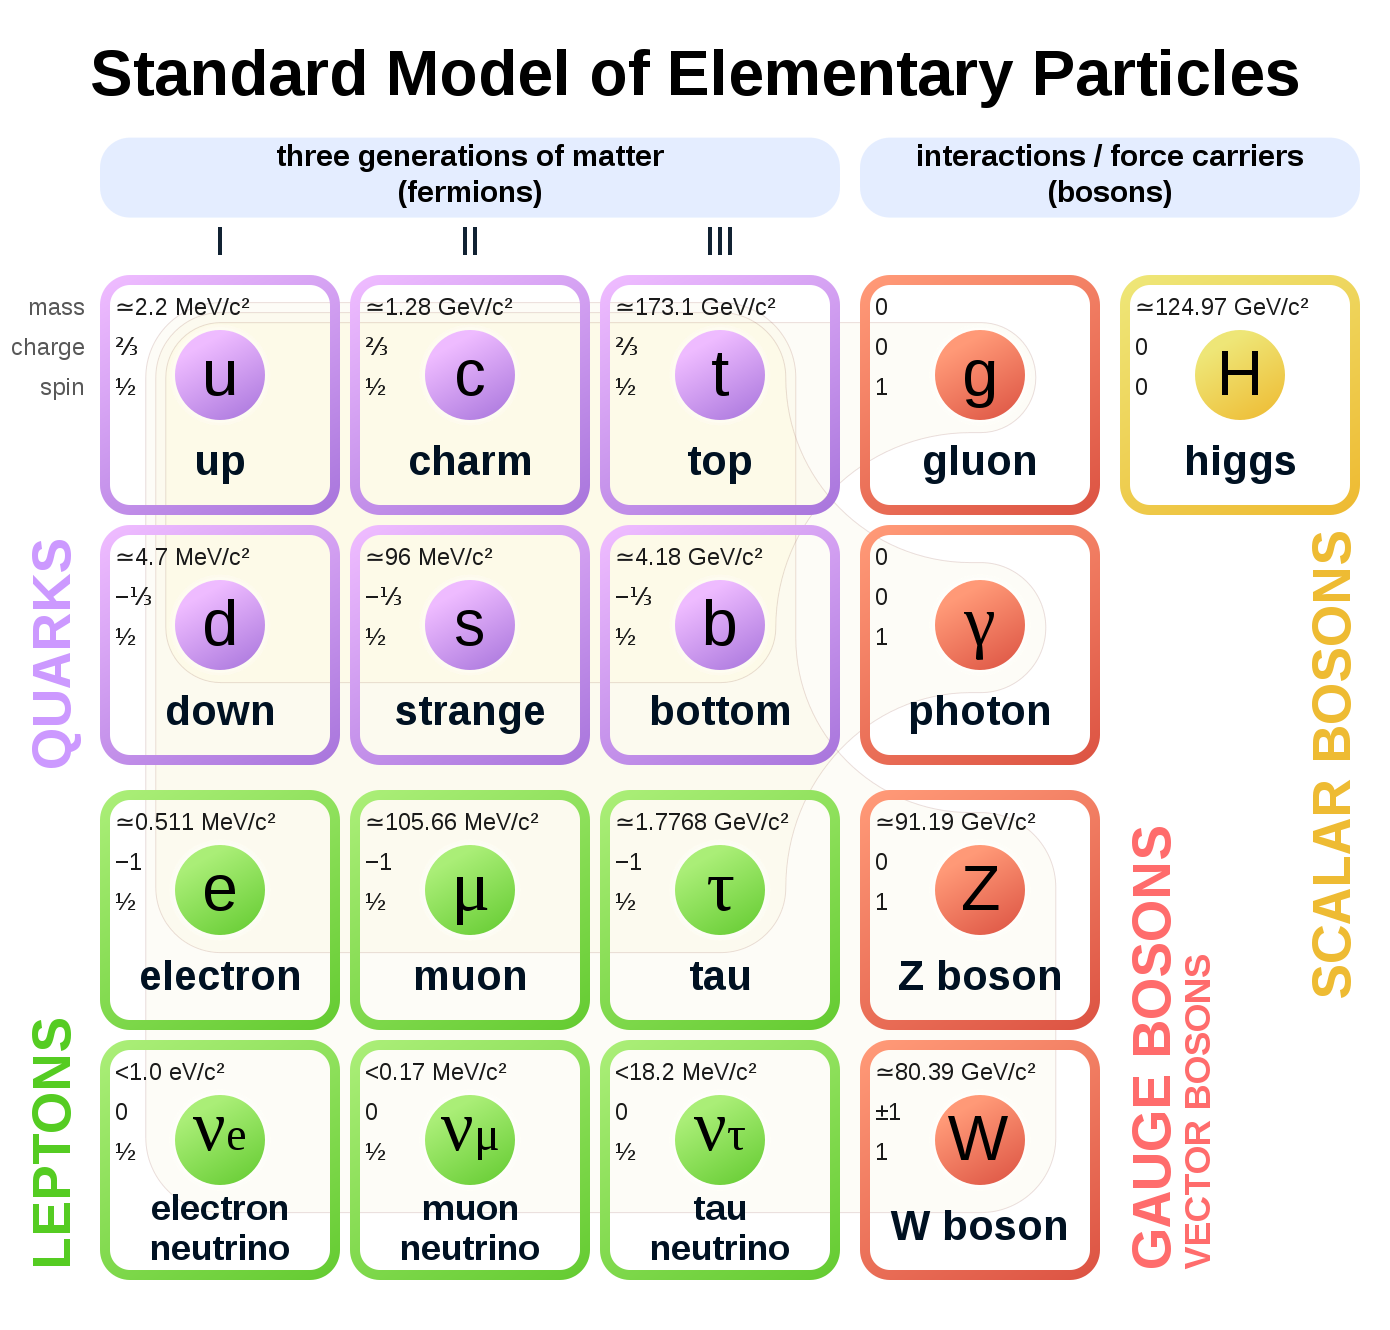
\includegraphics[width=0.6\textwidth ]{figures/theory/sm.png}
  \end{center}\vspace*{-.5cm}
  \caption{Elementary particles of the Standard Model, with their masses charges and spin. Those particles can be divided in two classes: boson (the interaction/force carriers) and the fermions, which are divided in three generations. Source:~\cite{fig_sm_summary}.}
  \label{sm_summary}
  \end{figure}
 

\begin{table}[htp]
  \begin{center}
      \caption{Relative strength (with respect to the strong force) and effective range of action for the four fundamentals interactions.}
    \begin{tabular}{ cccc }
       & Mediator & Relative Strength & Effective Range \\ \hline
      Gravitational & Graviton & $10^{-41}$ & $\infty$ \\ 
      Weak & W and Z bosons & $10^{-16}$ & $10^{-18}$ m \\ 
      Electromagnetic & Photon & $10^{-3}$ & $\infty$ \\ 
      Strong & gluons & $1$ & $10^{-15}$ m\\ \hline
      \end{tabular}
  \label{fundamental_forces}
  \end{center} 
  \end{table}


There are six quark, up and down ($u$ and $d$ - first generation), charm and strange ($c$ and $s$ - second generation), top and bottom ($t$ and $b$ - first generation), in increasing invariant mass order of the generations. Since they interact thought all the three fundamental forces of the SM, they are said to possess electrical charge, flavour and color. Their generational counterparts, the leptons, don't interact via strong interaction, that is why they are said to have only flavours and electric charge. The leptons are electron and electron neutrino ($e$ and $\nu_e$ - first generation), muon and muon neutrino ($\mu$ and $\nu_{\mu}$ - second generation) and tau and tau neutrino ($\tau$ and $\nu_{\tau}$ - third generation). The neutrinos, within the SM, are massless, even though, experimental measurements have shown that they actually have mass~\cite{Patrignani:2016xqp}. Neutrinos are also electrically neutral, meaning that they only interact through weak interactions.

Figure~\ref{sm_summary} also presents the Higgs Boson ($H$) which is part of the SM and shall be discussed later.

Within the Standard Model, the theoretical basis that describe the fundamental interactions are derived from a common principle: the local gauge invariance. According to Salam and Ward~\cite{ward_salam}:


\begin{quote}
  "Our basic postulate is that it should be possible to generate strong, weak and electro-magnetic interaction terms [...], by making local gauge transformations on the kinetic-energy terms in the free Lagrangian for all particles."
\end{quote}

Taking the Quantum Electrodynamics (QED) as an example: the quantum field theory that describes the x


The fundamental theories that compose the Standard Model are all derived from a fundamental principle call 

The electromagnetic force, in the context of fundamental interactions, is describe by a gauge theory called quantum electrodynamics. 




\todo{Electroweak} 

\todo{Higgs}
\todo{discovery}
\todo{Production modes}
\todo{Decay modes}


\todo{Yukawa coupling}

\todo{Higgs results at CMS}

The rare decays of the Higgs boson \cite{20121ATLAS,Chatrchyan:2012xdj} to a quarkonium state and a photon provide a unique sensitivity to the magnitude of the Yukawa couplings of the Higgs boson to quarks \cite{PhysRevD.88.053003, PhysRevD.90.113010,PhysRevLett.114.191803}. These couplings are difficult to access on hadronic collisions through direct decay of Higgs in quark-antiquark, due to the immense background from QCD \cite{PhysRevD.89.033014}. 

Among the channels available to explore Yukawa's couplings of light quarks \cite{PhysRevD.90.113010,PhysRevLett.114.191803} are those with heavy-quarkonia. The rare modes of decay of the \Z boson have attracted attention focused on establishing its sensitivity to New Physics \cite{PEREZ}, being configured as an alternative environment to investigate the Yukawa couplings of the Higgs boson.

% Several estimates of the branching ratio of the Standard Model for the decay of the vector bosons in simple vector meson + photon are available with the latest branching ratio value of the order of $10^{-8}$ and compatible with results published by the ATLAS collaboration~\cite{atlas_results_2016_data}. Thus, the objective of this physics analysis is to explore exclusive rare decays of vector bosons in the CMS experiment using the data taken during 2016.

Also, the exclusive rare decays of vector bosons (\Z, W) provide a favorable environment for testing the factorization of QCD, thus allowing an approach in a context where the power of corrections are definitely under control. The main focus of this kind of analysis are the hadronic radioactive decays, $Z\rightarrow M \gamma$, where M can be a pseudoscalar or a vector meson ($J/ \psi, \phi, \Upsilon_{n}$). 

They offer the perfect way to explore some of the leading order properties of the light-cone distribution amplitudes (LCDAs)~\cite{Grossman2015} of several mesons, but they present a difficulty, considering that in the LHC energy scale the branching ratio of these processes is very small. There are theoretical predictions \cite{PhysRevD.97.016009,PhysRevD.96.116014} that point out a branching ratio for several decay channels in the Standard Model, as shown in the Table \ref{fig:XsecTable}.

\begin{table}[htp]
\begin{center}
%\resizebox{.5\width}{!}{\begin{tabular}{l|llll}
\multicolumn{4}{c}{95\% C.L. Upper Limit} \\
\hline
\hline
& \multicolumn{3}{c}{$\mathcal{B}(Z \rightarrow \Upsilon\gamma)$ $[\times10^{-6}]$}      \\
\cline{2-4}
&  $\Upsilon(1S)$ & $\Upsilon(2S)$ & $\Upsilon(3S)$  \\
\hline
Expected     & $6.4^{+3.1}_{-2.0}$ &  $8.3^{+4.0}_{-2.5}$  & $8.0^{+3.9}_{-2.4}$            \\
Observed     & 9.0 &  12.3  & 11.4      \\
\hline
SM Prediction $[\times10^{-8}]$ & 4.8  &  2.4  & 1.9      \\
\hline
\hline
& \multicolumn{3}{c}{$\mathcal{B}(H \rightarrow \Upsilon\gamma)$ $[\times10^{-4}]$}       \\
\cline{2-4}
&  $\Upsilon(1S)$ & $\Upsilon(2S)$ & $\Upsilon(3S)$ &   \\
\hline
Expected     & $12.5^{+6.1}_{-3.9}$ &  $14.6^{+7.1}_{-4.5}$  & $13.6^{+6.6}_{-4.2}$        \\
Observed     & 11.5 &  13.6  & 12.7     \\
\hline
SM Prediction $[\times10^{-9}]$ & 5.2  &  1.4  & 0.9      \\
\hline
\hline
\end{tabular}

}
%%\begin{table}[htp]
%%\begin{center}
%\begin{tabular}{|c|l|l|}
%\hline
%Description of the Physics Processes  : & Cross Section ( $\sigma$ in pb) & Branching Ratio (BR$_{SM}$): \\ \hline
%H$\rightarrow  \Upsilon(1S) +\gamma$ & 7.1996$\times 10^{-9}$ &5.22$\times 10^{-9}$ \\ \hline
%H$\rightarrow  \Upsilon(2S) +\gamma$ & 1.5242$\times 10^{-9}$ &1.42$\times 10^{-9}$ \\ \hline
%H$\rightarrow  \Upsilon(3S) +\gamma$ & 1.1033$\times 10^{-9}$ &9.10$\times 10^{-10}$ \\ \hline \hline
%%Z$\rightarrow J/ \psi +\gamma$ & 9.9123$\times 10^{-6}$ & 2.99$\times 10^{-6}$ \\ \hline
%Z$\rightarrow  \Upsilon(1S) +\gamma$ & 6.7965$\times 10^{-5}$ &4.88$\times 10^{-8}$ \\ \hline
%Z$\rightarrow  \Upsilon(2S) +\gamma$ & 2.6887$\times 10^{-5}$ &2.44$\times 10^{-8}$ \\ \hline
%Z$\rightarrow  \Upsilon(3S) +\gamma$ & 2.3400$\times 10^{-5}$ &1.88$\times 10^{-8}$ \\ \hline \hline
%H$\rightarrow \gamma\gamma^{*}$ Dalitz Decay & 1.8614$\times 10^{-3}$ & 3.83$\times 10^{-5}$ \\ \hline
%Z$\rightarrow  \mu\mu\gamma_{FSR}$ & 7.9260$\times 10^{-2}$& --- \\ \hline
%
%\end{tabular}
%%\caption{Summary of data samples used for $H/Z \rightarrow \Upsilon(1S,2S,3S)+\gamma$ analysis }
%%\label{Tablebkg}
%%\end{center}
%%\end{table}
%% Ref latex: https://tex.stackexchange.com/questions/112343/beautiful-table-samples
%



%\begin{table}[htp]
%\begin{center}
\begin{tabular}{|c|c|}
\hline
Physics Processes & Branching Ratio (BR$_{SM}$): \\ \hline
H$\rightarrow  \Upsilon(1S) +\gamma$ & 5.22$\times 10^{-9}$ \\ \hline
H$\rightarrow  \Upsilon(2S) +\gamma$ & 1.42$\times 10^{-9}$ \\ \hline
H$\rightarrow  \Upsilon(3S) +\gamma$ & 9.10$\times 10^{-10}$ \\ \hline \hline
Z$\rightarrow  \Upsilon(1S) +\gamma$ & 4.88$\times 10^{-8}$ \\ \hline
Z$\rightarrow  \Upsilon(2S) +\gamma$ & 2.44$\times 10^{-8}$ \\ \hline
Z$\rightarrow  \Upsilon(3S) +\gamma$ & 1.88$\times 10^{-8}$ \\ \hline 
%H$\rightarrow \gamma\gamma^{*}$ Dalitz Decay & 1.8614$\times 10^{-3}$ & 3.83$\times 10^{-5}$ \\ \hline
%Z$\rightarrow  \mu\mu\gamma_{FSR}$ & 7.9260$\times 10^{-2}$& --- \\ \hline

\end{tabular}
%\caption{Summary of data samples used for $H/Z \rightarrow \Upsilon(1S,2S,3S)+\gamma$ analysis }
%\label{Tablebkg}
%\end{center}
%\end{table}
% Ref latex: https://tex.stackexchange.com/questions/112343/beautiful-table-samples


\caption{Summary of cross section and branching ratio for $H/Z \rightarrow \Upsilon(1S,2S,3S)+\gamma  \rightarrow \mu^{+} \mu^{-} +\gamma$ analysis. The effective cross-section will be discussed in section \ref{sec:datasets}.}
%\caption{Summary of cross section and branching ratio for $H/Z \rightarrow \Upsilon(1S,2S,3S)+\gamma  \rightarrow \mu^{+} \mu^{-} +\gamma$ analysis. Assuming that of $\sigma (pp\rightarrow$ H) is 55.614 $pb^{-1}$ and  $\sigma (pp\rightarrow Z \rightarrow \mu\mu$ ) is 57094.5 $pb^{-1}$ with the phase space selection in invariant mass of the dimuon system of $m_{\mu\mu} > 50 GeV$ (Missing References). }
\label{fig:XsecTable}
\end{center}
\end{table}

%Table
 % https://docs.google.com/spreadsheets/d/1zP8P9kp-yFrkMu9bGt4fpIirKAKYlH-w2em_kVkYYKw/edit?usp=sharing
 %Pag2
 
Recent studies on exclusive Higgs boson decays \cite{ISIDORI2014131,PhysRevLett.114.101802,GAO2014366} in final states containing a simple vector meson and a photon have caused interest in these physics topics. It was proposed to use these decays as a possible way to explore non-standard Yukawa couplings of the Higgs boson. Such measures are quite challenging in the LHC environment. The observation of hadronic decays of vector bosons provides could provide a new frontier for the nature of heavy quarkonia production in hadronic collisions.

Along the same lines, the simple exploration of rare SM decays, even in scenarios where anomalous couplings are, in principle, ruled out by direct measurements~\cite{cms_h_to_bb_PhysRevLett.121.121801}, as in the case of this analysis ($H \rightarrow \Upsilon(nS) + \gamma$), are still important as a stress test of the SM and as reference for future measurements. Specially the later one, when you consider that the small predicted cross sections from Table~\ref{fig:XsecTable}, most probably, would imply that an observation of this decay would be unlikely even in the HL-LHC~\cite{hl_lhc}.

This measurement is sensitive to the direct and indirect production (Figure~\ref{direct_indirect}). The \textit{direct} process consists in the decay of boson (Higgs or Z) to a quark anti-quark pair, in which, one of the quarks radiates a photon and the pair hadronizes to a meson (a $\Upsilon(nS)$, for this study), while in \textit{indirect} process, the decay happens to a $\gamma \gamma^{*}(Z)$, with the subsequent decay of the $\gamma^{*}(Z)$ to a quark anti-quark that hadronizes. 


\begin{figure}[!htbp]
  \begin{center}
  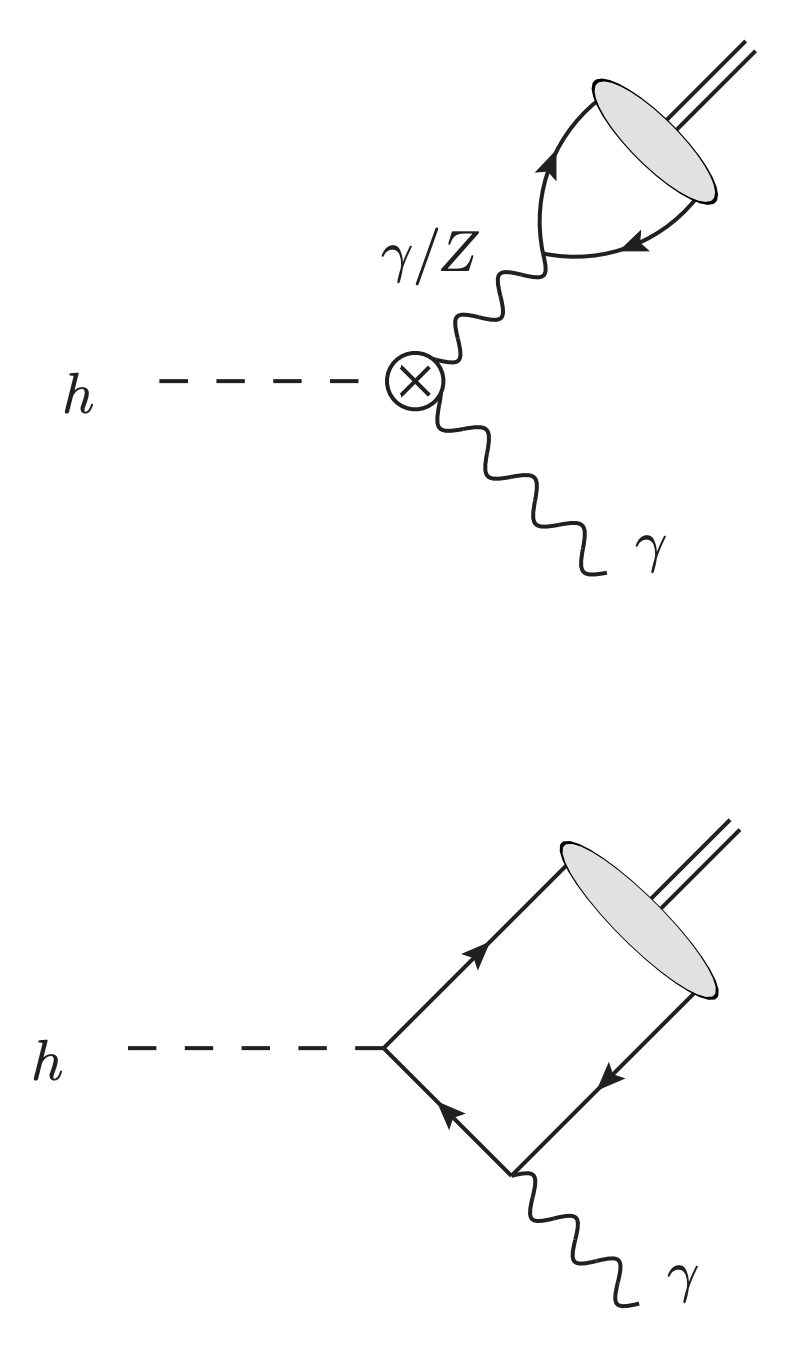
\includegraphics[width=0.35\textwidth ]{figures/theory/direct_indirect.png}
  \end{center}\vspace*{-.5cm}
  \caption{Example of leading order diagrams for the indirect (top) and direct production mechanisms. In the diagrams, the h can also be understood as a Z boson.}
  \label{direct_indirect}
  \end{figure} 

Clearly, only the direct process is sensible to the Yukawa coupling of the boson with the quarks, but, since both processes are indistinguishable in their final state, the in direct process needs to be taken into account. In this study, a dimuon final state is used to tag the $\Upsilon(nS)$.

Even though there is different theoretical predictions for the cross section of this process and its twin brother ($H \rightarrow \text{J/}\Psi + \gamma$), each one taking into account different levels of complexity, the 2013 paper~\cite{PhysRevD.88.053003}, from G. Bodwin, F. Petriello, S. Stoynev and M. Velasco, summarizes very well and in a simpler manner, the most relevant phenomenological results on these decays. For the decay to $J/Psi + \gamma$, the quantum intereference with the indirect amplitude, enhances the directed production, leading to a larger, and potentially observable, cross section. This is not true for the $\Upsilon(nS) + \gamma$ decay, since the interference is destructive, diminishing the cross sections.

Another interesting aspect of this study is that, for both $Hc\bar{c}$ and $Hb\bar{b}$ direct coupling measuremnts are not sensible to the sign of the Yukawa coupling, while the presence of the indirect process in the $H \rightarrow M + \gamma$ ($M$ standing for J/$Psi$ or $\Upsilon(nS)$) decays resolve this ambiguity.

Finally, since the $\Upsilon(nS) + \gamma$ decay has a much smaller cross section, because of the destructive quantum interference between direct and indirect production mechanisms, a small deviation in the $Hb\bar{b}$ Yukawa coupling, can lead a large increase in the expected branching ratio, making this channel sensible any non-Standard Model process that might interfere in this final state. This becomes clear when we look to Figure~\ref{hbb_coup}.

\begin{figure}[!htbp]
  \begin{center}
  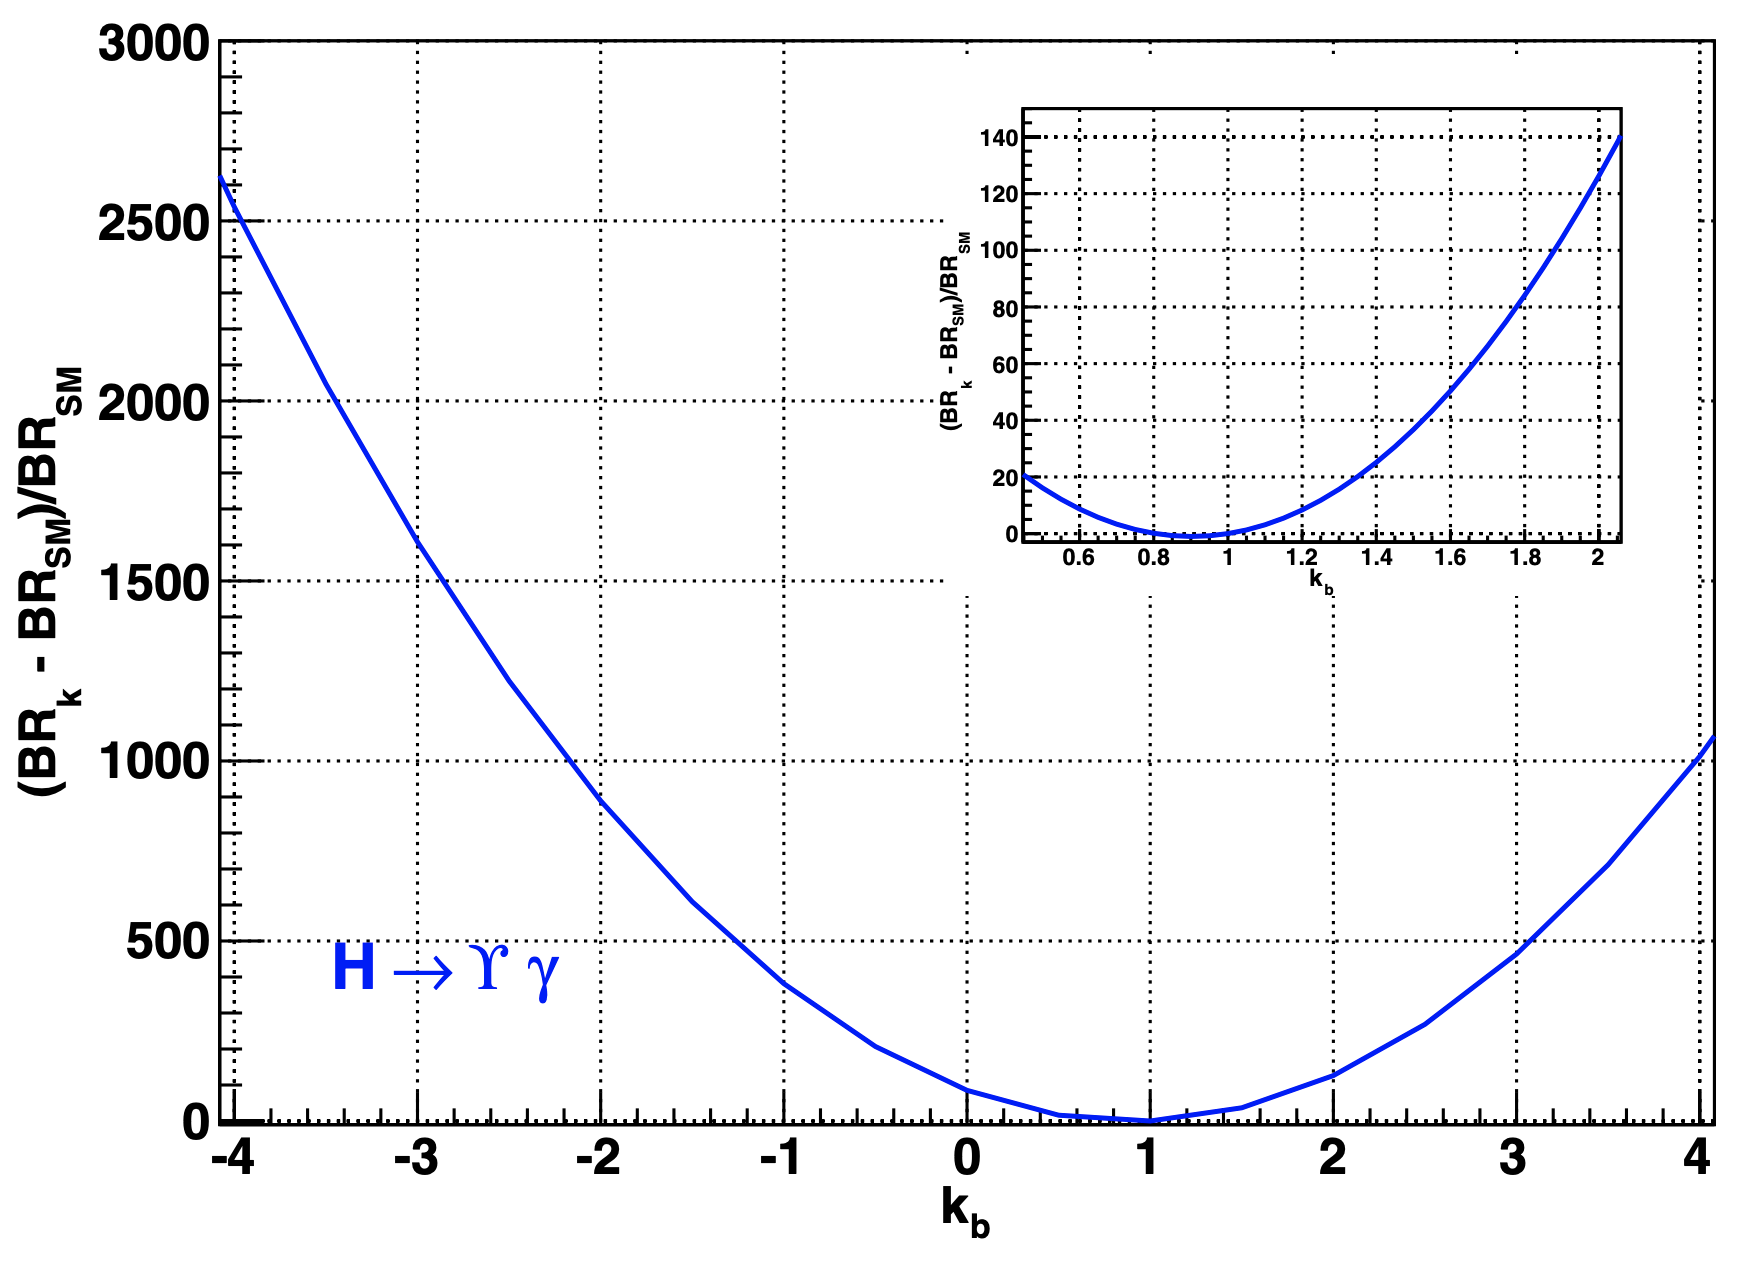
\includegraphics[width=0.6\textwidth ]{figures/theory/hbb_coup.png}
  \end{center}\vspace*{-.5cm}
  \caption{Expected relative variation of the branching ratio for the $H \rightarrow \Upsilon(nS) + \gamma$ to $k_b$, where $k_b = g(Hb\bar{b})/g(Hb\bar{b})_{SM}$ is the ratio for the observed and expected Yukawa coupling oh $Hb\bar{b}$. \cite{PhysRevD.88.053003}}
  \label{hbb_coup}
  \end{figure}


\section{Recent results}

The ATLAS experiment~\cite{atlas_collaboration_2008} already have two results on this decays~\cite{atlas_paper:PhysRevLett.114.121801, atlas_paper_2018:2018txb}. The first one corresponds to data taken from 2015, while the former one, corresponds to data from 2016 (the same data taking period to which this study refers).

The what concerns the most updated result, the study corresponded to 36.1 $fb^{-1}$ at $\sqrt{s} = 13$ TeV and no significant excess was found by the experiment. Upper limits for the were obtained, assuming the Standard Model branching fractions predictions, at 95\% confidence level, according to table~\ref{tab:atlas_results_2018}.

 
\begin{table}[htp]
  \begin{center}

    \begin{tabular}{cc}
      \hline
      Decay & $\mathcal{B}F$ at 95\% \CL \\ \hline
      H$\rightarrow  J/\Psi +\gamma$ & < 4.5$\times 10^{-4}$ \\ 
      H$\rightarrow  \Psi(2S) +\gamma$ & < 2.0$\times 10^{-3}$ \\ 
      H$\rightarrow  \Upsilon(1S) +\gamma$ & < 4.9$\times 10^{-4}$ \\ 
      H$\rightarrow  \Upsilon(2S) +\gamma$ & < 5.9$\times 10^{-4}$ \\ 
      H$\rightarrow  \Upsilon(3S) +\gamma$ & < 5.7$\times 10^{-4}$ \\          
      \hline \hline
      Z$\rightarrow  J/\Psi +\gamma$ & < 2.3$\times 10^{-6}$ \\ 
      Z$\rightarrow  \Psi(2S) +\gamma$ & < 4.5$\times 10^{-6}$ \\ 
      Z$\rightarrow  \Upsilon(1S) +\gamma$ & < 2.8$\times 10^{-6}$ \\ 
      Z$\rightarrow  \Upsilon(2S) +\gamma$ & < 1.7$\times 10^{-6}$ \\ 
      Z$\rightarrow  \Upsilon(3S) +\gamma$ & < 4.8$\times 10^{-6}$ \\        
    \end{tabular}
  \caption{Observed upper limits, by the ATLAS experiment, on the branching fractions for the Higgs and Z decays (last result). Detailed comparisons with the results obtained in this study will be presented in chapter~\ref{chaper_results}.}
  \label{tab:atlas_results_2018}
  \end{center}
  \end{table}

  It is worth it to mention that the ATLAS papers present a broader analysis, including the decays to $J/\Psi +\gamma$ and $\Psi(2S) +\gamma$.


  CMS~\cite{cms_paper} also have a result on $J/\Psi +\gamma$ and $\Psi(2S) +\gamma$ decay channel, of the Higgs and Z boson~\cite{papper_jpsi}. The observed upper limit on the branching fraction for these decays are presented in table~\ref{tab:cms_jpsi_results}.

  \begin{table}[htp]
    \begin{center}

      \begin{tabular}{ ccccc }
        Channel & Polarization  & $\mathcal{B}F$ at 95\% \CL\\
          \hline
          & Unpolarized & $< 1.4\ten{-6}$  \\
          Z$\rightarrow  J/\Psi +\gamma$ & Transverse & $< 1.5\ten{-6}$  \\
          & Longitudinal & $< 1.2\ten{-6}$  \\
          \hline \hline
          H$\rightarrow  J/\Psi +\gamma$ & Transverse & $< 7.6\ten{-4}$  \\
        \end{tabular}
  
  
    \caption{Observed upper limits, by CMS, on the branching fractions for the Higgs and Z decays. The number are compatible with the ones obtained by ATLAS. The results presented for different polarization scenarios of the $J/\Psi$.}
    \label{tab:cms_jpsi_results}
    \end{center}
    \end{table}

No result on the Z and Higgs decays to $\Upsilon(nS) +\gamma$ have been published by CMS, yet.

The results presented here, are a subset of a broader topic related to the rare decays of Standard Model (SM) boson, involving quarkonia. Sticking only to CMS results, we can cite:

\begin{itemize}
  \item Search for Higgs and Z boson decays to $\mathrm{J}/\psi$ or $\Upsilon$ pairs in proton-proton collisions at $\sqrt{s} = $ 13 TeV~\cite{Sirunyan:2676242}.
  \item Observation of the $\mathrm{Z} \to \psi \ell^{+}\ell^{-}$ decay in pp collisions at $\sqrt{s} = $ 13 TeV~\cite{Sirunyan:2623687}. This one specifically, is the first observation a such decay, involving a Z boson.
\end{itemize}

\todo{verificar resultados se outros foram publicados.}

% 
\chapter{Experimental Setup}

The central feature of the CMS apparatus is a superconducting solenoid of 6\unit{m} internal diameter, providing a magnetic field of 3.8\unit{T}. Within the solenoid volume are a silicon pixel and strip tracker, a lead tungstate crystal electromagnetic calorimeter (ECAL), and a brass and scintillator hadron calorimeter (HCAL), each composed of a barrel and two endcap sections. Forward calorimeters extend the pseudorapidity coverage provided by the barrel and endcap detectors. Muons are detected in gas-ionization chambers embedded in the steel flux-return yoke outside the solenoid. 

The silicon tracker measures charged particles within the pseudorapidity range $\abs{\eta} < 2.5$. It consists of 1440 silicon pixel and 15\,148 silicon strip detector modules. For non-isolated particles of $1 < \pt < 10\GeV$ and $\abs{\eta} < 1.4$, the track resolutions are typically 1.5\% in \pt and 25--90 (45--150)\mum in the transverse (longitudinal) impact parameter \cite{TRK-11-001} 

The ECAL consists of 75\,848 lead tungstate crystals, which provide coverage in pseudorapidity $\abs{\eta} < 1.48 $ in a barrel region (EB) and $1.48 < \abs{\eta} < 3.0$ in two endcap regions (EE). Preshower detectors consisting of two planes of silicon sensors interleaved with a total of $3 X_0$ of lead are located in front of each EE detector \cite{Khachatryan:2015hwa}. In the barrel section of the ECAL, an energy resolution of about 1\% is achieved for unconverted or late-converting photons that have energies in the range of tens of GeV. The remaining barrel photons have a resolution of about 1.3\% up to a pseudorapidity of $\abs{\eta} = 1$, rising to about 2.5\% at $\abs{\eta} = 1.4$. In the endcaps, the resolution of unconverted or late-converting photons is about 2.5\%, while the remaining endcap photons have a resolution between 3 and 4\%~\cite{CMS:EGM-14-001}. When combining information from the entire detector, the jet energy resolution amounts typically to 15\% at 10\GeV, 8\% at 100\GeV, and 4\% at 1\TeV, to be compared to about 40\%, 12\%, and 5\% obtained when the ECAL and HCAL calorimeters alone are used. 

Muons are measured in the pseudorapidity range $\abs{\eta} < 2.4$, with detection planes made using three technologies: drift tubes, cathode strip chambers, and resistive plate chambers. The single muon trigger efficiency exceeds 90\% over the full $\eta$ range, and the efficiency to reconstruct and identify muons is greater than 96\%. Matching muons to tracks measured in the silicon tracker results in a relative transverse momentum resolution, for muons with \pt up to 100\GeV, of 1\% in the barrel and 3\% in the endcaps. The \pt resolution in the barrel is better than 7\% for muons with \pt up to 1\TeV~\cite{Sirunyan:2018}. 

A two-tiered trigger system~\cite{Khachatryan:2016bia}. The first level (L1), composed of custom hardware processors, uses information from the calorimeters and muon detectors to select events at a rate of around 100\unit{kHz} within a time interval of less than 4\mus. The second level, known as the high-level trigger (HLT), consists of a farm of processors running a version of the full event reconstruction software optimized for fast processing, and reduces the event rate to around 1\unit{kHz} before data storage.

A more detailed description of the CMS detector, together with a definition of the coordinate system used and the relevant kinematic variables, can be found in Ref.~\cite{Chatrchyan:2008zzk}.  

\todo{falar do sistema de coordenadas e definir $\eta$}

\section{Tracker}
\todo{FAZER!}
\section{Electromagnetic Calorimeter}
\todo{FAZER!}
\section{Hadronic Calorimeter}
\todo{FAZER!}
\section{Muon System}
\todo{FAZER!}
\subsection{DT}
\todo{FAZER!}
\subsection{CSC}
\todo{FAZER!}
\subsection{RPC}
\todo{FAZER!}
\subsection{GEN}
\todo{FAZER!}
\section{Trigger and Data Acquisition}
\todo{FAZER!}
\section{Simulation, reconstruction and computing}
\todo{FAZER!}
\section{Particle Flow Algorithim}
\todo{FAZER!}

% \chapter{Physics Analysis}

\todo{DEFINIR A ANALISE}

\todo{EXPLICAR O PROCESSO E EXEMPLOS DE GRAFICO}

\todo{EXPLICAR A ESTRATEGIA}

\section{Datasets and simulated events} \label{datasets_and_MC_samples}

\subsection{Data samples}

The data sample used in this analysis consists of the 2016 13 \TeV run
with 25 ns bunch separation recorded by CMS. This data sample is composed only by events that were certified from all CMS subsystems and and reconstruction specialist as good for physics analysis.

This data sample corresponds to 35.86 $fb^{-1}$ of integrated luminosity~\cite{CMS-PAS-LUM-17-001}.


% \begin{table}[htp]
% \begin{center}
% %\resizebox{.5\width}{!}{\begin{tabular}{l|llll}
\multicolumn{4}{c}{95\% C.L. Upper Limit} \\
\hline
\hline
& \multicolumn{3}{c}{$\mathcal{B}(Z \rightarrow \Upsilon\gamma)$ $[\times10^{-6}]$}      \\
\cline{2-4}
&  $\Upsilon(1S)$ & $\Upsilon(2S)$ & $\Upsilon(3S)$  \\
\hline
Expected     & $6.4^{+3.1}_{-2.0}$ &  $8.3^{+4.0}_{-2.5}$  & $8.0^{+3.9}_{-2.4}$            \\
Observed     & 9.0 &  12.3  & 11.4      \\
\hline
SM Prediction $[\times10^{-8}]$ & 4.8  &  2.4  & 1.9      \\
\hline
\hline
& \multicolumn{3}{c}{$\mathcal{B}(H \rightarrow \Upsilon\gamma)$ $[\times10^{-4}]$}       \\
\cline{2-4}
&  $\Upsilon(1S)$ & $\Upsilon(2S)$ & $\Upsilon(3S)$ &   \\
\hline
Expected     & $12.5^{+6.1}_{-3.9}$ &  $14.6^{+7.1}_{-4.5}$  & $13.6^{+6.6}_{-4.2}$        \\
Observed     & 11.5 &  13.6  & 12.7     \\
\hline
SM Prediction $[\times10^{-9}]$ & 5.2  &  1.4  & 0.9      \\
\hline
\hline
\end{tabular}

}
% %\begin{table}[htp]
%\begin{center}
\begin{tabular}{|l|c|}
\hline
Description of the data samples : & Luminosity - $\mathcal{L}$  (in  fb$^{-1}$): \\ \hline
\small{/MuonEG/Run2016B-03Feb2017\_ver2-v2/MINIAOD} & 5.784 \\ \hline
\small{/MuonEG/Run2016C-03Feb2017-v1/MINIAOD} & 2.573 \\ \hline
\small{/MuonEG/Run2016D-03Feb2017-v1/MINIAOD} & 4.248 \\ \hline
\small{/MuonEG/Run2016E-03Feb2017-v1/MINIAOD} & 4.009 \\ \hline
\small{/MuonEG/Run2016F-03Feb2017-v1/MINIAOD} & 2.704 \\ \hline
\small{/MuonEG/Run2016F-03Feb2017-v1/MINIAOD} & 0.397 \\ \hline
\small{/MuonEG/Run2016G-03Feb2017-v1/MINIAOD} & 7.540 \\ \hline
\small{/MuonEG/Run2016H-03Feb2017\_ver2-v1/MINIAOD} & 8.391 \\ \hline
\small{/MuonEG/Run2016H-03Feb2017\_ver3-v1/MINIAOD} & 0.215 \\ \hline
\textbf{Total} & \textbf{35.86}  \\ \hline

\end{tabular}
%\caption{Summary of data samples used for $H/Z \rightarrow \Upsilon(1S,2S,3S)+\gamma$ analysis }
%\label{Tablebkg}
%\end{center}
%\end{table}


% \caption{Primary datasets from 2016 using the full dataset consists of 35.86 $fb^{-1}$ of integrated luminosity~\cite{CMS-PAS-LUM-17-001}.}
% \label{tab:golden}
% \end{center}
% \end{table}



\subsection{Simulated datasets}
\label{sec:datasets}

\todo{PILE-UP reweighting}

A summary of the signal and background Monte Carlo (from here on, simply called MC) samples used is presented in Table~\ref{tab:MC}. These simulated data are comparable with the proton-proton collision using 2016 data conditions and the pile-up events are added to the simulated event in this step. The pile-up events distribution used is around 23 events, as recomended by CMS. Detector response in the MC samples is simulated using a detailed description of the CMS detector, based on \GEANTfour~\cite{Agostinelli:2002hh}.

The signal MC samples are simulated for the Higgs bosons decaying to $\Upsilon(nS) (\rightarrow \mu\mu) + \gamma$  channels with POWHEG v2.0~\cite{powheg2_1,powheg2_2,powheg2_3}, at next-to-leading order (NLO) of Feynman graphs computation, for the following production modes: gluon-gluon fusion (ggF), vector boson fusion (VBF), associated production (VH) and associated top production (ttH), with cross-section sumarized at table \ref{tab:MC}. A extensive review of these production modes can be found at~\cite{DJOUADI20081}. The \PYTHIA 8 generator~\cite{SJOSTRAND2008852,Sjostrand:2014zea} is used for hadronization and fragmentation with underlying event tune CUETP8M1~\cite{Khachatryan:2015pea}. The parton distribution functions (pdf) NNPDF3.0~\cite{NNPDF3} are used. 

 For Z decaying to $\Upsilon(nS) (\rightarrow \mu\mu) + \gamma$  channels, the signal samples are simulated with \MADGRAPH5 $\_$\MCATNLO 2.6.0 matrix element generator~\cite{Alwall2014} at next leading order and the \PYTHIA 8 generator~\cite{SJOSTRAND2008852,Sjostrand:2014zea} for hadronization and fragmentation with underlying event tune CUETP8M1~\cite{Khachatryan:2015pea}.

The Drell-Yan process, $pp \rightarrow \Z \rightarrow \mu\mu \gamma$, results in the same final state as the signal. This process exhibits a peak in the three-body invariant mass, $m_{\mu\mu\gamma}$, at the \Z boson mass, $m_{Z}$, and it is a ressonant background for this channel, therefore referred to as a Peaking Background. 

It is taken into account when deriving the upper limit on the branching fraction for Z$\rightarrow \Upsilon(nS) + \gamma \rightarrow \mu\mu + \gamma$. The \MADGRAPH5 $\_$\MCATNLO 2.6.0 matrix element generator~\cite{Alwall2014} at leading order, interfaced with \PYTHIA 8.226 for parton showering and hadronization with tune CUETP8M1~\cite{Khachatryan:2015pea}, is used to generate a sample of these resonant background events. The photons in these events are all produced as final-state radiation from the $ Z \rightarrow \mu\mu$ decay and therefore the $m_{\mu\mu\gamma}$ distribution peaks at the \Z boson mass and there is no continuum contribution.  

Similarly, the Higgs boson Dalitz decay~\cite{PhysRevD.55.5647}, $H \rightarrow \gamma^{*} \gamma\rightarrow \mu\mu + \gamma$, is a Peaking Background (resonant) to $H \rightarrow \Upsilon(nS) \rightarrow \mu\mu + \gamma$. It is simulated at NLO with \MADGRAPH5 $\_$\MCATNLO 2.6.0 matrix element generator~\cite{Alwall2014} at next-to-leading order and the \PYTHIA 8 generator~\cite{SJOSTRAND2008852,Sjostrand:2014zea} for hadronization and fragmentation with underlying event tune CUETP8M1~\cite{Khachatryan:2015pea}. This Higgs Dalitz Decay sample, was generated only for the ggF production mode, but its cross-section was rescaled to the full Higgs cross-section. This process will present a small contribuition of selected events, so this approximation should be sufficient for the Higgs Peaking Background modeling.

There are also background processes that do not give resonance peaks in the three-body invariant mass spectrum. They are modeled from data, as it will be explained latter in more details.
 
\begin{table}[htp]
\begin{center}
%
%\begin{tabular}{lcccc} \hline
%Physics Processes &  $\sigma$ in pb   & Branching Ratio (BR$_{SM}$) & Generator & Sample Type \\ \hline
%H$\rightarrow  \Upsilon(1S) +\gamma$ & 7.1996$\times 10^{-9}$ &5.22$\times 10^{-9}$ & PYTHIA8 & Signal \\ 
%H$\rightarrow  \Upsilon(2S) +\gamma$ & 1.5242$\times 10^{-9}$ &1.42$\times 10^{-9}$  & PYTHIA8 & Signal \\ 
%H$\rightarrow  \Upsilon(3S) +\gamma$ & 1.1033$\times 10^{-9}$ &9.10$\times 10^{-10}$ & PYTHIA8 & Signal \\ \hline
%Z$\rightarrow  \Upsilon(1S) +\gamma$ & 6.7965$\times 10^{-5}$ &4.88$\times 10^{-8}$ & PYTHIA8 & Signal \\ 
%Z$\rightarrow  \Upsilon(2S) +\gamma$ & 2.6887$\times 10^{-5}$ &2.44$\times 10^{-8}$ &  PYTHIA8 & Signal \\
%Z$\rightarrow  \Upsilon(3S) +\gamma$ & 2.3400$\times 10^{-5}$ &1.88$\times 10^{-8}$ &  PYTHIA8 & Signal \\  \hline \hline
%H$\rightarrow \gamma\gamma^{*}$ Dalitz Decay & 1.8614$\times 10^{-3}$ & 3.83$\times 10^{-5}$ & --- & Peaking Background \\ 
%Z$\rightarrow  \mu\mu\gamma_{FSR}$ & 7.9260$\times 10^{-2}$& --- & --- & Peaking Background \\ \hline
%\end{tabular}





\begin{tabular}{lcccc} \hline
Physics Processes & Branching Ratio (BR$_{SM}$)  & Effective $\sigma$ (in pb) & Generator & Sample Type \\ \hline
H$\rightarrow  \Upsilon(1S) +\gamma$ &5.22$\times 10^{-9}$ & 7.14$\times 10^{-9}$ & \POWHEG 2.0 & Signal \\ 
H$\rightarrow  \Upsilon(2S) +\gamma$ &1.42$\times 10^{-9}$ &  1.51$\times 10^{-9}$ & \POWHEG 2.0 & Signal \\ 
H$\rightarrow  \Upsilon(3S) +\gamma$ &9.10$\times 10^{-10}$ & 1.10$\times 10^{-9}$ & \POWHEG 2.0 & Signal \\ \hline
Z$\rightarrow  \Upsilon(1S) +\gamma$ &4.88$\times 10^{-8}$ & 6.80$\times 10^{-5}$ & \MADGRAPH5  & Signal \\ 
Z$\rightarrow  \Upsilon(2S) +\gamma$ &2.44$\times 10^{-8}$ & 2.69$\times 10^{-5}$ &  \MADGRAPH5  & Signal \\
Z$\rightarrow  \Upsilon(3S) +\gamma$ &1.88$\times 10^{-8}$ & 2.34$\times 10^{-5}$ &  \MADGRAPH5  & Signal \\  \hline \hline
H Dalitz Decay & 3.83$\times 10^{-5}$ & 2.13$\times 10^{-3}$ &\MADGRAPH5 & Resonant Background \\ 
Z$\rightarrow  \mu\mu\gamma_{FSR}$ & --- & 7.93 $\times 10^{-2}$ & \MADGRAPH5  & Resonant Background \\ \hline
\end{tabular}
\caption{Datasets simulated (MC) for 2016 conditions. Assuming that $\sigma (pp\rightarrow$ H), taking into consideration all the simulated Higgs production modes, is 55.13 $pb$~\cite{CERNYellowReportPageAt13TeV} and  $\sigma (pp\rightarrow Z \rightarrow \mu\mu$ ) is 57094.5 $pb$, including the next-to-next-to-leading order
(NNLO) QCD contributions, and the next-to-leading order (NLO) electroweak corrections from fewz 3.1~\cite{FEWZ} calculated using the NLO PDF set NNPDF3.0, with the phase space selection in invariant mass of the dimuon system of $m_{\mu\mu} > 50$ GeV. For the Higgs Dalitz $\sigma$, we consider only the gluon fusion contribution ($\sigma_{\text{ggF}}  = $ 48.6 $pb$)~\cite{CERNYellowReportPageAt13TeV}. The Higgs Dalitz Decay $BR_{SM}$ and the $Z \rightarrow \mu\mu\gamma_{FSR}$ were obtained with MCFM 6.6~\cite{CAMPBELL201010} (as in the CMS search for Higgs Dalitz Decay in at $\sqrt{s} =$ 8 TeV~\cite{dalitz_decay_8_Tev}) and with \MADGRAPH5 $\_$\MCATNLO, respectively. The $BR^{PDG}_{\Upsilon(1S,2S,3S) \rightarrow \mu\mu} = \text{(2.48, 1.93, 2.18)} \times 10^{-2}$ is quoted from Particle Data Group report (PDG)~\cite{Patrignani:2016xqp}. The "Effective $\sigma$" for the signal samples is $\sigma(pp \rightarrow Z(H)) \times BR_{SM} \times BR^{PDG}_{\Upsilon(nS) \rightarrow \mu\mu}$.}
\label{tab:MC}
\end{center}
\end{table}

The number of simulated events is is rescaled by the Effective $\sigma$, from table~\ref{tab:MC}, in order to match 35.86 $fb^{-1}$ of integrated luminosity, from the recorded data. Being $N = \sigma \mathcal{L}$, $N$ in the number of events for a process, $\sigma$ is the cross-section and $\mathcal{L}$ is the integrated luminosity, the reweighting factor, for a simulated sample is:

\begin{equation}
\label{eqn:mc_weight}
w_{MC} = \frac{\sigma \mathcal{L}}{N_{sim}},
\end{equation}
where $N_{sim}$ is the number of simulated events for a specific process.

The simulated sample are also corrected by the data pile-up distribution, since the pileup distribution of MC is different from the pileup distribution of data. The way to correct the MC is to assign a weight to each bin of the MC pileup distribution, with repect to the data. The rescaling is defined as the ration between normalized Pile-up (PU) distribution for Data and MC.

\begin{equation}
\label{eqn:mc_weight}
w_{PU}(n) = \frac{P^{Data}_{PU}(n)}{P^{Sim}_{PU}(n)},
\end{equation}
where $n$ is the number of interaction per bunch crossing (pile-up).

\section{Contribution of the \texorpdfstring{$\Upsilon(nS)$} p polarisation}
\label{sec:polarization}

% Tem que ter esse erro de digitacao no titulo senao nao compila.
Measurements of quarkonium polarization observables may yield information about quarkonium production mechanisms that are not available from the study of unpolarized cross sections alone. The three polarization states of a $J = 1$ quarkonium can be specified in terms of a particular coordinate system in the rest frame of the quarkonium. This coordinate system is often called the "spin-quantization frame". 

In a hadron collider, $\Upsilon(1S,2S,3S)$ are reconstructed through their electromagnetic decays into a lepton pair. The information about the polarization of the quarkonium state is encoded in the angular distribution of the leptons. This angular distribution is usually described in the quarkonium rest frame with respect to a particular spin-quantization frame~\cite{Brambilla:2011bph}. The polarization of the  $\Upsilon(1S,2S,3S)$ is not simulated for signal MC sample and we only apply a reweighting scale factor to each event and so we can emulate the polarization effects~\cite{PhysRevD.83.031503}. Figure \ref{fig:ZUpsilonPolarization} present the distributions of $\cos \Theta$ of $\Upsilon \rightarrow \mu\mu$, 
% and $\gamma^{*} \rightarrow \mu\mu$, 
where $\Theta$ is the angle between the positive muon and the $\Upsilon$ in the Z (Higgs) rest-frame. At Table \ref{fig:polTable} we show the the analytical functions used to describe the extremes scenarios (Unpolarized, Transverse Polarization and Longitudinal Polarization) reweighting, presented in this analysis. 

It is worth stating that, for the Higgs decay, on the Transverse Polarization is considered. For the Z decay, because of its spin nature, the Unpolarized scenario is used as the nominal one, and the effects of the two other extremes (Transverse Polarization and Longitudinal Polarization) are quoted as systematics.


% \begin{figure}[!htbp]
% \begin{center}
% 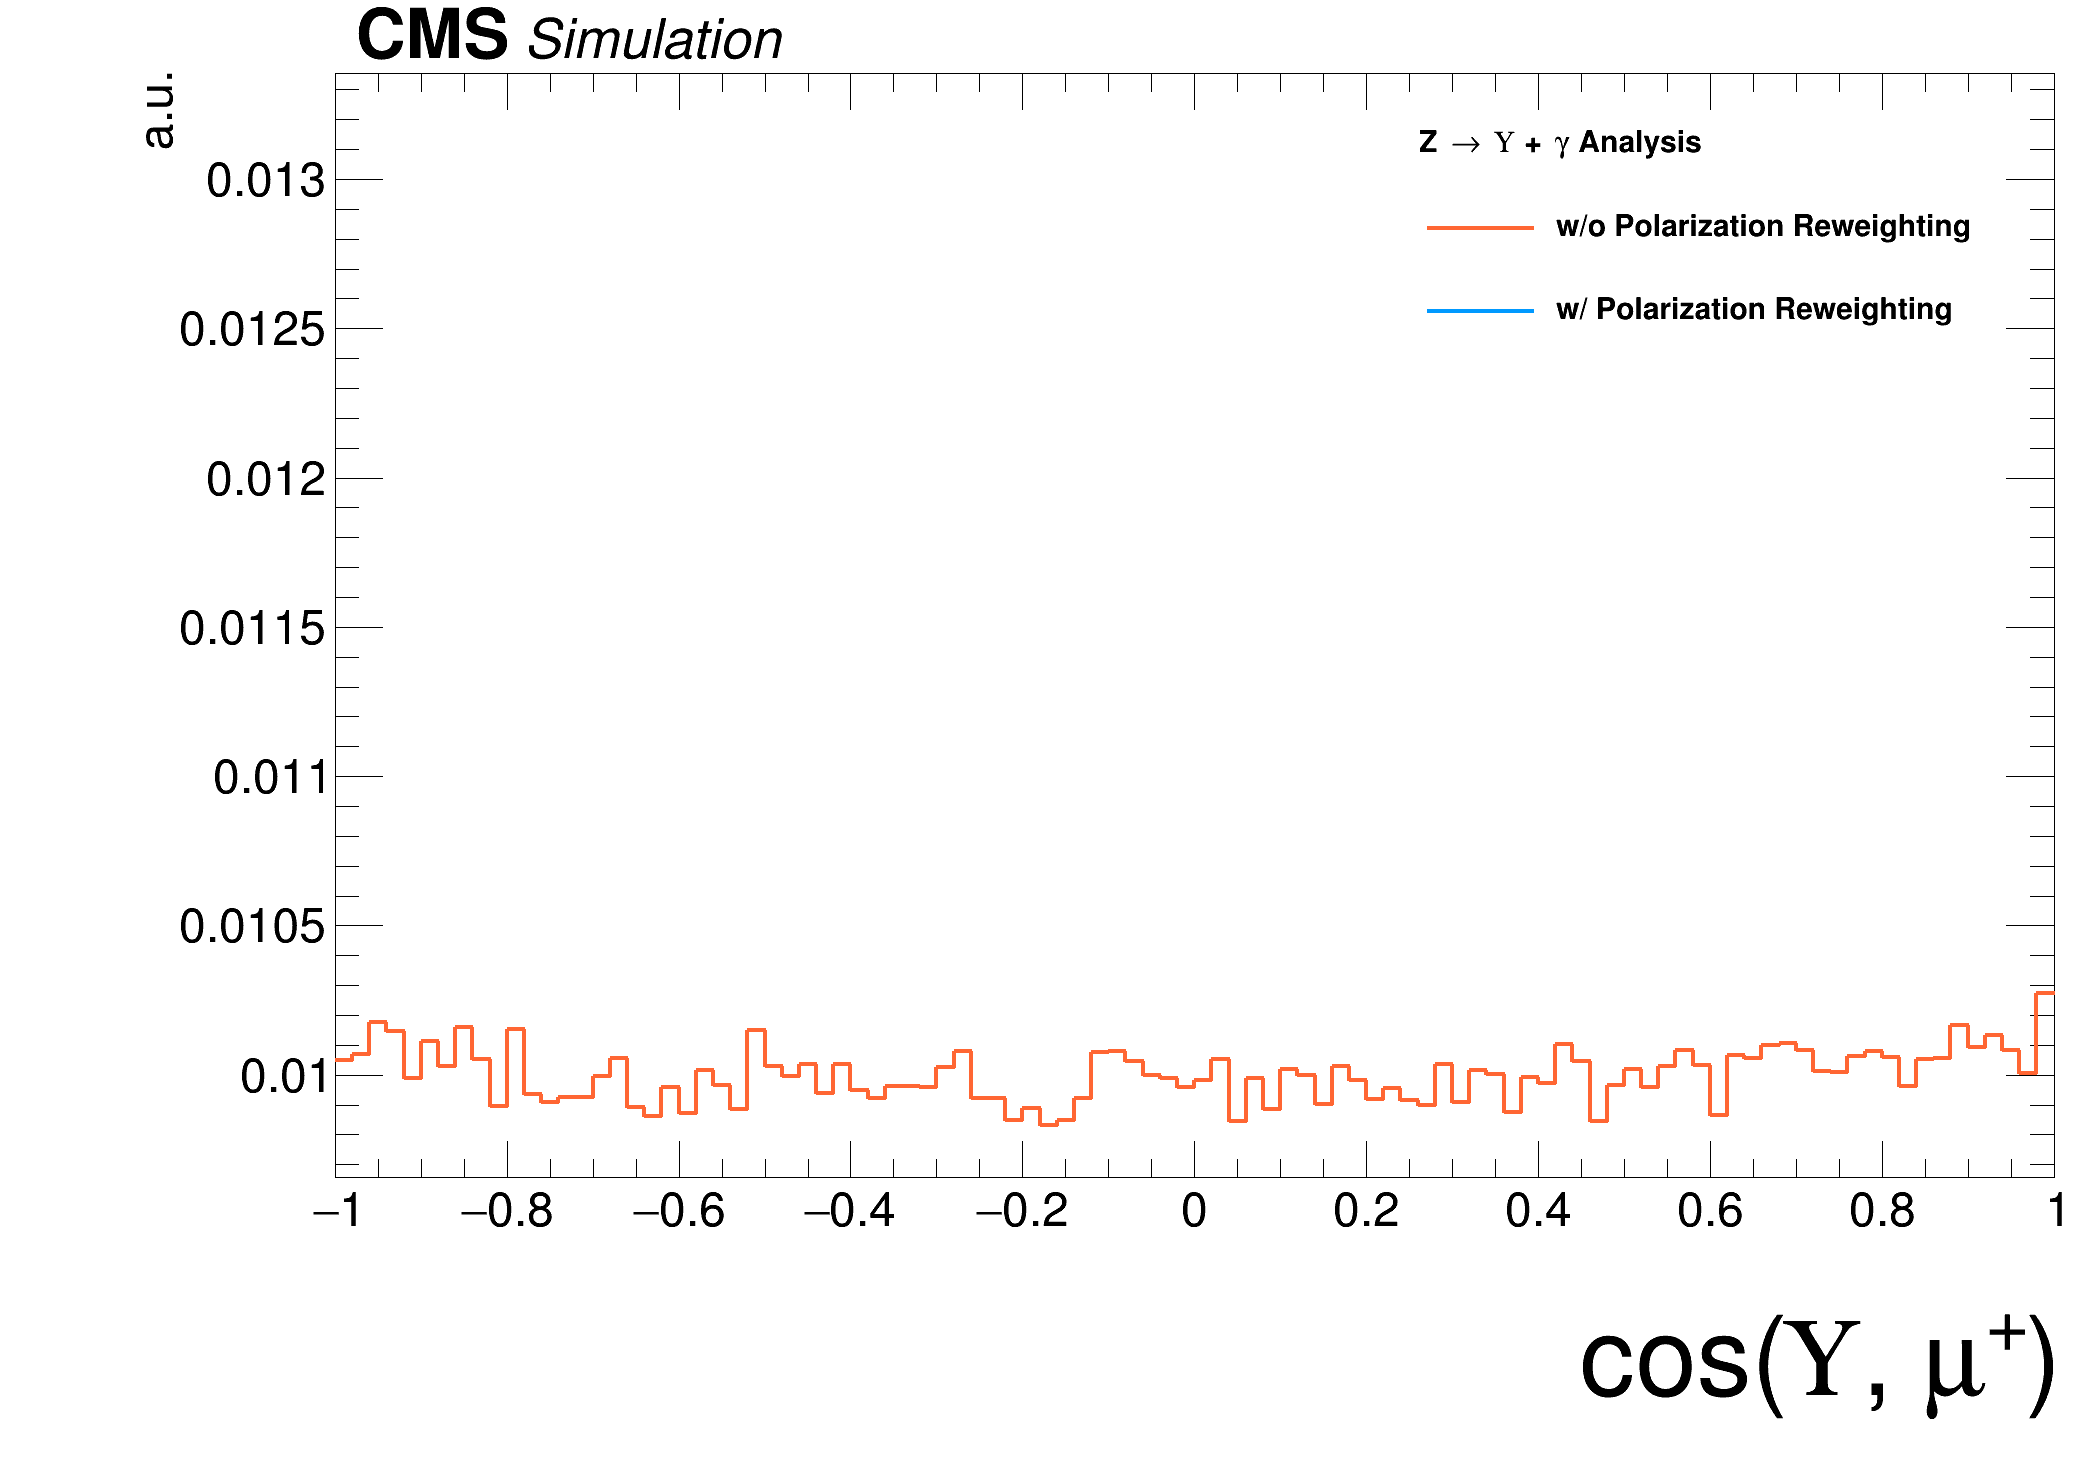
\includegraphics[width=0.50\textwidth]{figures/outputPlots/HtoUpsilon_Cat0_ZZZZZ/mc/polarizatioReweight/h_Gen_COS_theta}
% \end{center}\vspace*{-.5cm}
% \caption{Distributions of $\cos \theta$ of $\Upsilon \rightarrow \mu\mu$ and $\gamma^{*} \rightarrow \mu\mu$ The orange distribution is the $H \rightarrow  \Upsilon(1S,2S,3S) + \gamma$ sample before reweighting; the blue distribution is $H \rightarrow  \Upsilon(1S,2S,3S)$ sample after reweighting.}
% \label{fig:HUpsilonPolarization}
% \end{figure}


\begin{figure}[!htbp]
\begin{center}
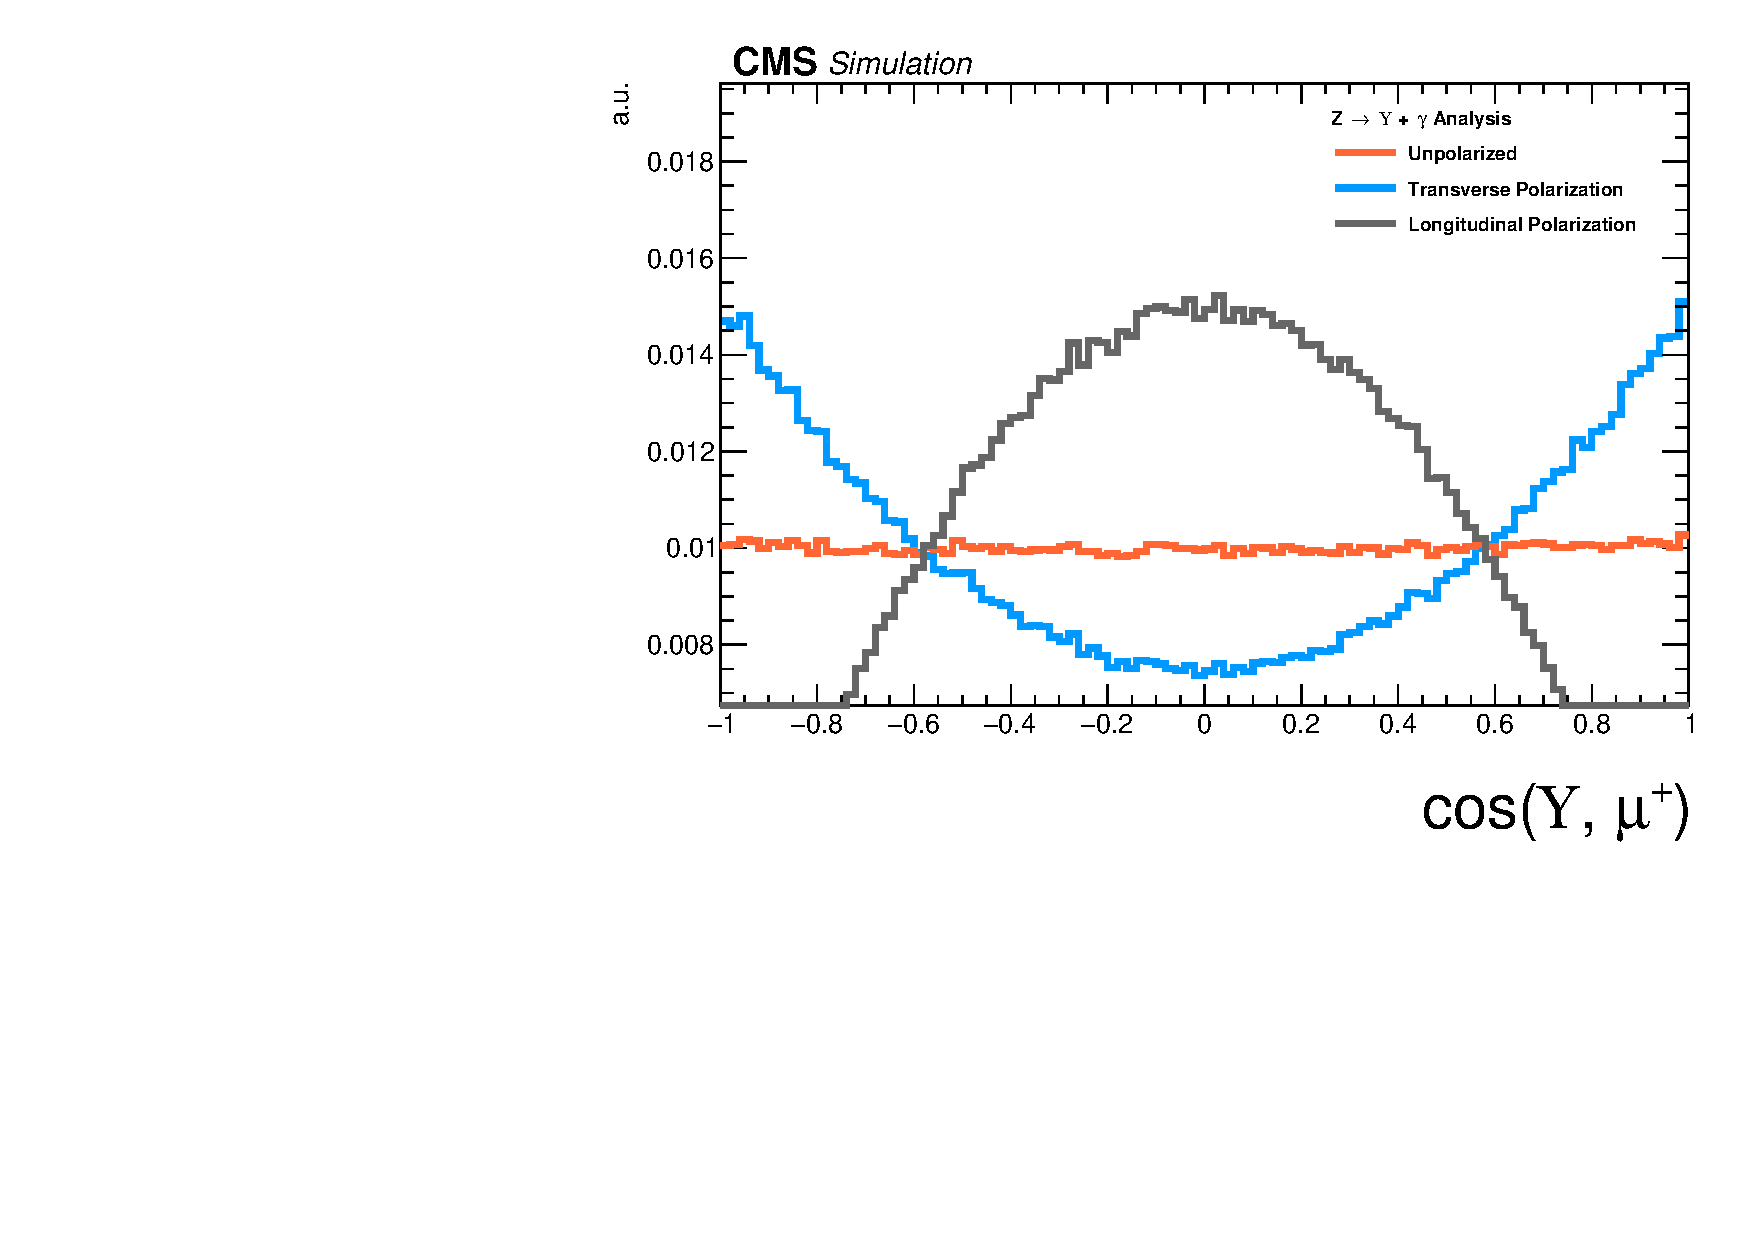
\includegraphics[width=0.80\textwidth]{figures/outputPlots/ZtoUpsilon_Cat0_ZZZZZ/mc/polarizatioReweight/h_Gen_COS_theta_extremes}
\end{center}\vspace*{-.5cm}
\caption{Distributions of $\cos \theta$ of $\Upsilon \rightarrow \mu\mu$ and $\gamma^{*} \rightarrow \mu\mu$ The orange distribution is the $Z \rightarrow  \Upsilon(1S,2S,3S) + \gamma$ sample before reweighting (Unpolarized); the blue and gray distributions are $Z \rightarrow  \Upsilon(1S,2S,3S)$ sample after reweighting, for the Transverse and Longitudinal Polarization.}
\label{fig:ZUpsilonPolarization}
\end{figure}


\begin{table}[htp]
\begin{center}
%\begin{table}[htp]
%\begin{center}
%\begin{tabular}{|cl }
\begin{tabular}{|l l l |}

\hline

$J_{Z}$ & Polarisation Scenario & Analytic Description \\ \hline
$\pm$ 1  & Transverse &  3/4 $\times (1 + (\cos \theta)^{2})$ \\ \hline
0  & Longitudinal & 3/2 $\times (1- (\cos \theta)^{2})$ \\ \hline

\end{tabular}
%\caption{Summary of data samples used for $H/Z \rightarrow \Upsilon(1S,2S,3S)+\gamma$ analysis }
%\label{Tablebkg}
%\end{center}
%\end{table}
% Ref latex: https://tex.stackexchange.com/questions/112343/beautiful-table-samples


\caption{Summary of the impact of reweighted of polarization contribution using several scenarios.}
\label{fig:polTable}
\end{center}
\end{table} 



\section{Kinematical studies using MC generator}


Using the \PYTHIA 8.226 generator, the Monte Carlo signals are produced for Higgs (Z) boson events decaying in ($\Upsilon$(1S,2S,3S)) + $\gamma$, which are highly boosted. Observing the kinematic generator level distributions in Figure \ref{fig:MC_ZtoUpsilon_Cat0} for Z boson and Figure \ref{fig:MC_HtoUpsilon_Cat0} for Higgs boson, we could conclude that the high-\ET (transverse energy, with respect to the beam line) photon will be back-to-back to the $\Upsilon$ particles being possible to apply an isolation selection to identify a photon in this kinematic topology. Also, we can observe those transverse momenta of the leading/trailing \PT (transverse momemtum, with respect to the beam line) muon~\footnote{In this study we define leading muon and the muon, decaying from the $\Upsilon$, with highest \PT. Trailing muon is the one with the second hight \PT.} and the photon and distances $\Delta R=\sqrt{\Delta\eta^2 + \Delta\phi^2}$ between the two muons and between the muons and the photon are a good variable that can be used to discriminate the contribution between signal and background events. The leading muon transverse momentum can be greater than 45(30)\GeV and trailing muon is greater than 10(20)\GeV in Higgs(Z) decay.
$\Delta R$ distributions of the two muons and between the muons and the photon in the both cases show that the two muons are very close and the photon is back-to-back in relation of dimuon system. Another feature of this kinematic topology is that the production vertex between muons produced in $\Upsilon$ decaying events and the high-\ET photon is very well defined.  

% Concerning the main reducible background (combinatorial background), it is due to Drell-Yan process where the photon comes from the initial-state radiation (ISR) or final-state radiation (FSR) and background reducible events are produced from Drell-Yan with jet associate and inclusive quarkonium production, where the jet in both processes is misidentified as a photon in reconstruction level. For the analysis, besides the peaking background, most of the background contributions will be modeled from data. 

\begin{figure}[!htbp]
\begin{center}
% Muon
%\hspace*{1.cm}
\includegraphics[width=0.45\textwidth]{figures/outputPlots/ZtoUpsilon_Cat0_ZZZZZ/mc/unpolarized/h_Gen_Mu_pt}
%\hspace*{1.cm}
\includegraphics[width=0.45\textwidth]{figures/outputPlots/ZtoUpsilon_Cat0_ZZZZZ/mc/unpolarized/h_Gen_Mu_eta}
%\hspace*{1.cm}
\includegraphics[width=0.45\textwidth]{figures/outputPlots/ZtoUpsilon_Cat0_ZZZZZ/mc/unpolarized/h_Gen_Mu_phi}
%\hspace*{1.cm}
%Delta R mu_trading and mu_leading
\includegraphics[width=0.45\textwidth]{figures/outputPlots/ZtoUpsilon_Cat0_ZZZZZ/mc/unpolarized/h_Gen_deltaR_Leading_Trailing}
%\hspace*{1.cm}
%Photon
\includegraphics[width=0.45\textwidth]{figures/outputPlots/ZtoUpsilon_Cat0_ZZZZZ/mc/unpolarized/h_Gen_Photon_pt}
%\hspace*{1.cm}
\includegraphics[width=0.45\textwidth]{figures/outputPlots/ZtoUpsilon_Cat0_ZZZZZ/mc/unpolarized/h_Gen_Photon_eta}
%\hspace*{1.cm}
\includegraphics[width=0.45\textwidth]{figures/outputPlots/ZtoUpsilon_Cat0_ZZZZZ/mc/unpolarized/h_Gen_Photon_phi}
%\hspace*{1.cm}
%Delta R mu+ photon
\includegraphics[width=0.45\textwidth]{figures/outputPlots/ZtoUpsilon_Cat0_ZZZZZ/mc/unpolarized/h_Gen_deltaR_Mu_Photon}
%\hspace*{1.cm}
%Upsilon
%\includegraphics[width=0.25\textwidth]{figures/outputPlots/ZtoUpsilon_Cat0_ZZZZZ/mc/unpolarized/h_Gen_Upsilon_Pt}
%\hspace*{1.cm}
%\includegraphics[width=0.25\textwidth]{figures/outputPlots/ZtoUpsilon_Cat0_ZZZZZ/mc/unpolarized/h_Gen_Upsilon_eta}
%\hspace*{1.cm}
%\includegraphics[width=0.25\textwidth]{figures/outputPlots/ZtoUpsilon_Cat0_ZZZZZ/mc/unpolarized/h_Gen_Upsilon_phi}
%\hspace*{1.cm}
%Z
%\includegraphics[width=0.25\textwidth]{figures/outputPlots/ZtoUpsilon_Cat0_ZZZZZ/mc/unpolarized/h_Gen_Z_Pt}
%\hspace*{1.cm}
%\includegraphics[width=0.25\textwidth]{figures/outputPlots/ZtoUpsilon_Cat0_ZZZZZ/mc/unpolarized/h_Gen_Z_eta}
%\hspace*{1.cm}
%\includegraphics[width=0.25\textwidth]{figures/outputPlots/ZtoUpsilon_Cat0_ZZZZZ/mc/unpolarized/h_Gen_Z_phi}
%\hspace*{1.cm}
%h_Gen_deltaR_Mu_Photon.png
\end{center}%\vspace*{-.5cm}
\caption{Generator level distributions of main variables for $Z\rightarrow  \Upsilon(1S,2S,3S) + \gamma$ : Transverse momenta of the leading/trailing \PT muon and the photon, pseudorapidity ($\eta$) and $\phi$ of the muons and the photon, distances $\Delta R$ between the two muons and between the muons and the photon. All the distributions shown in the figure are normalized to the unity of area.}
\label{fig:MC_ZtoUpsilon_Cat0}
\end{figure}


%%%%
\begin{figure}[!htbp]
\begin{center}
% Muon
%\hspace*{1.cm}
\includegraphics[width=0.45\textwidth]{figures/outputPlots/HtoUpsilon_Cat0_ZZZZZ/mc/unpolarized/h_Gen_Mu_pt}%\hspace*{1.cm}
\includegraphics[width=0.45\textwidth]{figures/outputPlots/HtoUpsilon_Cat0_ZZZZZ/mc/unpolarized/h_Gen_Mu_eta}
%\hspace*{1.cm}
\includegraphics[width=0.45\textwidth]{figures/outputPlots/HtoUpsilon_Cat0_ZZZZZ/mc/unpolarized/h_Gen_Mu_phi}
%\hspace*{1.cm}
%Delta R mu_trading and mu_leading
\includegraphics[width=0.45\textwidth]{figures/outputPlots/HtoUpsilon_Cat0_ZZZZZ/mc/unpolarized/h_Gen_deltaR_Leading_Trailing}
%Photon
\includegraphics[width=0.45\textwidth]{figures/outputPlots/HtoUpsilon_Cat0_ZZZZZ/mc/unpolarized/h_Gen_Photon_pt}
%\hspace*{1.cm}
\includegraphics[width=0.45\textwidth]{figures/outputPlots/HtoUpsilon_Cat0_ZZZZZ/mc/unpolarized/h_Gen_Photon_eta}
%\hspace*{1.cm}
\includegraphics[width=0.45\textwidth]{figures/outputPlots/HtoUpsilon_Cat0_ZZZZZ/mc/unpolarized/h_Gen_Photon_phi}
%\hspace*{1.cm}
%Delta R mu+ photon
\includegraphics[width=0.45\textwidth]{figures/outputPlots/HtoUpsilon_Cat0_ZZZZZ/mc/unpolarized/h_Gen_deltaR_Mu_Photon}
%\hspace*{1.cm}
%Upsilon
%\includegraphics[width=0.25\textwidth]{figures/outputPlots/HtoUpsilon_Cat0_ZZZZZ/mc/unpolarized/h_Gen_Upsilon_Pt}
%\hspace*{1.cm}
%\includegraphics[width=0.25\textwidth]{figures/outputPlots/HtoUpsilon_Cat0_ZZZZZ/mc/unpolarized/h_Gen_Upsilon_eta}
%\hspace*{1.cm}
%\includegraphics[width=0.25\textwidth]{figures/outputPlots/HtoUpsilon_Cat0_ZZZZZ/mc/unpolarized/h_Gen_Upsilon_phi}
%\hspace*{1.cm}
%Z
%\includegraphics[width=0.25\textwidth]{figures/outputPlots/HtoUpsilon_Cat0_ZZZZZ/mc/unpolarized/h_Gen_Z_Pt}
%\hspace*{1.cm}
%\includegraphics[width=0.25\textwidth]{figures/outputPlots/HtoUpsilon_Cat0_ZZZZZ/mc/unpolarized/h_Gen_Z_eta}
%\hspace*{1.cm}
%\includegraphics[width=0.25\textwidth]{figures/outputPlots/HtoUpsilon_Cat0_ZZZZZ/mc/unpolarized/h_Gen_Z_phi}
%\hspace*{1.cm}
%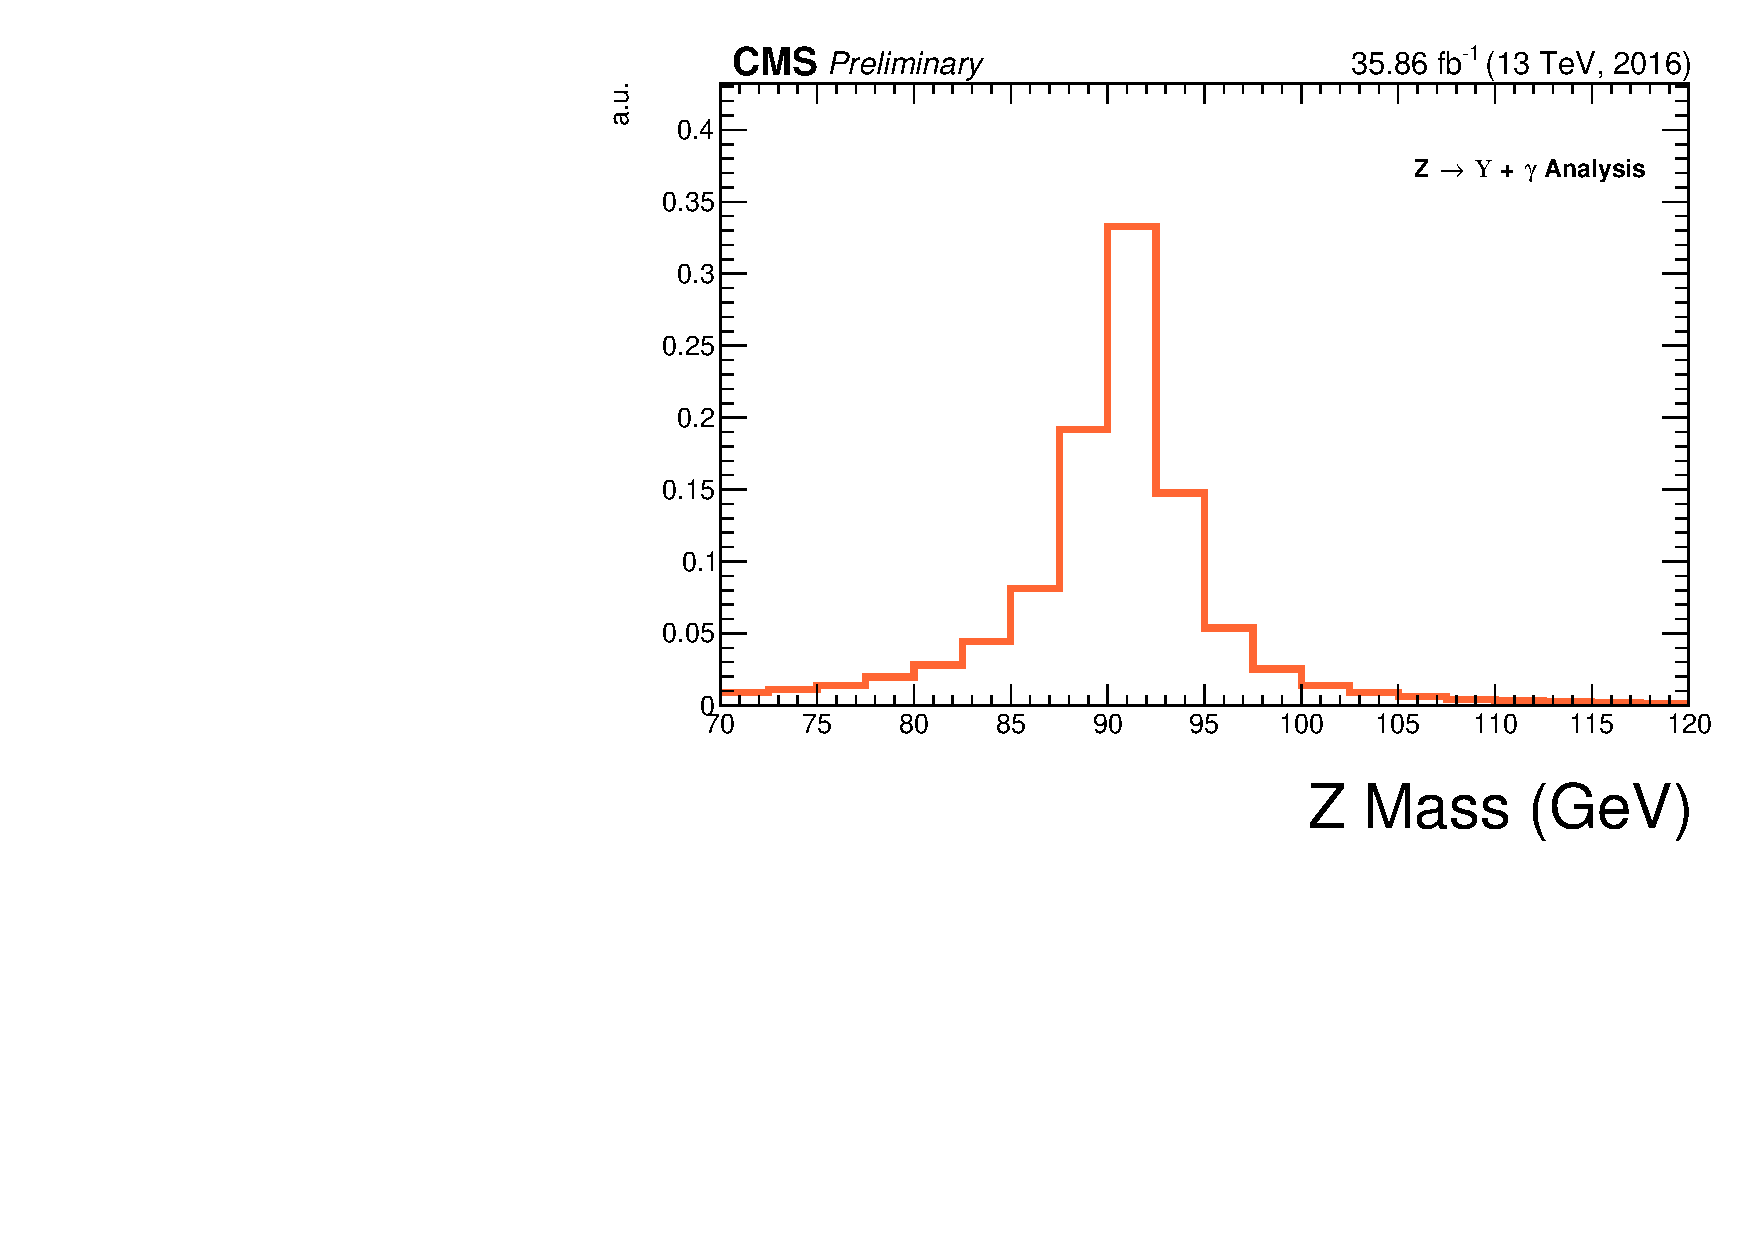
\includegraphics[width=0.25\textwidth]{figures/outputPlots/ZtoUpsilon_Cat0_ZZZZZ/mc/unpolarized/h_Gen_Z_Mass}
%\hspace*{1.cm}
\end{center}%\vspace*{-.5cm}
\caption{Generator level distributions of main variables for $H\rightarrow  \Upsilon(1S,2S,3S) + \gamma$ : Transverse momenta of the leading/trailing $\PT$ muon and the photon, pseudorapidity ($\eta$) and $\phi$ of the muons and the photon, distances $\Delta R$ between the two muons and between the muons and the photon.All the distributions shown in the figure are normalized to the unity of area.}
\label{fig:MC_HtoUpsilon_Cat0}
\end{figure}



% \clearpage
%%%%%%%%%%%%%%%%%%%%%%%%%%%%%%%%%%%%%

\section{Event selection}
\label{sec:selection}

The event selection is divided in two steps. At first, a set of cuts related to trigger and physics object (muons and photons) selection is applied. High level physics objects at CMS are reconstructed based of the Particle Flow (PF) algorithm \cite{PF_paper_2016}. This selection is called, within this analysis, Group I. 

For the events that pass the Group I selection, another set of cuts is applied, this time focusing on kinematical (phase space) event selection, in order to enhance the signal to background ratio. This later set is called, within this analysis, Group II. After full selection, three exclusive categories are defined, based on the photon's $\eta$ region and its energy spread shape within the ECAL cells (R9).

% It was a deliberated choice to apply on this analysis the same event selection of the $H/Z \rightarrow J/\psi + \gamma$  with 2016 data. Full documentation on this analysis can be found at \cite{CMS_jpsi_analysis}. Since the two analyses are similar, not only in final state, but also on the kind of intermediate meson ($\Upsilon$ or $J/\psi$) and energy scale, this choice was taken in order to keep the compatibility of the two studies. The only difference in the event selection is the dimuon mass window, which was changed to a suitable cut for a $\Upsilon$ selection.  

After the full selection, a background and signal modeling process is applied, based on the invariant mass distributions, which will be explained in the next section.


%%%%%%%%%%%%%%%%%%%%%%%%%%%%%%%%%%%%%%%%%%%%%%%%%%%%%%%%%%%%%%%%%%%%%%%%%%%%%%%%%%%%%%%%%%%%%%%%%%%%%%%%%%%%%%%%%%%%%%%%
%%%%%%%%%%%%%%%%%%%%%%%%%%%%%%%%%%%%%%%%%%%%%%%%%%%%%%%%%%%%%%%%%%%%%%%%%%%%%%%%%%%%%%%%%%%%%%%%%%%%%%%%%%%%%%%%%%%%%%%%
%%%%%%%%%%%%%%%%%%%%%%%%%%%%%%%%%%%%%%%%%%%%%%%%%%%%%%%%%%%%%%%%%%%%%%%%%%%%%%%%%%%%%%%%%%%%%%%%%%%%%%%%%%%%%%%%%%%%%%%%
%%%%%%%%%%%%%%%%%%%%%%%%%%%%%%%%%%%%%%%%%%%%%%%%%%%%%%%%%%%%%%%%%%%%%%%%%%%%%%%%%%%%%%%%%%%%%%%%%%%%%%%%%%%%%%%%%%%%%%%%
%%%%%%%%%%%%%%%%%%%%%%%%%%%%%%%%%%%%%%%%%%%%%%%%%%%%%%%%%%%%%%%%%%%%%%%%%%%%%%%%%%%%%%%%%%%%%%%%%%%%%%%%%%%%%%%%%%%%%%%%
%%%%%%%%%%%%%%%%%%%%%%%%%%%%%%%%%%%%%%%%%%%%%%%%%%%%%%%%%%%%%%%%%%%%%%%%%%%%%%%%%%%%%%%%%%%%%%%%%%%%%%%%%%%%%%%%%%%%%%%%
%%%%%%%%%%%%%%%%%%%%%%%%%%%%%%%%%%%%%%%%%%%%%%%%%%%%%%%%%%%%%%%%%%%%%%%%%%%%%%%%%%%%%%%%%%%%%%%%%%%%%%%%%%%%%%%%%%%%%%%%
%%%%%%%%%%%%%%%%%%%%%%%%%%%%%%%%%%%%%%%%%%%%%%%%%%%%%%%%%%%%%%%%%%%%%%%%%%%%%%%%%%%%%%%%%%%%%%%%%%%%%%%%%%%%%%%%%%%%%%%%
%%%%%%%%%%%%%%%%%%%%%%%%%%%%%%%%%%%%%%%%%%%%%%%%%%%%%%%%%%%%%%%%%%%%%%%%%%%%%%%%%%%%%%%%%%%%%%%%%%%%%%%%%%%%%%%%%%%%%%%%
%%%%%%%%%%%%%%%%%%%%%%%%%%%%%%%%%%%%%%%%%%%%%%%%%%%%%%%%%%%%%%%%%%%%%%%%%%%%%%%%%%%%%%%%%%%%%%%%%%%%%%%%%%%%%%%%%%%%%%%%
%%%%%%%%%%%%%%%%%%%%%%%%%%%%%%%%%%%%%%%%%%%%%%%%%%%%%%%%%%%%%%%%%%%%%%%%%%%%%%%%%%%%%%%%%%%%%%%%%%%%%%%%%%%%%%%%%%%%%%%%
%%%%%%%%%%%%%%%%%%%%%%%%%%%%%%%%%%%%%%%%%%%%%%%%%%%%%%%%%%%%%%%%%%%%%%%%%%%%%%%%%%%%%%%%%%%%%%%%%%%%%%%%%%%%%%%%%%%%%%%%
%%%%%%%%%%%%%%%%%%%%%%%%%%%%%%%%%%%%%%%%%%%%%%%%%%%%%%%%%%%%%%%%%%%%%%%%%%%%%%%%%%%%%%%%%%%%%%%%%%%%%%%%%%%%%%%%%%%%%%%%
%
% _______  ______    _______  __   __  _______    ___  
%|       ||    _ |  |       ||  | |  ||       |  |   | 
%|    ___||   | ||  |   _   ||  | |  ||    _  |  |   | 
%|   | __ |   |_||_ |  | |  ||  |_|  ||   |_| |  |   | 
%|   ||  ||    __  ||  |_|  ||       ||    ___|  |   | 
%|   |_| ||   |  | ||       ||       ||   |      |   | 
%|_______||___|  |_||_______||_______||___|      |___| 
%
%%%%%%%%%%%%%%%%%%%%%%%%%%%%%%%%%%%%%%%%%%%%%%%%%%%%%%%%%%%%%%%%%%%%%%%%%%%%%%%%%%%%%%%%%%%%%%%%%%%%%%%%%%%%%%%%%%%%%%%%
%%%%%%%%%%%%%%%%%%%%%%%%%%%%%%%%%%%%%%%%%%%%%%%%%%%%%%%%%%%%%%%%%%%%%%%%%%%%%%%%%%%%%%%%%%%%%%%%%%%%%%%%%%%%%%%%%%%%%%%%
%%%%%%%%%%%%%%%%%%%%%%%%%%%%%%%%%%%%%%%%%%%%%%%%%%%%%%%%%%%%%%%%%%%%%%%%%%%%%%%%%%%%%%%%%%%%%%%%%%%%%%%%%%%%%%%%%%%%%%%%
%%%%%%%%%%%%%%%%%%%%%%%%%%%%%%%%%%%%%%%%%%%%%%%%%%%%%%%%%%%%%%%%%%%%%%%%%%%%%%%%%%%%%%%%%%%%%%%%%%%%%%%%%%%%%%%%%%%%%%%%
%%%%%%%%%%%%%%%%%%%%%%%%%%%%%%%%%%%%%%%%%%%%%%%%%%%%%%%%%%%%%%%%%%%%%%%%%%%%%%%%%%%%%%%%%%%%%%%%%%%%%%%%%%%%%%%%%%%%%%%%
%%%%%%%%%%%%%%%%%%%%%%%%%%%%%%%%%%%%%%%%%%%%%%%%%%%%%%%%%%%%%%%%%%%%%%%%%%%%%%%%%%%%%%%%%%%%%%%%%%%%%%%%%%%%%%%%%%%%%%%%
%%%%%%%%%%%%%%%%%%%%%%%%%%%%%%%%%%%%%%%%%%%%%%%%%%%%%%%%%%%%%%%%%%%%%%%%%%%%%%%%%%%%%%%%%%%%%%%%%%%%%%%%%%%%%%%%%%%%%%%%
%%%%%%%%%%%%%%%%%%%%%%%%%%%%%%%%%%%%%%%%%%%%%%%%%%%%%%%%%%%%%%%%%%%%%%%%%%%%%%%%%%%%%%%%%%%%%%%%%%%%%%%%%%%%%%%%%%%%%%%%
%%%%%%%%%%%%%%%%%%%%%%%%%%%%%%%%%%%%%%%%%%%%%%%%%%%%%%%%%%%%%%%%%%%%%%%%%%%%%%%%%%%%%%%%%%%%%%%%%%%%%%%%%%%%%%%%%%%%%%%%
%%%%%%%%%%%%%%%%%%%%%%%%%%%%%%%%%%%%%%%%%%%%%%%%%%%%%%%%%%%%%%%%%%%%%%%%%%%%%%%%%%%%%%%%%%%%%%%%%%%%%%%%%%%%%%%%%%%%%%%%
%%%%%%%%%%%%%%%%%%%%%%%%%%%%%%%%%%%%%%%%%%%%%%%%%%%%%%%%%%%%%%%%%%%%%%%%%%%%%%%%%%%%%%%%%%%%%%%%%%%%%%%%%%%%%%%%%%%%%%%%
%%%%%%%%%%%%%%%%%%%%%%%%%%%%%%%%%%%%%%%%%%%%%%%%%%%%%%%%%%%%%%%%%%%%%%%%%%%%%%%%%%%%%%%%%%%%%%%%%%%%%%%%%%%%%%%%%%%%%%%%
%%%%%%%%%%%%%%%%%%%%%%%%%%%%%%%%%%%%%%%%%%%%%%%%%%%%%%%%%%%%%%%%%%%%%%%%%%%%%%%%%%%%%%%%%%%%%%%%%%%%%%%%%%%%%%%%%%%%%%%%
%%%%%%%%%%%%%%%%%%%%%%%%%%%%%%%%%%%%%%%%%%%%%%%%%%%%%%%%%%%%%%%%%%%%%%%%%%%%%%%%%%%%%%%%%%%%%%%%%%%%%%%%%%%%%%%%%%%%%%%%
%%%%%%%%%%%%%%%%%%%%%%%%%%%%%%%%%%%%%%%%%%%%%%%%%%%%%%%%%%%%%%%%%%%%%%%%%%%%%%%%%%%%%%%%%%%%%%%%%%%%%%%%%%%%%%%%%%%%%%%%

\section{Trigger and physics object selection (Group I)}

\subsection{Trigger}
\label{sec:trigger}
% The trigger used to select events, At hardware level (called L1), it is seeded by at least one muon with $p_{T} > 5$ GeV (transverse momentum with respect to the proton beam line)  and a isolated E/$\gamma$ with $p_{T} > 18$ GeV. At software level (HLT), it is activated by at least one muon with $p_{T} > 17$ GeV and a Photon of $p_{T} > 30$ GeV.

In this study, the same trigger requirements are applied to both data and simulated samples. For the first trigger level (L1), events are selected if they present at least one muon with transverse momentum greater than 5 GeV and an isolated~\footnote{The concept of isolation will be detailed later, but in summary, it means a object which has very small activity (above a certain threshold of energy/momentum) around it. In hadron-hadron collider, isolation is a characteristics of hard interactions.} photon or electron with transverse momentum greater than 18 GeV (at L1, there is no differentiation between photons and electrons). At the software level of the trigger system (HLT), the events are required to have at least one muon with transverse momentum greater than 17 GeV and a photon with transverse momentum greater than 30 GeV.

In order to compensate any difference in the trigger performance between simulated and data samples, for every selected MC a proper scale factor is applied, based on the the \PT of the reconstructed muon and photon. Considering the similarity of this analysis with the $H/Z \rightarrow J/\psi + \gamma$ analysis~\cite{papper_jpsi}, not only in therm of data samples, but also for triggering and physics object selection, the same scale factors were applied.

\subsection{Muon Identification}
\label{sec:muon_id}
% After trigger selection, the same muon selection of the $H \rightarrow ZZ^{*} \rightarrow 4l$ is applied \cite{CMS_higgs_zz_4l}. This is the same approach used by the $H/Z \rightarrow J/\psi + \gamma$ analysis. 

Ahead of any selection, a standard CMS "Ghost Cleaning" procedure is applied to all reconstructed muons in order to avoid that a single physical muon is reconstructed as two or more. For this procedure, reconstructed muons sharing 50\% or more segments in the system are arbitrated.

After the cleaning, a muon is chosen when it passes a a two step identification: the \textbf{Loose ID} and the \textbf{Tight ID}. Below the muon identification procedure is summarized .

% One should keep in mind that the naming conventions for these definitions are exclusive for the $H \rightarrow ZZ^{*} \rightarrow 4l$ and, therefore, to this analysis, not corresponding to the Muon-POG definitions. 

For the Loose ID, each muon is required to:
\begin{itemize}
  \item have transverse momentum greater than 5 GeV, in order to cope with Particle Flow requirements;
  \item be within the muon system acceptance: $|\eta| < 2.4$;
  \item to have a three dimensional impact parameter uncertainty smaller than 4;
  \item to have transverse distance smaller than 0.5 cm ($d_{xy} < 0.5$), with respect to the primary vertex (PV);
  \item to have longitudinal distance greater than 1.0 cm ($d_{z} < 1$), with respect to the primary vertex (PV).

  % \item reconstructed as \textbf{Global Muon} or \textbf{Tracker Muon};
  % \item muon tracks only in the muon system are rejected;
  % \item muons with \texttt{muonBestTrackType==2} (standalone) are discarded.
\end{itemize}

Muons reconstructed only in the muon system, without a correspondence with the tracker, are rejected. The last three requirements of the Loose ID are imposed in order to suppress muons from in-flight decays.

The primary vertex itself, is determined as the reconstructed vertex with the biggest sum of $p_T^2$ in the event. This sum is performed, considering all the charged PF candidates clustered by the jet finding algorithms~\cite{Cacciari:2008gp,Cacciari:2011ma} and the MET, which is defined as the $p_T$ vector sum of all the charged and neutral PF candidates associated to that vertex. 

For the Tight ID, muons with transverse momentum $p_{T} < 200$ GeV, are required to have been reconstructed with the Particle Flow (PF) algorithm. If they have $p_{T} > 200$ GeV, they should reconstructed with the Particle Flow (PF) algorithm or satisfy the strict tracker requirements (defined in table~\ref{tab:Tracker_High_pT}).

\begin{table}[h]
    \begin{center}
    \begin{tabular}{l|l}
     % \hline
     \textbf{Requirement}         & \textbf{Technical definition}                 \\
      \hline
      Muon station matching          & Muon is matched to segments           \\
                                     & in at least two stations in the muon system        \\
      \hline                                                          
      Good $\pt$ measurement         & $\frac{\pt}{\sigma_{\pt}} < 0.3$      \\
      \hline
      Vertex compatibility ($x-y$)   & $d_{xy} < 2$~mm                       \\
      \hline
      Vertex compatibility ($z$)     & $d_{z} < 5$~mm                        \\
      \hline
      Pixel hits                     & At least one pixel hit                \\
      \hline
      Tracker hits                   & Hits in at least six tracker layers   \\
      \hline
    \end{tabular}
    \caption{
      Conditions for a muon to pass the strict tracker requirements.
      }
    \label{tab:Tracker_High_pT}
    \end{center}
\end{table}


To mitigate spurious signal in the detector that would mimic a muon, the leading muon (the one with highest $p_T$) is required to be isolated within a cone of radious $\Delta R = \sqrt{\smash[b]{\Delta \eta}^2 + {\Delta \phi}^2}< 0.3$ in the $\eta - \phi$ plane. The isolation is evaluated in terms of ${\cal I}^{\mu} < 0.35$, defined as:


\begin{equation}
\label{eqn:pfiso}
{\cal I}^{\mu} \equiv \Big( \sum \PT^\text{charged} +
                                 \max\left[ 0, \sum \PT^\text{neutral}
                                 +
                                  \sum \PT^{\cPgg}
                                 - \PT^\mathrm{PU}(\mu) \right] \Big)
                                 / \PT^{\mu}.
\end{equation}


The $\sum \PT^\text{charged}$ is the scalar sum of the transverse momenta of charged hadrons originating from the chosen primary vertex of the event. The $\sum \PT^\text{neutral}$ and $\sum \PT^{\cPgg}$ are the scalar sums of the transverse momenta for neutral hadrons and photons, respectively.  Since the isolation variable is particularly sensitive to energy deposits from pileup interactions, a $\PT^\text{PU}(\mu)$ contribution is subtracted, where $\PT^\mathrm{PU}(\PGm) \equiv 0.5 \times \sum_i \PT^{\mathrm{PU}, i}$, where $i$ runs over the momenta of the charged hadron PF candidates not originating from the primary vertex, and the factor of 0.5 corrects for the different fraction of charged and neutral particles in the cone. 


% The last requirement over the selected muons is that the leading muon should be relatively isolated, over the Particle Flow ($\text{RelPFiso}(\Delta R = 0.3) < 0.35$).


% \begin{equation}
% \text{RelPFiso} = \frac{\sum^\text{charged had.} \pt + \max(\sum^\text{neutral had.} \ET 
% + \sum^\text{photon} \ET - \Delta \beta, 0)}{\pt^\text{lepton}}
% \label{eqn:mupfiso}
% \end{equation}

% The $\Delta\beta$, defined as $\Delta\beta = \frac{1}{2} \sum^\text{charged had.}_\text{PU} \pt$ gives an estimate of the pile-up contribution.  



One should keep in mind that this muon identification is the same as the one used by the $H \rightarrow ZZ^{*} \rightarrow 4l$~\cite{higgs_zz_4l_papper}. This was done in order to keep in phase with other Higgs analysis inside the collaboration. After the muon identification, an appropriate scale factor is applied to the MC events based on the leading muon \PT and $\eta$, in order to correct any possible discrepancy between data and simulated samples. The scale factors were taken from the $H \rightarrow ZZ^{*} \rightarrow 4l$ analysis.

In order to cope with trigger requirements, the leading muon should have $\PT > 20$ GeV and the trailing muon $\PT > 4$ GeV.


\subsection{Photon Identification}
\label{sec:photon_id}

For the photon identification and selection, standard CMS . The Multivariate (MVA) Photon identification is used with a working point of 90\%, together with a electron veto procedure, to avoid misidentification of electrons as photons. Kinematically, the photons are requested to have transverse energy, with respect to the beam line, $E_{T} > 33$ GeV and reconstructed within the CMS acceptance for photons $|\eta_{SC}| < 2.5$\footnote{SC stands for Super Cluster of the reconstructed photon. It is the set of cell in the Electromagnetic Calorimeter used for the photon observation.}, excluding the Electromagnetic Calorimeter (ECAL) Barrel-Endcap intersections.

The threshold of 33 GeV for the photon transverse energy is driven by the trigger requirements. The selecte photon, per event, is the one with highest $E_{T}$.


\subsection{Kinematical distributions}
\label{sec:kin_plots_group_1}

The selection described so far, is called Group I. The plots shown below are related to selected events after this set. 

Figures \ref{fig:pTMuons_ZtoUpsilon_Cat0} to \ref{fig:phiPhoton_ZtoUpsilon_Cat0} presents the \PT, $\eta$ and $\phi$ distributions for the leading muon, trailing muon and the photon, for the \Z decaying in $\Upsilon(1S,2S,3S)$ + $\gamma$. 

Figures \ref{fig:pTUpsilon_and_Z_ZtoUpsilon_Cat0} to \ref{fig:phiUpsilon_and_Z_ZtoUpsilon_Cat0} presents the \PT, $\eta$ and $\phi$ distributions for reconstructed $\Upsilon(nS)$ ($\mu\mu$ system) and the reconstructed boson ($\mu\mu\gamma$ system).

Figures \ref{fig:deltaR_ZtoUpsilon_Cat0} to \ref{fig:dimuon_mass_ZtoUpsilon_Cat0} presents the $\Delta R = \sqrt{\Delta\eta^2 + \Delta\phi^2}$ between the photon and the muons, the $\Delta R$ distributions between reconstructed dimuon ($\mu\mu$) system and the photon, the absolute value of the $\Delta \phi$ between the leading muon and the photon, the ratio for the transverse momentum of the reconstructed Upsilon and the reconstructed Z mass ($p_{T}^{\mu\mu}/M_{\mu\mu\gamma}$), the ratio for the transverse energy of the reconstructed Photon and the reconstructed Z mass ($E_{T}^{\mu\mu}/M_{\mu\mu\gamma}$) and dimuon mass distribution of the reconstructed $\Upsilon(nS)$.

Figures \ref{fig:pTMuons_HtoUpsilon_Cat0} to \ref{fig:dimuon_mass_HtoUpsilon_Cat0} present the same variables, but for the Higgs decaying in $\Upsilon(1S,2S,3S)$ + $\gamma$ channel.

%CONTROL PLOTS
%%$\pT$ muon distributions for ZtoUpsilon_Cat0
\begin{figure}[!htbp]
\begin{center}
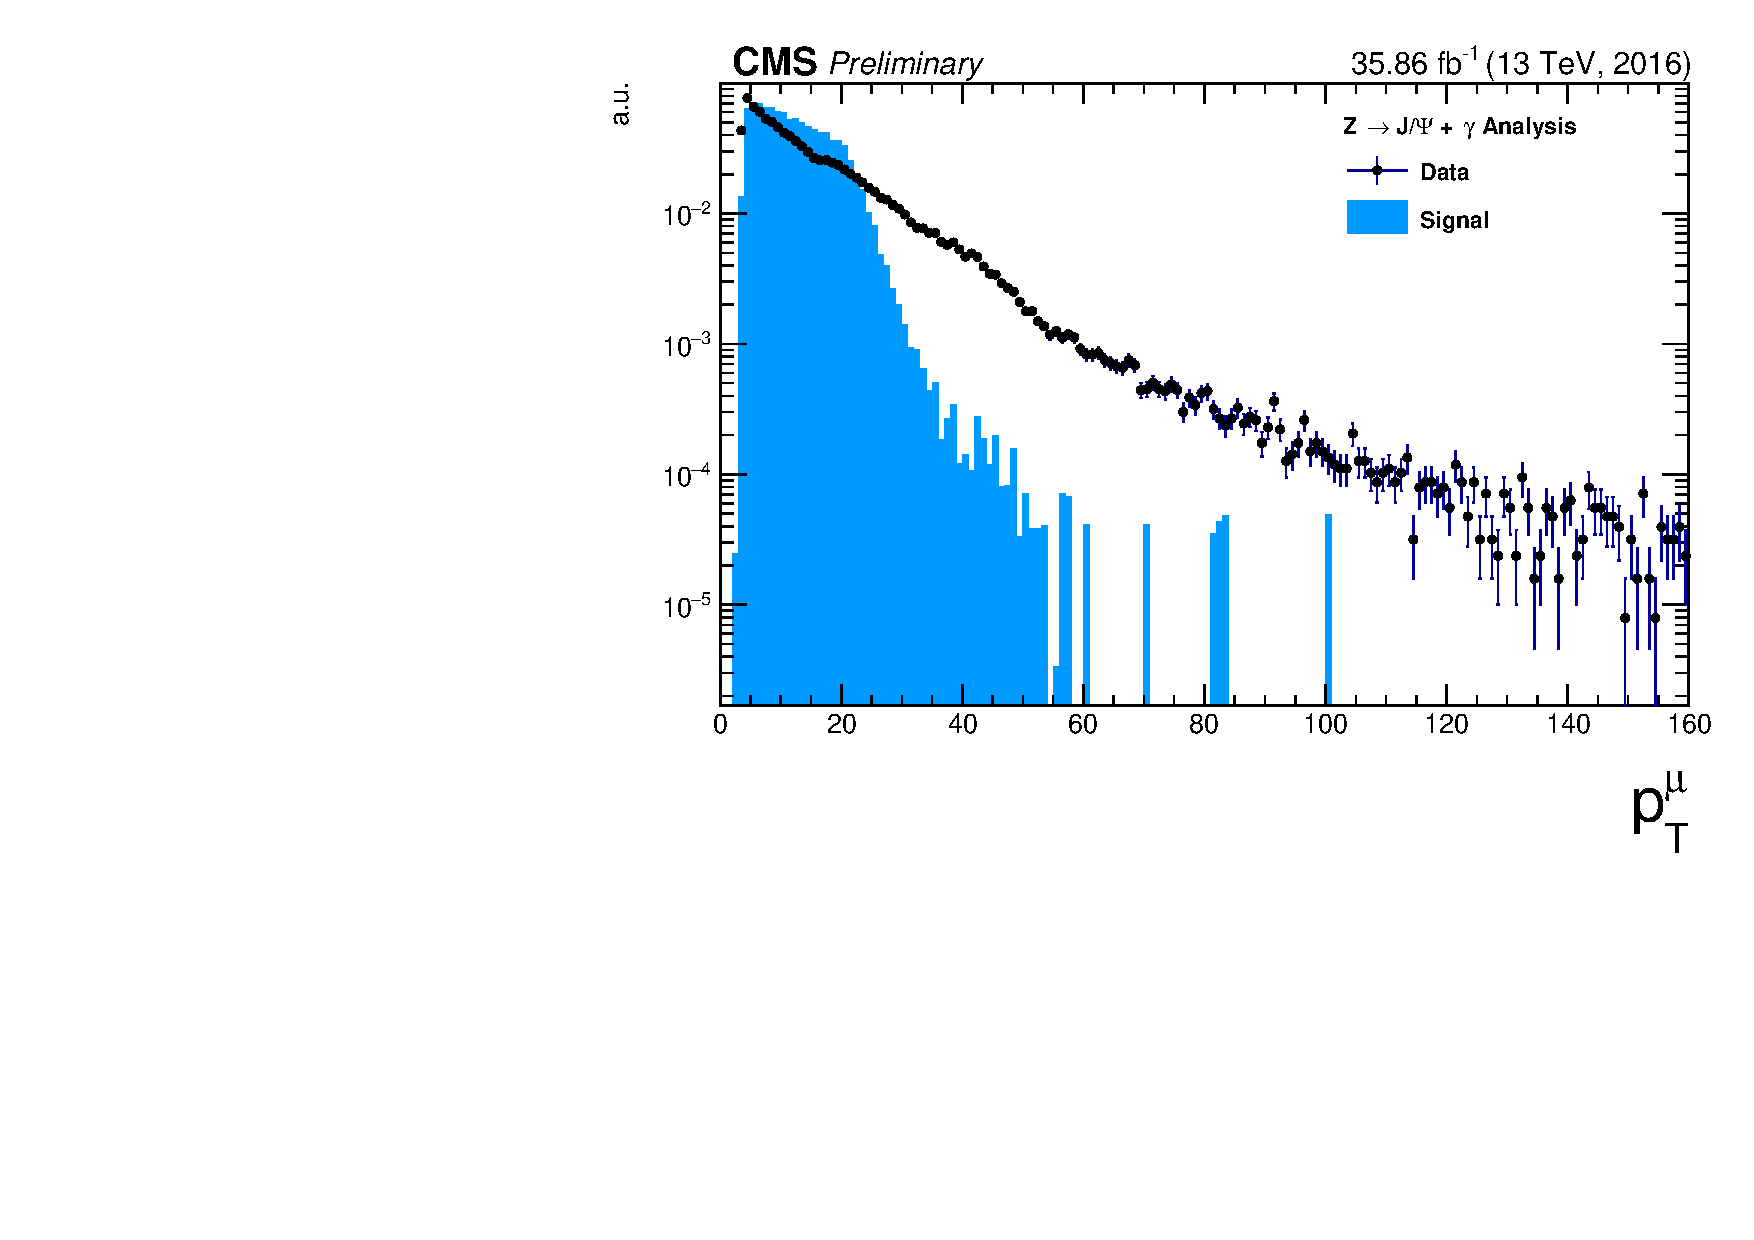
\includegraphics[width=0.45\textwidth]{figures/outputPlots/ZtoUpsilon_Cat0_ZZZZZ/au/data_x_mc/noKinCuts/h_noKin_TrailingMu_pt}\hspace*{1.cm}
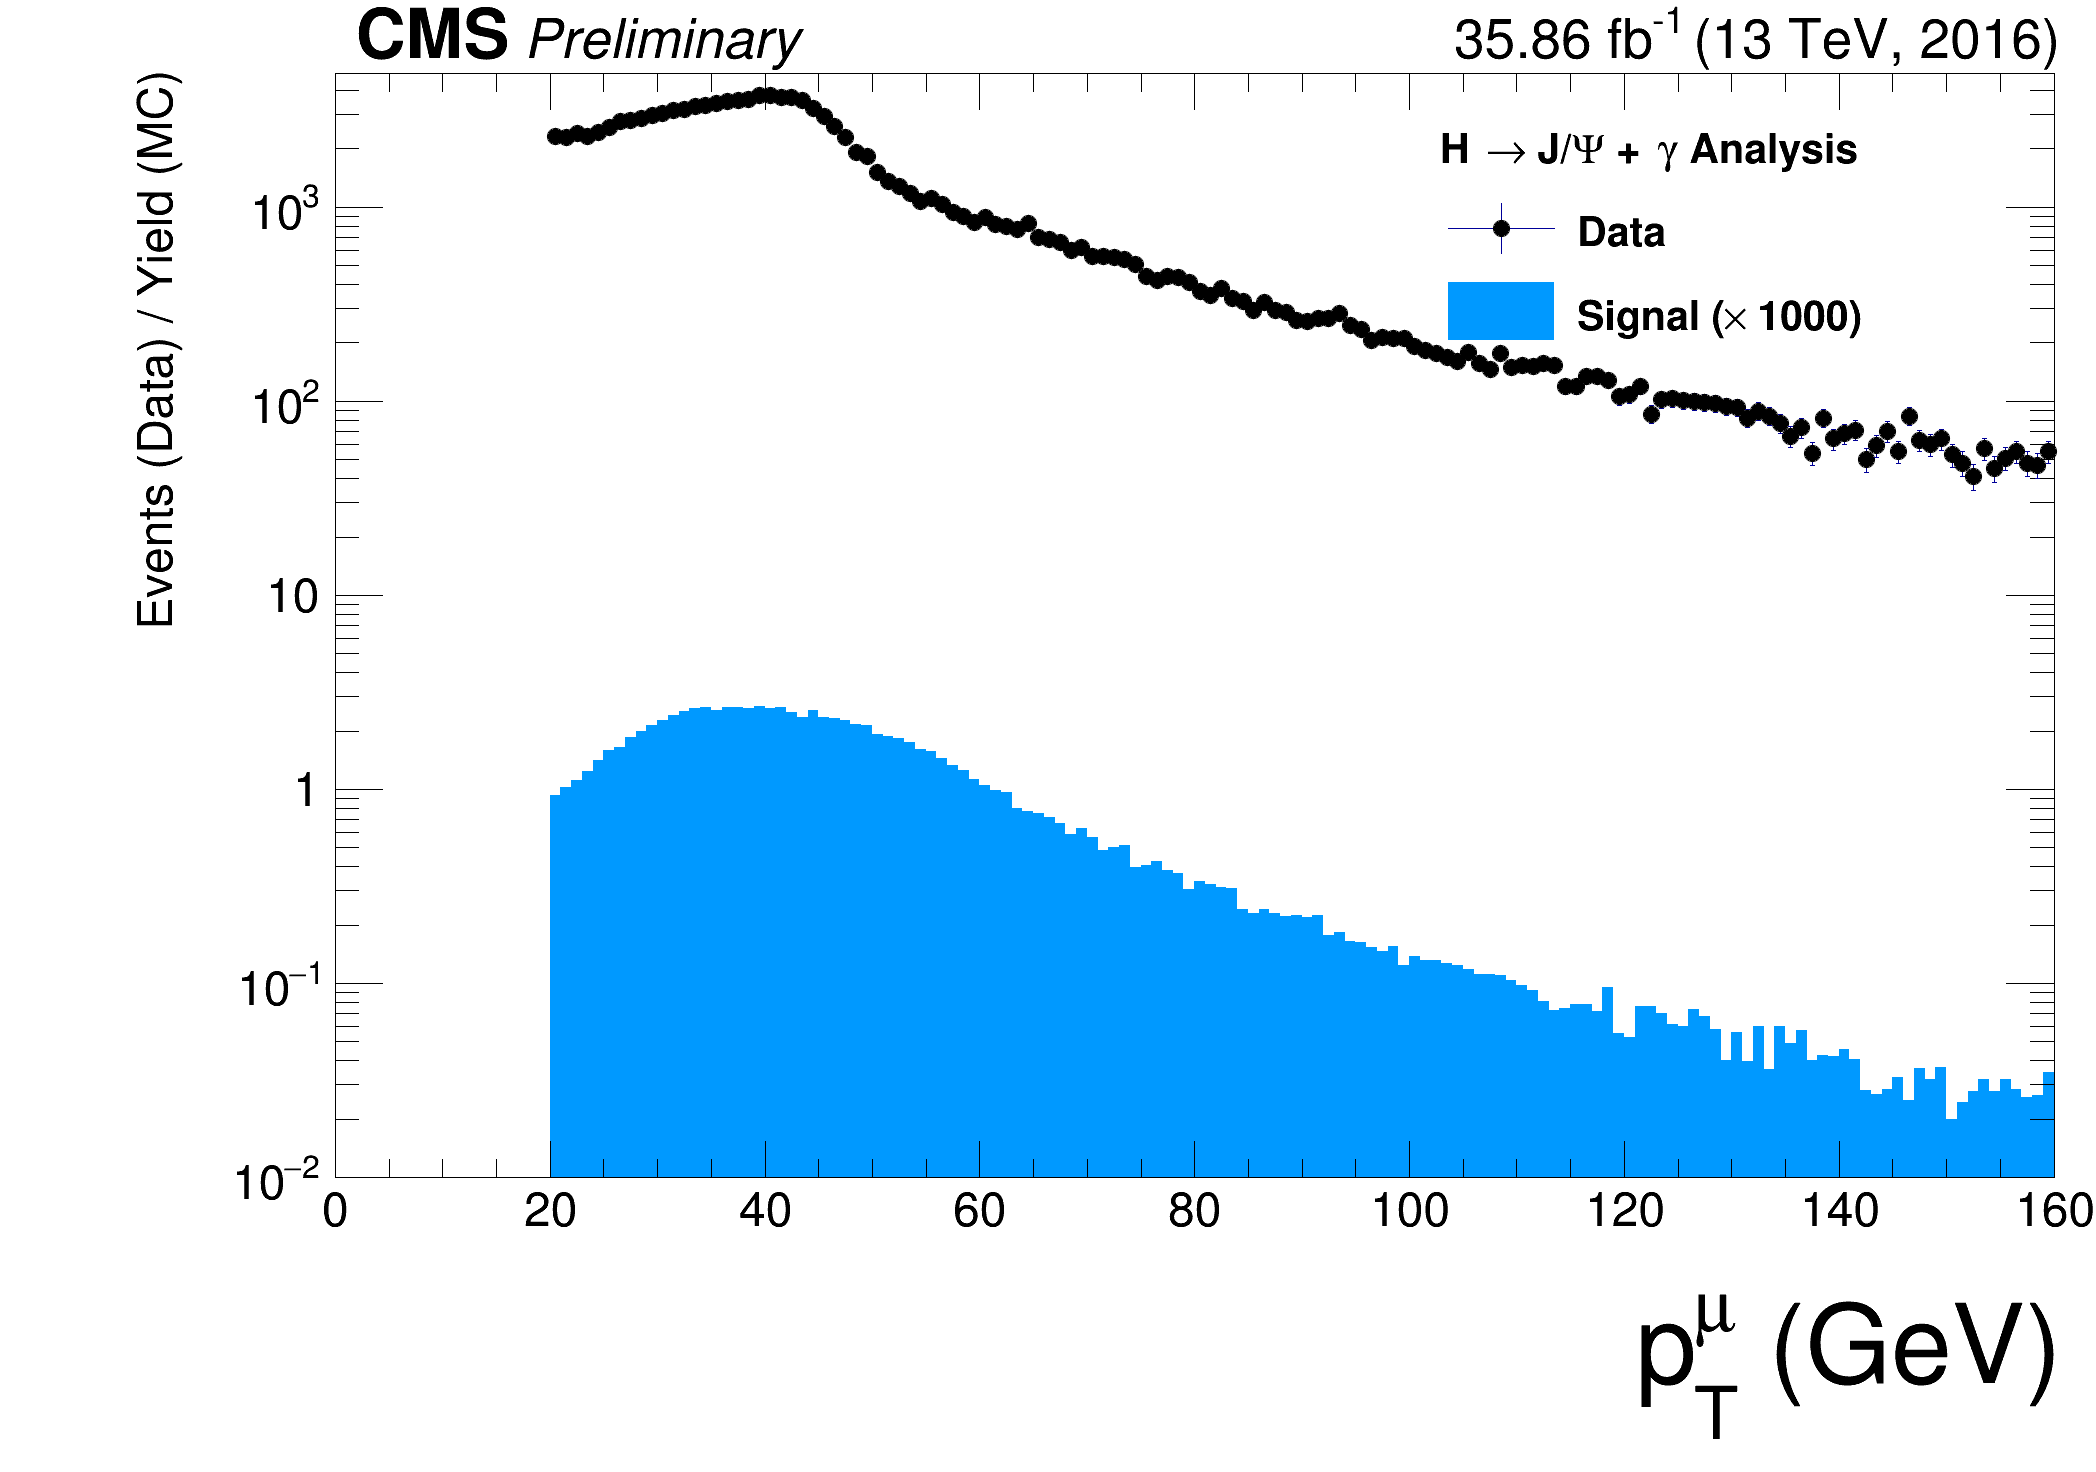
\includegraphics[width=0.45\textwidth]{figures/outputPlots/ZtoUpsilon_Cat0_ZZZZZ/au/data_x_mc/noKinCuts/h_noKin_LeadingMu_pt}
\end{center}\vspace*{-.5cm}
\caption{The \PT muon distributions from data and signal events for \Z decaying in $\Upsilon(1S,2S,3S)$ + $\gamma$ after Group I of selection cuts, where on left are presenting the trailing muons and on right are the leading muons. The plots are normalized to the unit of area.}
\label{fig:pTMuons_ZtoUpsilon_Cat0}
\end{figure}


%%%%%%%$\eta$ muon distributions for ZtoUpsilon_Cat0
\begin{figure}[!htbp]
\begin{center}
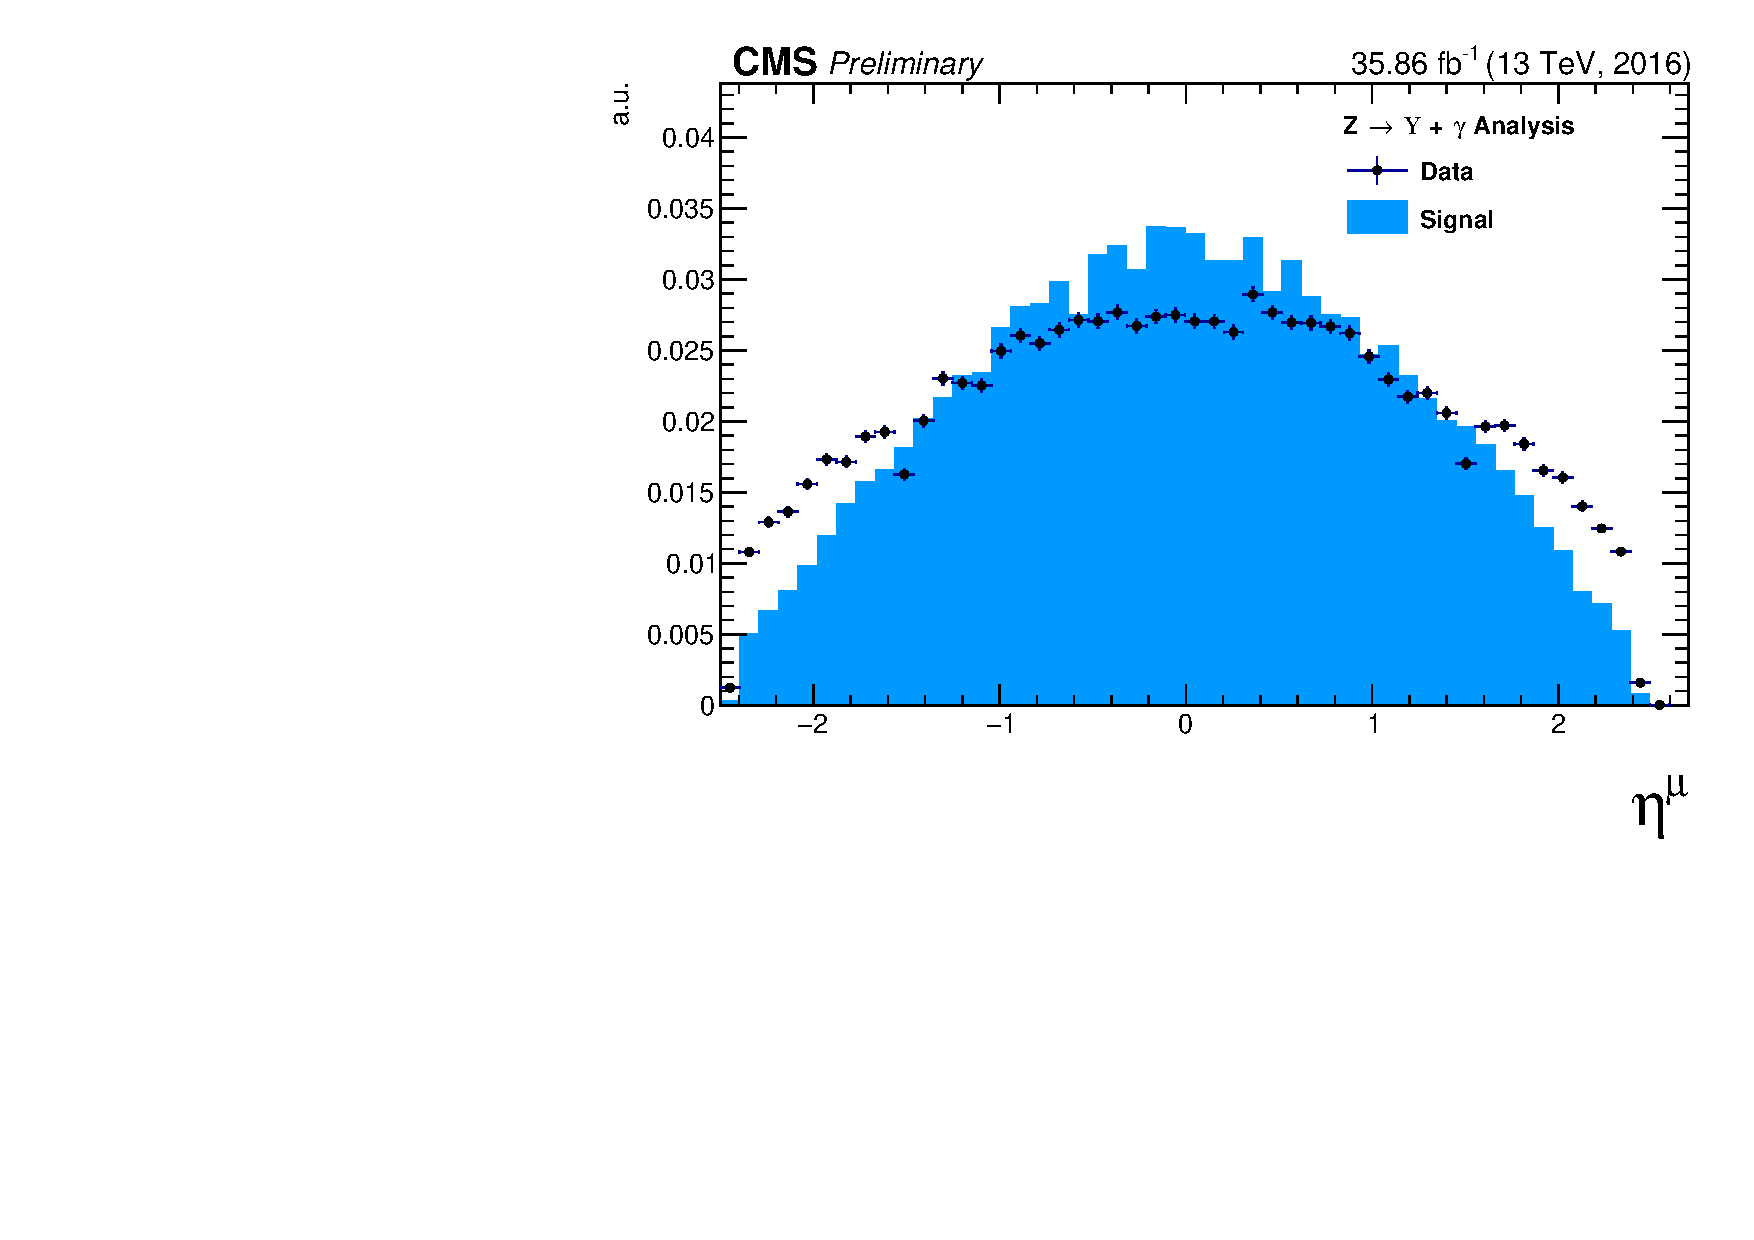
\includegraphics[width=0.45\textwidth]{figures/outputPlots/ZtoUpsilon_Cat0_ZZZZZ/au/data_x_mc/noKinCuts/h_noKin_TrailingMu_eta}\hspace*{1.cm}
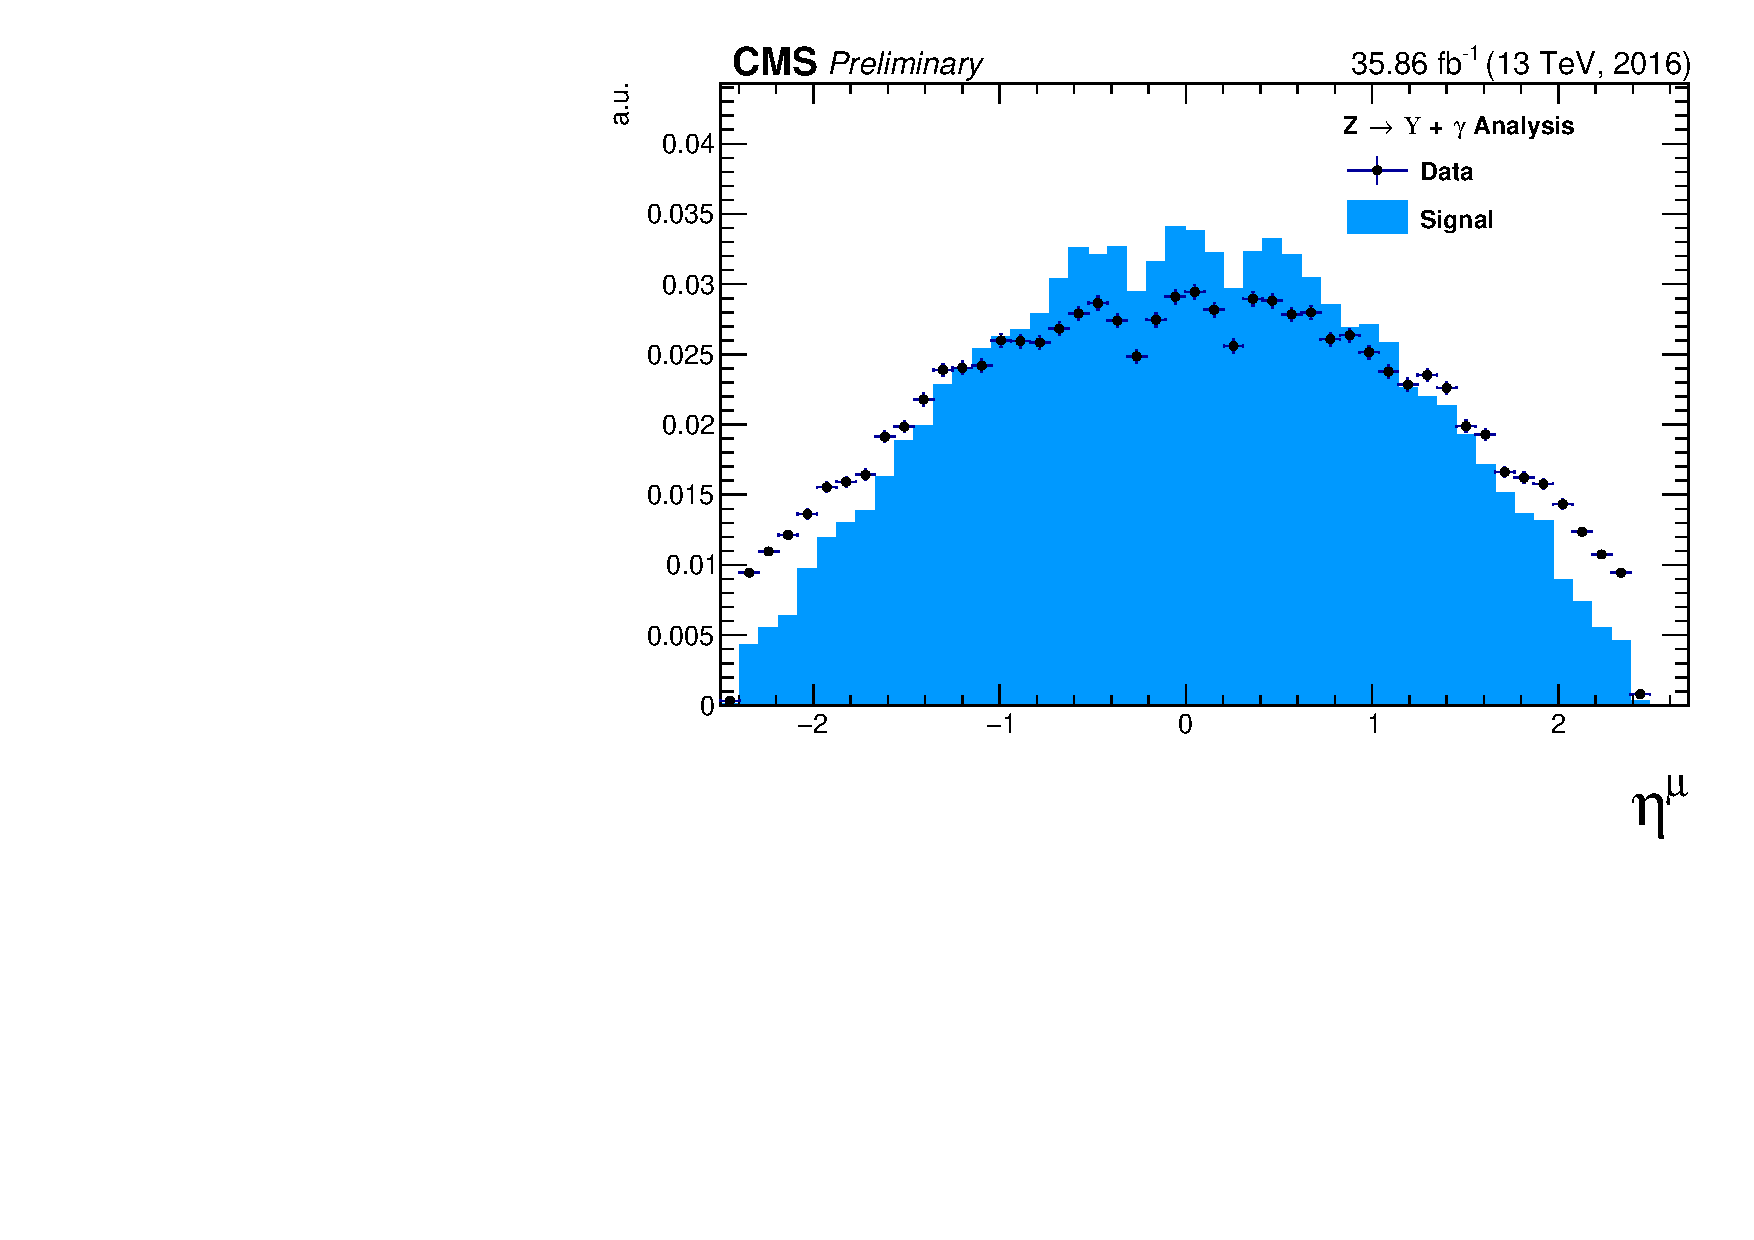
\includegraphics[width=0.45\textwidth]{figures/outputPlots/ZtoUpsilon_Cat0_ZZZZZ/au/data_x_mc/noKinCuts/h_noKin_LeadingMu_eta}
\end{center}\vspace*{-.5cm}
\caption{The $\eta$ muon distributions from data and signal events of \Z decaying in $\Upsilon(1S,2S,3S)$ + $\gamma$ after Group I of selection cuts, where on left are presenting the trailing muons and on right are the leading muons. The plots are normalized to the unit of area.}
\label{fig:etaMuons_ZtoUpsilon_Cat0}
\end{figure}

%%%%%%%%% $\phi$ muon distributions for ZtoUpsilon_Cat0
\begin{figure}[!htbp]
\begin{center}
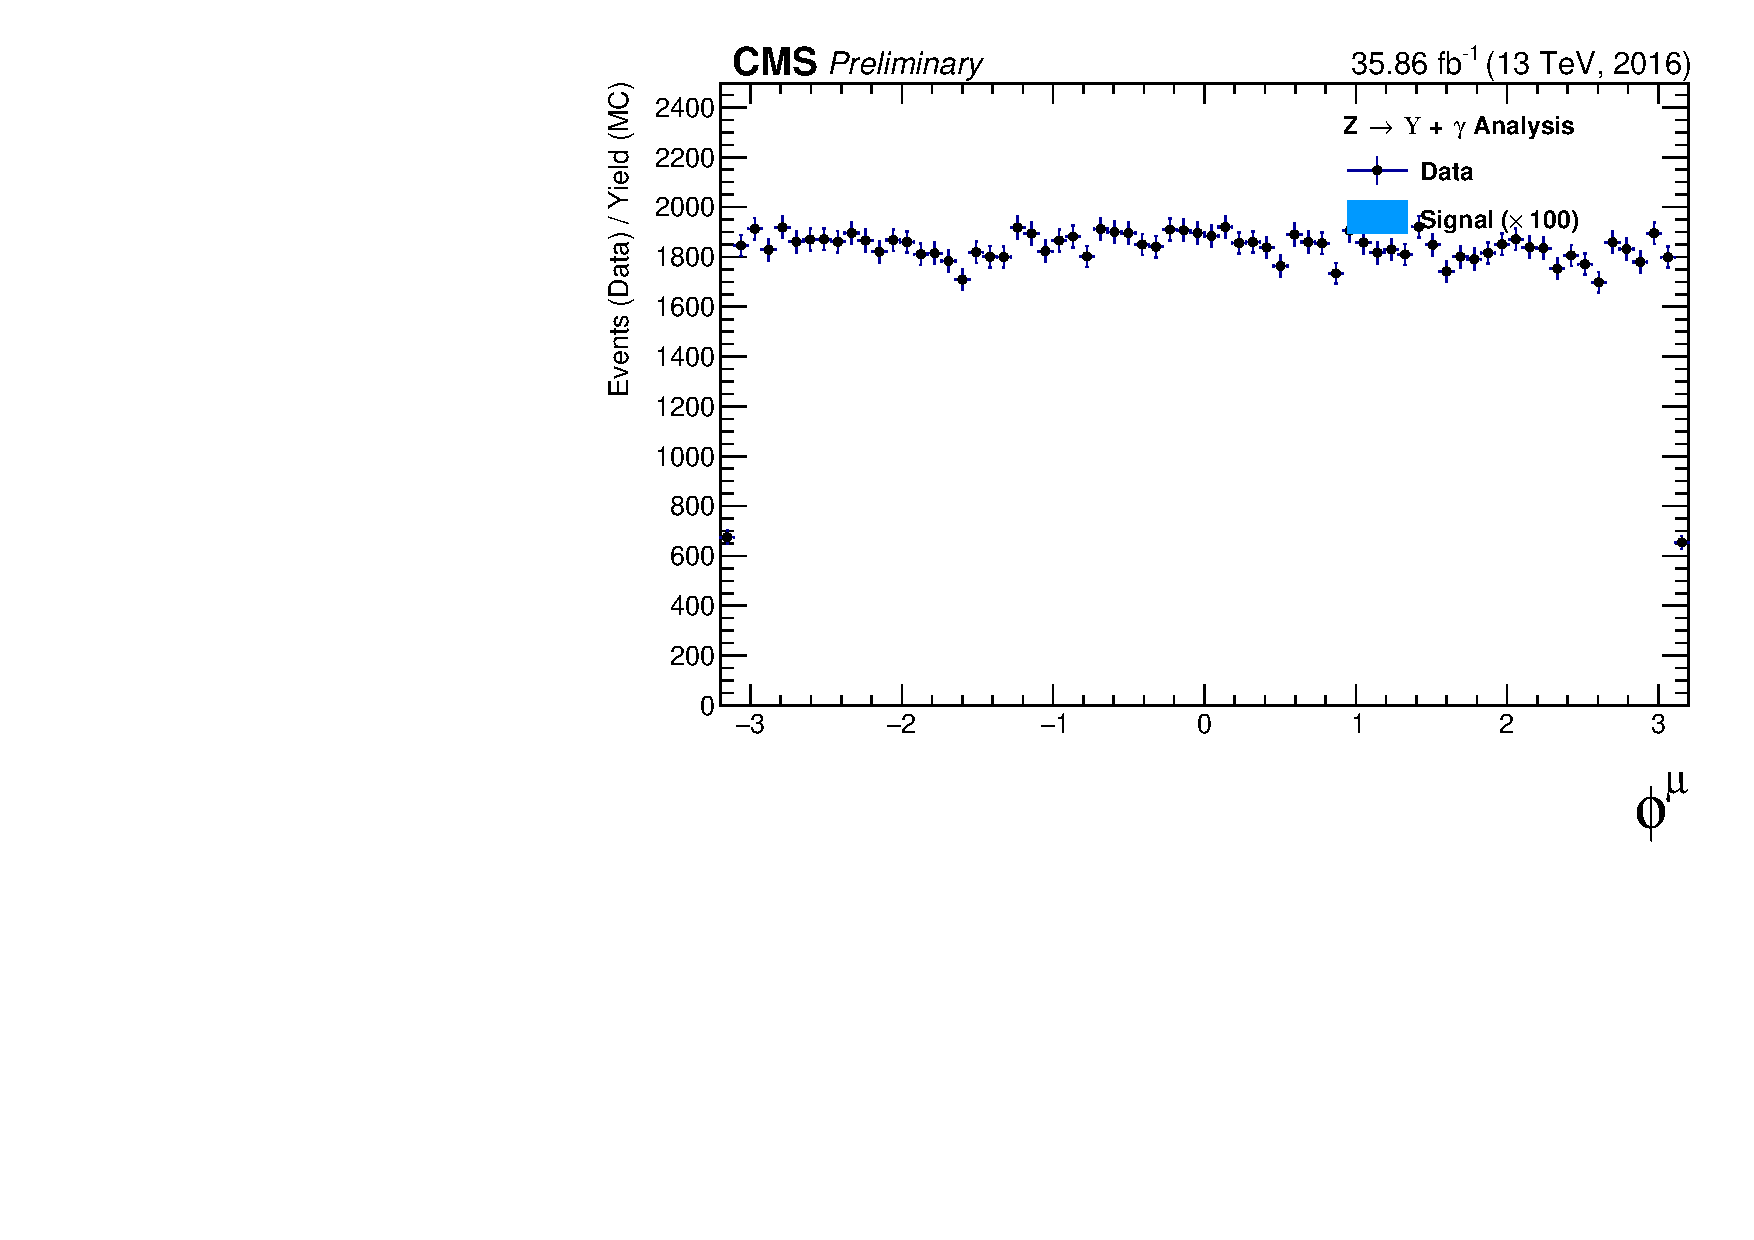
\includegraphics[width=0.45\textwidth]{figures/outputPlots/ZtoUpsilon_Cat0_ZZZZZ/au/data_x_mc/noKinCuts/h_noKin_TrailingMu_phi}\hspace*{1.cm}
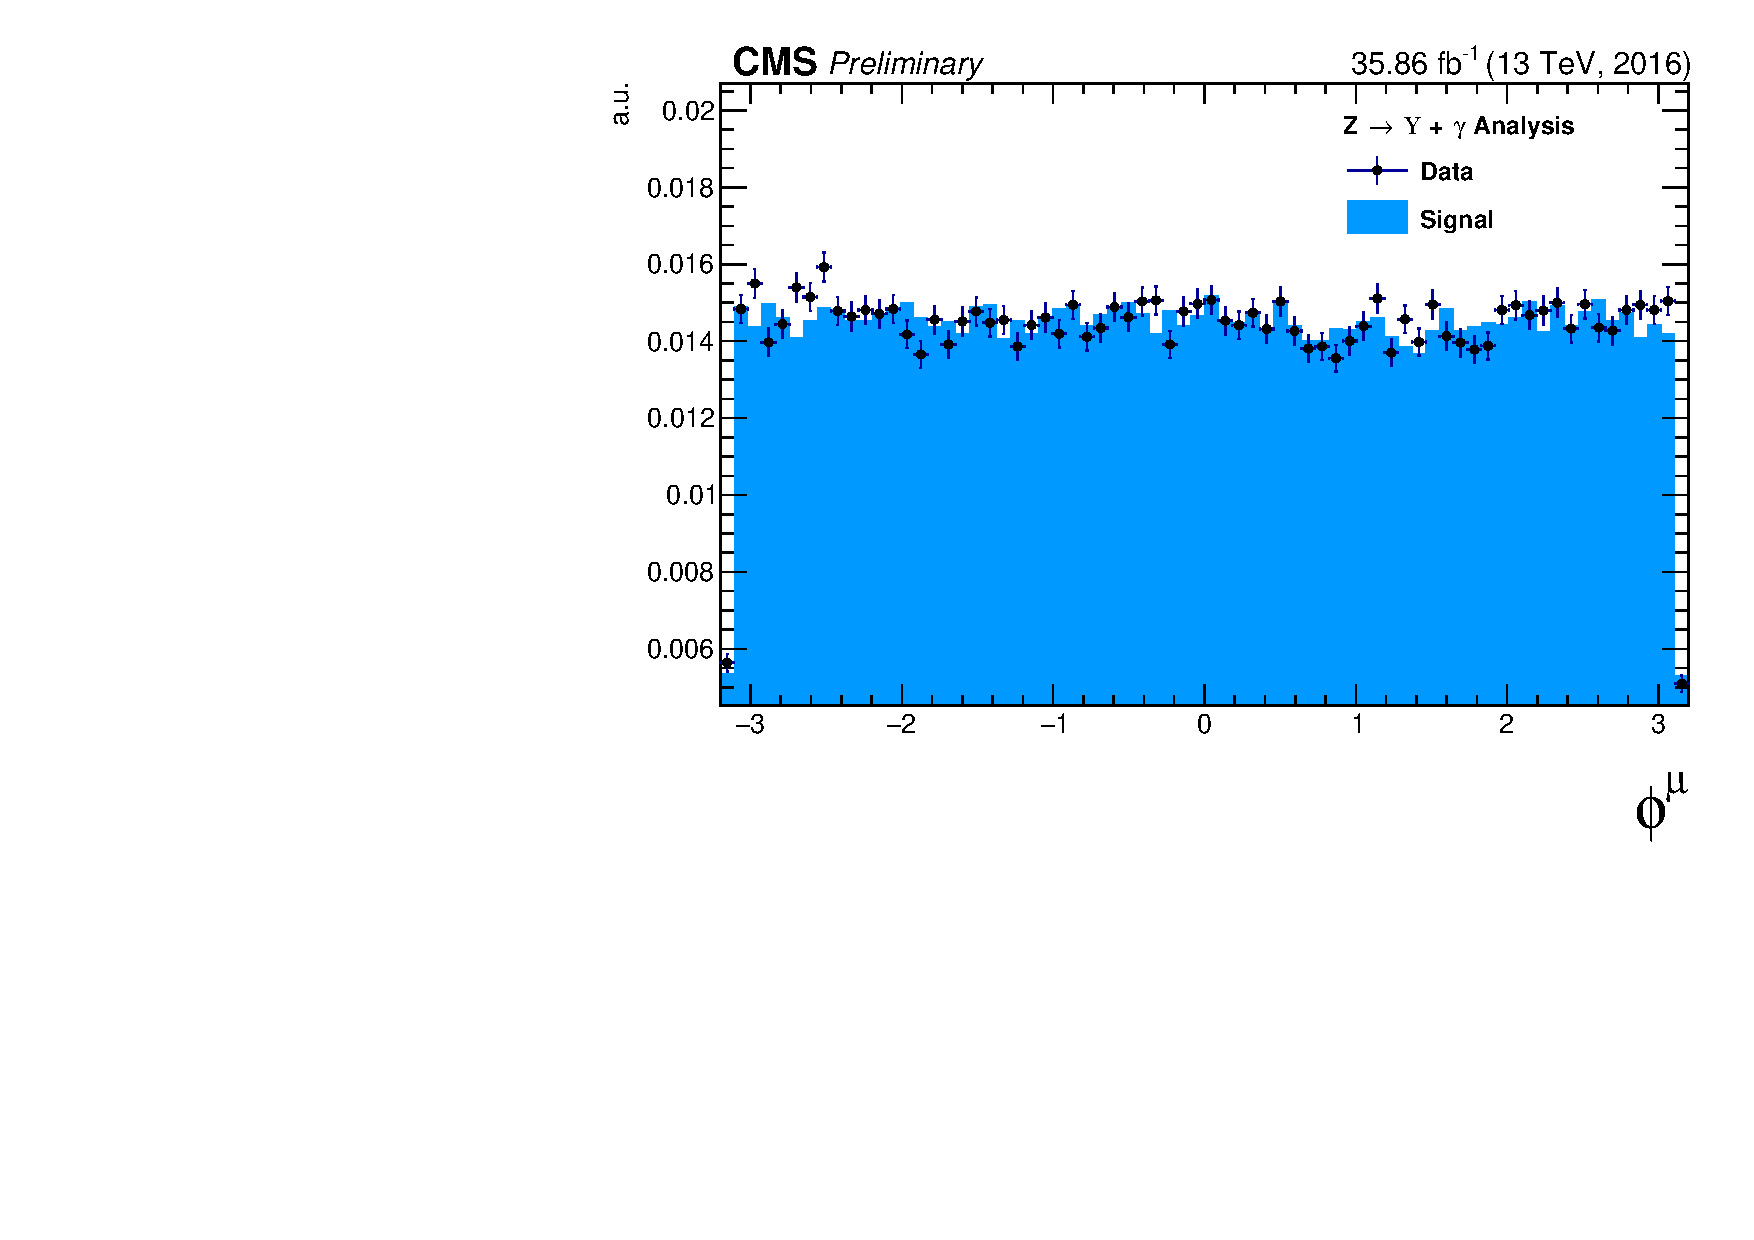
\includegraphics[width=0.45\textwidth]{figures/outputPlots/ZtoUpsilon_Cat0_ZZZZZ/au/data_x_mc/noKinCuts/h_noKin_LeadingMu_phi}
\end{center}\vspace*{-.5cm}
\caption{The $\phi$ muon distributions from data and signal events of \Z decaying in $\Upsilon(1S,2S,3S)$ + $\gamma$ after Group I of selection cuts, where on left are presenting the trailing muons and on right are the leading muons. The plots are normalized to the unit of area.}
\label{fig:phiMuons_ZtoUpsilon_Cat0}
\end{figure}

%%%%%%%%%%%%%

%photon
%%$\pT$ Photon distributions for ZtoUpsilon_Cat0
\begin{figure}[!htbp]
\begin{center}
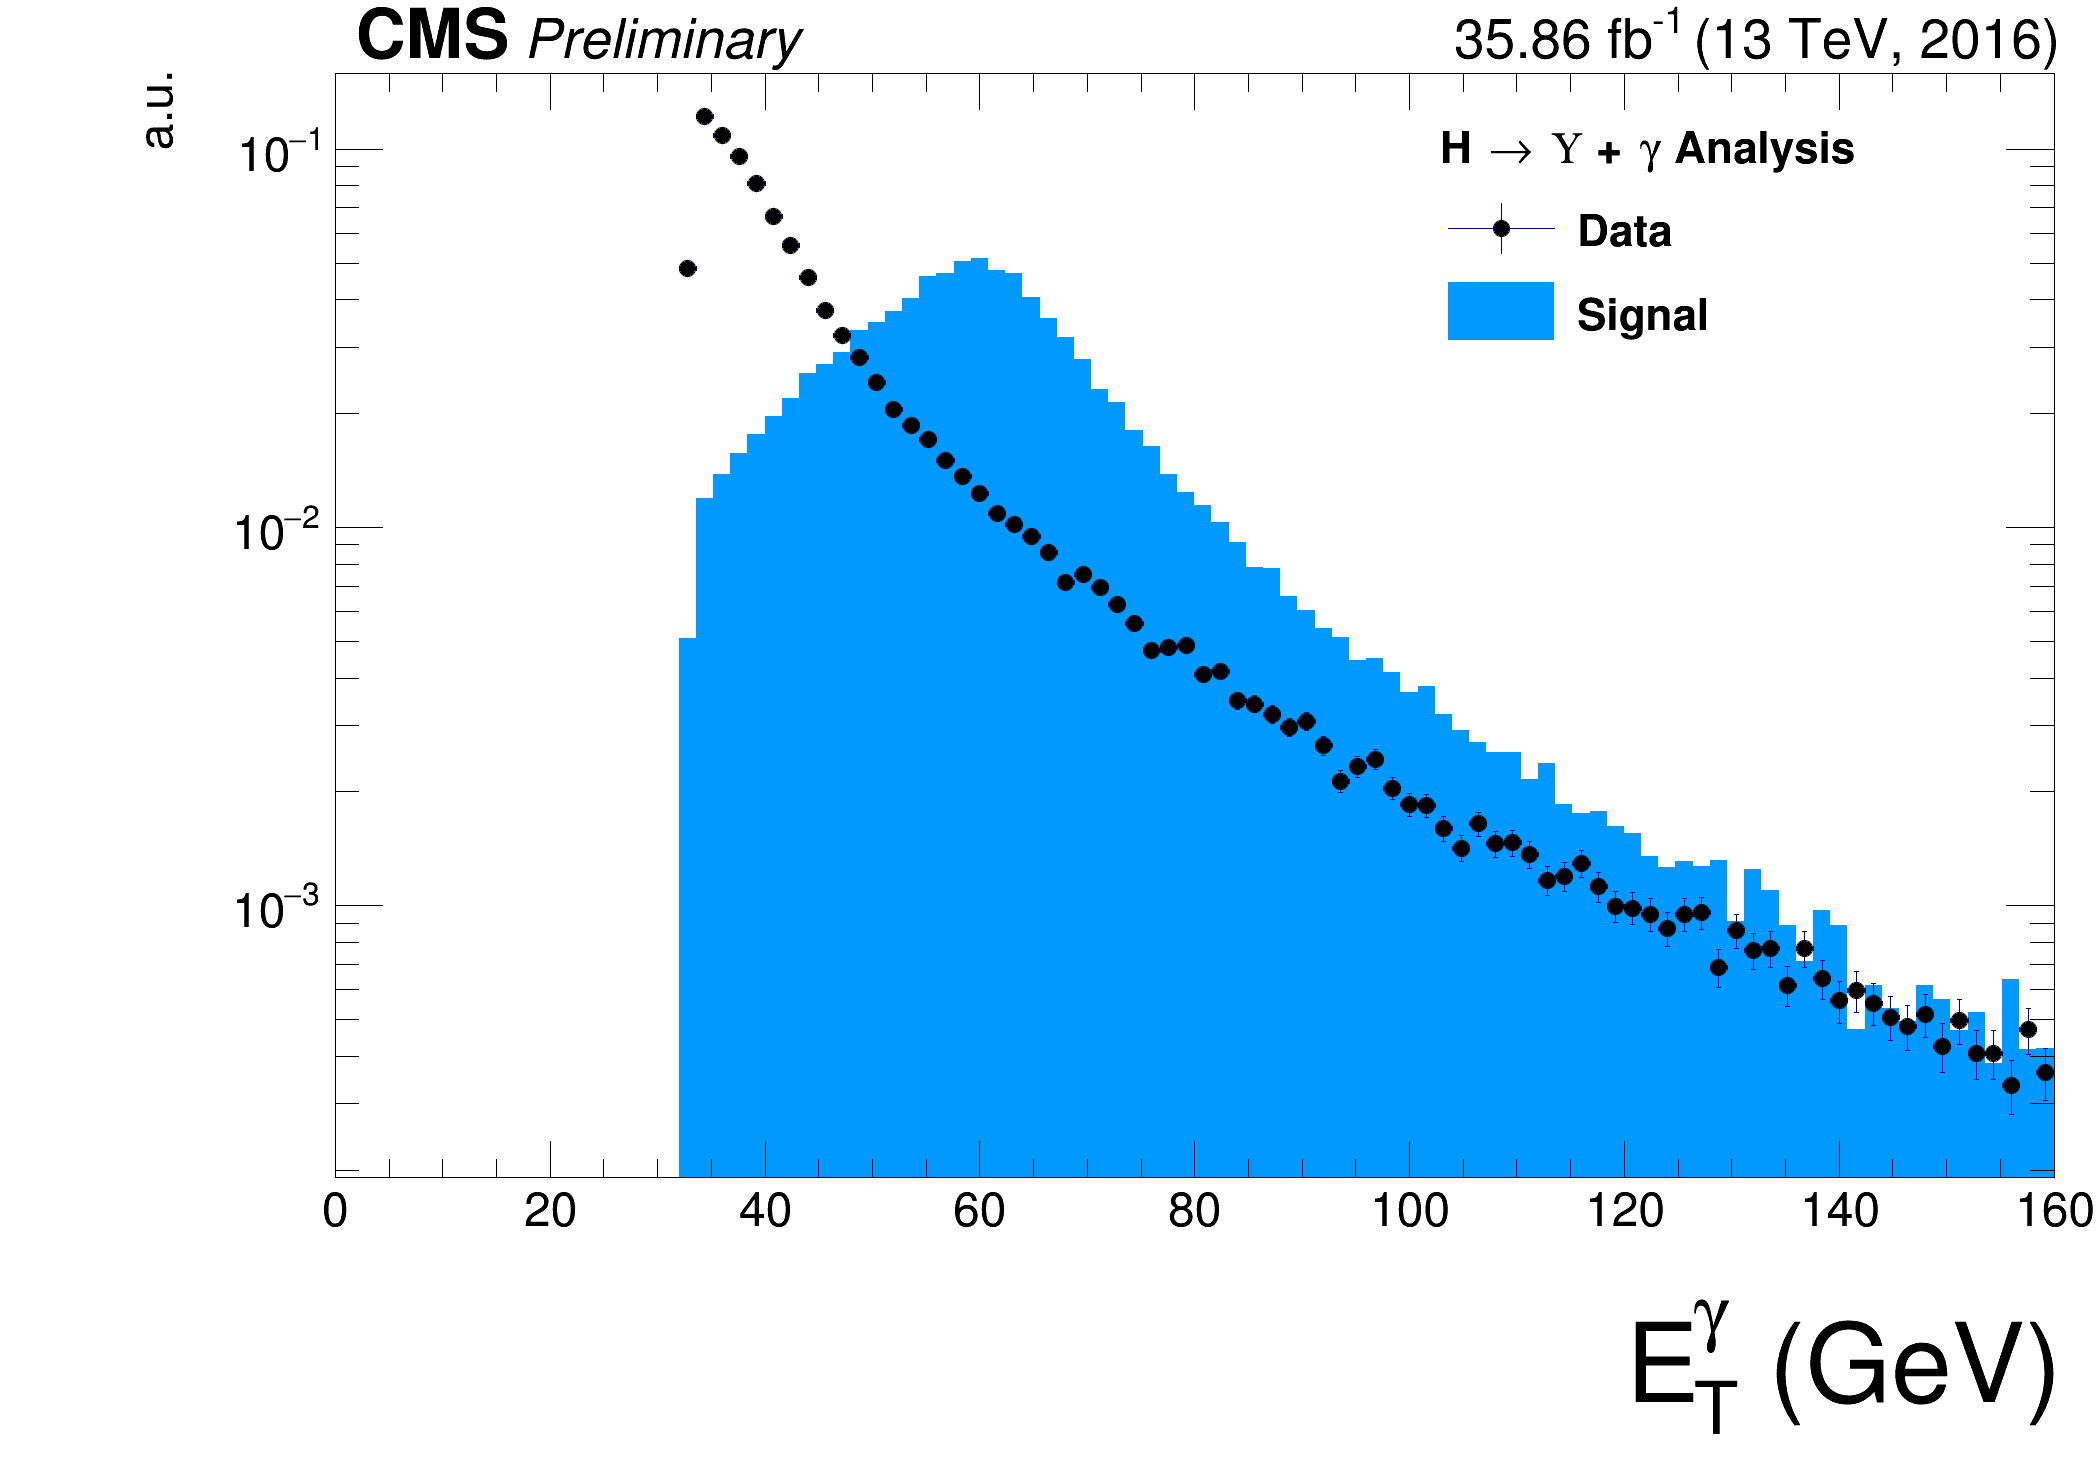
\includegraphics[width=0.45\textwidth]{figures/outputPlots/ZtoUpsilon_Cat0_ZZZZZ/au/data_x_mc/noKinCuts/h_noKin_Photon_pt}\hspace*{1.cm}
\end{center}\vspace*{-.5cm}
\caption{The \PT photon distributions from data and signal events for Z decaying in $\Upsilon(1S,2S,3S)$ + $\gamma$ Group I of selection cuts. The plots normalized to the unit of area.}
\label{fig:pTPhoton_ZtoUpsilon_Cat0}
\end{figure}


%%%%%%%$\eta$ Photon distributions for ZtoUpsilon_Cat0
\begin{figure}[!htbp]
\begin{center}
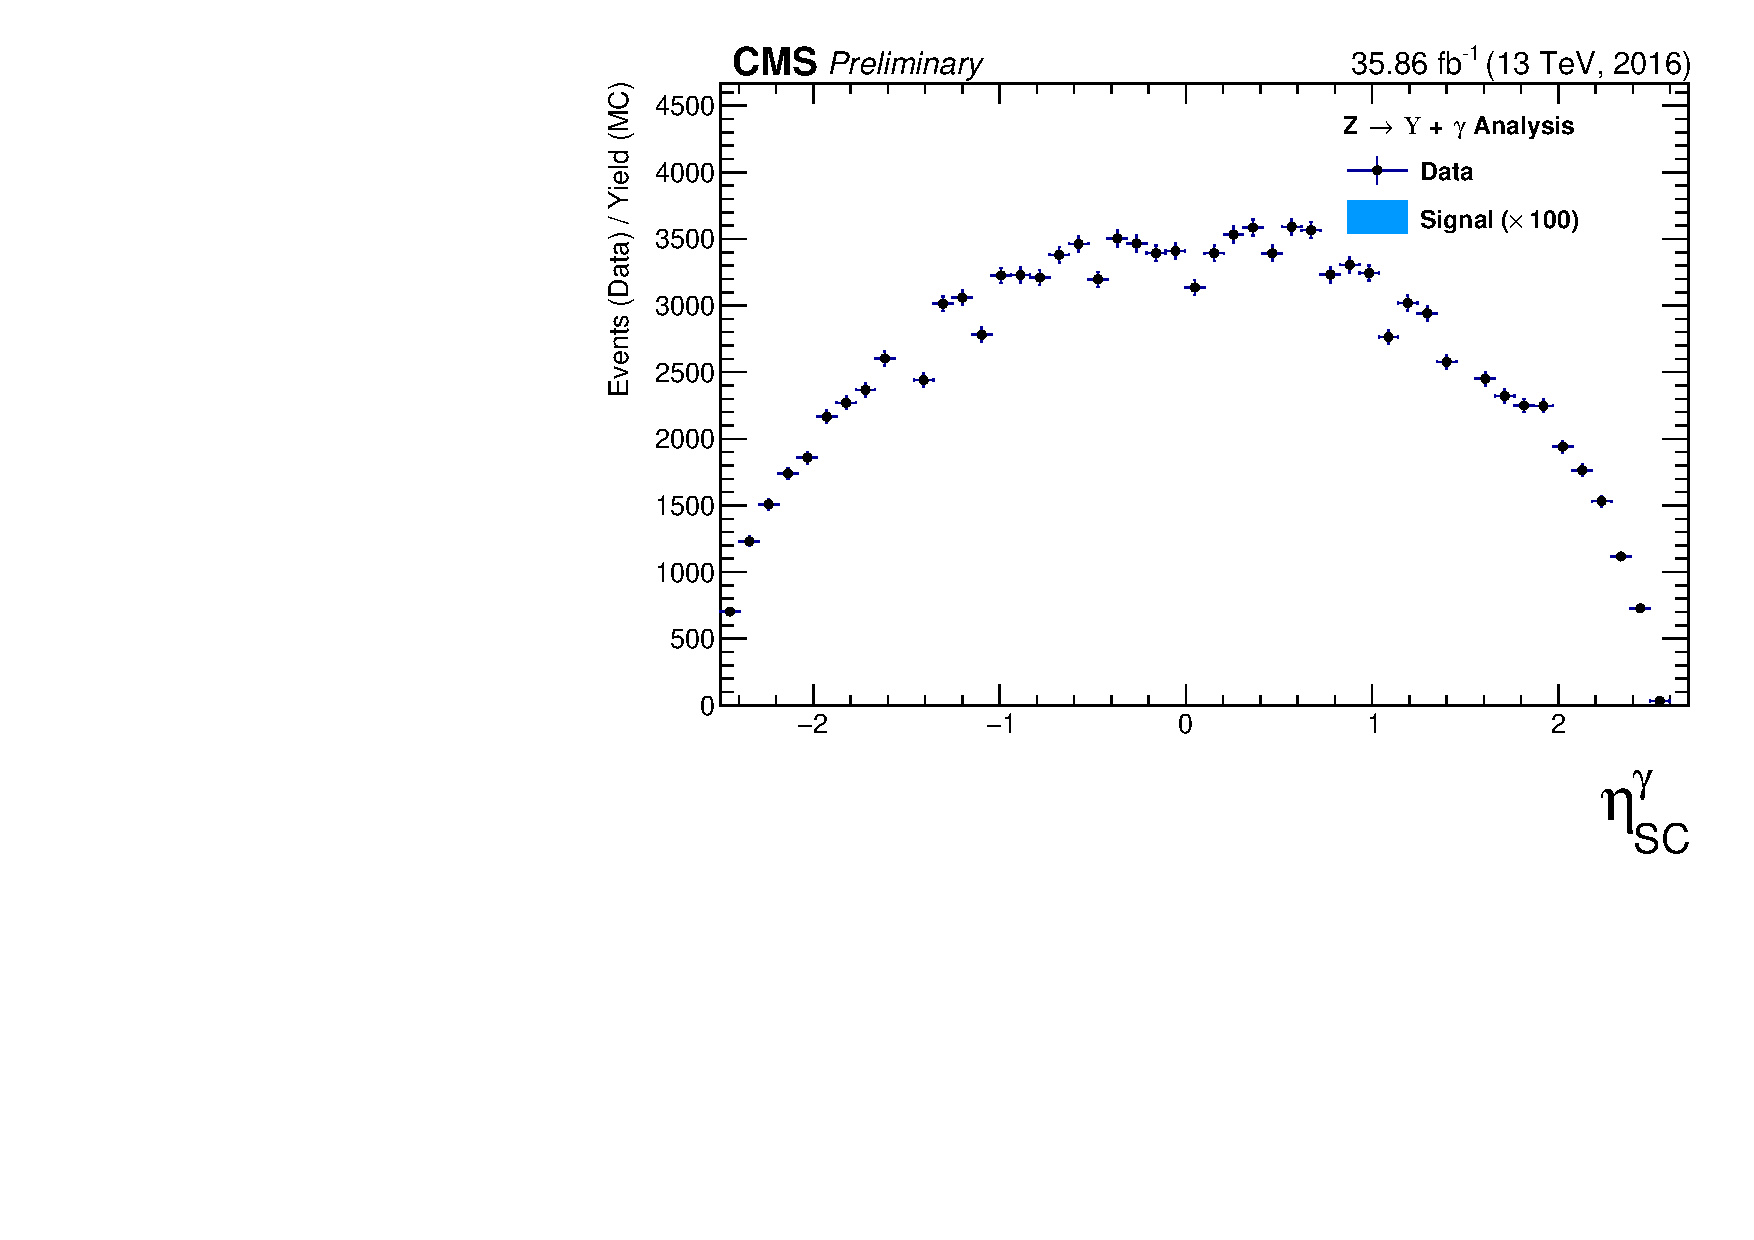
\includegraphics[width=0.45\textwidth]{figures/outputPlots/ZtoUpsilon_Cat0_ZZZZZ/au/data_x_mc/noKinCuts/h_noKin_Photon_eta}\hspace*{1.cm}
\end{center}\vspace*{-.5cm}
\caption{The $\eta$ photon distributions from data and signal events of Z decaying in $\Upsilon(1S,2S,3S)$ + $\gamma$ after Group I of selection cuts. The plot is normalized to the unit of area.}
\label{fig:etaPhoton_ZtoUpsilon_Cat0}
\end{figure}

%%%%%%%%% $\phi$ Photon distributions for ZtoUpsilon_Cat0
\begin{figure}[!htbp]
\begin{center}
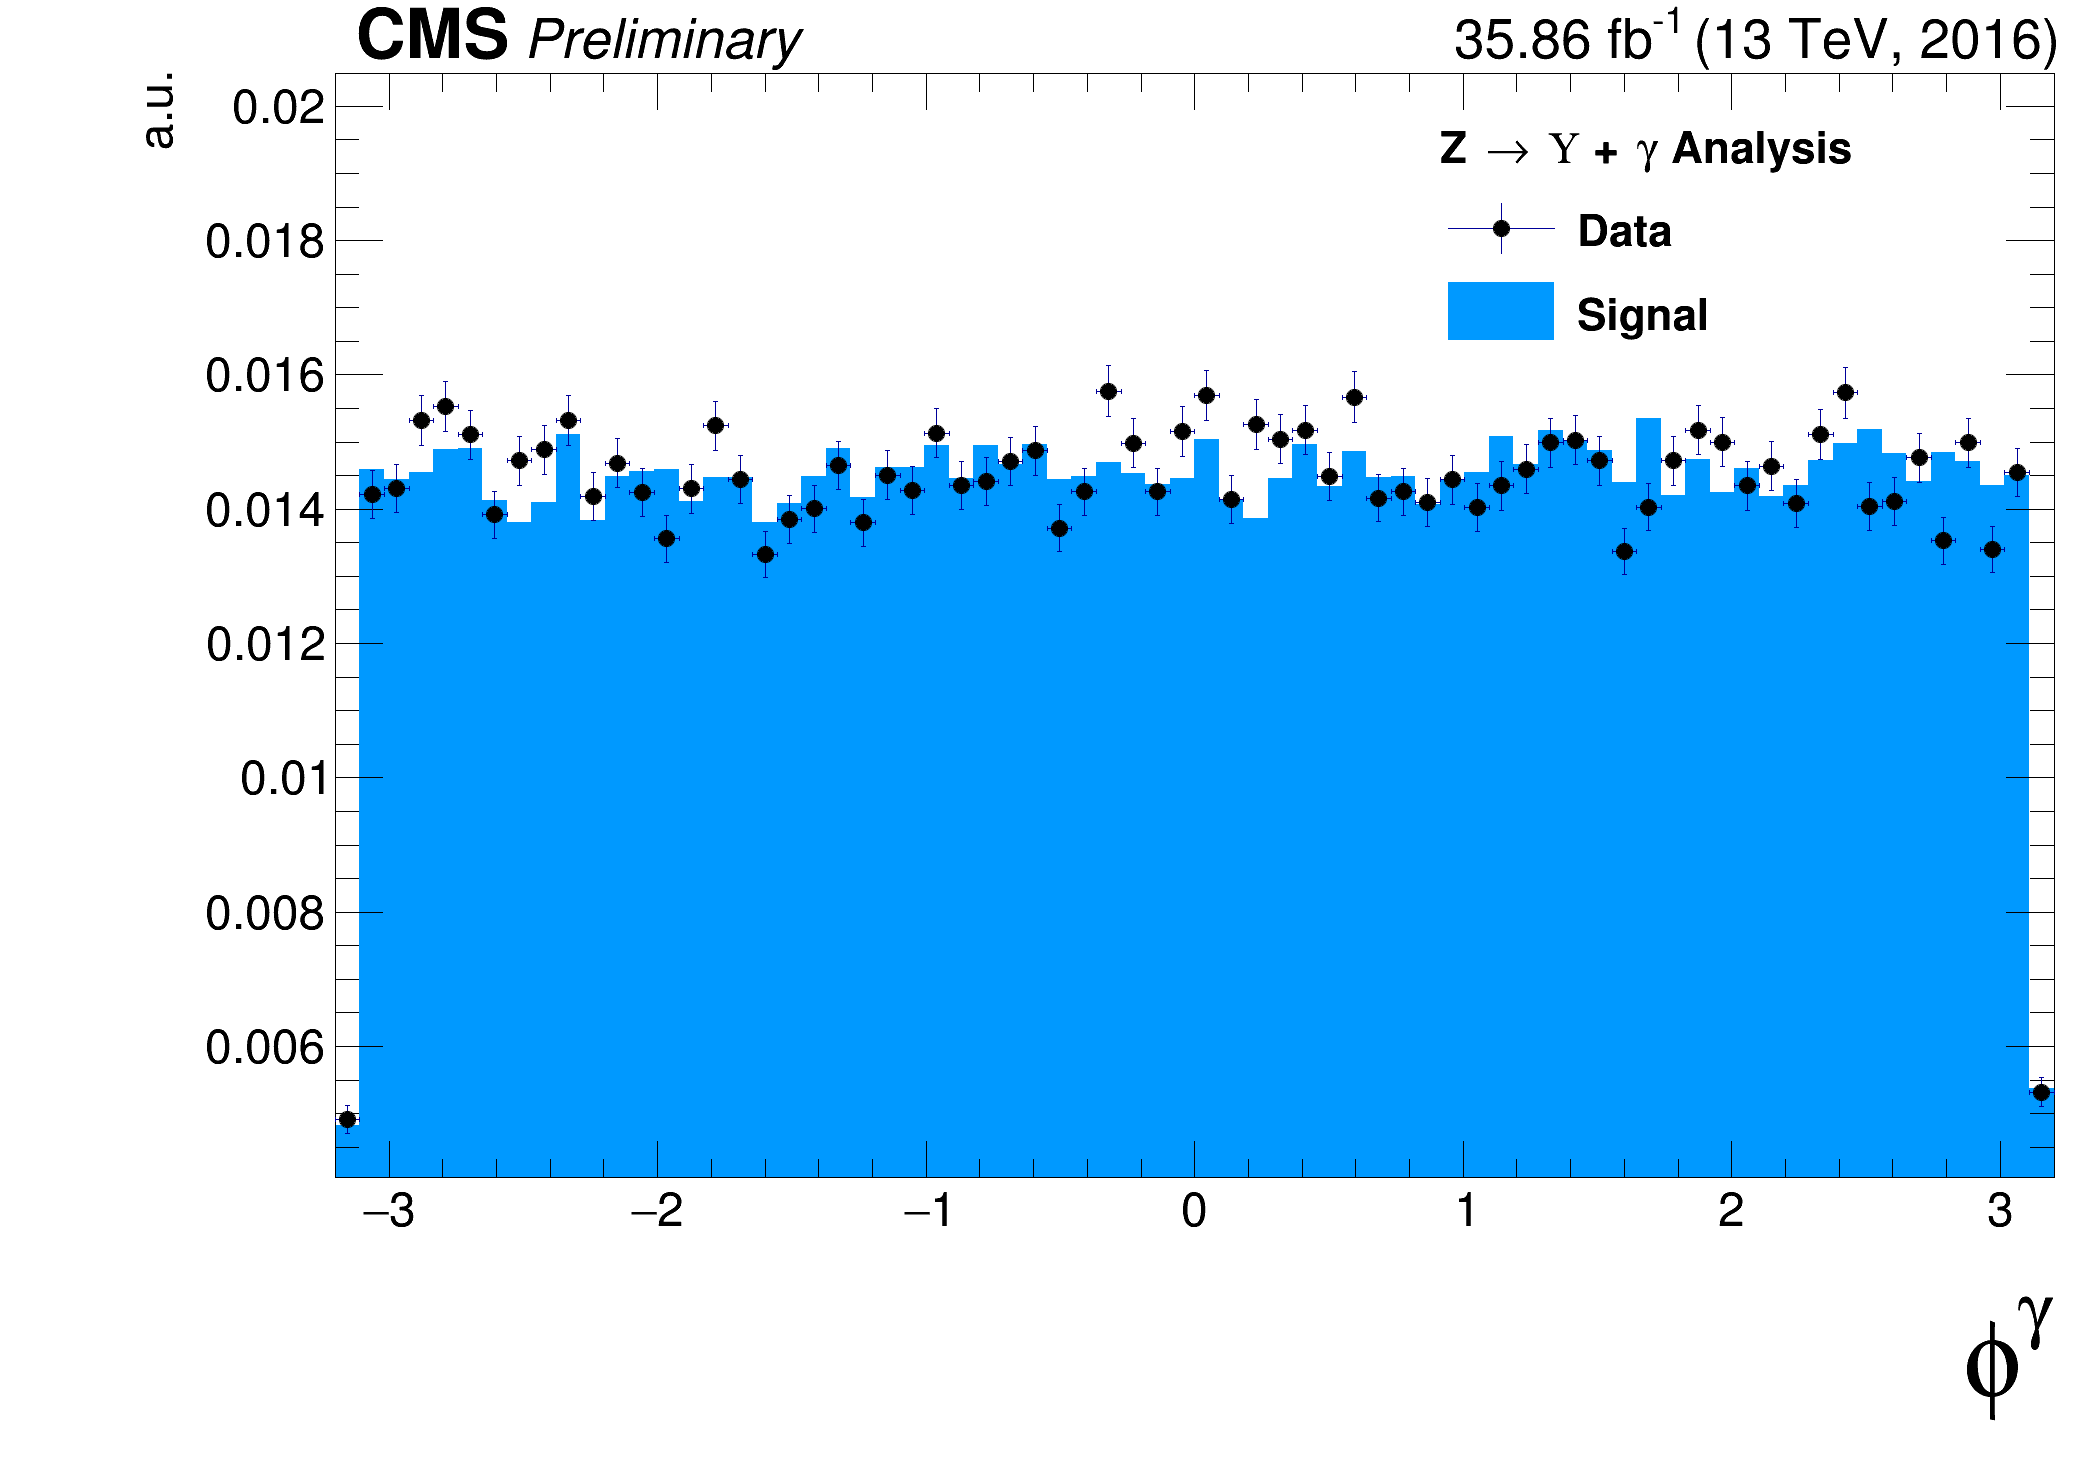
\includegraphics[width=0.45\textwidth]{figures/outputPlots/ZtoUpsilon_Cat0_ZZZZZ/au/data_x_mc/noKinCuts/h_noKin_Photon_phi}\hspace*{1.cm}
\end{center}\vspace*{-.5cm}
\caption{The $\phi$ photon distributions from data and signal events of Z decaying in $\Upsilon(1S,2S,3S)$ + $\gamma$ after Group I of selection cuts. The plot is normalized to the unit of area.}
\label{fig:phiPhoton_ZtoUpsilon_Cat0}
\end{figure}

%%%%%%%%%%%%%
% Upsilon and Z boson
%%$\pT$ Upsilon_and_Higgs distributions for ZtoUpsilon_Cat0
\begin{figure}[!htbp]
\begin{center}
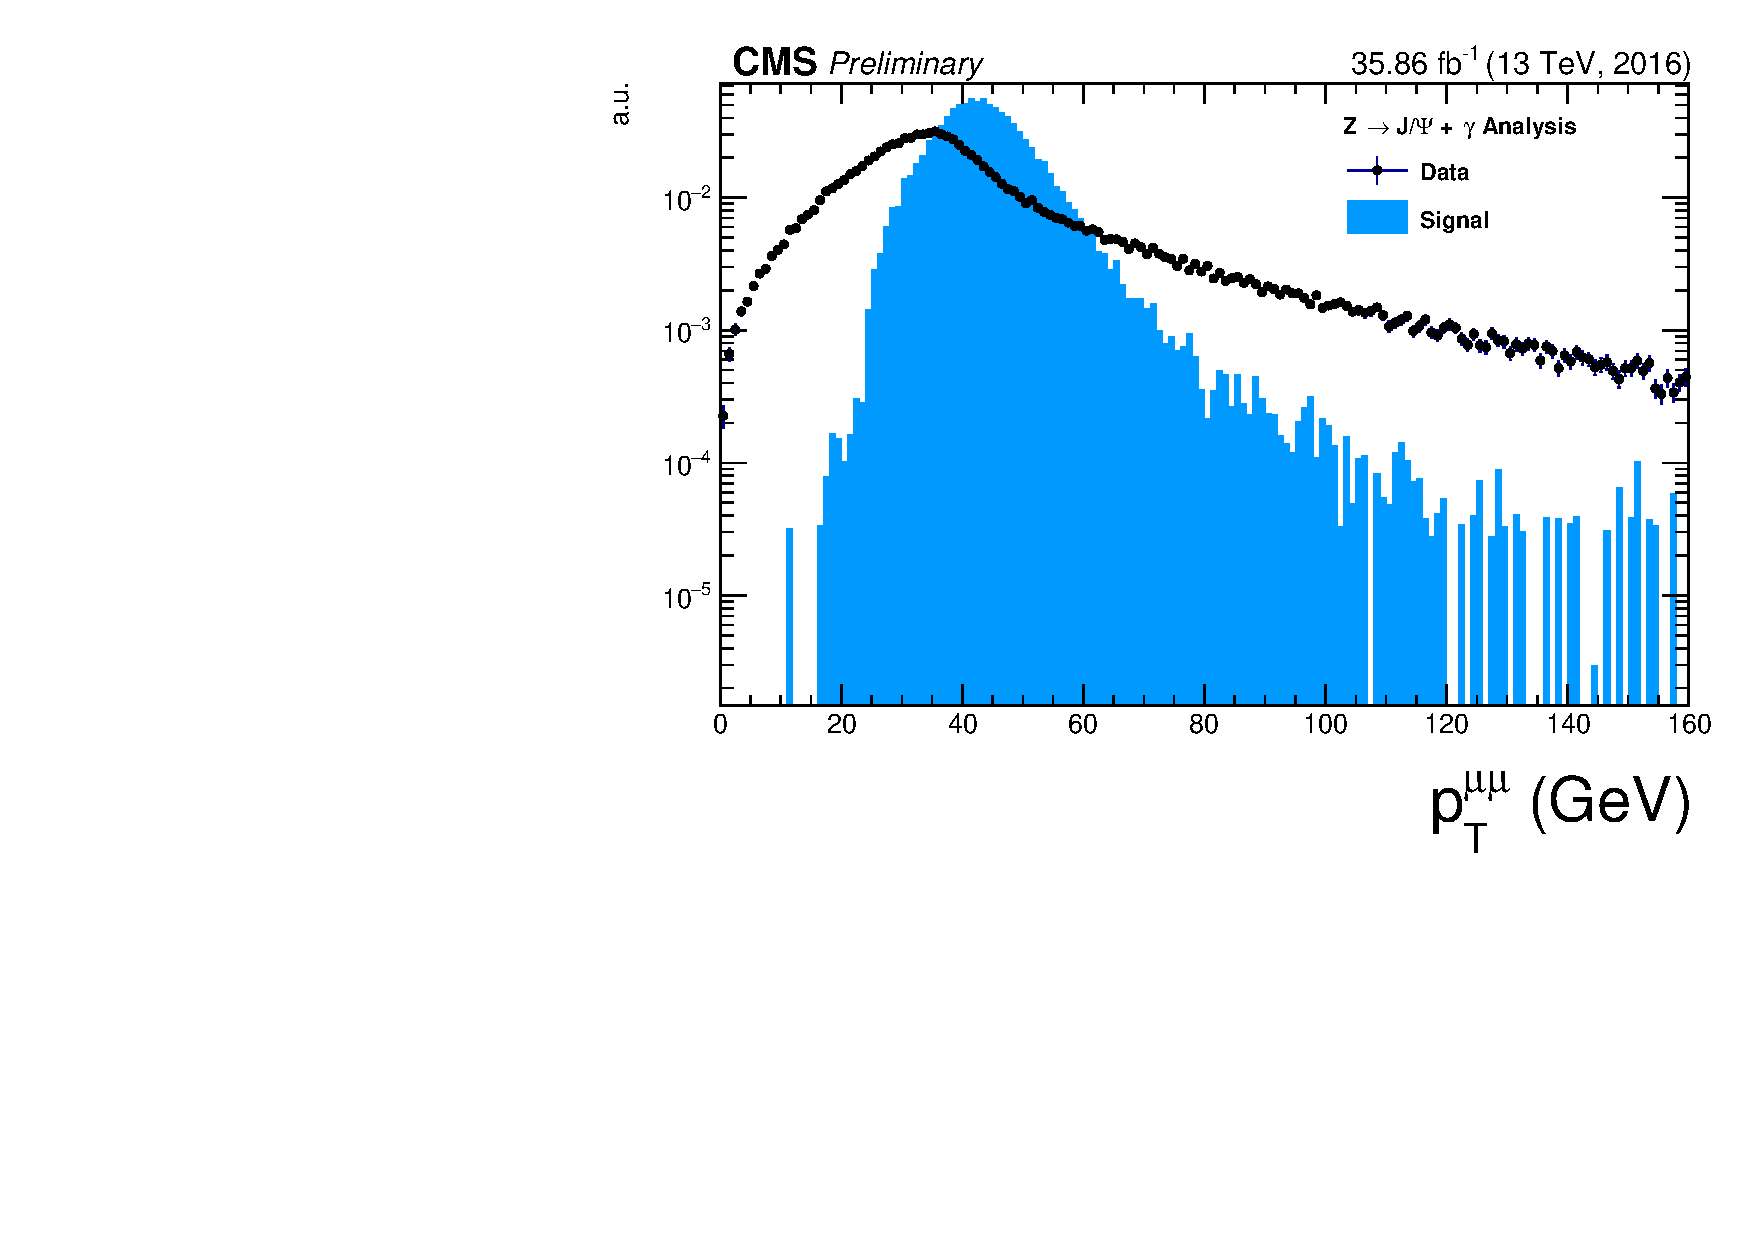
\includegraphics[width=0.45\textwidth]{figures/outputPlots/ZtoUpsilon_Cat0_ZZZZZ/au/data_x_mc/noKinCuts/h_noKin_Upsilon_Pt}\hspace*{1.cm}
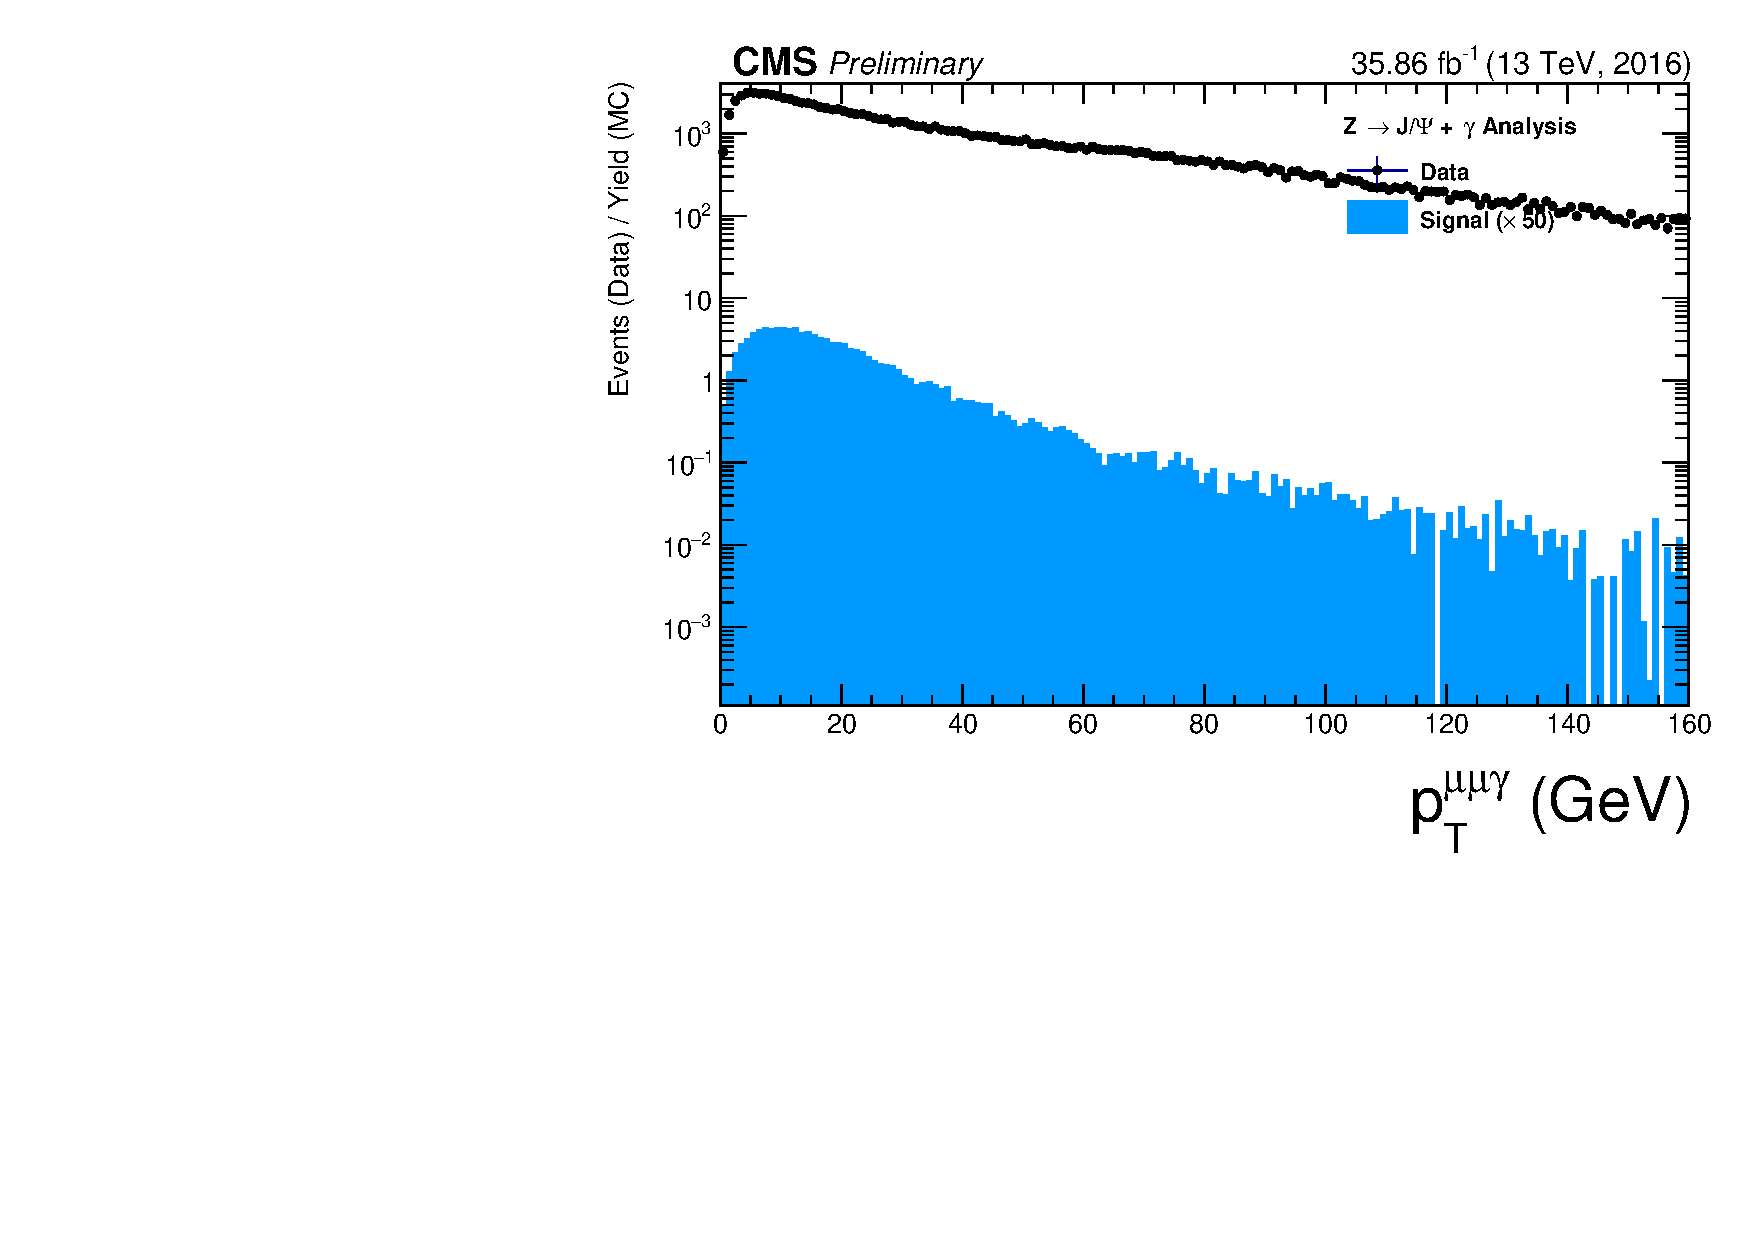
\includegraphics[width=0.45\textwidth]{figures/outputPlots/ZtoUpsilon_Cat0_ZZZZZ/au/data_x_mc/noKinCuts/h_noKin_Z_Pt}
\end{center}\vspace*{-.5cm}
\caption{The \PT distributions for the reconstructed $\Upsilon(1S,2S,3S)$ in the left and for Z in the right from data and signal events for Z decaying in $\Upsilon(1S,2S,3S)$ + $\gamma$ after Group I of selection cuts. The plots are normalized to the unit of area.}
\label{fig:pTUpsilon_and_Z_ZtoUpsilon_Cat0}
\end{figure}


%%%%%%%$\eta$ Upsilon_and_Z distributions for ZtoUpsilon_Cat0
\begin{figure}[!htbp]
\begin{center}
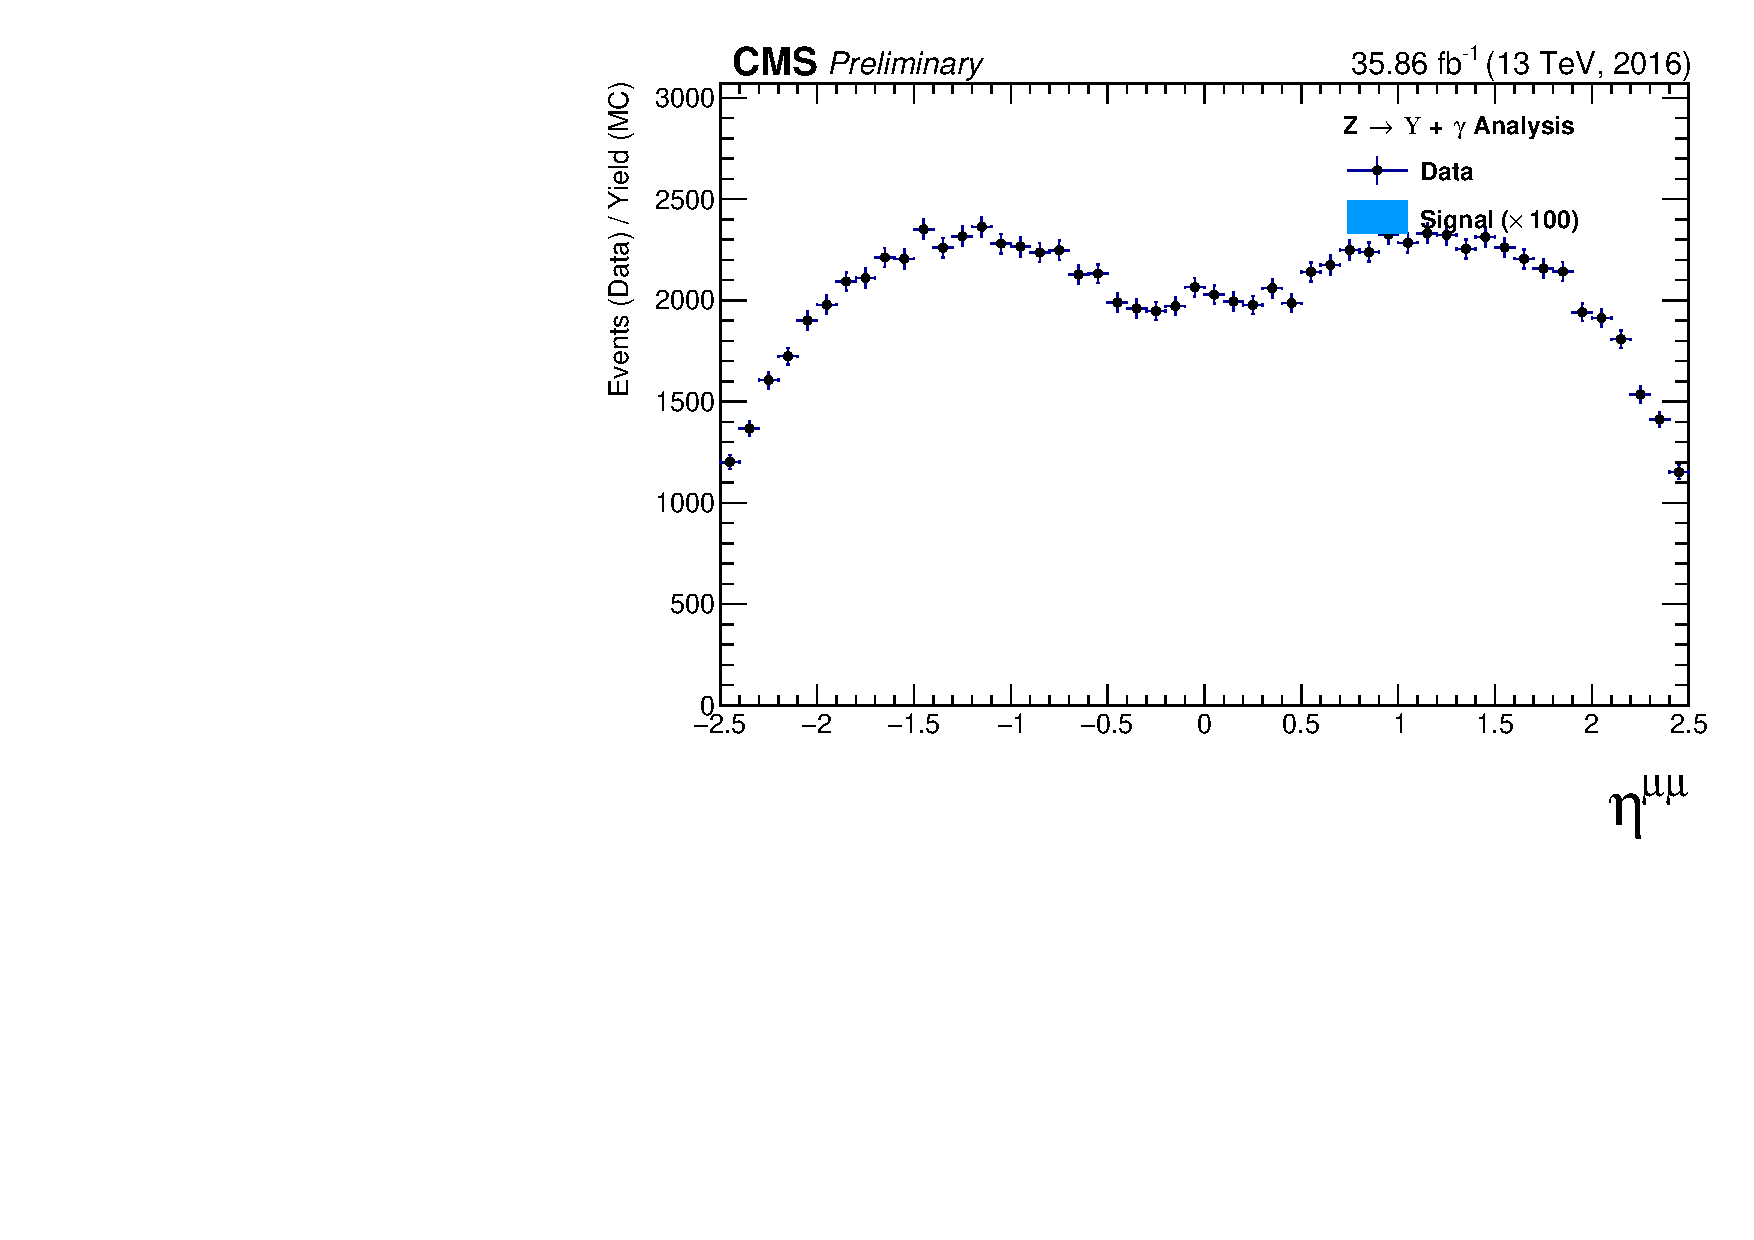
\includegraphics[width=0.45\textwidth]{figures/outputPlots/ZtoUpsilon_Cat0_ZZZZZ/au/data_x_mc/noKinCuts/h_noKin_Upsilon_eta}\hspace*{1.cm}
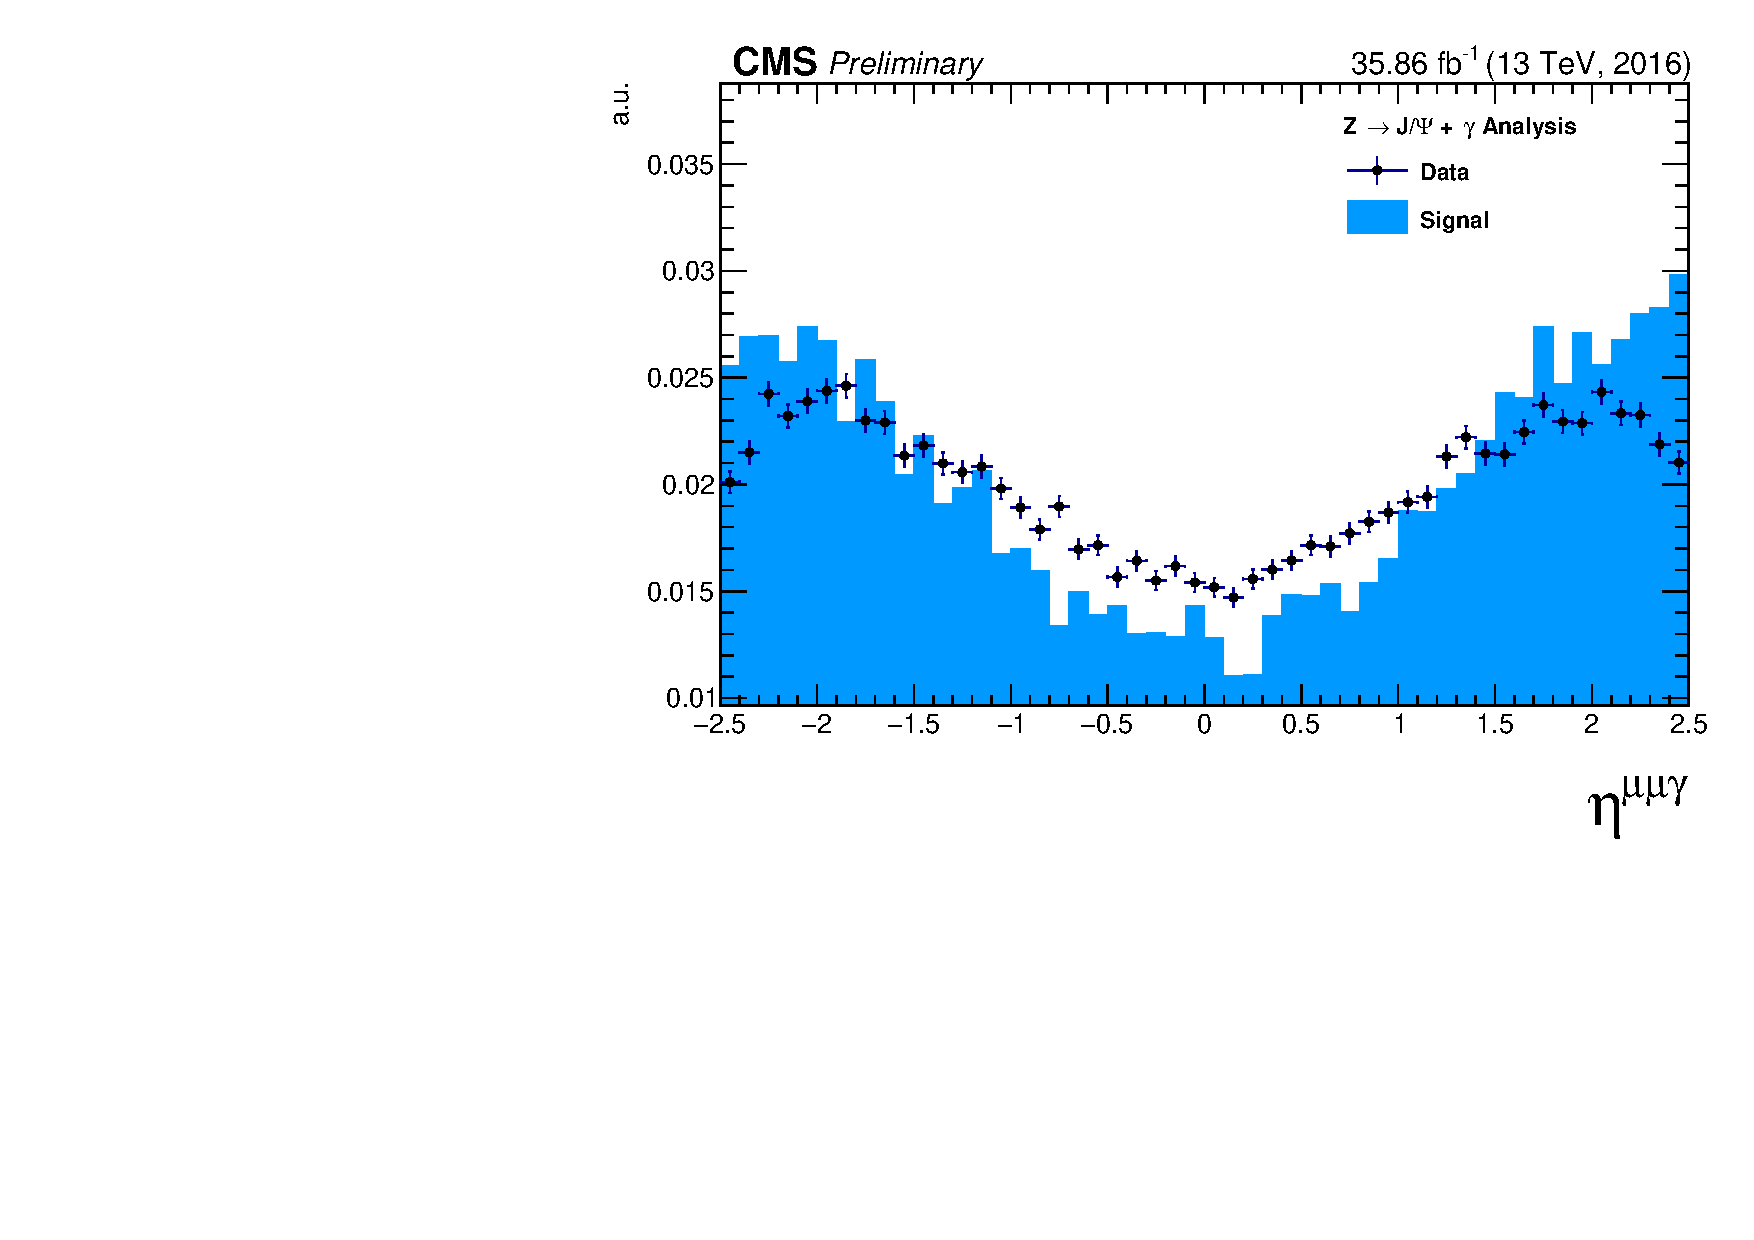
\includegraphics[width=0.45\textwidth]{figures/outputPlots/ZtoUpsilon_Cat0_ZZZZZ/au/data_x_mc/noKinCuts/h_noKin_Z_eta}
\end{center}\vspace*{-.5cm}
\caption{The $\eta$ distributions for $\Upsilon(1S,2S,3S)$ in the left and for Z in the right from data and signal events for Z decaying in $\Upsilon(1S,2S,3S)$ + $\gamma$ after Group I of selection cuts. The plots are normalized to the unit of area.}
\label{fig:etaUpsilon_and_Z_ZtoUpsilon_Cat0}
\end{figure}

%%%%%%%%% $\phi$ Upsilon_and_Zdistributions for ZtoUpsilon_Cat0
\begin{figure}[!htbp]
\begin{center}
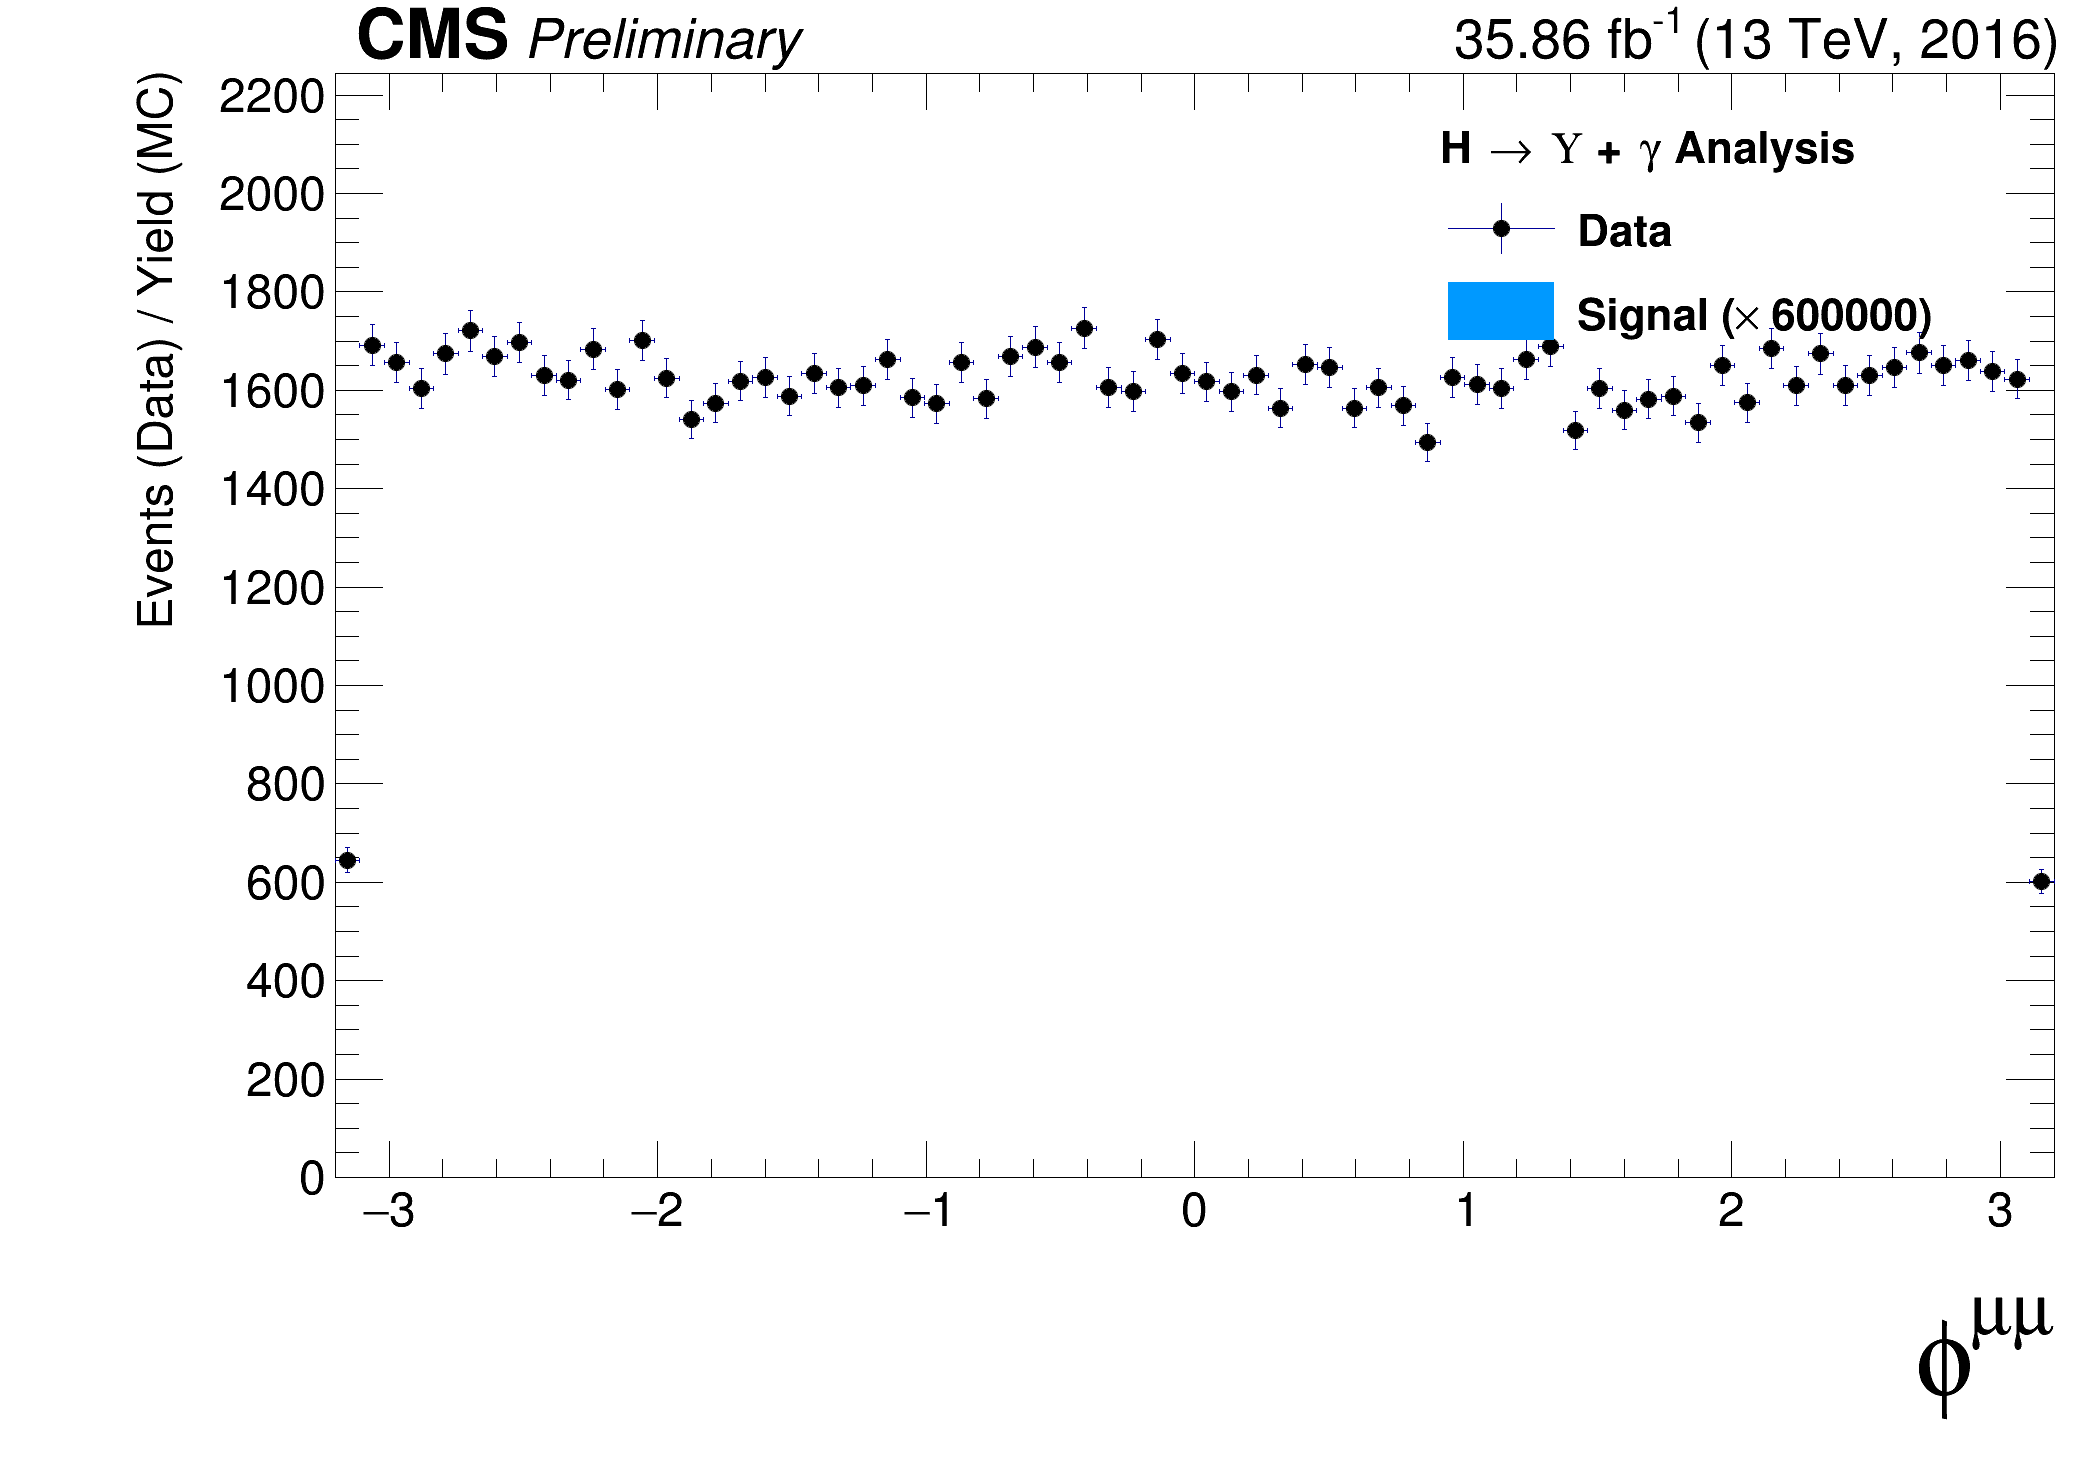
\includegraphics[width=0.45\textwidth]{figures/outputPlots/ZtoUpsilon_Cat0_ZZZZZ/au/data_x_mc/noKinCuts/h_noKin_Upsilon_phi}\hspace*{1.cm}
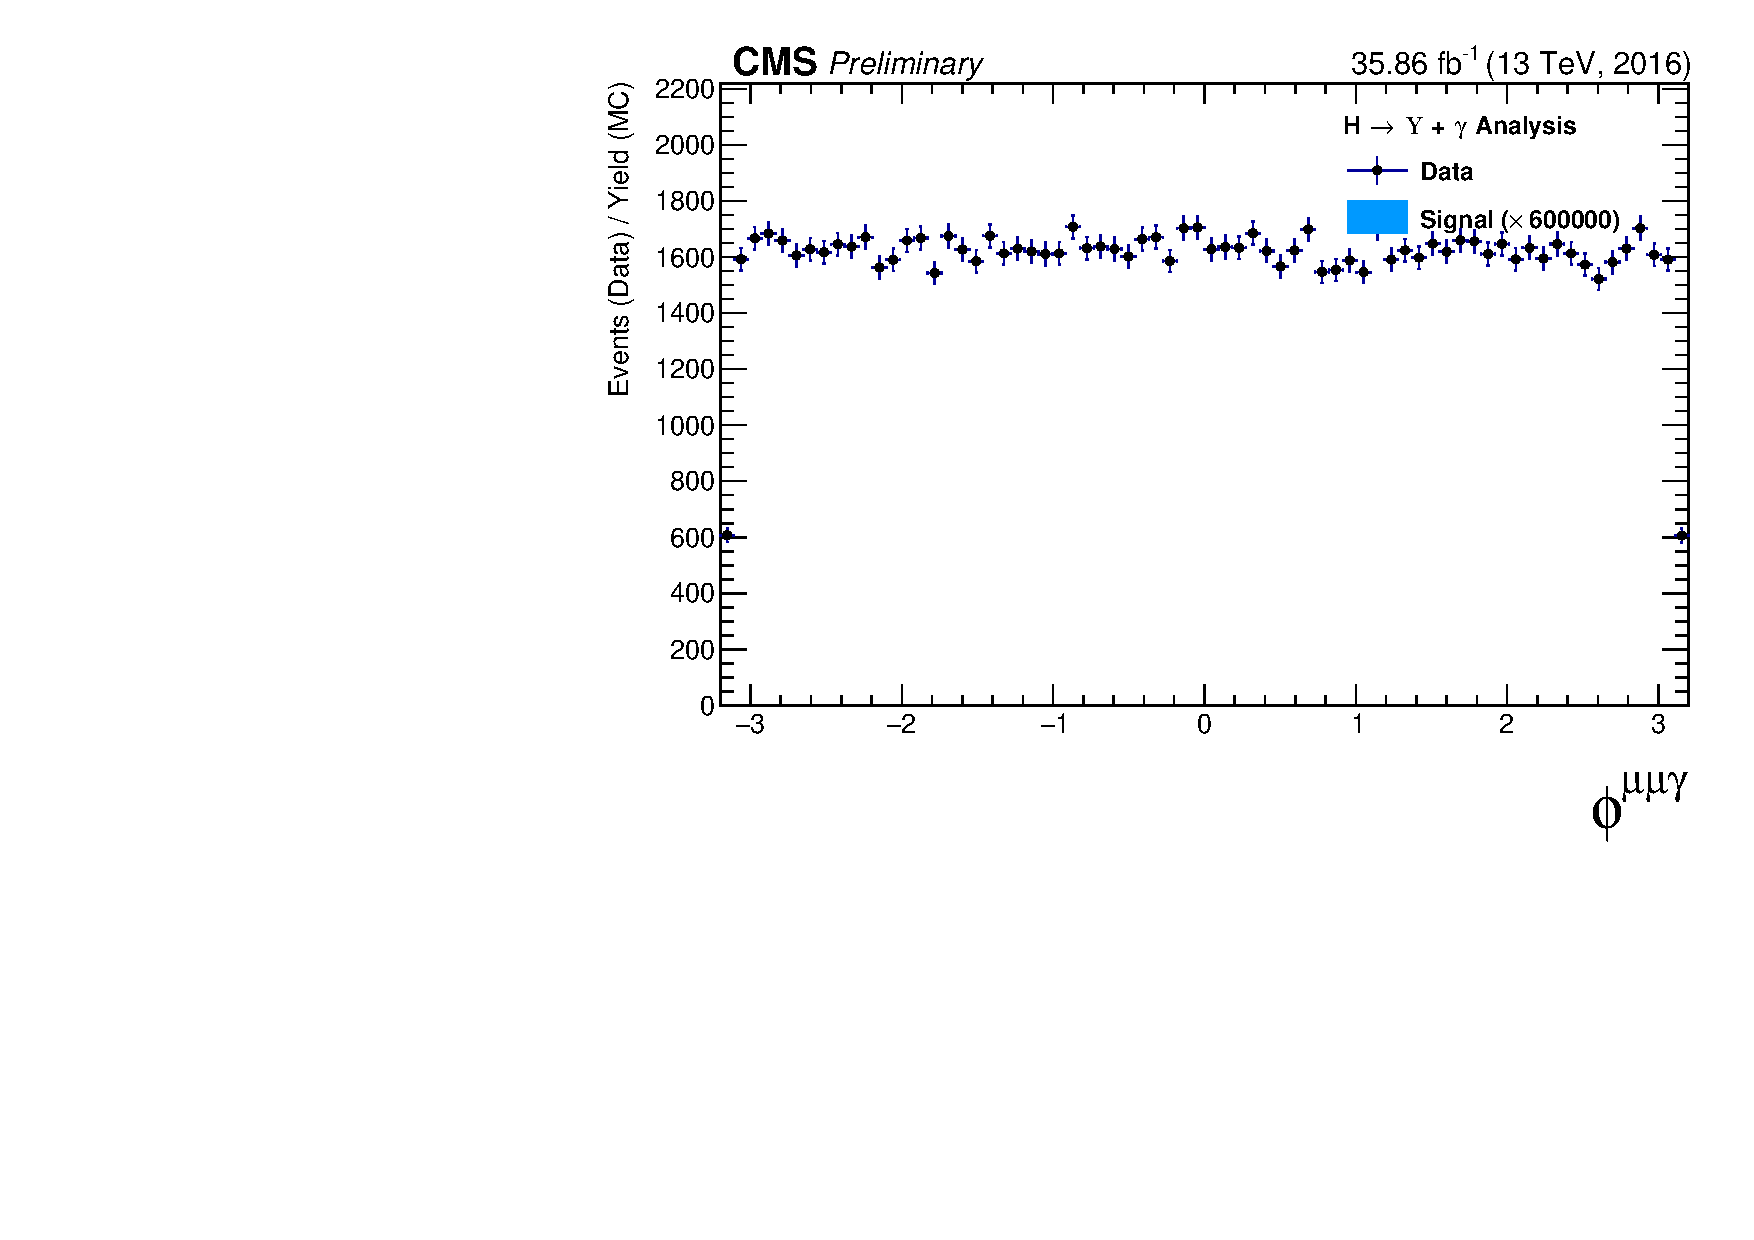
\includegraphics[width=0.45\textwidth]{figures/outputPlots/ZtoUpsilon_Cat0_ZZZZZ/au/data_x_mc/noKinCuts/h_noKin_Z_phi}
\end{center}\vspace*{-.5cm}
\caption{The $\phi$ distributions for $\Upsilon(1S,2S,3S)$ in the left and for Z in the right from data and signal events for Z decaying in $\Upsilon(1S,2S,3S)$ + $\gamma$ after Group I of selection cuts. The plots are normalized to the unit of area.}
\label{fig:phiUpsilon_and_Z_ZtoUpsilon_Cat0}
\end{figure}

%%%%%%%%%%%%

%%%%%%%%%%%%%
% kin cuts
%% delta R -  mu x photon distributions for ZtoUpsilon_Cat0
\begin{figure}[!htbp]
\begin{center}
\includegraphics[width=0.45\textwidth]{figures/outputPlots/ZtoUpsilon_Cat0_ZZZZZ/au/data_x_mc/noKinCuts/h_noKin_deltaR_Leading_Photon}\hspace*{1.cm}
\includegraphics[width=0.45\textwidth]{figures/outputPlots/ZtoUpsilon_Cat0_ZZZZZ/au/data_x_mc/noKinCuts/h_noKin_deltaR_Trailing_Photon}\end{center}\vspace*{-.5cm}
\caption{The $\Delta R$ distributions between the photon and the leading muon (left) and the trailing muon (right) for for Z decaying in $\Upsilon(1S,2S,3S)$ + $\gamma$ from data and signal events after Group I of selection cuts. The plots are normalized to the unit of area.}
\label{fig:deltaR_ZtoUpsilon_Cat0}
\end{figure}

%% delta R and Delta Phi -  MuMu x photon distributions for ZtoUpsilon_Cat0
\begin{figure}[!htbp]
\begin{center}
\includegraphics[width=0.45\textwidth]{figures/outputPlots/ZtoUpsilon_Cat0_ZZZZZ/au/data_x_mc/noKinCuts/h_noKin_deltaR_Upsilon_Photon}\hspace*{1.cm}
\includegraphics[width=0.45\textwidth]{figures/outputPlots/ZtoUpsilon_Cat0_ZZZZZ/au/data_x_mc/noKinCuts/h_noKin_deltaPhi_Upsilon_Photon}\end{center}\vspace*{-.5cm}
\caption{Left: The $\Delta R$ distributions between reconstructed dimuon ($\mu\mu$) system and the photon. Right: absolute value of the $\Delta \phi$ between the leading muon and the photon for for Z decaying in $\Upsilon(1S,2S,3S)$ + $\gamma$ from data and signal events after Group I of selection cuts. The plots are normalized to the unit of area.}
\label{fig:deltaRdeltaPhi_ZtoUpsilon_Cat0}
\end{figure}


%%%%%%% energy/mass ratio distributions for ZtoUpsilon_Cat0
\begin{figure}[!htbp]
\begin{center}
\includegraphics[width=0.45\textwidth]{figures/outputPlots/ZtoUpsilon_Cat0_ZZZZZ/au/data_x_mc/noKinCuts/h_noKin_upsilonPt_over_zMass}\hspace*{1.cm}
\includegraphics[width=0.45\textwidth]{figures/outputPlots/ZtoUpsilon_Cat0_ZZZZZ/au/data_x_mc/noKinCuts/h_noKin_photonPt_over_zMass}
\end{center}\vspace*{-.5cm}
\caption{The ratio for the transverse momentum of the reconstructed Upsilon and the reconstructed Z mass ($p_{T}^{\mu\mu}/M_{\mu\mu\gamma}$ - left) and the ratio for the transverse energy of the reconstructed Photon and the reconstructed Z mass ($E_{T}^{\mu\mu}/M_{\mu\mu\gamma}$ - right) distribution for Z decaying in $\Upsilon(1S,2S,3S)$ + $\gamma$ from data and signal events after Group I of selection cuts. The plots are normalized to the unit of area.}
\label{fig:energy_ration_ZtoUpsilon_Cat0}
\end{figure}

%%%%%%%%% dimuon mass distributions for ZtoUpsilon_Cat0
\begin{figure}[!htbp]
\begin{center}
\includegraphics[width=0.45\textwidth]{figures/outputPlots/ZtoUpsilon_Cat0_ZZZZZ/nEvts/data_x_mc/noKinCuts/h_noKin_Upsilon_Mass_Signal_and_Background_LargeRange}\hspace*{1.cm}
\end{center}\vspace*{-.5cm}
\caption{The dimuon mass distribution of the reconstructed $\Upsilon (1S,2S,3S)$ from data and signal events for Z decaying after Group I of selection cuts. The plot is normalized to the number of events. "Signal" stands for the $Z \rightarrow \Upsilon (1S,2S,3S) + \gamma$ sample (scaled by a factor of $\times 100$) and "Background" corresponds to the peaking background ($Z \rightarrow \mu\mu\gamma_{FSR}$) sample (scaled by a factor of x3).}
\label{fig:dimuon_mass_ZtoUpsilon_Cat0}
\end{figure}

%%%%%%%%%%%%


%CONTROL PLOTS
%%$\pT$ muon distributions for HtoUpsilon_Cat0
\begin{figure}[!htbp]
\begin{center}
\includegraphics[width=0.45\textwidth]{figures/outputPlots/HtoUpsilon_Cat0_ZZZZZ/au/data_x_mc/noKinCuts/h_noKin_TrailingMu_pt}\hspace*{1.cm}
\includegraphics[width=0.45\textwidth]{figures/outputPlots/HtoUpsilon_Cat0_ZZZZZ/au/data_x_mc/noKinCuts/h_noKin_LeadingMu_pt}
\end{center}\vspace*{-.5cm}
\caption{The \PT muon distributions from data and signal events for Higgs decaying in $\Upsilon(1S,2S,3S)$ + $\gamma$ after Group I of selection cuts, where on left are presenting the trailing muons and on right are the leading muons. The plots are normalized to the unit of area.}
\label{fig:pTMuons_HtoUpsilon_Cat0}
\end{figure}


%%%%%%%$\eta$ muon distributions for HtoUpsilon_Cat0
\begin{figure}[!htbp]
\begin{center}
\includegraphics[width=0.45\textwidth]{figures/outputPlots/HtoUpsilon_Cat0_ZZZZZ/au/data_x_mc/noKinCuts/h_noKin_TrailingMu_eta}\hspace*{1.cm}
\includegraphics[width=0.45\textwidth]{figures/outputPlots/HtoUpsilon_Cat0_ZZZZZ/au/data_x_mc/noKinCuts/h_noKin_LeadingMu_eta}
\end{center}\vspace*{-.5cm}
\caption{The $\eta$ muon distributions from data and signal events of Higgs decaying in $\Upsilon(1S,2S,3S)$ + $\gamma$ after Group I of selection cuts, where on left are presenting the trailing muons and on right are the leading muons. The plots are normalized to the unit of area.}
\label{fig:etaMuons_HtoUpsilon_Cat0}
\end{figure}

%%%%%%%%% $\phi$ muon distributions for HtoUpsilon_Cat0
\begin{figure}[!htbp]
\begin{center}
\includegraphics[width=0.45\textwidth]{figures/outputPlots/HtoUpsilon_Cat0_ZZZZZ/au/data_x_mc/noKinCuts/h_noKin_TrailingMu_phi}\hspace*{1.cm}
\includegraphics[width=0.45\textwidth]{figures/outputPlots/HtoUpsilon_Cat0_ZZZZZ/au/data_x_mc/noKinCuts/h_noKin_LeadingMu_phi}
\end{center}\vspace*{-.5cm}
\caption{The $\phi$ muon distributions from data and signal events of Higgs decaying in $\Upsilon(1S,2S,3S)$ + $\gamma$ after Group I of selection cuts, where on left are presenting the trailing muons and on right are the leading muons. The plots are normalized to the unit of area.}
\label{fig:phiMuons_HtoUpsilon_Cat0}
\end{figure}

%%%%%%%%%%%%%

%photon
%%$\pT$ Photon distributions for HtoUpsilon_Cat0
\begin{figure}[!htbp]
\begin{center}
\includegraphics[width=0.45\textwidth]{figures/outputPlots/HtoUpsilon_Cat0_ZZZZZ/au/data_x_mc/noKinCuts/h_noKin_Photon_pt}\hspace*{1.cm}
\end{center}\vspace*{-.5cm}
\caption{The \PT photon distributions from data and signal events for Higgs decaying in $\Upsilon(1S,2S,3S)$ + $\gamma$ Group I of selection cuts. The plot is normalized to the unit of area.}
\label{fig:pTPhoton_HtoUpsilon_Cat0}
\end{figure}


%%%%%%%$\eta$ Photon distributions for HtoUpsilon_Cat0
\begin{figure}[!htbp]
\begin{center}
\includegraphics[width=0.45\textwidth]{figures/outputPlots/HtoUpsilon_Cat0_ZZZZZ/au/data_x_mc/noKinCuts/h_noKin_Photon_eta}\hspace*{1.cm}
\end{center}\vspace*{-.5cm}
\caption{The $\eta$ photon distributions from data and signal events of Higgs decaying in $\Upsilon(1S,2S,3S)$ + $\gamma$ after Group I of selection cuts. The plot is normalized to the unit of area.}
\label{fig:etaPhoton_HtoUpsilon_Cat0}
\end{figure}

%%%%%%%%% $\phi$ Photon distributions for HtoUpsilon_Cat0
\begin{figure}[!htbp]
\begin{center}
\includegraphics[width=0.45\textwidth]{figures/outputPlots/HtoUpsilon_Cat0_ZZZZZ/au/data_x_mc/noKinCuts/h_noKin_Photon_phi}\hspace*{1.cm}
\end{center}\vspace*{-.5cm}
\caption{The $\phi$ photon distributions from data and signal events of Higgs decaying in $\Upsilon(1S,2S,3S)$ + $\gamma$ after Group I of selection cuts. The plot is normalized to the unit of area.}
\label{fig:phiPhoton_HtoUpsilon_Cat0}
\end{figure}

%%%%%%%%%%%%%
% Upsilon and Higgs boson
%%$\pT$ Upsilon_and_Higgs distributions for HtoUpsilon_Cat0
\begin{figure}[!htbp]
\begin{center}
\includegraphics[width=0.45\textwidth]{figures/outputPlots/HtoUpsilon_Cat0_ZZZZZ/au/data_x_mc/noKinCuts/h_noKin_Upsilon_Pt}\hspace*{1.cm}
\includegraphics[width=0.45\textwidth]{figures/outputPlots/HtoUpsilon_Cat0_ZZZZZ/au/data_x_mc/noKinCuts/h_noKin_Z_Pt}
\end{center}\vspace*{-.5cm}
\caption{The \PT distributions for $\Upsilon(1S,2S,3S)$ in the left and for Higgs in the right from data and signal events for Higgs decaying in $\Upsilon(1S,2S,3S)$ + $\gamma$ after Group I of selection cuts. The plots are normalized to the unit of area.}
\label{fig:pTUpsilon_and_Higgs_HtoUpsilon_Cat0}
\end{figure}


%%%%%%%$\eta$ Upsilon_and_Higgs distributions for HtoUpsilon_Cat0
\begin{figure}[!htbp]
\begin{center}
\includegraphics[width=0.45\textwidth]{figures/outputPlots/HtoUpsilon_Cat0_ZZZZZ/au/data_x_mc/noKinCuts/h_noKin_Upsilon_eta}\hspace*{1.cm}
\includegraphics[width=0.45\textwidth]{figures/outputPlots/HtoUpsilon_Cat0_ZZZZZ/au/data_x_mc/noKinCuts/h_noKin_Z_eta}
\end{center}\vspace*{-.5cm}
\caption{The $\eta$ distributions for $\Upsilon(1S,2S,3S)$ in the left and for Higgs in the right from data and signal events for Higgs decaying in $\Upsilon(1S,2S,3S)$ + $\gamma$ after Group I of selection cuts. The plots are normalized to the unit of area.}
\label{fig:etaUpsilon_and_Higgs_HtoUpsilon_Cat0}
\end{figure}

%%%%%%%%% $\phi$ Upsilon_and_Higgsdistributions for HtoUpsilon_Cat0
\begin{figure}[!htbp]
\begin{center}
\includegraphics[width=0.45\textwidth]{figures/outputPlots/HtoUpsilon_Cat0_ZZZZZ/au/data_x_mc/noKinCuts/h_noKin_Upsilon_phi}\hspace*{1.cm}
\includegraphics[width=0.45\textwidth]{figures/outputPlots/HtoUpsilon_Cat0_ZZZZZ/au/data_x_mc/noKinCuts/h_noKin_Z_phi}
\end{center}\vspace*{-.5cm}
\caption{The $\phi$ distributions for $\Upsilon(1S,2S,3S)$ in the left and for Higgs in the right from data and signal events for Higgs decaying in $\Upsilon(1S,2S,3S)$ + $\gamma$ after Group I of selection cuts. The plots are normalized to the unit of area.}
\label{fig:phiUpsilon_and_Higgs_HtoUpsilon_Cat0}
\end{figure}

%%%%%%%%%%%%

%%%%%%%%%%%%%
% kin cuts
%% delta R -  mu x photon distributions for HtoUpsilon_Cat0
\begin{figure}[!htbp]
\begin{center}
\includegraphics[width=0.45\textwidth]{figures/outputPlots/HtoUpsilon_Cat0_ZZZZZ/au/data_x_mc/noKinCuts/h_noKin_deltaR_Leading_Photon}\hspace*{1.cm}
\includegraphics[width=0.45\textwidth]{figures/outputPlots/HtoUpsilon_Cat0_ZZZZZ/au/data_x_mc/noKinCuts/h_noKin_deltaR_Trailing_Photon}\end{center}\vspace*{-.5cm}
\caption{The $\Delta R$ distributions between the photon and the leading muon (left) and the trailing muon (right) for Higgs decaying in $\Upsilon(1S,2S,3S)$ + $\gamma$ from data and signal events after Group I of selection cuts. The plots are normalized to the unit of area.}
\label{fig:deltaR_HtoUpsilon_Cat0}
\end{figure}

%% delta R and Delta Phi -  MuMu x photon distributions for HtoUpsilon_Cat0
\begin{figure}[!htbp]
\begin{center}
\includegraphics[width=0.45\textwidth]{figures/outputPlots/HtoUpsilon_Cat0_ZZZZZ/au/data_x_mc/noKinCuts/h_noKin_deltaR_Upsilon_Photon}\hspace*{1.cm}
\includegraphics[width=0.45\textwidth]{figures/outputPlots/HtoUpsilon_Cat0_ZZZZZ/au/data_x_mc/noKinCuts/h_noKin_deltaPhi_Upsilon_Photon}\end{center}\vspace*{-.5cm}
\caption{Left: The $\Delta R$ distributions between reconstructed dimuon ($\mu\mu$) system and the photon. Right: absolute value of the $\Delta \phi$ between the leading muon and the photon for for Higgs decaying in $\Upsilon(1S,2S,3S)$ + $\gamma$ from data and signal events after Group I of selection cuts. The plots are normalized to the unit of area.}
\label{fig:deltaRdeltaPhi_ZtoUpsilon_Cat0}
\end{figure}

%%%%%%% energy/mass ratio distributions for HtoUpsilon_Cat0
\begin{figure}[!htbp]
\begin{center}
\includegraphics[width=0.45\textwidth]{figures/outputPlots/HtoUpsilon_Cat0_ZZZZZ/au/data_x_mc/noKinCuts/h_noKin_upsilonPt_over_zMass}\hspace*{1.cm}
\includegraphics[width=0.45\textwidth]{figures/outputPlots/HtoUpsilon_Cat0_ZZZZZ/au/data_x_mc/noKinCuts/h_noKin_photonPt_over_zMass}
\end{center}\vspace*{-.5cm}
\caption{The ratio for the transverse momentum of the reconstructed Upsilon and the reconstructed Higgs mass ($p_{T}^{\mu\mu}/M_{\mu\mu\gamma}$ - left) and the ratio for the transverse energy of the reconstructed Photon and the reconstructed Higgs mass ($E_{T}^{\mu\mu}/M_{\mu\mu\gamma}$ - right) distribution for Higgs decaying in $\Upsilon(1S,2S,3S)$ + $\gamma$ from data and signal events after Group I of selection cuts. The plots are normalized to the unit of area.}
\label{fig:energy_ration_HtoUpsilon_Cat0}
\end{figure}

%%%%%%%%% dimuon mass distributions for HtoUpsilon_Cat0
\begin{figure}[!htbp]
\begin{center}
\includegraphics[width=0.45\textwidth]{figures/outputPlots/HtoUpsilon_Cat0_ZZZZZ/nEvts/data_x_mc/noKinCuts/h_noKin_Upsilon_Mass_Signal_and_Background_LargeRange}\hspace*{1.cm}
\end{center}\vspace*{-.5cm}
\caption{The dimuon mass distribution of the reconstructed $\Upsilon (1S,2S,3S)$ from data and signal events for Higgs decaying after Group I of selection cuts. This plot is normalized the expected number of events.  The plot is normalized to the number of events. "Signal" stands for the $H \rightarrow \Upsilon (1S,2S,3S) + \gamma$ sample (scaled by a factor of $\times 60000$) and "Background" corresponds to the peaking background (Higgs Dalitz Decay) sample (scaled by a factor of $\times 400$).}
\label{fig:dimuon_mass_HtoUpsilon_Cat0}
\end{figure}

%%%%%%%%%%%%%%%%%%%%%%%%%%%%%%%%%%%%%%%%%%%%%%%%%%%%%%%%%%%%%%%%%%%%%%%%%%%%%%%%%%%%%%%%%%%%%%%%%%%%%%%%%%%%%%%%%%%%%%%%
%%%%%%%%%%%%%%%%%%%%%%%%%%%%%%%%%%%%%%%%%%%%%%%%%%%%%%%%%%%%%%%%%%%%%%%%%%%%%%%%%%%%%%%%%%%%%%%%%%%%%%%%%%%%%%%%%%%%%%%%
%%%%%%%%%%%%%%%%%%%%%%%%%%%%%%%%%%%%%%%%%%%%%%%%%%%%%%%%%%%%%%%%%%%%%%%%%%%%%%%%%%%%%%%%%%%%%%%%%%%%%%%%%%%%%%%%%%%%%%%%
%%%%%%%%%%%%%%%%%%%%%%%%%%%%%%%%%%%%%%%%%%%%%%%%%%%%%%%%%%%%%%%%%%%%%%%%%%%%%%%%%%%%%%%%%%%%%%%%%%%%%%%%%%%%%%%%%%%%%%%%
%%%%%%%%%%%%%%%%%%%%%%%%%%%%%%%%%%%%%%%%%%%%%%%%%%%%%%%%%%%%%%%%%%%%%%%%%%%%%%%%%%%%%%%%%%%%%%%%%%%%%%%%%%%%%%%%%%%%%%%%
%%%%%%%%%%%%%%%%%%%%%%%%%%%%%%%%%%%%%%%%%%%%%%%%%%%%%%%%%%%%%%%%%%%%%%%%%%%%%%%%%%%%%%%%%%%%%%%%%%%%%%%%%%%%%%%%%%%%%%%%
%%%%%%%%%%%%%%%%%%%%%%%%%%%%%%%%%%%%%%%%%%%%%%%%%%%%%%%%%%%%%%%%%%%%%%%%%%%%%%%%%%%%%%%%%%%%%%%%%%%%%%%%%%%%%%%%%%%%%%%%
%%%%%%%%%%%%%%%%%%%%%%%%%%%%%%%%%%%%%%%%%%%%%%%%%%%%%%%%%%%%%%%%%%%%%%%%%%%%%%%%%%%%%%%%%%%%%%%%%%%%%%%%%%%%%%%%%%%%%%%%
%%%%%%%%%%%%%%%%%%%%%%%%%%%%%%%%%%%%%%%%%%%%%%%%%%%%%%%%%%%%%%%%%%%%%%%%%%%%%%%%%%%%%%%%%%%%%%%%%%%%%%%%%%%%%%%%%%%%%%%%
%%%%%%%%%%%%%%%%%%%%%%%%%%%%%%%%%%%%%%%%%%%%%%%%%%%%%%%%%%%%%%%%%%%%%%%%%%%%%%%%%%%%%%%%%%%%%%%%%%%%%%%%%%%%%%%%%%%%%%%%
%%%%%%%%%%%%%%%%%%%%%%%%%%%%%%%%%%%%%%%%%%%%%%%%%%%%%%%%%%%%%%%%%%%%%%%%%%%%%%%%%%%%%%%%%%%%%%%%%%%%%%%%%%%%%%%%%%%%%%%%
%%%%%%%%%%%%%%%%%%%%%%%%%%%%%%%%%%%%%%%%%%%%%%%%%%%%%%%%%%%%%%%%%%%%%%%%%%%%%%%%%%%%%%%%%%%%%%%%%%%%%%%%%%%%%%%%%%%%%%%%
%%%%%%%%%%%%%%%%%%%%%%%%%%%%%%%%%%%%%%%%%%%%%%%%%%%%%%%%%%%%%%%%%%%%%%%%%%%%%%%%%%%%%%%%%%%%%%%%%%%%%%%%%%%%%%%%%%%%%%%%
%
%
% _______  ______    _______  __   __  _______    ___   ___  
%|       ||    _ |  |       ||  | |  ||       |  |   | |   | 
%|    ___||   | ||  |   _   ||  | |  ||    _  |  |   | |   | 
%|   | __ |   |_||_ |  | |  ||  |_|  ||   |_| |  |   | |   | 
%|   ||  ||    __  ||  |_|  ||       ||    ___|  |   | |   | 
%|   |_| ||   |  | ||       ||       ||   |      |   | |   | 
%|_______||___|  |_||_______||_______||___|      |___| |___| 
%
%%%%%%%%%%%%%%%%%%%%%%%%%%%%%%%%%%%%%%%%%%%%%%%%%%%%%%%%%%%%%%%%%%%%%%%%%%%%%%%%%%%%%%%%%%%%%%%%%%%%%%%%%%%%%%%%%%%%%%%%
%%%%%%%%%%%%%%%%%%%%%%%%%%%%%%%%%%%%%%%%%%%%%%%%%%%%%%%%%%%%%%%%%%%%%%%%%%%%%%%%%%%%%%%%%%%%%%%%%%%%%%%%%%%%%%%%%%%%%%%%
%%%%%%%%%%%%%%%%%%%%%%%%%%%%%%%%%%%%%%%%%%%%%%%%%%%%%%%%%%%%%%%%%%%%%%%%%%%%%%%%%%%%%%%%%%%%%%%%%%%%%%%%%%%%%%%%%%%%%%%%
%%%%%%%%%%%%%%%%%%%%%%%%%%%%%%%%%%%%%%%%%%%%%%%%%%%%%%%%%%%%%%%%%%%%%%%%%%%%%%%%%%%%%%%%%%%%%%%%%%%%%%%%%%%%%%%%%%%%%%%%
%%%%%%%%%%%%%%%%%%%%%%%%%%%%%%%%%%%%%%%%%%%%%%%%%%%%%%%%%%%%%%%%%%%%%%%%%%%%%%%%%%%%%%%%%%%%%%%%%%%%%%%%%%%%%%%%%%%%%%%%
%%%%%%%%%%%%%%%%%%%%%%%%%%%%%%%%%%%%%%%%%%%%%%%%%%%%%%%%%%%%%%%%%%%%%%%%%%%%%%%%%%%%%%%%%%%%%%%%%%%%%%%%%%%%%%%%%%%%%%%%
%%%%%%%%%%%%%%%%%%%%%%%%%%%%%%%%%%%%%%%%%%%%%%%%%%%%%%%%%%%%%%%%%%%%%%%%%%%%%%%%%%%%%%%%%%%%%%%%%%%%%%%%%%%%%%%%%%%%%%%%
%%%%%%%%%%%%%%%%%%%%%%%%%%%%%%%%%%%%%%%%%%%%%%%%%%%%%%%%%%%%%%%%%%%%%%%%%%%%%%%%%%%%%%%%%%%%%%%%%%%%%%%%%%%%%%%%%%%%%%%%
%%%%%%%%%%%%%%%%%%%%%%%%%%%%%%%%%%%%%%%%%%%%%%%%%%%%%%%%%%%%%%%%%%%%%%%%%%%%%%%%%%%%%%%%%%%%%%%%%%%%%%%%%%%%%%%%%%%%%%%%
%%%%%%%%%%%%%%%%%%%%%%%%%%%%%%%%%%%%%%%%%%%%%%%%%%%%%%%%%%%%%%%%%%%%%%%%%%%%%%%%%%%%%%%%%%%%%%%%%%%%%%%%%%%%%%%%%%%%%%%%
%%%%%%%%%%%%%%%%%%%%%%%%%%%%%%%%%%%%%%%%%%%%%%%%%%%%%%%%%%%%%%%%%%%%%%%%%%%%%%%%%%%%%%%%%%%%%%%%%%%%%%%%%%%%%%%%%%%%%%%%
%%%%%%%%%%%%%%%%%%%%%%%%%%%%%%%%%%%%%%%%%%%%%%%%%%%%%%%%%%%%%%%%%%%%%%%%%%%%%%%%%%%%%%%%%%%%%%%%%%%%%%%%%%%%%%%%%%%%%%%%
%%%%%%%%%%%%%%%%%%%%%%%%%%%%%%%%%%%%%%%%%%%%%%%%%%%%%%%%%%%%%%%%%%%%%%%%%%%%%%%%%%%%%%%%%%%%%%%%%%%%%%%%%%%%%%%%%%%%%%%%
%%%%%%%%%%%%%%%%%%%%%%%%%%%%%%%%%%%%%%%%%%%%%%%%%%%%%%%%%%%%%%%%%%%%%%%%%%%%%%%%%%%%%%%%%%%%%%%%%%%%%%%%%%%%%%%%%%%%%%%%
%%%%%%%%%%%%%%%%%%%%%%%%%%%%%%%%%%%%%%%%%%%%%%%%%%%%%%%%%%%%%%%%%%%%%%%%%%%%%%%%%%%%%%%%%%%%%%%%%%%%%%%%%%%%%%%%%%%%%%%%

\clearpage

\section{Kinematical selection (Group II)}


After all Trigger and Object Identification cuts, described in before (\textbf{Group I}), a set of kinematical cuts are applied in order to improve the signal to background relation. They are

\begin{itemize}
  \item $\Delta R(\text{leading }\mu, \gamma) > 1$;
  \item $\Delta R(\text{trailing }\mu, \gamma) > 1$;
  \item $\Delta R(\mu\mu, \gamma) > 2$;
  \item $|\Delta \phi (\text{leading }\mu, \gamma)| > 1.5$;
  \item 8.4 GeV $<$ $M_{\mu\mu}$ $<$ 11.1 GeV;
  \item $E_{T}^{\gamma}/M_{\mu\mu\gamma} > 35/91.2 \text{ for the Z decay or } 35/125 \text{ for the Higgs decay} $;
  \item $p_{T}^{\mu\mu}/M_{\mu\mu\gamma} > 35/91.2 \text{ for the Z decay or } 35/125 \text{ for the Higgs decay} $.
\end{itemize}

The choice of these thresholds were based on the visual inspection of the distributions (besides the invariant mass distribution of the dimuon system $M_{\mu\mu}$, which needs to be defined around the $\upsilon(1S, 2S, 3S)$ mass) and to keep this analysis in phase with other similar analysis within CMS.

% A detailed discussion about the choices on the thresholds can be found in the $H/Z \rightarrow J/\psi + \gamma$ analysis \cite{CMS_jpsi_analysis}. In any case, besides the dimuon mass window, which obviously should match with the $\Upsilon(1S,2S,3S)$ mass, the values were not changed, with respect to the reference analysis. Even though some optimization was tried, it brought no reasonable gain that would justify change the thresholds and lose compatibility with the $J/\psi$ study.

Below it is shown the same set of plot shown before, but this time, taking into account the full selection (\textbf{Group I+II}).


%CONTROL PLOTS
%%$\pT$ muon distributions for ZtoUpsilon_Cat0
\begin{figure}[!htbp]
\begin{center}
\includegraphics[width=0.45\textwidth]{figures/outputPlots/ZtoUpsilon_Cat0_ZZZZZ/nEvts/data_x_mc/withKinCuts/h_withKin_TrailingMu_pt}\hspace*{1.cm}
\includegraphics[width=0.45\textwidth]{figures/outputPlots/ZtoUpsilon_Cat0_ZZZZZ/nEvts/data_x_mc/withKinCuts/h_withKin_LeadingMu_pt}
\end{center}\vspace*{-.5cm}
\caption{The \PT muon distributions from data and signal events for Z decaying in $\Upsilon(1S,2S,3S)$ + $\gamma$ after Group I of selection cuts, where on left are presenting the trailing muons and on right are the leading muons. The plots are normalized to the number of events. Signal sample is scaled by a factor of $\times 100$).}
\label{fig:pTMuons_ZtoUpsilon_Cat0_groupI_plus_II}
\end{figure}


%%%%%%%$\eta$ muon distributions for ZtoUpsilon_Cat0
\begin{figure}[!htbp]
\begin{center}
\includegraphics[width=0.45\textwidth]{figures/outputPlots/ZtoUpsilon_Cat0_ZZZZZ/nEvts/data_x_mc/withKinCuts/h_withKin_TrailingMu_eta}\hspace*{1.cm}
\includegraphics[width=0.45\textwidth]{figures/outputPlots/ZtoUpsilon_Cat0_ZZZZZ/nEvts/data_x_mc/withKinCuts/h_withKin_LeadingMu_eta}
\end{center}\vspace*{-.5cm}
\caption{The $\eta$ muon distributions from data and signal events of Z decaying in $\Upsilon(1S,2S,3S)$ + $\gamma$ after Group I of selection cuts, where on left are presenting the trailing muons and on right are the leading muons. The plots are normalized to the number of events. Signal sample is scaled by a factor of $\times 100$).}
\label{fig:etaMuons_ZtoUpsilon_Cat0_groupI_plus_II}
\end{figure}

%%%%%%%%% $\phi$ muon distributions for ZtoUpsilon_Cat0
\begin{figure}[!htbp]
\begin{center}
\includegraphics[width=0.45\textwidth]{figures/outputPlots/ZtoUpsilon_Cat0_ZZZZZ/nEvts/data_x_mc/withKinCuts/h_withKin_TrailingMu_phi}\hspace*{1.cm}
\includegraphics[width=0.45\textwidth]{figures/outputPlots/ZtoUpsilon_Cat0_ZZZZZ/nEvts/data_x_mc/withKinCuts/h_withKin_LeadingMu_phi}
\end{center}\vspace*{-.5cm}
\caption{The $\phi$ muon distributions from data and signal events of Z decaying in $\Upsilon(1S,2S,3S)$ + $\gamma$ after Group I of selection cuts, where on left are presenting the trailing muons and on right are the leading muons. The plots are normalized to the number of events. Signal sample is scaled by a factor of $\times 100$).}
\label{fig:phiMuons_ZtoUpsilon_Cat0_groupI_plus_II}
\end{figure}

%%%%%%%%%%%%%

%photon
%%$\pT$ Photon distributions for ZtoUpsilon_Cat0
\begin{figure}[!htbp]
\begin{center}
\includegraphics[width=0.45\textwidth]{figures/outputPlots/ZtoUpsilon_Cat0_ZZZZZ/nEvts/data_x_mc/withKinCuts/h_withKin_Photon_pt}\hspace*{1.cm}
\end{center}\vspace*{-.5cm}
\caption{The \PT photon distributions from data and signal events for Z decaying in $\Upsilon(1S,2S,3S)$ + $\gamma$ all (Group I+II) selection cuts. The plot is normalized to the number of events. Signal sample is scaled by a factor of $\times 100$).}
\label{fig:pTPhoton_ZtoUpsilon_Cat0_groupI_plus_II}
\end{figure}


%%%%%%%$\eta$ Photon distributions for ZtoUpsilon_Cat0
\begin{figure}[!htbp]
\begin{center}
\includegraphics[width=0.45\textwidth]{figures/outputPlots/ZtoUpsilon_Cat0_ZZZZZ/nEvts/data_x_mc/withKinCuts/h_withKin_Photon_eta}\hspace*{1.cm}
\end{center}\vspace*{-.5cm}
\caption{The $\eta$ photon distributions from data and signal events of Z decaying in $\Upsilon(1S,2S,3S)$ + $\gamma$ after all (Group I+II) selection cuts. The plot is normalized to the number of events. Signal sample is scaled by a factor of $\times 100$).}
\label{fig:etaPhoton_ZtoUpsilon_Cat0_groupI_plus_II}
\end{figure}

%%%%%%%%% $\phi$ Photon distributions for ZtoUpsilon_Cat0
\begin{figure}[!htbp]
\begin{center}
\includegraphics[width=0.45\textwidth]{figures/outputPlots/ZtoUpsilon_Cat0_ZZZZZ/nEvts/data_x_mc/withKinCuts/h_withKin_Photon_phi}\hspace*{1.cm}
\end{center}\vspace*{-.5cm}
\caption{The $\phi$ photon distributions from data and signal events of Z decaying in $\Upsilon(1S,2S,3S)$ + $\gamma$ after all (Group I+II) selection cuts. The plot is normalized to the number of events. Signal sample is scaled by a factor of $\times 100$).}
\label{fig:phiPhoton_ZtoUpsilon_Cat0_groupI_plus_II}
\end{figure}

%%%%%%%%%%%%%
% Upsilon and Z boson
%%$\pT$ Upsilon_and_Higgs distributions for ZtoUpsilon_Cat0
\begin{figure}[!htbp]
\begin{center}
\includegraphics[width=0.45\textwidth]{figures/outputPlots/ZtoUpsilon_Cat0_ZZZZZ/nEvts/data_x_mc/withKinCuts/h_withKin_Upsilon_Pt}\hspace*{1.cm}
\includegraphics[width=0.45\textwidth]{figures/outputPlots/ZtoUpsilon_Cat0_ZZZZZ/nEvts/data_x_mc/withKinCuts/h_withKin_Z_Pt}
\end{center}\vspace*{-.5cm}
\caption{The \PT distributions for $\Upsilon(1S,2S,3S)$ in the left and for Z in the right from data and signal events for Z decaying in $\Upsilon(1S,2S,3S)$ + $\gamma$ after all (Group I+II) selection cuts. The plots are normalized to the number of events. Signal sample is scaled by a factor of $\times 100$).}
\label{fig:pTUpsilon_and_Z_ZtoUpsilon_Cat0_groupI_plus_II}
\end{figure}


%%%%%%%$\eta$ Upsilon_and_Z distributions for ZtoUpsilon_Cat0
\begin{figure}[!htbp]
\begin{center}
\includegraphics[width=0.45\textwidth]{figures/outputPlots/ZtoUpsilon_Cat0_ZZZZZ/nEvts/data_x_mc/withKinCuts/h_withKin_Upsilon_eta}\hspace*{1.cm}
\includegraphics[width=0.45\textwidth]{figures/outputPlots/ZtoUpsilon_Cat0_ZZZZZ/nEvts/data_x_mc/withKinCuts/h_withKin_Z_eta}
\end{center}\vspace*{-.5cm}
\caption{The $\eta$ distributions for $\Upsilon(1S,2S,3S)$ in the left and for Z in the right from data and signal events for Z decaying in $\Upsilon(1S,2S,3S)$ + $\gamma$ after all (Group I+II) selection cuts. The plots are normalized to the number of events. Signal sample is scaled by a factor of $\times 100$).}
\label{fig:etaUpsilon_and_Z_ZtoUpsilon_Cat0_groupI_plus_II}
\end{figure}

%%%%%%%%% $\phi$ Upsilon_and_Zdistributions for ZtoUpsilon_Cat0
\begin{figure}[!htbp]
\begin{center}
\includegraphics[width=0.45\textwidth]{figures/outputPlots/ZtoUpsilon_Cat0_ZZZZZ/nEvts/data_x_mc/withKinCuts/h_withKin_Upsilon_phi}\hspace*{1.cm}
\includegraphics[width=0.45\textwidth]{figures/outputPlots/ZtoUpsilon_Cat0_ZZZZZ/nEvts/data_x_mc/withKinCuts/h_withKin_Z_phi}
\end{center}\vspace*{-.5cm}
\caption{The $\phi$ distributions for $\Upsilon(1S,2S,3S)$ in the left and for Z in the right from data and signal events for Z decaying in $\Upsilon(1S,2S,3S)$ + $\gamma$ after all (Group I+II) selection cuts. The plots are normalized to the number of events. Signal sample is scaled by a factor of $\times 100$).}
\label{fig:phiUpsilon_and_Z_ZtoUpsilon_Cat0_groupI_plus_II}
\end{figure}

%%%%%%%%%%%%

%%%%%%%%%%%%%
% kin cuts
%% delta R -  mu x photon distributions for ZtoUpsilon_Cat0
\begin{figure}[!htbp]
\begin{center}
\includegraphics[width=0.45\textwidth]{figures/outputPlots/ZtoUpsilon_Cat0_ZZZZZ/nEvts/data_x_mc/withKinCuts/h_withKin_deltaR_Leading_Photon}\hspace*{1.cm}
\includegraphics[width=0.45\textwidth]{figures/outputPlots/ZtoUpsilon_Cat0_ZZZZZ/nEvts/data_x_mc/withKinCuts/h_withKin_deltaR_Trailing_Photon}\end{center}\vspace*{-.5cm}
\caption{The $\Delta R$ distributions between the photon and the leading muon (left) and the trailing muon (right) for $\Upsilon(1S,2S,3S)$ from data and signal events for Z decaying after all (Group I+II) selection cuts. The plots are normalized to the number of events. Signal sample is scaled by a factor of $\times 100$).}
\label{fig:deltaR_ZtoUpsilon_Cat0_groupI_plus_II}
\end{figure}


%%%%%%% energy/mass ratio distributions for ZtoUpsilon_Cat0
\begin{figure}[!htbp]
\begin{center}
\includegraphics[width=0.45\textwidth]{figures/outputPlots/ZtoUpsilon_Cat0_ZZZZZ/nEvts/data_x_mc/withKinCuts/h_withKin_upsilonPt_over_zMass}\hspace*{1.cm}
\includegraphics[width=0.45\textwidth]{figures/outputPlots/ZtoUpsilon_Cat0_ZZZZZ/nEvts/data_x_mc/withKinCuts/h_withKin_photonPt_over_zMass}
\end{center}\vspace*{-.5cm}
\caption{The ratio for the transverse momentum of the reconstructed Upsilon and the reconstructed Z mass ($p_{T}^{\mu\mu}/M_{\mu\mu\gamma}$ - left) and the ratio for the transverse energy of the reconstructed Photon and the reconstructed Z mass ($E_{T}^{\mu\mu}/M_{\mu\mu\gamma}$ - right) distribution for $\Upsilon(1S,2S,3S)$ from data and signal events for Z decaying after all (Group I+II) selection cuts. The plots are normalized to the number of events. Signal sample is scaled by a factor of $\times 100$).}
\label{fig:energy_ration_ZtoUpsilon_Cat0_groupI_plus_II}
\end{figure}

%%%%%%%%%% dimuon mass distributions for ZtoUpsilon_Cat0
%\begin{figure}[!htbp]
%\begin{center}
%\includegraphics[width=0.45\textwidth]{figures/outputPlots/ZtoUpsilon_Cat0_ZZZZZ/nEvts/data_x_mc/withKinCuts/h_withKin_Upsilon_Mass_Signal_and_Background_LargeRange}\hspace*{1.cm}
%\end{center}\vspace*{-.5cm}
%\caption{The dimuon mass distribution of the reconstructed $\Upsilon (1S,2S,3S)$ from data and signal events for Z decaying after all (Group I+II) selection cuts. The plot is normalized to the number of events. Signal sample is scaled by a factor of $\times 100$).}
%\label{fig:dimuon_mass_ZtoUpsilon_Cat0_groupI_plus_II}
%\end{figure}

%%%%%%%%%%%%



%CONTROL PLOTS
%%$\pT$ muon distributions for HtoUpsilon_Cat0
\begin{figure}[!htbp]
\begin{center}
\includegraphics[width=0.45\textwidth]{figures/outputPlots/HtoUpsilon_Cat0_ZZZZZ/nEvts/data_x_mc/withKinCuts/h_withKin_TrailingMu_pt}\hspace*{1.cm}
\includegraphics[width=0.45\textwidth]{figures/outputPlots/HtoUpsilon_Cat0_ZZZZZ/nEvts/data_x_mc/withKinCuts/h_withKin_LeadingMu_pt}
\end{center}\vspace*{-.5cm}
\caption{The \PT muon distributions from data and signal events for Higgs decaying in $\Upsilon(1S,2S,3S)$ + $\gamma$ after Group I of selection cuts, where on left are presenting the trailing muons and on right are the leading muons. The plots are normalized to the number of events. Signal sample is scaled by a factor of $\times 600000$).}
\label{fig:pTMuons_HtoUpsilon_Cat0_groupI_plus_II}
\end{figure}


%%%%%%%$\eta$ muon distributions for HtoUpsilon_Cat0
\begin{figure}[!htbp]
\begin{center}
\includegraphics[width=0.45\textwidth]{figures/outputPlots/HtoUpsilon_Cat0_ZZZZZ/nEvts/data_x_mc/withKinCuts/h_withKin_TrailingMu_eta}\hspace*{1.cm}
\includegraphics[width=0.45\textwidth]{figures/outputPlots/HtoUpsilon_Cat0_ZZZZZ/nEvts/data_x_mc/withKinCuts/h_withKin_LeadingMu_eta}
\end{center}\vspace*{-.5cm}
\caption{The $\eta$ muon distributions from data and signal events of Higgs decaying in $\Upsilon(1S,2S,3S)$ + $\gamma$ after Group I of selection cuts, where on left are presenting the trailing muons and on right are the leading muons. The plots are normalized to the number of events. Signal sample is scaled by a factor of $\times 600000$).}
\label{fig:etaMuons_HtoUpsilon_Cat0_groupI_plus_II}
\end{figure}

%%%%%%%%% $\phi$ muon distributions for HtoUpsilon_Cat0
\begin{figure}[!htbp]
\begin{center}
\includegraphics[width=0.45\textwidth]{figures/outputPlots/HtoUpsilon_Cat0_ZZZZZ/nEvts/data_x_mc/withKinCuts/h_withKin_TrailingMu_phi}\hspace*{1.cm}
\includegraphics[width=0.45\textwidth]{figures/outputPlots/HtoUpsilon_Cat0_ZZZZZ/nEvts/data_x_mc/withKinCuts/h_withKin_LeadingMu_phi}
\end{center}\vspace*{-.5cm}
\caption{The $\phi$ muon distributions from data and signal events of Higgs decaying in $\Upsilon(1S,2S,3S)$ + $\gamma$ after Group I of selection cuts, where on left are presenting the trailing muons and on right are the leading muons. The plots are normalized to the number of events. Signal sample is scaled by a factor of $\times 600000$).}
\label{fig:phiMuons_HtoUpsilon_Cat0_groupI_plus_II}
\end{figure}

%%%%%%%%%%%%%

%photon
%%$\pT$ Photon distributions for HtoUpsilon_Cat0
\begin{figure}[!htbp]
\begin{center}
\includegraphics[width=0.45\textwidth]{figures/outputPlots/HtoUpsilon_Cat0_ZZZZZ/nEvts/data_x_mc/withKinCuts/h_withKin_Photon_pt}\hspace*{1.cm}
\end{center}\vspace*{-.5cm}
\caption{The \PT photon distributions from data and signal events for Higgs decaying in $\Upsilon(1S,2S,3S)$ + $\gamma$ all (Group I+II) selection cuts. The plot is normalized to the number of events. Signal sample is scaled by a factor of $\times 600000$).}
\label{fig:pTPhoton_HtoUpsilon_Cat0_groupI_plus_II}
\end{figure}


%%%%%%%$\eta$ Photon distributions for HtoUpsilon_Cat0
\begin{figure}[!htbp]
\begin{center}
\includegraphics[width=0.45\textwidth]{figures/outputPlots/HtoUpsilon_Cat0_ZZZZZ/nEvts/data_x_mc/withKinCuts/h_withKin_Photon_eta}\hspace*{1.cm}
\end{center}\vspace*{-.5cm}
\caption{The $\eta$ photon distributions from data and signal events of Higgs decaying in $\Upsilon(1S,2S,3S)$ + $\gamma$ after all (Group I+II) selection cuts. The plot is normalized to the number of events. Signal sample is scaled by a factor of $\times 600000$).}
\label{fig:etaPhoton_HtoUpsilon_Cat0_groupI_plus_II}
\end{figure}

%%%%%%%%% $\phi$ Photon distributions for HtoUpsilon_Cat0
\begin{figure}[!htbp]
\begin{center}
\includegraphics[width=0.45\textwidth]{figures/outputPlots/HtoUpsilon_Cat0_ZZZZZ/nEvts/data_x_mc/withKinCuts/h_withKin_Photon_phi}\hspace*{1.cm}
\end{center}\vspace*{-.5cm}
\caption{The $\phi$ photon distributions from data and signal events of Higgs decaying in $\Upsilon(1S,2S,3S)$ + $\gamma$ after all (Group I+II) selection cuts. The plot is normalized to the number of events. Signal sample is scaled by a factor of c).}
\label{fig:phiPhoton_HtoUpsilon_Cat0_groupI_plus_II}
\end{figure}

%%%%%%%%%%%%%
% Upsilon and Higgs boson
%%$\pT$ Upsilon_and_Higgs distributions for HtoUpsilon_Cat0
\begin{figure}[!htbp]
\begin{center}
\includegraphics[width=0.45\textwidth]{figures/outputPlots/HtoUpsilon_Cat0_ZZZZZ/nEvts/data_x_mc/withKinCuts/h_withKin_Upsilon_Pt}\hspace*{1.cm}
\includegraphics[width=0.45\textwidth]{figures/outputPlots/HtoUpsilon_Cat0_ZZZZZ/nEvts/data_x_mc/withKinCuts/h_withKin_Z_Pt}
\end{center}\vspace*{-.5cm}
\caption{The \PT distributions for $\Upsilon(1S,2S,3S)$ in the left and for Higgs in the right from data and signal events for Higgs decaying in $\Upsilon(1S,2S,3S)$ + $\gamma$ after all (Group I+II) selection cuts. The plots are normalized to the number of events. Signal sample is scaled by a factor of $\times 600000$).}
\label{fig:pTUpsilon_and_Higgs_HtoUpsilon_Cat0_groupI_plus_II}
\end{figure}


%%%%%%%$\eta$ Upsilon_and_Higgs distributions for HtoUpsilon_Cat0
\begin{figure}[!htbp]
\begin{center}
\includegraphics[width=0.45\textwidth]{figures/outputPlots/HtoUpsilon_Cat0_ZZZZZ/nEvts/data_x_mc/withKinCuts/h_withKin_Upsilon_eta}\hspace*{1.cm}
\includegraphics[width=0.45\textwidth]{figures/outputPlots/HtoUpsilon_Cat0_ZZZZZ/nEvts/data_x_mc/withKinCuts/h_withKin_Z_eta}
\end{center}\vspace*{-.5cm}
\caption{The $\eta$ distributions for $\Upsilon(1S,2S,3S)$ in the left and for Higgs in the right from data and signal events for Higgs decaying in $\Upsilon(1S,2S,3S)$ + $\gamma$ after all (Group I+II) selection cuts. The plots are normalized to the number of events. Signal sample is scaled by a factor of $\times 600000$).}
\label{fig:etaUpsilon_and_Higgs_HtoUpsilon_Cat0_groupI_plus_II}
\end{figure}

%%%%%%%%% $\phi$ Upsilon_and_Higgsdistributions for HtoUpsilon_Cat0
\begin{figure}[!htbp]
\begin{center}
\includegraphics[width=0.45\textwidth]{figures/outputPlots/HtoUpsilon_Cat0_ZZZZZ/nEvts/data_x_mc/withKinCuts/h_withKin_Upsilon_phi}\hspace*{1.cm}
\includegraphics[width=0.45\textwidth]{figures/outputPlots/HtoUpsilon_Cat0_ZZZZZ/nEvts/data_x_mc/withKinCuts/h_withKin_Z_phi}
\end{center}\vspace*{-.5cm}
\caption{The $\phi$ distributions for $\Upsilon(1S,2S,3S)$ in the left and for Higgs in the right from data and signal events for Higgs decaying in $\Upsilon(1S,2S,3S)$ + $\gamma$ after all (Group I+II) selection cuts. The plots are normalized to the number of events. Signal sample is scaled by a factor of $\times 600000$).}
\label{fig:phiUpsilon_and_Higgs_HtoUpsilon_Cat0_groupI_plus_II}
\end{figure}

%%%%%%%%%%%%

%%%%%%%%%%%%%
% kin cuts
%% delta R -  mu x photon distributions for HtoUpsilon_Cat0
\begin{figure}[!htbp]
\begin{center}
\includegraphics[width=0.45\textwidth]{figures/outputPlots/HtoUpsilon_Cat0_ZZZZZ/nEvts/data_x_mc/withKinCuts/h_withKin_deltaR_Leading_Photon}\hspace*{1.cm}
\includegraphics[width=0.45\textwidth]{figures/outputPlots/HtoUpsilon_Cat0_ZZZZZ/nEvts/data_x_mc/withKinCuts/h_withKin_deltaR_Trailing_Photon}\end{center}\vspace*{-.5cm}
\caption{The $\Delta R$ distributions between the photon and the leading muon (left) and the trailing muon (right) for $\Upsilon(1S,2S,3S)$ from data and signal events for Higgs decaying after all (Group I+II) selection cuts. The plots are normalized to the number of events. Signal sample is scaled by a factor of $\times 600000$).}
\label{fig:deltaR_HtoUpsilon_Cat0_groupI_plus_II}
\end{figure}


%%%%%%% energy/mass ratio distributions for HtoUpsilon_Cat0
\begin{figure}[!htbp]
\begin{center}
\includegraphics[width=0.45\textwidth]{figures/outputPlots/HtoUpsilon_Cat0_ZZZZZ/nEvts/data_x_mc/withKinCuts/h_withKin_upsilonPt_over_zMass}\hspace*{1.cm}
\includegraphics[width=0.45\textwidth]{figures/outputPlots/HtoUpsilon_Cat0_ZZZZZ/nEvts/data_x_mc/withKinCuts/h_withKin_photonPt_over_zMass}
\end{center}\vspace*{-.5cm}
\caption{The ratio for the transverse momentum of the reconstructed Upsilon and the reconstructed Higgs mass ($p_{T}^{\mu\mu}/M_{\mu\mu\gamma}$ - left) and the ratio for the transverse energy of the reconstructed Photon and the reconstructed Higgs mass ($E_{T}^{\mu\mu}/M_{\mu\mu\gamma}$ - right) distribution for $\Upsilon(1S,2S,3S)$ from data and signal events for Higgs decaying after all (Group I+II) selection cuts. The plots are normalized to the number of events. Signal sample is scaled by a factor of $\times 600000$).}
\label{fig:energy_ration_HtoUpsilon_Cat0_groupI_plus_II}
\end{figure}

%%%%%%%%%% dimuon mass distributions for HtoUpsilon_Cat0
%\begin{figure}[!htbp]
%\begin{center}
%\includegraphics[width=0.45\textwidth]{figures/outputPlots/HtoUpsilon_Cat0_ZZZZZ/nEvts/data_x_mc/withKinCuts/h_withKin_Upsilon_Mass_Signal_and_Background_LargeRange}\hspace*{1.cm}
%\end{center}\vspace*{-.5cm}
%\caption{The dimuon mass distribution of the reconstructed $\Upsilon (1S,2S,3S)$ from data and signal events for Higgs decaying after all (Group I+II) selection cuts.}
%\label{fig:dimuon_mass_HtoUpsilon_Cat0_groupI_plus_II}
%\end{figure}

%%%%%%%%%%%%%%%%%%%%%%%%%%%%%%%%%%%%%%%%%%%%%%%%%%%%%%%%%%%%%%%%%%%%%%%%%%%%%%%%%%%%%%%%%%%%%%%%%%%%%%%%%
%%%%%%%%%%%%%%%%%%%%%%%%%%%%%%%%%%%%%%%%%%%%%%%%%%%%%%%%%%%%%%%%%%%%%%%%%%%%%%%%%%%%%%%%%%%%%%%%%%%%%%%%%
%%%%%%%%%%%%%%%%%%%%%%%%%%%%%%%%%%%%%%%%%%%%%%%%%%%%%%%%%%%%%%%%%%%%%%%%%%%%%%%%%%%%%%%%%%%%%%%%%%%%%%%%%
%%%%%%%%%%%%%%%%%%%%%%%%%%%%%%%%%%%%%%%%%%%%%%%%%%%%%%%%%%%%%%%%%%%%%%%%%%%%%%%%%%%%%%%%%%%%%%%%%%%%%%%%%
%%%%%%%%%%%%%%%%%%%%%%%%%%%%%%%%%%%%%%%%%%%%%%%%%%%%%%%%%%%%%%%%%%%%%%%%%%%%%%%%%%%%%%%%%%%%%%%%%%%%%%%%%
%%%%%%%%%%%%%%%%%%%%%%%%%%%%%%%%%%%%%%%%%%%%%%%%%%%%%%%%%%%%%%%%%%%%%%%%%%%%%%%%%%%%%%%%%%%%%%%%%%%%%%%%%
%%%%%%%%%%%%%%%%%%%%%%%%%%%%%%%%%%%%%%%%%%%%%%%%%%%%%%%%%%%%%%%%%%%%%%%%%%%%%%%%%%%%%%%%%%%%%%%%%%%%%%%%%
%%%%%%%%%%%%%%%%%%%%%%%%%%%%%%%%%%%%%%%%%%%%%%%%%%%%%%%%%%%%%%%%%%%%%%%%%%%%%%%%%%%%%%%%%%%%%%%%%%%%%%%%%
%%%%%%%%%%%%%%%%%%%%%%%%%%%%%%%%%%%%%%%%%%%%%%%%%%%%%%%%%%%%%%%%%%%%%%%%%%%%%%%%%%%%%%%%%%%%%%%%%%%%%%%%%
%%%%%%%%%%%%%%%%%%%%%%%%%%%%%%%%%%%%%%%%%%%%%%%%%%%%%%%%%%%%%%%%%%%%%%%%%%%%%%%%%%%%%%%%%%%%%%%%%%%%%%%%%
%%%%%%%%%%%%%%%%%%%%%%%%%%%%%%%%%%%%%%%%%%%%%%%%%%%%%%%%%%%%%%%%%%%%%%%%%%%%%%%%%%%%%%%%%%%%%%%%%%%%%%%%%
%             _ _     _     
%            (_) |   | |    
%  _   _  ___ _| | __| |___ 
% | | | |/ _ \ | |/ _` / __|
% | |_| |  __/ | | (_| \__ \
%  \__, |\___|_|_|\__,_|___/
%   __/ |                   
%  |___/                    
%%%%%%%%%%%%%%%%%%%%%%%%%%%%%%%%%%%%%%%%%%%%%%%%%%%%%%%%%%%%%%%%%%%%%%%%%%%%%%%%%%%%%%%%%%%%%%%%%%%%%%%%%
%%%%%%%%%%%%%%%%%%%%%%%%%%%%%%%%%%%%%%%%%%%%%%%%%%%%%%%%%%%%%%%%%%%%%%%%%%%%%%%%%%%%%%%%%%%%%%%%%%%%%%%%%
%%%%%%%%%%%%%%%%%%%%%%%%%%%%%%%%%%%%%%%%%%%%%%%%%%%%%%%%%%%%%%%%%%%%%%%%%%%%%%%%%%%%%%%%%%%%%%%%%%%%%%%%%
%%%%%%%%%%%%%%%%%%%%%%%%%%%%%%%%%%%%%%%%%%%%%%%%%%%%%%%%%%%%%%%%%%%%%%%%%%%%%%%%%%%%%%%%%%%%%%%%%%%%%%%%%
%%%%%%%%%%%%%%%%%%%%%%%%%%%%%%%%%%%%%%%%%%%%%%%%%%%%%%%%%%%%%%%%%%%%%%%%%%%%%%%%%%%%%%%%%%%%%%%%%%%%%%%%%
%%%%%%%%%%%%%%%%%%%%%%%%%%%%%%%%%%%%%%%%%%%%%%%%%%%%%%%%%%%%%%%%%%%%%%%%%%%%%%%%%%%%%%%%%%%%%%%%%%%%%%%%%
%%%%%%%%%%%%%%%%%%%%%%%%%%%%%%%%%%%%%%%%%%%%%%%%%%%%%%%%%%%%%%%%%%%%%%%%%%%%%%%%%%%%%%%%%%%%%%%%%%%%%%%%%
%%%%%%%%%%%%%%%%%%%%%%%%%%%%%%%%%%%%%%%%%%%%%%%%%%%%%%%%%%%%%%%%%%%%%%%%%%%%%%%%%%%%%%%%%%%%%%%%%%%%%%%%%
%%%%%%%%%%%%%%%%%%%%%%%%%%%%%%%%%%%%%%%%%%%%%%%%%%%%%%%%%%%%%%%%%%%%%%%%%%%%%%%%%%%%%%%%%%%%%%%%%%%%%%%%%
%%%%%%%%%%%%%%%%%%%%%%%%%%%%%%%%%%%%%%%%%%%%%%%%%%%%%%%%%%%%%%%%%%%%%%%%%%%%%%%%%%%%%%%%%%%%%%%%%%%%%%%%%



\clearpage
\section{Event categorization and yields}
\label{sec:categorization}

In order to increase the sensibility of the analysis, a categorization procedure was applied.
 % Table \ref{tab:categorization} present the 3 exclusive categories proposed. 
 They are based on the $\eta$ and R9 distribution of the reconstructed photon.

The photon R9 is a shower shape variable defined as the fraction of energy deposited in the 5x5 square surrounding the Super Cluster seed of the reconstructed photon. A photon that convert before reaching the ECAL tend to have lower values of R9, in comparison with unconverted photons. Converted photons have wider energy resolution and are more likely to be misidentified.

% \begin{table}[ht]
% \begin{center}

% \begin{tabular}{l|l}

% \textbf{Name} & \textbf{Definition} \\ \hline
% Cat0 & No categorization.                     \\ \hline
% EB High R9 & $|\eta_{SC}| < 1.444$ (Barrel)         \\
%      & $R9 >$ 0.94 (High R9)                           \\ \hline
% EB Low R9 & $|\eta_{SC}| < 1.444$ (Barrel)         \\
%      & $R9 <$ 0.94 (Low R9)                            \\ \hline
% EE & $1.566 < |\eta_{SC}| < 2.5$ (Endcap)   \\
%      & No R9 categorization.                  \\ 
% \end{tabular}


% \caption{Exclusive categories implemented based on the reconstructed photon. The uncategorized selection (Cat0) is the sum of the three categories and, for the \Z decay, it is kept only for reference. For the Higgs decay, it is actually used for the limits extraction.}
% \label{tab:categorization}
% \end{center}
% \end{table}

Selected events with the photon reconstructed inside the barrel and with $R9 > 0.94$ are categorized as "EB High R9"~\footnote{EB stands for Electromagnetic Barrel}, selected events with the photon reconstructed inside the barrel and with $R9 < 0.94$ are categorized as "EB Low R9" and selected events with the photon reconstructed inside the endcap, regardless of its R9 value, categorized as "EE". This categorization is done in view of increase the analysis sensitivity. 

This categorization is implemented only for the \Z decay. The Higgs does not present enough statistics to make it profitable, so only the inclusive one is used. 

\subsection{R9 reweighting}

As spotted by the $H \rightarrow \gamma\gamma$ at $\sqrt{13}$ TeV analysis~\cite{higgs_gammagamma_PAPPER}, there is a disagreement in the R9 distribution of photons in Data and MC. In order to mitigate this difference, a transformation factor is extracted and applied to the reconstructed photons before the categorization.

The same approach of the $H \rightarrow \gamma\gamma$ analysis is applied, in which the nominal photon selection of this analysis (see section \ref{sec:photon_id}) is used to select photons on Data and MC. Then the two distributions are remapped and the transformation factors are extracted. 

Figure \ref{fig:r9_reweighting} show the R9 distribution before and after the reweighting, for the Barrel and the Endcap.

%%%%%%%%% R9
% more info: https://eliza.web.cern.ch/eliza/public/ZGTo2MuG_MMuMu_EraDcutsR9/

\begin{figure}[!htbp]
\begin{center}
\includegraphics[width=0.45\textwidth]{figures/R9/R9EB.png}\hspace*{1.cm}
\includegraphics[width=0.45\textwidth]{figures/R9/R9EE.png}
\end{center}\vspace*{-.5cm}
\caption{Data and MC of the R9 variable, before and after the reweighting. Barrel (left) and Endcap (right).}
\label{fig:r9_reweighting}
\end{figure}

\subsection{Event counting and yields}
\label{sec:yeilds}

Tables \ref{tab:Z_yields} and \ref{tab:HIGGS_yields} show the total number of events before and after the full selection. Two things are important to notice.

\begin{table}[ht]
\begin{center}


\begin{tabular}{c|c|c|c|c|c}
%& \multicolumn{5}{c}{$Z \rightarrow \Upsilon(1S, 2S, 3S)+\gamma$}       \\
\hline
\hline

&  &  \multicolumn{3}{c|}{Signal} &    \\
\cline{3-5}
& Data & $Z \rightarrow \Upsilon(1S)+\gamma$ & $Z \rightarrow \Upsilon(2S)+\gamma$ & $Z \rightarrow \Upsilon(3S)+\gamma$ &  $Z \rightarrow \mu\mu\gamma_{FSR}$  \\
\hline
Total (before selection) & 169.84 M &  1.77 & 0.694 & 0.55 & $2.86 \times 10^{3}$  \\
\hline\hline
Full Selection - Cat0 & 455  &  0.366 &  0.145 &  0.116 &  151  \\
Full Selection - Cat1 & 200  &  0.171 &  0.0679 &  0.0531 &  66.7  \\
Full Selection - Cat2 & 150  &  0.124 &  0.0497 &  0.0403 &  50.3  \\
Full Selection - Cat3 & 105  &  0.0713 &  0.0274 &  0.0222 &  33.9 \\

\end{tabular}


\caption{Number of events for the Z decay, before and after the full selection, per categorization scenarios.}
\label{tab:Z_yields}
\end{center}
\end{table}


\begin{table}[ht]
\begin{center}


\begin{tabular}{c|c|c|c|c|c}
%& \multicolumn{5}{c}{$H \rightarrow \Upsilon(1S, 2S, 3S)+\gamma$}       \\
\hline
\hline

&  &  \multicolumn{3}{c|}{Signal $H \rightarrow \Upsilon(nS)+\gamma$} &    \\
\cline{3-5}
& Data & $n=1$ & $n=2$ & $n=3$ &  $H \rightarrow \gamma\gamma^{*}$  \\
\hline
Total & 169.84 M &  0.000257 & $5.43 \times 10^{-5}$ & $3.93 \times 10^{-5}$ & 136  \\
\hline\hline
Inclusive & 231  &  $5.23 \times 10^{-5}$ &  $1.2 \times 10^{-5}$ &  $8.96 \times 10^{-6}$ &  1.22  \\

\end{tabular}


\caption{Number of events for the H decay, before and after the full selection.}
\label{tab:HIGGS_yields}
\end{center}
\end{table}


The signal selection efficiency is between 20\% and 21\% for all $\Upsilon$ states and categories. 

When one compares the fraction of selected peaking background, with respect to the selected data events for the Higgs decay (1.22/231), the fraction obtained ($\sim0.3\%$) is irrelevant. On the other hand, the same fraction for the \Z decay (176/447) is far from irrelevant ($\sim39\%$)\footnote{It is worth to keep in mind that this is a estimation based on MC}. The same relation is not found in the $H/Z \rightarrow J/\psi + \gamma$ analysis \cite{papper_jpsi}, where both decays (Higgs and \Z) show neglectable estimations of peaking background contribution to data. 
The very same behavior was found by ATLAS~\cite{atlas_paper:PhysRevLett.114.121801}. It can be explained by the relatively larger cross-section of the \Z peaking background ($Z \rightarrow \mu\mu\gamma_{FSR}$), with respect to the Higgs peaking background (Higgs Dalitz Decay). For the J/$\psi$ channel, it is not an issue since its  cross-section is way larger then the peaking background. The figures \ref{fig:dimuon_mass_ZtoUpsilon_Cat0} and \ref{fig:dimuon_mass_HtoUpsilon_Cat0} help to clarify these affirmations, for the \Z and Higgs decay, respectively. 
One can easily see how clear the J/$\psi$ peak is in both decays and how minor the Higgs Dalitz Decay contributions is to the $\Upsilon$ peak, with respect to the $Z \rightarrow \mu\mu\gamma_{FSR}$ contribution. It is important to keep in mind the different scaling of the peaking background distributions, x3 for the \Z and $\times 100$ for the Higgs.
The peaking background to the data due to $Z \rightarrow \Upsilon(1S,2S,3S) + \gamma$ channel  is the main motivation to use a 2-dimensional modeling fitting of the signal and background events, in order to add one more layer of differentiation between many backgrounds contributions which will be detailed in the next section.


%Since the proposal is to estimate the background from data, this considerable of the peaking background to the data, for the $Z \rightarrow \Upsilon(1S,2S,3S) + \gamma$ channel, is the main motivation to use a 2-dimensional modeling of the signal and background, in order to add one more layer of differentiation between many backgrounds contributions. It will be detailed in the next section.






% \clearpage
%%%%%%%%%%%%%%%%%%%%%%%%%%%%%%%%%%%%%%
\section{Background modeling} \label{sec:background_modeling}
%\textbf {editors: Felipe Silva}

The background modeling proposed for this analysis is a two dimensional unbinned maximum likelihood fit on the $\mu\mu$ and the $\mu\mu\gamma$ invariant mass distributions. It is considered and modeled, as briefly discussed in \ref{sec:datasets}, three kinds of backgrounds:

% Concerning the main reducible background (combinatorial background), it is due to Drell-Yan process where the photon comes from the initial-state radiation (ISR) or final-state radiation (FSR) and background reducible events are produced from Drell-Yan with jet associate and inclusive quarkonium production, where the jet in both processes is misidentified as a photon in reconstruction level. For the analysis, besides the peaking background, most of the background contributions will be modeled from data. 

\begin{itemize}
  \item \textbf{Full Combinatorial}: any combination of two muon and one photon that pass all the object reconstruction and event selection criteria.
  \item \textbf{$\Upsilon$ Combinatorial}: a $\Upsilon(1S,2S,3S)$, that decays to a dimuon system, combined with a misidentified photon (misreconstructed, Pile-up photon, etc.), that pass all the object reconstruction, identification and event selection criteria.
  \item \textbf{Peaking background}: a \Z (or Higgs) that decays straight to a $\mu\mu\gamma$, that pass all the object reconstruction and event selection criteria, without passing through any intermediate state. The main contributions considered for this background are $Z \rightarrow \mu\mu\gamma_{\small{FSR}}$ (a Z decaying to a dimuon system with one of the muons irradiating a photon) or a Higgs Dalitz Decay.
\end{itemize}

All of them will be modeled from data, with some inputs from the MC (simulated) samples, as explained below. For both invariant mass spectra ($\mu\mu$ and $\mu\mu\gamma$) the full combinatorial background is expected to behave like a non-peaking distribution. The same behavior is expected for the $\mu\mu\gamma$ mass distribution of the $\Upsilon$ Combinatorial background and for the $\mu\mu$ mass distribution of the peaking background. 

On the other hand, the $\mu\mu$ distribution of the $\Upsilon$ Combinatorial background and the $\mu\mu\gamma$ mass distribution for the peaking background are expected to behave like a peaking distribution, centered around the $\Upsilon(1S, 2S, 3S)$ invariant mass (9.46 GeV, 10.02 GeV and 10.35 GeV)~\cite{Patrignani:2016xqp} and the Z boson invariant mass (91.2 GeV)~\cite{Patrignani:2016xqp}, respectively . Table \ref{tab:BckgModeling_Z} summarizes the background modeling proposed for this analysis.

% % bckg modeling
% \begin{table}[ht]
% \begin{center}
% \begin{tabular}{l|c|c}
%                          & $M_{\mu\mu}$                                          & $M_{\mu\mu\gamma}$       \\ \hline 
% \multirow{2}{*}{\textbf{Peaking background} }      & \multirow{2}{*}{Bernstein 1\textsuperscript{st} order}                 & Crystal Ball (Higgs decay)    \\ 
%                                   &                       & Double Crystal Ball (Z decay)    \\ \hline
% \textbf{$\Upsilon$ Combinatorial} & 3 Gaussians (one for each $\Upsilon$ state) & \multirow{2}{*}{Polynomial (F-Test)}  \\ \cline{1-2}
% \textbf{Full Combinatorial}       & Chebychev 1\textsuperscript{st} order                 &                          \\ 
% \end{tabular}

% \caption{Modeling for each background source and mass component.}
% \label{tab:BckgModeling_Z}
% \end{center}
% \end{table}


% bckg modeling
\begin{table}[ht]
\begin{center}
\begin{tabular}{l|c|c}
                         & $m_{\mu\mu}$                                          & $m_{\mu\mu\gamma}$       \\ \hline 
\multirow{2}{*}{\textbf{Peaking background} }      & \multirow{2}{*}{Bernstein 1\textsuperscript{st} order}                 & Crystal Ball (Higgs decay)    \\ 
                                  &                       & Double Crystal Ball (Z decay)    \\ \hline
\textbf{$\Upsilon$ Combinatorial} & 3 Gaussians (one for each $\Upsilon$ state) & \multirow{2}{*}{Polynomial}  \\ \cline{1-2}
\textbf{Full Combinatorial}       & Chebychev 1\textsuperscript{st} order                 &                          \\ 
\end{tabular}

\caption{Modeling for each background source and mass component.}
\label{tab:BckgModeling_Z}
\end{center}
\end{table}


For the $Z \rightarrow \Upsilon(1S,2S,3S) +\gamma$ analysis, the peaking background model parameters are extracted by performing a simultaneous 2-dimensional fit over the invariant masses, $m_{\mu\mu}$ and $m_{\mu\mu\gamma}$, of the simulated $Z \rightarrow \mu\mu\gamma_{\small{FSR}}$ MC sample of events that passes the selection described in Section~\ref{sec:selection}, as in figure \ref{fig:ZToUpsilon_PeakingBackground}. Once the parameters are extracted, they are fixed and the \textit{pdf} (Probability Distributions Function) of the 2-Dimensional modeling is stored, leaving only the normalization of the \textit{pdf} as a parameter free to float (this will be determined from data). 

In order to describe the 2-dimensional invariant mass distribution of the Peaking Background, as stated in Table~\ref{tab:BckgModeling_Z}, the $m_{\mu\mu}$ component is described by a Bernstein polynomial of 1\textsuperscript{st} order~\cite{Bernstein_pol}, which is used here just a representation of a linear function. The $m_{\mu\mu\gamma}$ component is described by Double Crystal Ball function~\cite{cb_function}. A Crystal Ball function is a \textit{pdf} composed by a gaussian distribution and a power-law tail to the left, before certain threshold. The Crystal Ball function was named after the Crystal Ball Collaboration (first to use this \textit{pdf}) and it is widely used in high-energy physics to describe mass distributions that incorporate FSR (final state radiation) effects, via the power-law tail. A Double Crystal Ball is a Crystal Ball function with the power-law tail on both sides.

A Crystal Ball function is define as:


\begin{equation}
\label{eqn:cb_function}
CB(x;\alpha,n,\bar x,\sigma) = N \cdot \begin{cases} \exp(- \frac{(x - \bar x)^2}{2 \sigma^2}), & \mbox{for }\frac{x - \bar x}{\sigma} > -\alpha \\
 A \cdot (B - \frac{x - \bar x}{\sigma})^{-n}, & \mbox{for }\frac{x - \bar x}{\sigma} \leqslant -\alpha \end{cases},
\end{equation}
where,

$A = \left(\frac{n}{\left| \alpha \right|}\right)^n \cdot \exp\left(- \frac {\left| \alpha \right|^2}{2}\right),$

$B = \frac{n}{\left| \alpha \right|}  - \left| \alpha \right|,$

$N = \frac{1}{\sigma (C + D)},$

$C = \frac{n}{\left| \alpha \right|} \cdot \frac{1}{n-1} \cdot \exp\left(- \frac {\left| \alpha \right|^2}{2}\right),$

$D = \sqrt{\frac{\pi}{2}} \left(1 + \operatorname{erf}\left(\frac{\left| \alpha \right|}{\sqrt 2}\right)\right),$

and $erf$ is the error function.



% Z To Upsilon - peaking background
\begin{figure}[!htbp]
\begin{center}


\includegraphics[width=0.45\textwidth]{figures/fitPlotFiles2D/ZToUpsilonPhotonSignalAndBackgroundFit/mMuMNU_ZToUpsilon1SPhotonSignalAndBackgroundFit_PeakingBackground_Cat0}\hspace*{1.cm}
\includegraphics[width=0.45\textwidth]{figures/fitPlotFiles2D/ZToUpsilonPhotonSignalAndBackgroundFit/mHZ_ZToUpsilon1SPhotonSignalAndBackgroundFit_PeakingBackground_Cat0}\hspace*{1.cm}

\includegraphics[width=0.45\textwidth]{figures/fitPlotFiles2D/ZToUpsilonPhotonSignalAndBackgroundFit/mMuMNU_ZToUpsilon1SPhotonSignalAndBackgroundFit_PeakingBackground_Cat1}\hspace*{1.cm}
\includegraphics[width=0.45\textwidth]{figures/fitPlotFiles2D/ZToUpsilonPhotonSignalAndBackgroundFit/mHZ_ZToUpsilon1SPhotonSignalAndBackgroundFit_PeakingBackground_Cat1}\hspace*{1.cm}

\includegraphics[width=0.45\textwidth]{figures/fitPlotFiles2D/ZToUpsilonPhotonSignalAndBackgroundFit/mMuMNU_ZToUpsilon1SPhotonSignalAndBackgroundFit_PeakingBackground_Cat2}\hspace*{1.cm}
\includegraphics[width=0.45\textwidth]{figures/fitPlotFiles2D/ZToUpsilonPhotonSignalAndBackgroundFit/mHZ_ZToUpsilon1SPhotonSignalAndBackgroundFit_PeakingBackground_Cat2}\hspace*{1.cm}

\includegraphics[width=0.45\textwidth]{figures/fitPlotFiles2D/ZToUpsilonPhotonSignalAndBackgroundFit/mMuMNU_ZToUpsilon1SPhotonSignalAndBackgroundFit_PeakingBackground_Cat3}\hspace*{1.cm}
\includegraphics[width=0.45\textwidth]{figures/fitPlotFiles2D/ZToUpsilonPhotonSignalAndBackgroundFit/mHZ_ZToUpsilon1SPhotonSignalAndBackgroundFit_PeakingBackground_Cat3}\hspace*{1.cm}


\end{center}\vspace*{-.5cm}
\caption{Peaking background for the $Z \rightarrow \Upsilon(1S,2S,3S) +\gamma$ analysis. $\mu\mu$ mass distribution (left) and $\mu\mu\gamma$ invariant mass distribution (right). From top to bottom categories: Inclusive, EB High R9, EB Low R9, EE.}
\label{fig:ZToUpsilon_PeakingBackground}
\end{figure}

For the three gaussian functions fits, which represent the three $\Upsilon$ states (1S, 2S and 3S) from the $\Upsilon$ Combinatorial background in the $m_{\mu\mu}$ component, we use a $\Upsilon$ control sample in order to extract the fit parameters, including the relative normalization between each $\Upsilon$ state. This sample is composed by dimuon candidates obtained from data, by selecting the events that passes the same trigger and dimuon selection of the nominal selection and with $p_{T}^{\mu\mu} > $ 35 GeV (this cut is done in order to keep this selected dimuon candidates compatibles with the $p_{T}^{\mu\mu}/M_{\mu\mu\gamma}$ cut applied in the nominal selection). No selection or cuts in the photon are required.


This control sample is fitted with a Chebychev 1\textsuperscript{st} order (linear polynomial) for the background support and 3 gaussian with the following constraints:

\begin{itemize}
  \item the mean of each state should be the ones in the PDG \cite{Patrignani:2016xqp}, but allowed to shift by a float and common (the same for all states) value.
  \item the sigma should be based on the 1S fit of the MC. All other sigma should be the result of the 1S sigma times the state mass over the 1S mass ($\sigma_{2S,3S} = \frac{m_{2S,3S}}{m_{1S}} \sigma_{1S}$).
\end{itemize}

The idea behind this fit is that scale and resolution (mean and sigma, respectively, of the gaussians) over a sample without a photon selection should be the same as over a sample with photon selection, since these are detector only dependent effects. The fact that we exclude the photon from this control sample, improves the statistics and gives a better measurement of these variables.

The fit of the $\Upsilon$ control sample if shown in figure \ref{fig:upsilon_control_Fit}.


\begin{figure}[!htbp]
\begin{center}

\includegraphics[width=0.60\textwidth]{figures/fitPlotFiles2D/UpsilonControlSample/upsilonControlSample_ZToUpsilonPhoton_Cat0}

\end{center}\vspace*{-.5cm}

\caption{$\Upsilon$ control sample fit with Chebychev 1\textsuperscript{st} order for the background support and 3 gaussian for the three $\Upsilon(1S,2S,3S)$ peaks.}
\label{fig:upsilon_control_Fit}
\end{figure}


% Once determined, the fit parameters above are fixed and used to compose the 2-Dimensional \textit{pdf} The $m_{\mu\mu}$ component of the full combinatorial background is derived fully from the data fit (described below). In the same sense, the $m_{\mu\mu\gamma}$ component of the full combinatorial and the $\Upsilon$ Combinatorial backgrounds are also fully derived from the data, but following a much complex procedure: a composition with the \textit{pdf} components described above, plus a F-Test within a Discrete Profiling (or "Envelope Method").


Once determined, the fit parameters are fixed, they are used to compose the 2-Dimensional \textit{pdf}. The $m_{\mu\mu}$ component of the full combinatorial background is derived fully from the data fit (described below). In the same sense, the $m_{\mu\mu\gamma}$ component of the full combinatorial and the $\Upsilon(nS)$ Combinatorial backgrounds are also fully derived from the data, but following a more complex procedure: a composition with the \textit{pdf} components described above, plus a statistical test, to avoid overfitting within a Discrete Profiling (or "Envelope Method"), as described in~\cite{DiscreteProfilingMethod} and also implemented in~\cite{higgs_gammagamma_PAPPER}. 

The statistical test consists of, for each category, different orders of a set of polynomial \textit{pdfs} families are tested: a sums of exponentials, sum of polynomials (in the Bernstein basis), a Laurent series and a sums of power-law functions. 


\begin{itemize}
\item Sums of exponentials: $$ f_{N}(x)= \sum^{N}_{i=1} p_{2i} e^{p_{2i+1} x} ,$$
\item Sums of polynomials (in the Bernstein basis): $$ f_{N}(x) = \sum^{N}_{i=0} p_{i} b_{(i,N)}, \text{ where } b_{(i,N)}:= \begin{pmatrix} N \\ i \end{pmatrix} x^i (1-x)^{N-i} ,$$
\item Laurent series: $$ f_{N}(x)= \sum^{N}_{i=1} p_{i} x^{-4 + \sum^{i}_{j=1} (-1)^{j} (j-1)},$$
\item Sums of power-law functions: $$ f_{N}(x)= \sum^{N}_{i=1} p_{2i} x^{-p_{2i+1}},$$
\end{itemize}
where for all $k$, the $p_k$ are a set of floating parameters in the fit.

Twice difference in the negative log-likelihood ($NLL$) between the $N^{th}$ and the $(N+1)^{th}$ order of the same polynomial ($\Delta NLL = 2 \times (NLL_{N} - NLL_{N+1})$) is expected to follow a $\chi^2$ distribution with $M$ degrees of freedom, where $M$ is the increase in degrees of freedom when going from $N^{th}$ to $(N+1)^{th}$. This can be shown with the help of the Wilks' theorem~\cite{wilks1938}. 
% In summary, a likelihood ratio test in the form of $\Lambda = \mathcal{L(\theta_{null})}/\mathcal{L(\theta_{alternative})}$, between the null hypotheses and an alternative one, , 

% \begin{equation}
% \label{eqn:wilks}
% -2log(\Lambda) \sim \chi^2_M,
% \end{equation}
% where $\Lambda$ is a likelihood ratio test in the form of $\Lambda = \mathcal{L(\theta_{null})}/\mathcal{L(\theta_{alternative})}$, between the null hypotheses and an alternative one.

Starting from the lowest order possible, the best choice of order, for each family, is determined when a increase in the order of the polynomial, does not brings a significant improvement in the quality of the fit. Since a model with more fit parameters (higher order polynomials) will always perform, if not the same, better than a simpler one, an optimal choice of the polynomial order, will be the one right before the model becomes too flexible for the data.

Consider a $p$-value defined as: 

\begin{equation}
\label{eqn:p-value_f_test}
\begin{split}
 p\text{-value} & = \int^{\infty}_{\Delta NLL} \chi^2_M(\Delta) \text{ } d\Delta\\
& = P(\chi^2_M > \Delta NLL)  ,
\end{split}
\end{equation}

In the same spirit as the Wilks' theorem, this is the $p$-value for a likelihood ratio test between a null hypotheses and an alternative model, where the null hypotheses is the $N^{th}$ order and $(N+1)^{th}$ order is the alternative one.

\begin{equation}
\label{eqn:likehood_ratio}
\begin{split}
 \Delta NLL & = 2 \times (NLL_{N} - NLL_{N+1}) \\
  & = -2 \times log(\frac{\mathcal{L}_N}{\mathcal{L}_{N+1}}),
\end{split}
\end{equation}
where $\mathcal{L}_N$ is the likelihood for the $N^{th}$ polynomial order.

The alternative will present a statistically significant improvement, with respect to the null hypotheses, if the $p$-value is smaller than 0.05, since the probability of obtaining, by chance, considering the null hypotheses is true, a even higher $\Delta NLL$ is less than 5\%. This will give support to chose $(N+1)^{th}$ over $N^{th}$.

If the $p$-value is greater than 0.05 a higher order is not supported, since the probability of obtaining a $\Delta NLL$ greater than the one observed is statistically significant (more than 5\%). A higher $\Delta NLL$ means that another data sample, collected and analyzed with strictly the same conditions, would have a probability of more than 5\% of giving a better fit improvement than the one observed, again assuming that the null hypotheses is true. This is an indication of overfitting, since the improvements are likely to come from just statistical fluctuations. When testing the $(N+1)^{th}$ order and this condition is reached, the optimal order should be the $N^{th}$.

At first, before any fit to data, the 2-Dimensional model is composed by the five components, as described in Table \ref{tab:BckgModeling_Z} (in which the $m_{\mu\mu\gamma}$ modeling for the Full Combinatorial Background and the $\Upsilon$ combinatorial are shared), then, the statistical test described before is ran for each family. It is important to stress that before the statistical test all the other fitting parameters have been fixed. This leaves only the normalizations of the model components and the polynomial coefficients free to float.

Once the optimal order for each \textit{pdf} family is obtained, the composed \textit{pdf} with each choice from statistical test is save in the same model, providing a discrete variable that indexes the different polynomial \textit{pdf} families. This method is called Discrete Profiling (or "Envelope Method") and it allows the analysis algorithm to treat the choice of the \textit{pdf} as a systematics and incorporate its effect in the extracted upper limits. This model, with different choices of polynomial families is called envelope.

The implementation, used in the analysis, of the F-Test and the Discrete Profiling is based on the same algorithm used by the $H \rightarrow \gamma\gamma$ Run II analysis. An extensive documentation on these methods can be found in $H \rightarrow \gamma\gamma$ analysis note and physics analysis summary \cite{higgs_gammagamma_AN, higgs_gammagamma_PAS} and in the specific reference of the Discrete Profiling \cite{DiscreteProfilingMethod}. The figures \ref{fig:ZToUpsilon_mMuMU_Projection} and \ref{fig:ZToUpsilon_mHZ_Projection} show the projection for the $\mu\mu$ and $\mu\mu\gamma$ distribution after the F-Test.

% Z To Upsilon - mMuMU Projection
\begin{figure}[!htbp]
\begin{center}
\includegraphics[width=0.45\textwidth]{figures/fitPlotFiles2D/ftestOutput2D/outdir_ZToUpsilonPhoton_Cat0/bkgfTest-Data/mMuMU_multipdf_UntaggedTag_0}\hspace*{1.cm}
\includegraphics[width=0.45\textwidth]{figures/fitPlotFiles2D/ftestOutput2D/outdir_ZToUpsilonPhoton_Cat1/bkgfTest-Data/mMuMU_multipdf_UntaggedTag_0}
\includegraphics[width=0.45\textwidth]{figures/fitPlotFiles2D/ftestOutput2D/outdir_ZToUpsilonPhoton_Cat2/bkgfTest-Data/mMuMU_multipdf_UntaggedTag_0}\hspace*{1.cm}
\includegraphics[width=0.45\textwidth]{figures/fitPlotFiles2D/ftestOutput2D/outdir_ZToUpsilonPhoton_Cat3/bkgfTest-Data/mMuMU_multipdf_UntaggedTag_0}
\end{center}\vspace*{-.5cm}
\caption{$Z \rightarrow \Upsilon(1S,2S,3S) +\gamma$ Background Modeling: $\mu\mu$ distribution. Inclusive (top left); EB High R9 (top right), EB Low R9 (bottom left), EE (bottom right). The pdfs projections are plotted with respect to the overall best choice of the statistica test.}
\label{fig:ZToUpsilon_mMuMU_Projection}
\end{figure}

%%%%%%%%%%%%

% Z To Upsilon - mHZ Projection
\begin{figure}[!htbp]
\begin{center}
\includegraphics[width=0.45\textwidth]{figures/fitPlotFiles2D/ftestOutput2D/outdir_ZToUpsilonPhoton_Cat0/bkgfTest-Data/mHZ_multipdf_UntaggedTag_0}\hspace*{1.cm}
\includegraphics[width=0.45\textwidth]{figures/fitPlotFiles2D/ftestOutput2D/outdir_ZToUpsilonPhoton_Cat1/bkgfTest-Data/mHZ_multipdf_UntaggedTag_0}
\includegraphics[width=0.45\textwidth]{figures/fitPlotFiles2D/ftestOutput2D/outdir_ZToUpsilonPhoton_Cat2/bkgfTest-Data/mHZ_multipdf_UntaggedTag_0}\hspace*{1.cm}
\includegraphics[width=0.45\textwidth]{figures/fitPlotFiles2D/ftestOutput2D/outdir_ZToUpsilonPhoton_Cat3/bkgfTest-Data/mHZ_multipdf_UntaggedTag_0}
\end{center}\vspace*{-.5cm}
\caption{$Z \rightarrow \Upsilon(1S,2S,3S) +\gamma$ Background Modeling: $\mu\mu\gamma$ distribution. Inclusive (top left); EB High R9 (top right), EB Low R9 (bottom left), EE (bottom right). The plotted \textit{pdfs} corresponds to the best choice by the statistical test for each family. The signal region, from 80 GeV to 100 GeV was blinded.}
\label{fig:ZToUpsilon_mHZ_Projection}
\end{figure}


For the $H \rightarrow \Upsilon(1S,2S,3S) + \gamma$ analysis, the same procedure is implemented, except for the peaking background modeling. Since the MC prediction for the contribution of the background is too small, according to the comparison between the final selected events for data and the Higgs Dalitz Decay sample, in order to avoid fitting over statistical fluctuations of the data sample, the Peaking Background, for the Higgs channel, is fully modeled from the MC sample, including its normalization, as shown in figure \ref{fig:HToUpsilon_PeakingBackground}, hence it is not included the the statistical test, neither in the final background modeling envelope.

The results of the background modeling for the Full Combinatorial and $\Upsilon$ Combinatorial, can be found at Figures \ref{fig:HToUpsilon_mMuMU_Projection} and \ref{fig:HToUpsilon_mHZ_Projection}, for the $\mu\mu$ and $\mu\mu\gamma$ distribution, respectively. It is worth to remember that, for the Higgs channel, we are not implementing any categorization.


% H To Upsilon - peaking background
\begin{figure}[!htbp]
\begin{center}
\includegraphics[width=0.45\textwidth]{figures/fitPlotFiles2D/HToUpsilonPhotonSignalAndBackgroundFit/mMuMNU_HToUpsilon1SPhotonSignalAndBackgroundFit_PeakingBackground_Cat0}\hspace*{1.cm}
\includegraphics[width=0.45\textwidth]{figures/fitPlotFiles2D/HToUpsilonPhotonSignalAndBackgroundFit/mHZ_HToUpsilon1SPhotonSignalAndBackgroundFit_PeakingBackground_Cat0}\hspace*{1.cm}
\end{center}\vspace*{-.5cm}
\caption{Peaking Background for the $H \rightarrow \Upsilon(1S,2S,3S) +\gamma$ analysis. $m_{\mu\mu}$ invariant mass distribution (left) and $m_{\mu\mu\gamma}$ invariant mass distribution (right).}
\label{fig:HToUpsilon_PeakingBackground}
\end{figure}


% H To Upsilon - mMuMU Projection
\begin{figure}[!htbp]
\begin{center}
\includegraphics[width=0.45\textwidth]{figures/fitPlotFiles2D/ftestOutput2D/outdir_HToUpsilonPhoton_Cat0/bkgfTest-Data/mMuMU_multipdf_UntaggedTag_0}\hspace*{1.cm}
\end{center}\vspace*{-.5cm}
\caption{$H \rightarrow \Upsilon(1S,2S,3S) +\gamma$ Background Modeling: $m_{\mu\mu}$ distribution. The \textit{pdfs} projections are plotted with respect to the overall best choice of the statistical test.}
\label{fig:HToUpsilon_mMuMU_Projection}
\end{figure}

%%%%%%%%%%%%

% H To Upsilon - mHZ Projection
\begin{figure}[!htbp]
\begin{center}
\includegraphics[width=0.45\textwidth]{figures/fitPlotFiles2D/ftestOutput2D/outdir_HToUpsilonPhoton_Cat0/bkgfTest-Data/mHZ_multipdf_UntaggedTag_0}\hspace*{1.cm}
\end{center}\vspace*{-.5cm}
\caption{$H \rightarrow \Upsilon(1S,2S,3S) +\gamma$ Background Modeling: $\mu\mu\gamma$ distribution. The plotted \textit{pdfs} corresponds to the best choice by the statistical test for each family. The signal region, from 115 GeV to 135 GeV was blinded.}
\label{fig:HToUpsilon_mHZ_Projection}
\end{figure}




% \clearpage
%%%%%%%%%%%%%%%%%%%%%%%%%%%%%%%%%%%%%
\section{Signal modeling}
%\textbf {editors: Felipe Silva}
%SIGNAL MODELING...  % to be commented

Along the same lines as the background modeling (Section \ref{sec:background_modeling}), the signal modeling is implemented as a two dimensional unbinned maximum likelihood fit on the $m_{\mu\mu}$ and the $m_{\mu\mu\gamma}$ invariant masses distributions, but this time, only using the signal simulated MC samples~\ref{sec:datasets}. Since, for the two spectra, it is expected a peak-like distribution, one centered in the \Z (or Higgs) boson mass and the other centered in the $\Upsilon$ mass, two also peak-like analytics \textit{pdfs} were chosen to compose the signal model. The modeling is summarized in table \ref{tab:SignalModeling}.


% % signal modeling
% \begin{table}[ht]
% \begin{center}
% \begin{tabular}{l|c|c}
%                          & \boldmath$M_{\mu\mu}$                                          & \boldmath$M_{\mu\mu\gamma}$       \\ \hline 
% \textbf{\boldmath$Z \rightarrow \Upsilon(1S,2S,3S) +\gamma$}       & Crystal Ball & Double Crystal Ball      \\ \hline
% \textbf{\boldmath$H \rightarrow \Upsilon(1S,2S,3S) +\gamma$} & Double Crystal Ball & Crystal Ball + Gaussian with the same mean  \\ 
% \end{tabular}

% \caption{Modeling for each signal source and mass component.}
% \label{tab:SignalModeling}
% \end{center}
% \end{table}


% signal modeling
\begin{table}[ht]
\begin{center}
\begin{tabular}{l|c|c}
                         & \boldmath$m_{\mu\mu}$                                          & \boldmath$m_{\mu\mu\gamma}$       \\ \hline 
\textbf{\boldmath$Z \rightarrow \Upsilon(1S,2S,3S) +\gamma$}       & Double Crystal Ball & Double Crystal Ball      \\ \hline
\textbf{\boldmath$H \rightarrow \Upsilon(1S,2S,3S) +\gamma$} & Double Crystal Ball & Crystal Ball + Gaussian with the same mean  \\ 
\end{tabular}

\caption{Modeling for each signal source and mass component.}
\label{tab:SignalModeling}
\end{center}
\end{table}




The projections of the modeling for the \Z boson decay channel analysis can be found at figures \ref{fig:ZToUpsilon_Signal_Cat0}, \ref{fig:ZToUpsilon_Signal_Cat1}, \ref{fig:ZToUpsilon_Signal_Cat2} and \ref{fig:ZToUpsilon_Signal_Cat3}, for Inclusive, EB High R9, EB Low R9 and EE, respectively. The projection on the modeling for the Higgs boson signal can be found at Figure \ref{fig:HToUpsilon_Signal_Cat0}. A deeper discussion on the systematics uncertainties associated to them, will be presented in the next section.



% Z To Upsilon - Signal Modeling
% Cat0
\begin{figure}[!htbp]
\begin{center}


\includegraphics[width=0.45\textwidth]{figures/fitPlotFiles2D/ZToUpsilonPhotonSignalAndBackgroundFit/mMuMNU_ZToUpsilon1SPhotonSignalAndBackgroundFit_Signal_Cat0}\hspace*{1.cm}
\includegraphics[width=0.45\textwidth]{figures/fitPlotFiles2D/ZToUpsilonPhotonSignalAndBackgroundFit/mHZ_ZToUpsilon1SPhotonSignalAndBackgroundFit_Signal_Cat0_default}\hspace*{1.cm}

\includegraphics[width=0.45\textwidth]{figures/fitPlotFiles2D/ZToUpsilonPhotonSignalAndBackgroundFit/mMuMNU_ZToUpsilon2SPhotonSignalAndBackgroundFit_Signal_Cat0}\hspace*{1.cm}
\includegraphics[width=0.45\textwidth]{figures/fitPlotFiles2D/ZToUpsilonPhotonSignalAndBackgroundFit/mHZ_ZToUpsilon2SPhotonSignalAndBackgroundFit_Signal_Cat0_default}\hspace*{1.cm}

\includegraphics[width=0.45\textwidth]{figures/fitPlotFiles2D/ZToUpsilonPhotonSignalAndBackgroundFit/mMuMNU_ZToUpsilon3SPhotonSignalAndBackgroundFit_Signal_Cat0}\hspace*{1.cm}
\includegraphics[width=0.45\textwidth]{figures/fitPlotFiles2D/ZToUpsilonPhotonSignalAndBackgroundFit/mHZ_ZToUpsilon3SPhotonSignalAndBackgroundFit_Signal_Cat0_default}\hspace*{1.cm}


\end{center}\vspace*{-.5cm}
\caption{Signal Modeling for the $Z \rightarrow \Upsilon(1S,2S,3S) +\gamma$ analysis for Inclusive category. $m_{\mu\mu}$ mass distribution (left) and $m_{\mu\mu\gamma}$ mass distribution (right). From top to bottom: $\Upsilon(1S)$, $\Upsilon(2S)$, $\Upsilon(3S)$.}
\label{fig:ZToUpsilon_Signal_Cat0}
\end{figure}

% Cat1
\begin{figure}[!htbp]
\begin{center}


\includegraphics[width=0.45\textwidth]{figures/fitPlotFiles2D/ZToUpsilonPhotonSignalAndBackgroundFit/mMuMNU_ZToUpsilon1SPhotonSignalAndBackgroundFit_Signal_Cat1}\hspace*{1.cm}
\includegraphics[width=0.45\textwidth]{figures/fitPlotFiles2D/ZToUpsilonPhotonSignalAndBackgroundFit/mHZ_ZToUpsilon1SPhotonSignalAndBackgroundFit_Signal_Cat1_default}\hspace*{1.cm}

\includegraphics[width=0.45\textwidth]{figures/fitPlotFiles2D/ZToUpsilonPhotonSignalAndBackgroundFit/mMuMNU_ZToUpsilon2SPhotonSignalAndBackgroundFit_Signal_Cat1}\hspace*{1.cm}
\includegraphics[width=0.45\textwidth]{figures/fitPlotFiles2D/ZToUpsilonPhotonSignalAndBackgroundFit/mHZ_ZToUpsilon2SPhotonSignalAndBackgroundFit_Signal_Cat1_default}\hspace*{1.cm}

\includegraphics[width=0.45\textwidth]{figures/fitPlotFiles2D/ZToUpsilonPhotonSignalAndBackgroundFit/mMuMNU_ZToUpsilon3SPhotonSignalAndBackgroundFit_Signal_Cat1}\hspace*{1.cm}
\includegraphics[width=0.45\textwidth]{figures/fitPlotFiles2D/ZToUpsilonPhotonSignalAndBackgroundFit/mHZ_ZToUpsilon3SPhotonSignalAndBackgroundFit_Signal_Cat1_default}\hspace*{1.cm}


\end{center}\vspace*{-.5cm}
\caption{Signal Modeling for the $Z \rightarrow \Upsilon(1S,2S,3S) +\gamma$ analysis for EB High R9 category. $m_{\mu\mu}$ mass distribution (left) and $m_{\mu\mu\gamma}$ mass distribution (right). From top to bottom: $\Upsilon(1S)$, $\Upsilon(2S)$, $\Upsilon(3S)$.}
\label{fig:ZToUpsilon_Signal_Cat1}
\end{figure}

% Cat2
\begin{figure}[!htbp]
\begin{center}


\includegraphics[width=0.45\textwidth]{figures/fitPlotFiles2D/ZToUpsilonPhotonSignalAndBackgroundFit/mMuMNU_ZToUpsilon1SPhotonSignalAndBackgroundFit_Signal_Cat2}\hspace*{1.cm}
\includegraphics[width=0.45\textwidth]{figures/fitPlotFiles2D/ZToUpsilonPhotonSignalAndBackgroundFit/mHZ_ZToUpsilon1SPhotonSignalAndBackgroundFit_Signal_Cat2_default}\hspace*{1.cm}

\includegraphics[width=0.45\textwidth]{figures/fitPlotFiles2D/ZToUpsilonPhotonSignalAndBackgroundFit/mMuMNU_ZToUpsilon2SPhotonSignalAndBackgroundFit_Signal_Cat2}\hspace*{1.cm}
\includegraphics[width=0.45\textwidth]{figures/fitPlotFiles2D/ZToUpsilonPhotonSignalAndBackgroundFit/mHZ_ZToUpsilon2SPhotonSignalAndBackgroundFit_Signal_Cat2_default}\hspace*{1.cm}

\includegraphics[width=0.45\textwidth]{figures/fitPlotFiles2D/ZToUpsilonPhotonSignalAndBackgroundFit/mMuMNU_ZToUpsilon3SPhotonSignalAndBackgroundFit_Signal_Cat2}\hspace*{1.cm}
\includegraphics[width=0.45\textwidth]{figures/fitPlotFiles2D/ZToUpsilonPhotonSignalAndBackgroundFit/mHZ_ZToUpsilon3SPhotonSignalAndBackgroundFit_Signal_Cat2_default}\hspace*{1.cm}


\end{center}\vspace*{-.5cm}
\caption{Signal Modeling for the $Z \rightarrow \Upsilon(1S,2S,3S) +\gamma$ analysis for EB Low R9 category. $m_{\mu\mu}$ mass distribution (left) and $m_{\mu\mu\gamma}$ mass distribution (right). From top to bottom: $\Upsilon(1S)$, $\Upsilon(2S)$, $\Upsilon(3S)$.}
\label{fig:ZToUpsilon_Signal_Cat2}
\end{figure}

% Cat3
\begin{figure}[!htbp]
\begin{center}


\includegraphics[width=0.45\textwidth]{figures/fitPlotFiles2D/ZToUpsilonPhotonSignalAndBackgroundFit/mMuMNU_ZToUpsilon1SPhotonSignalAndBackgroundFit_Signal_Cat3}\hspace*{1.cm}
\includegraphics[width=0.45\textwidth]{figures/fitPlotFiles2D/ZToUpsilonPhotonSignalAndBackgroundFit/mHZ_ZToUpsilon1SPhotonSignalAndBackgroundFit_Signal_Cat3_default}\hspace*{1.cm}

\includegraphics[width=0.45\textwidth]{figures/fitPlotFiles2D/ZToUpsilonPhotonSignalAndBackgroundFit/mMuMNU_ZToUpsilon2SPhotonSignalAndBackgroundFit_Signal_Cat3}\hspace*{1.cm}
\includegraphics[width=0.45\textwidth]{figures/fitPlotFiles2D/ZToUpsilonPhotonSignalAndBackgroundFit/mHZ_ZToUpsilon2SPhotonSignalAndBackgroundFit_Signal_Cat3_default}\hspace*{1.cm}

\includegraphics[width=0.45\textwidth]{figures/fitPlotFiles2D/ZToUpsilonPhotonSignalAndBackgroundFit/mMuMNU_ZToUpsilon3SPhotonSignalAndBackgroundFit_Signal_Cat3}\hspace*{1.cm}
\includegraphics[width=0.45\textwidth]{figures/fitPlotFiles2D/ZToUpsilonPhotonSignalAndBackgroundFit/mHZ_ZToUpsilon3SPhotonSignalAndBackgroundFit_Signal_Cat3_default}\hspace*{1.cm}


\end{center}\vspace*{-.5cm}
\caption{Signal Modeling for the $Z \rightarrow \Upsilon(1S,2S,3S) +\gamma$ analysis for EE category. $m_{\mu\mu}$ mass distribution (left) and $m_{\mu\mu\gamma}$ mass distribution (right). From top to bottom: $\Upsilon(1S)$, $\Upsilon(2S)$, $\Upsilon(3S)$.}
\label{fig:ZToUpsilon_Signal_Cat3}
\end{figure}

% H To Upsilon - Signal Modeling
% Cat0
\begin{figure}[!htbp]
\begin{center}


\includegraphics[width=0.45\textwidth]{figures/fitPlotFiles2D/HToUpsilonPhotonSignalAndBackgroundFit/mMuMNU_HToUpsilon1SPhotonSignalAndBackgroundFit_Signal_Cat0}\hspace*{1.cm}
\includegraphics[width=0.45\textwidth]{figures/fitPlotFiles2D/HToUpsilonPhotonSignalAndBackgroundFit/mHZ_HToUpsilon1SPhotonSignalAndBackgroundFit_Signal_Cat0_default}\hspace*{1.cm}

\includegraphics[width=0.45\textwidth]{figures/fitPlotFiles2D/HToUpsilonPhotonSignalAndBackgroundFit/mMuMNU_HToUpsilon2SPhotonSignalAndBackgroundFit_Signal_Cat0}\hspace*{1.cm}
\includegraphics[width=0.45\textwidth]{figures/fitPlotFiles2D/HToUpsilonPhotonSignalAndBackgroundFit/mHZ_HToUpsilon2SPhotonSignalAndBackgroundFit_Signal_Cat0_default}\hspace*{1.cm}

\includegraphics[width=0.45\textwidth]{figures/fitPlotFiles2D/HToUpsilonPhotonSignalAndBackgroundFit/mMuMNU_HToUpsilon3SPhotonSignalAndBackgroundFit_Signal_Cat0}\hspace*{1.cm}
\includegraphics[width=0.45\textwidth]{figures/fitPlotFiles2D/HToUpsilonPhotonSignalAndBackgroundFit/mHZ_HToUpsilon3SPhotonSignalAndBackgroundFit_Signal_Cat0_default}\hspace*{1.cm}


\end{center}\vspace*{-.5cm}
\caption{Signal Modeling for the $H \rightarrow \Upsilon(1S,2S,3S) +\gamma$. $m_{\mu\mu}$ mass distribution (left) and $m_{\mu\mu\gamma}$ mass distribution (right). From top to bottom: $\Upsilon(1S)$, $\Upsilon(2S)$, $\Upsilon(3S)$.}
\label{fig:HToUpsilon_Signal_Cat0}
\end{figure}

\clearpage


% \section{Systematic uncertainties}

The sources of systematic uncertainties considered are those affect the predicted yields, as shown in Section~\ref{sec:yeilds}, such as, luminosity measurement~\cite{CMS-PAS-LUM-17-001}, the pile-up description in the simulations, the corrections applied to the simulated events in order to compensate for the differences in performance of the some selection criteria as the trigger, object reconstruction and identification, the $\Upsilon$ polarization and the theoretical uncertainties, such as the effects of the \textit{parton density functions} (PDF) to the signal cross section~\cite{NNPDF3,deFlorian:2016spz,Butterworth:2015oua}, the variations of the renormalization and factorization scales~\cite{Martin:2009iq,Lai:2010vv,Alekhin:2011sk,Botje:2011sn,Ball:2011mu}, and the prediction of the decay branching ratios.

The other kind uncertainties affect the shape of the signal model. Those are related with possible imprecisions of the momentum scale and resolution and they are measured as how they affect the the mean and sigma of the signal model. For the background modeling, since it is derived from data, the choice of the \textit{pdf} (Probability distribution function) is the only systematic uncertainties considered. It is treated by the Discrete Profiling method, as described in section \ref{sec:background_modeling}. The two kinds of systematics uncertainties are described in details below.

\subsection{Uncertainties on the predicted signal yields}
\begin{itemize} 
% \renewcommand{\labelitemi}{$\star$}
\item \textbf{Theoretical uncertainties:} the theoretical sources of uncertainties includes: PDF uncertainties, $\alpha_{s}$ uncertainty, QCD scale uncertainty and uncertainty on the $\mathrm{H} \to \gamma\gamma$ branching fraction (used to derive the Higgs Dalitz Decays cross-section). The values for these theoretical uncertainties are taken from the Higgs Combination Group~\cite{CERNYellowReportPageAt13TeV} and also from~\cite{Passarino:2013nka}.

\item \textbf{Luminosity:} an uncertainty value of $2.5\%$ is used on the integrated luminosity of the data samples, as recommended by CMS~\cite{CMS-PAS-LUM-17-001}.

\item \textbf{Pile-up:} the total inelastic cross section of $69.2~mb$ for minimum bias is varied by $\pm~4.6\%$ and the analysis is ran with the extreme values. The systematic uncertainty quoted is the maximum difference in the yields with respect to nominal value, as recommended by CMS\todo{ADICIONAR REFERÊNCIA}. 

\item \textbf{Trigger efficiency:} the analysis is ran applying $\pm~1\sigma$ on the Trigger Efficiency Scale factors (ref. section \ref{sec:trigger}). The systematic uncertainty quoted is the maximum difference in the yields with respect to nominal value.

\item \textbf{Photon Identification:} the analysis is ran applying $\pm~1\sigma$ on the scale factors (ref. section \ref{sec:photon_id}) for the Photon MVA ID and the Electron Veto. The systematic uncertainty quoted is the maximum difference in the yields with respect to nominal value.

\item \textbf{Muon Identification/Isolation:} the analysis is ran applying $\pm~1\sigma$ on the scale factors (ref. section \ref{sec:muon_id}). The systematic uncertainty quoted is the maximum difference in the yields with respect to nominal value.

\item \textbf{$\Upsilon$ Polarization:} the analysis is ran applying with the extremes scenarios of the $\Upsilon$ polarization (Transverse and Longitudinal Polarization), applying different reweightings to the signal samples (ref. section \ref{sec:polarization}). The systematic uncertainty quoted is the maximum difference in the yields with respect to nominal (Unpolarized) yield. This procedure is applied only for the Z decay. For the Higgs decay, the only polarization considered is the transverse polarization.

\end{itemize}

The effect of all systematic uncertainties in the signal and peaking background yields are summarized on table \ref{tab:FinalZSystLatex}, for the \Z decay and table \ref{tab:FinalHSystLatex}, for the Higgs decay. Clearly, the main contribution to the systematics uncertainties on the yields is Polarization of the $\Upsilon(nS)$ (only for the Z decay), around 15\%.

\begin{table}[ht]
\begin{center}

% ADD TO HEADER:
%\usepackage{multirow} %multirow
%\usepackage[table]{xcolor}    % loads also colortbl
%\renewcommand{\familydefault}{\sfdefault}
%\rowcolors{0}{gray!25}{white}
\begin{tabular}{c|c|c|c|c}
\cline{1-5}
\multirow{3}{*}{Source} & \multicolumn{4}{c}{Uncertainty} \\
\cline{2-5}
& \multicolumn{3}{c|}{Signal $Z \rightarrow \Upsilon(nS)  \gamma$} & Res. Background   \\
\cline{2-5}
& $n=1$ & $n=2$ & $n=3$ & $Z \rightarrow \mu\mu\gamma_{FSR}$  \\
\hline\hline
Integrated luminosity & \multicolumn{4}{l}{} \\ \hline
All Categories & \multicolumn{4}{c}{2.5\%} \\
\hline\hline
SM Z boson $\sigma$ (scale) & \multicolumn{4}{l}{} \\ \hline
All Categories & \multicolumn{3}{c|}{3.5\%}  & \multicolumn{1}{c}{5.0\%} \\
\hline\hline
SM Z boson $\sigma$ (PDF + $\alpha_s$)  & \multicolumn{4}{l}{} \\ \hline
All Categories & \multicolumn{3}{c|}{1.73\%}  & \multicolumn{1}{c}{5.0\%} \\
\hline\hline
Pileup Reweighting  & \multicolumn{4}{l}{} \\ \hline
Inclusive & 0.65\% & 0.68\% & 0.71\% & 0.62\% \\
EB High R9 & 1.01\% & 1.1\% & 1.04\% & 1.06\% \\
EB Low R9 & 0.17\% & 0.08\% & 0.13\% & 0.11\% \\
EE & 1.07\% & 0.98\% & 1.26\% & 0.78\% \\
\hline\hline
Trigger  & \multicolumn{4}{l}{} \\ \hline
Inclusive & 4.45\% & 4.46\% & 4.49\% & 4.71\% \\
EB High R9 & 3.5\% & 3.5\% & 3.52\% & 3.71\% \\
EB Low R9 & 3.55\% & 3.54\% & 3.58\% & 3.72\% \\
EE & 7.52\% & 7.58\% & 7.56\% & 8.13\% \\
\hline\hline
Muon Identification & \multicolumn{4}{l}{} \\ \hline
Inclusive & 4.82\% & 4.81\% & 4.8\% & 4.52\% \\
EB High R9 & 4.45\% & 4.45\% & 4.44\% & 4.2\% \\
EB Low R9 & 4.65\% & 4.62\% & 4.63\% & 4.32\% \\
EE & 5.75\% & 5.75\% & 5.74\% & 5.44\% \\
\hline\hline
Photon Identification  & \multicolumn{4}{l}{} \\ \hline
Inclusive & 1.1\% & 1.1\% & 1.09\% & 1.09\% \\
EB High R9 & 1.1\% & 1.09\% & 1.09\% & 1.11\% \\
EB Low R9 & 1.1\% & 1.1\% & 1.09\% & 1.08\% \\
EE & 1.1\% & 1.1\% & 1.1\% & 1.09\% \\
\hline\hline
Electron Veto  & \multicolumn{4}{l}{} \\ \hline
Inclusive & 1.02\% & 1.02\% & 1.02\% & 1.03\% \\
EB High R9 & 1.2\% & 1.2\% & 1.2\% & 1.2\% \\
EB Low R9 & 1.2\% & 1.2\% & 1.2\% & 1.2\% \\
EE & 0.45\% & 0.45\% & 0.45\% & 0.45\% \\
\hline\hline
Polarization  & \multicolumn{4}{l}{} \\ \hline
Inclusive & 15.36\% & 14.78\% & 14.84\% & - \\
EB High R9 & 15.6\% & 14.88\% & 14.87\% & - \\
EB Low R9 & 15.01\% & 14.31\% & 14.4\% & - \\
EE & 15.39\% & 15.27\% & 15.39\% & - \\
\hline\hline

\end{tabular}

 

\caption{ A summary table of systematic uncertainties in the \Z boson decaying in $\Upsilon(1S,2S,3S) + \gamma$, affecting the final yields of the MC samples.}
\label{tab:FinalZSystLatex}
\end{center}
\end{table}


\begin{table}[ht]
\begin{center}

% ADD TO HEADER:
%\usepackage{multirow} %multirow
%\usepackage[table]{xcolor}    % loads also colortbl
%\renewcommand{\familydefault}{\sfdefault}
%\rowcolors{0}{gray!25}{white}

\begin{tabular}{c|c|c|c|c}
\cline{1-5}
\multirow{3}{*}{Source} & \multicolumn{4}{c}{Uncertainty} \\
\cline{2-5}
& \multicolumn{3}{c|}{Signal $H \rightarrow \Upsilon(nS)  \gamma$} & Res. Background   \\
\cline{2-5}
& $n=1$ & $n=2$ & $n=3$ & $H \rightarrow \gamma\gamma^{*}$  \\
\hline\hline
Integrated luminosity & \multicolumn{4}{c}{2.5\%} \\
\hline
SM Higgs $\sigma$ (scale) & \multicolumn{4}{c}{+4.6\% / -6.7\%}  \\
\hline
SM Higgs $\sigma$ (PDF + $\alpha_s$) & \multicolumn{4}{c}{3.2\%}  \\
\hline
SM BR $H \rightarrow \gamma\gamma^{*}$  & \multicolumn{3}{c|}{-}  & \multicolumn{1}{c}{6.0\%} \\
\hline
Pileup Reweighting & 0.61\% & 0.68\% & 0.56\% & 0.9\% \\
\hline
Trigger & 5.61\% & 5.47\% & 5.5\% & 6.12\% \\
\hline
Muon Identification & 4.39\% & 4.36\% & 4.34\% & 4.33\% \\
\hline
Photon Identification  & 1.21\% & 1.22\% & 1.22\% & 1.2\% \\
\hline
Electron Veto & 1.04\% & 1.04\% & 1.04\% & 1.04\% \\
\hline
\end{tabular}

\caption{A summary table of systematic uncertainties in the Higgs boson decaying in $ \Upsilon(1S,2S,3S) + \gamma$, affecting the final yields of the MC samples.}
\label{tab:FinalHSystLatex}
\end{center}
\end{table}


\subsection{Uncertainties that affect the signal fits}

Smearing and scaling corrections are applied on simulated events since the resolution of Monte Carlo is better than that on data and the detector might not catch all the possible differences in the detector performance, with respecto the real data observation. They need to be estimated and included on the systematics. The corrections are:

\begin{itemize}
% \renewcommand{\labelitemi}{$\star$}

\item \textbf{Muon Momentum Scale and Resolution}: extracted by running the analysis with different setups of the official CMS Muon scaling and smearing package~\todo{ADICIONAR REFERÊNCIA - MUON PERFORMANCE}. The deviations, with respect to the default correction are summed in quadrature. Once the nominal parameters (mean or sigma) are obtained, the default corretions are shifted by $\pm~1\sigma$ and the fits are re-done, with the parameters of interest free to float and all others fixed. The systematic uncertainty quoted is the maximum difference of the parameter with respect to nominal value.

\item \textbf{Photon Energy Scale and Resolution}: extracted by running the analysis with different sets of corrections, provided by the CMS \todo{ADICIONAR REFERÊNCIA - EGAMMA PERFORMANCE}. Once the nominal mean is obtained, the sets are changed and the fits are re-done, with the mean free to float and all others parameters fixed. The corrections are shifted by $\pm~1\sigma$ on each source of systematics (following standard CMS recommendations). The quoted as systematic uncertainty is the quadrature sum of the maximum deviation within each set.

% \item \textbf{Photon Energy Resolution}: extracted by running the analysis with different sets of corrections, provided by the EGM-POG \cite{EGMSmearer}. Once the nominal sigma is obtained, the sets are changed and the fits are re-done, with the sigma free to float and all others parameters fixed. The corrections are shifted by $\pm~1\sigma$ on the $\rho$ parameter and $\pm~1\sigma$ on the $\phi$ parameter. The quoted as systematic uncertainty is the quadrature sum of the maximum deviation within each set.

\end{itemize}

The effective systematic uncertainty associated with the scale and resolution are the quadrature sum of the muon and photon contributions. The effect of all systematic uncertainties in the Signal fits are summarized on table \ref{tab:FinalZSystShapeLatex}, for the \Z and Higgs decay. 

\begin{table}[ht]
\begin{center}

\begin{tabular}{cl|c|c|c|c|c|}
\cline{3-7}
\multicolumn{1}{l}{}                      &      & \multicolumn{4}{c|}{Z$\rightarrow \Upsilon(nS) + \gamma$} & H$\rightarrow \Upsilon(nS) + \gamma$ \\ \cline{3-7}
\multicolumn{1}{l}{}                      &                     & \textbf{Inclusive}  & \textbf{EB High R9}  & \textbf{EB Low R9}  & \textbf{EE} & \textbf{Inclusive}        \\ \hline


\multicolumn{1}{|c|}{\multirow{8}{*}{$\Upsilon(1S)$}} & \multicolumn{6}{c|}{\textbf{Mean}} \\ \cline{2-7}
\multicolumn{1}{|c|}{}                    & Muon Unc.           & 0.04\% & 0.07\% & 0.04\% & 0.08\% & 0.07\% \\ \cline{2-7}
\multicolumn{1}{|c|}{}                    & Photon Unc.         & 0.15\% & 0.16\% & 0.11\% & 0.13\% & 0.29\% \\ \cline{2-7}
\multicolumn{1}{|c|}{}                    & \textbf{Total Unc.} & 0.15\% & 0.17\% & 0.12\% & 0.15\% & 0.30\% \\ \cline{2-7}


\multicolumn{1}{|c|}{}                    & \multicolumn{6}{c|}{\textbf{Sigma}}            \\ \cline{2-7}
\multicolumn{1}{|c|}{}                    & Muon Unc.           & 0.43\% & 0.11\% & 0.81\% & 0.18\% & 3.89\% \\ \cline{2-7}
\multicolumn{1}{|c|}{}                    & Photon Unc.         & 3.96\% & 2.12\% & 1.98\% & 7.40\% & 25.86\% \\ \cline{2-7}
\multicolumn{1}{|c|}{}                    & \textbf{Total Unc.} & 3.98\% & 2.12\% & 2.14\% & 7.40\% & 26.15\% \\ \hline \hline



\multicolumn{1}{|c|}{\multirow{8}{*}{$\Upsilon(2S)$}} & \multicolumn{6}{c|}{\textbf{Mean}} \\ \cline{2-7}
\multicolumn{1}{|c|}{}                    & Muon Unc.           & 0.06\% & 0.11\% & 0.04\% & 0.16\% & 0.07\% \\ \cline{2-7}
\multicolumn{1}{|c|}{}                    & Photon Unc.         & 0.10\% & 0.30\% & 0.15\% & 0.31\% & 0.28\% \\ \cline{2-7}
\multicolumn{1}{|c|}{}                    & \textbf{Total Unc.} & 0.12\% & 0.32\% & 0.16\% & 0.35\% & 0.29\% \\ \cline{2-7}


\multicolumn{1}{|c|}{}                    & \multicolumn{6}{c|}{\textbf{Sigma}}            \\ \cline{2-7}
\multicolumn{1}{|c|}{}                    & Muon Unc.           & 0.15\% & 2.83\% & 2.45\% & 2.05\% & 0.76\% \\ \cline{2-7}
\multicolumn{1}{|c|}{}                    & Photon Unc.         & 3.91\% & 6.32\% & 5.92\% & 12.57\% & 22.94\% \\ \cline{2-7}
\multicolumn{1}{|c|}{}                    & \textbf{Total Unc.} & 3.91\% & 6.92\% & 6.41\% & 12.74\% & 22.95\% \\ \hline \hline



\multicolumn{1}{|c|}{\multirow{8}{*}{$\Upsilon(3S)$}} & \multicolumn{6}{c|}{\textbf{Mean}}  \\ \cline{2-7}
\multicolumn{1}{|c|}{}                    & Muon Unc.           & 0.05\% & 0.05\% & 0.10\% & 0.16\% & 0.16\% \\ \cline{2-7}
\multicolumn{1}{|c|}{}                    & Photon Unc.         & 0.26\% & 0.25\% & 0.25\% & 0.32\% & 0.46\% \\ \cline{2-7}
\multicolumn{1}{|c|}{}                    & \textbf{Total Unc.} & 0.27\% & 0.26\% & 0.26\% & 0.36\% & 0.49\% \\ \cline{2-7}


\multicolumn{1}{|c|}{}                    & \multicolumn{6}{c|}{\textbf{Sigma}}            \\ \cline{2-7}
\multicolumn{1}{|c|}{}                    & Muon Unc.           & 0.78\% & 0.77\% & 1.65\% & 0.98\% & 0.36\% \\ \cline{2-7}
\multicolumn{1}{|c|}{}                    & Photon Unc.         & 2.58\% & 3.48\% & 4.94\% & 10.83\% & 20.43\% \\ \cline{2-7}
\multicolumn{1}{|c|}{}                    & \textbf{Total Unc.} & 2.70\% & 3.56\% & 5.21\% & 10.87\% & 20.44\% \\ \hline
\end{tabular}

\caption{A summary table of systematic uncertainties in the \Z(H) decaying in $ \Upsilon(1S,2S,3S) + \gamma$, affecting the signal fits.}
\label{tab:FinalZSystShapeLatex}
\end{center}
\end{table}

%\begin{table}[ht]
%\begin{center}
%
% ADD TO HEADER:
%\usepackage{multirow} %multirow
%\usepackage[table]{xcolor}    % loads also colortbl
%\renewcommand{\familydefault}{\sfdefault}
%\rowcolors{0}{gray!25}{white}

\begin{tabular}{c|c|c|c|c}
\cline{1-5}
\multirow{3}{*}{Source} & \multicolumn{4}{c}{Uncertainty} \\
\cline{2-5}
& \multicolumn{3}{c|}{Signal} & Peaking Background   \\
\cline{2-5}
& $H \rightarrow \Upsilon(1S)  \gamma$ & $H \rightarrow \Upsilon(2S)  \gamma$ & $H \rightarrow \Upsilon(3S)  \gamma$ & $H \rightarrow \gamma\gamma^{*}$  \\
\hline\hline
Integrated luminosity & \multicolumn{4}{c}{2.5\%} \\
\hline
SM Z boson $\sigma$ (scale) & \multicolumn{4}{c}{+4.6\% / -6.7\%}  \\
\hline
SM Z boson $\sigma$ (PDF + $\alpha_s$) & \multicolumn{4}{c}{3.2\%}  \\
\hline
SM BR $H \rightarrow \gamma\gamma^{*}$  & \multicolumn{3}{c|}{-}  & \multicolumn{1}{c}{6.0\%} \\
\hline
Pileup Reweighting & 0.64\% & 0.39\% & 0.48\% & 0.2\% \\
\hline
Trigger & 6.45\% & 6.34\% & 6.24\% & 6.24\% \\
\hline
Muon ID/Isolation & 4.4\% & 4.4\% & 4.4\% & 4.39\% \\
\hline
Photon ID  & 1.21\% & 1.21\% & 1.22\% & 1.21\% \\
\hline
Electron Veto & 1.04\% & 1.04\% & 1.04\% & 1.04\% \\
\hline
\end{tabular}

%\caption{A summary table of systematic uncertainties in the Higgs boson decaying in $ \Upsilon(1S,2S,3S) + \gamma$, affecting the signal fits.}
%\label{tab:FinalHSystShapeLatex}
%\end{center}
%\end{table}


%%%
%The effects of the \textit{parton density functions}(PDF) choice on the signal cross section [REFs2] couse the theoretical uncertainties, the lack of higher-order calculations for the scale [REF3], and the prediction of the decay branching ratios [REF4].
%The other uncertainty affect the shape of the signal model arises from the impreciseness of the momentum (energy) scale and resolution are varied, and the effect on the mean and sigma value of the signal model is introduced as a shape nuisance parameter in the estimation of the limit.
%%%%%%%%%%%%%%%%%%%%%%%%%%%%%%%%%%%%%%%%%
%REF1 -CMS Collaboration Collaboration, "CMS Luminosity Measurements for the 2016 Data Taking Period" , Technical Report CMS-PAS-LUM-17-001, CERN, Geneva, 2017.
 
%REFs2 - LHC Higgs Cross Section Working Group Collaboration, "Handbook of LHC Higgs Cross Sections: 4. Deciphering the Nature of the Higgs Sector",
%doi:10.23731/CYRM-2017-002, arXiv:1610.07922.
%- NNPDF Collaboration, "Parton distributions for the LHC Run II" JHEP 04 (2015) 040,doi:10.1007/JHEP04(2015)040, arXiv:1410.8849.
%- J. Butterworth et al., “PDF4LHC recommendations for LHC Run II”, J. Phys. G43 (2016) 023001, doi:10.1088/0954-3899/43/2/023001, arXiv:1510.03865.
%REF3 
%- A. D. Martin,W. J. Stirling, R. S. Thorne, and G.Watt, “Parton distributions for the LHC” Eur. Phys. J. C 63 (2009) 189, doi:10.1140/epjc/s10052-009-1072-5,arXiv:0901.0002.
%- H. Lai et al., “New parton distributions for collider physics”, Phys. Rev. D 82 (2010) 74024, doi:10.1103/PhysRevD.82.074024, arXiv:1007.2241.
%- S. Alekhin et al., “The PDF4LHC Working Group Interim Report”, (2011).arXiv:1101.0536.
%- M. Botje et al., “The PDF4LHC Working Group Interim Recommendations”, (2011).arXiv:1101.0538.
%- R. D. Ball et al., “Impact of Heavy Quark Masses on Parton Distributions and LHC Phenomenology”, Nucl. Phys. B 849 (2011) 296,doi:10.1016/j.nuclphysb.2011.03.021, arXiv:1101.1300.
%REF4
%“SM Higgs production cross sections at  s=13 TeV (update in CERN Report4 2016)”. https://twiki.cern.ch/twiki/bin/view/LHCPhysics/CERNYellowReportPageAt13TeV. Revision 23 of the page.
%REF5
%CMS Collaboration, “Search for diboson resonances in the 2l 2nu final state”, CMS Physics Analysis Note CMS-AN-16-352, 2016.
%
%REF6 G. Passarino, “Higgs boson production and decay: Dalitz sector”, Phys. Lett. B 727 (2013) 424, doi:10.1016/j.physletb.2013.10.052, arXiv:1308.0422.




%They are evaluated by varying contributing sources within their corresponding uncertainties and propagating every uncertainty to 




%\begin{table}[ht]
%\begin{center}
%%\resizebox{.5\width}{!}{\begin{tabular}{l|llll}
\multicolumn{4}{c}{95\% C.L. Upper Limit} \\
\hline
\hline
& \multicolumn{3}{c}{$\mathcal{B}(Z \rightarrow \Upsilon\gamma)$ $[\times10^{-6}]$}      \\
\cline{2-4}
&  $\Upsilon(1S)$ & $\Upsilon(2S)$ & $\Upsilon(3S)$  \\
\hline
Expected     & $6.4^{+3.1}_{-2.0}$ &  $8.3^{+4.0}_{-2.5}$  & $8.0^{+3.9}_{-2.4}$            \\
Observed     & 9.0 &  12.3  & 11.4      \\
\hline
SM Prediction $[\times10^{-8}]$ & 4.8  &  2.4  & 1.9      \\
\hline
\hline
& \multicolumn{3}{c}{$\mathcal{B}(H \rightarrow \Upsilon\gamma)$ $[\times10^{-4}]$}       \\
\cline{2-4}
&  $\Upsilon(1S)$ & $\Upsilon(2S)$ & $\Upsilon(3S)$ &   \\
\hline
Expected     & $12.5^{+6.1}_{-3.9}$ &  $14.6^{+7.1}_{-4.5}$  & $13.6^{+6.6}_{-4.2}$        \\
Observed     & 11.5 &  13.6  & 12.7     \\
\hline
SM Prediction $[\times10^{-9}]$ & 5.2  &  1.4  & 0.9      \\
\hline
\hline
\end{tabular}

}
%

\begin{tabular}{c|c|c|c|c|c}
%& \multicolumn{5}{c}{$H \rightarrow \Upsilon(1S, 2S, 3S)+\gamma$}       \\
\hline
\hline

&  &  \multicolumn{3}{c|}{Signal $H \rightarrow \Upsilon(nS)+\gamma$} &    \\
\cline{3-5}
& Data & $n=1$ & $n=2$ & $n=3$ &  $H \rightarrow \gamma\gamma^{*}$  \\
\hline
Total & 169.84 M &  0.000257 & $5.43 \times 10^{-5}$ & $3.93 \times 10^{-5}$ & 136  \\
\hline\hline
Inclusive & 231  &  $5.23 \times 10^{-5}$ &  $1.2 \times 10^{-5}$ &  $8.96 \times 10^{-6}$ &  1.22  \\

\end{tabular}


%\caption{A summary table of yields in the Higgs boson decaying in $\Upsilon(1S,2S,3S) + \gamma$}
%\label{fig:FinalHYields}
%\end{center}
%\end{table}

%%%%%%%%%% Z boson%%%%


%\begin{table}[ht]
%\begin{center}
%%\resizebox{.5\width}{!}{\begin{tabular}{l|llll}
\multicolumn{4}{c}{95\% C.L. Upper Limit} \\
\hline
\hline
& \multicolumn{3}{c}{$\mathcal{B}(Z \rightarrow \Upsilon\gamma)$ $[\times10^{-6}]$}      \\
\cline{2-4}
&  $\Upsilon(1S)$ & $\Upsilon(2S)$ & $\Upsilon(3S)$  \\
\hline
Expected     & $6.4^{+3.1}_{-2.0}$ &  $8.3^{+4.0}_{-2.5}$  & $8.0^{+3.9}_{-2.4}$            \\
Observed     & 9.0 &  12.3  & 11.4      \\
\hline
SM Prediction $[\times10^{-8}]$ & 4.8  &  2.4  & 1.9      \\
\hline
\hline
& \multicolumn{3}{c}{$\mathcal{B}(H \rightarrow \Upsilon\gamma)$ $[\times10^{-4}]$}       \\
\cline{2-4}
&  $\Upsilon(1S)$ & $\Upsilon(2S)$ & $\Upsilon(3S)$ &   \\
\hline
Expected     & $12.5^{+6.1}_{-3.9}$ &  $14.6^{+7.1}_{-4.5}$  & $13.6^{+6.6}_{-4.2}$        \\
Observed     & 11.5 &  13.6  & 12.7     \\
\hline
SM Prediction $[\times10^{-9}]$ & 5.2  &  1.4  & 0.9      \\
\hline
\hline
\end{tabular}

}
%

\begin{tabular}{c|c|c|c|c|c}
%& \multicolumn{5}{c}{$Z \rightarrow \Upsilon(1S, 2S, 3S)+\gamma$}       \\
\hline
\hline

&  &  \multicolumn{3}{c|}{Signal} &    \\
\cline{3-5}
& Data & $Z \rightarrow \Upsilon(1S)+\gamma$ & $Z \rightarrow \Upsilon(2S)+\gamma$ & $Z \rightarrow \Upsilon(3S)+\gamma$ &  $Z \rightarrow \mu\mu\gamma_{FSR}$  \\
\hline
Total (before selection) & 169.84 M &  1.77 & 0.694 & 0.55 & $2.86 \times 10^{3}$  \\
\hline\hline
Full Selection - Cat0 & 455  &  0.366 &  0.145 &  0.116 &  151  \\
Full Selection - Cat1 & 200  &  0.171 &  0.0679 &  0.0531 &  66.7  \\
Full Selection - Cat2 & 150  &  0.124 &  0.0497 &  0.0403 &  50.3  \\
Full Selection - Cat3 & 105  &  0.0713 &  0.0274 &  0.0222 &  33.9 \\

\end{tabular}


%\caption{A summary table of yields in the Z boson decaying in  $\Upsilon(1S,2S,3S) + \gamma$}
%\label{fig:FinalZYieldsLatex}
%\end{center}
%\end{table}

\clearpage


% \clearpage
%%%%%%%%%%%%%%%%%%%%%%%%%%%%%%%%%%%%%%%
\section{Modeling Cross checks} \label{modeling_xchecks}

In order to test the applicability of the statistical (signal and background) modeling proposed in this study, a cross-check procedure is performed by generating a set of pseudo-experiemnts (toys datasets) based on the  the signal plus background model, for each decay channel ($H/Z \rightarrow \Upsilon(1S,2S,3S,)+\gamma$) with some signal injected.

The procedure consists of resample from the signal plus background a number of events, including some extra (injected signal). The amount of injected signal is controlled by the $\mu_{true}$ variable, where $\mu_{true} = X$ means inject $X$ times the expected signal.

Once generated, the toy dataset is refitted to the signal plus background model and the signal strength ($\mu_{fit}$) and its error $\sigma_{fit}$ are extracted. This procedures is repeated 10000 times and only for the inclusive category. Figures~\ref{fig:fits_xchecks_mHZ_Z}, ~\ref{fig:fits_xchecks_mMuMNU_Z}, ~\ref{fig:fits_xchecks_mHZ_H} and \ref{fig:fits_xchecks_mMuMNU_H} show examples of those fits for the Higgs and Z decay.


\begin{figure}[!htbp]
\begin{center}
 %mu = 20
 \includegraphics[width=0.3\textwidth]{figures/modeling_xchecks/plots/ZToUpsilon1SPhoton_Cat0_signalStrenght_20/Cat0_mMuMNU_fit_s}
\includegraphics[width=0.3\textwidth]{figures/modeling_xchecks/plots/ZToUpsilon2SPhoton_Cat0_signalStrenght_20/Cat0_mMuMNU_fit_s}
\includegraphics[width=0.3\textwidth]{figures/modeling_xchecks/plots/ZToUpsilon3SPhoton_Cat0_signalStrenght_20/Cat0_mMuMNU_fit_s}
 %mu = 50
\includegraphics[width=0.3\textwidth]{figures/modeling_xchecks/plots/ZToUpsilon1SPhoton_Cat0_signalStrenght_50/Cat0_mMuMNU_fit_s}
\includegraphics[width=0.3\textwidth]{figures/modeling_xchecks/plots/ZToUpsilon2SPhoton_Cat0_signalStrenght_50/Cat0_mMuMNU_fit_s}
\includegraphics[width=0.3\textwidth]{figures/modeling_xchecks/plots/ZToUpsilon3SPhoton_Cat0_signalStrenght_50/Cat0_mMuMNU_fit_s}
 %mu = 100
\includegraphics[width=0.3\textwidth]{figures/modeling_xchecks/plots/ZToUpsilon1SPhoton_Cat0_signalStrenght_100/Cat0_mMuMNU_fit_s}
\includegraphics[width=0.3\textwidth]{figures/modeling_xchecks/plots/ZToUpsilon2SPhoton_Cat0_signalStrenght_100/Cat0_mMuMNU_fit_s}
\includegraphics[width=0.3\textwidth]{figures/modeling_xchecks/plots/ZToUpsilon3SPhoton_Cat0_signalStrenght_100/Cat0_mMuMNU_fit_s}
 %mu = 1000
\includegraphics[width=0.3\textwidth]{figures/modeling_xchecks/plots/ZToUpsilon1SPhoton_Cat0_signalStrenght_1000/Cat0_mMuMNU_fit_s}
\includegraphics[width=0.3\textwidth]{figures/modeling_xchecks/plots/ZToUpsilon2SPhoton_Cat0_signalStrenght_1000/Cat0_mMuMNU_fit_s}
\includegraphics[width=0.3\textwidth]{figures/modeling_xchecks/plots/ZToUpsilon3SPhoton_Cat0_signalStrenght_1000/Cat0_mMuMNU_fit_s}
\end{center}
\caption{Examples of the toy datasets fit ($M_{\mu\mu}$), for the Z decay analysis, after the toy dataset refit, for 1S, 2S and 3S (left to right), with $\mu_{true}$ equals to 20, 50, 100, 1000 (top to bottom). The red lines corresponds to the background model (B), the green lines to signal model (S), the blue lines to the total (S+B) and the dots is the toy dataset.}
\label{fig:fits_xchecks_mMuMNU_Z}
\end{figure}



\begin{figure}[!htbp]
\begin{center}
 %mu = 20
 \includegraphics[width=0.3\textwidth]{figures/modeling_xchecks/plots/ZToUpsilon1SPhoton_Cat0_signalStrenght_20/Cat0_mHZ_fit_s}
\includegraphics[width=0.3\textwidth]{figures/modeling_xchecks/plots/ZToUpsilon2SPhoton_Cat0_signalStrenght_20/Cat0_mHZ_fit_s}
\includegraphics[width=0.3\textwidth]{figures/modeling_xchecks/plots/ZToUpsilon3SPhoton_Cat0_signalStrenght_20/Cat0_mHZ_fit_s}
 %mu = 50
\includegraphics[width=0.3\textwidth]{figures/modeling_xchecks/plots/ZToUpsilon1SPhoton_Cat0_signalStrenght_50/Cat0_mHZ_fit_s}
\includegraphics[width=0.3\textwidth]{figures/modeling_xchecks/plots/ZToUpsilon2SPhoton_Cat0_signalStrenght_50/Cat0_mHZ_fit_s}
\includegraphics[width=0.3\textwidth]{figures/modeling_xchecks/plots/ZToUpsilon3SPhoton_Cat0_signalStrenght_50/Cat0_mHZ_fit_s}
 %mu = 100
\includegraphics[width=0.3\textwidth]{figures/modeling_xchecks/plots/ZToUpsilon1SPhoton_Cat0_signalStrenght_100/Cat0_mHZ_fit_s}
\includegraphics[width=0.3\textwidth]{figures/modeling_xchecks/plots/ZToUpsilon2SPhoton_Cat0_signalStrenght_100/Cat0_mHZ_fit_s}
\includegraphics[width=0.3\textwidth]{figures/modeling_xchecks/plots/ZToUpsilon3SPhoton_Cat0_signalStrenght_100/Cat0_mHZ_fit_s}
 %mu = 1000
\includegraphics[width=0.3\textwidth]{figures/modeling_xchecks/plots/ZToUpsilon1SPhoton_Cat0_signalStrenght_1000/Cat0_mHZ_fit_s}
\includegraphics[width=0.3\textwidth]{figures/modeling_xchecks/plots/ZToUpsilon2SPhoton_Cat0_signalStrenght_1000/Cat0_mHZ_fit_s}
\includegraphics[width=0.3\textwidth]{figures/modeling_xchecks/plots/ZToUpsilon3SPhoton_Cat0_signalStrenght_1000/Cat0_mHZ_fit_s}
\end{center}
\caption{Examples of the toy datasets fit ($M_{\mu\mu\gamma}$), for the Z decay analysis, after the toy dataset refit, for 1S, 2S and 3S (left to right), with $\mu_{true}$ equals to 20, 50, 100, 1000 (top to bottom). The red lines corresponds to the background model (B), the green lines to signal model (S), the blue lines to the total (S+B) and the dots is the toy dataset.}
\label{fig:fits_xchecks_mHZ_Z}
\end{figure}



\begin{figure}[!htbp]
\begin{center}
 %mu = 20
 \includegraphics[width=0.3\textwidth]{figures/modeling_xchecks/plots/HToUpsilon1SPhoton_Cat0_signalStrenght_100000/Cat0_mMuMNU_fit_s}
\includegraphics[width=0.3\textwidth]{figures/modeling_xchecks/plots/HToUpsilon2SPhoton_Cat0_signalStrenght_100000/Cat0_mMuMNU_fit_s}
\includegraphics[width=0.3\textwidth]{figures/modeling_xchecks/plots/HToUpsilon3SPhoton_Cat0_signalStrenght_100000/Cat0_mMuMNU_fit_s}
\includegraphics[width=0.3\textwidth]{figures/modeling_xchecks/plots/HToUpsilon1SPhoton_Cat0_signalStrenght_200000/Cat0_mMuMNU_fit_s}
\includegraphics[width=0.3\textwidth]{figures/modeling_xchecks/plots/HToUpsilon2SPhoton_Cat0_signalStrenght_200000/Cat0_mMuMNU_fit_s}
\includegraphics[width=0.3\textwidth]{figures/modeling_xchecks/plots/HToUpsilon3SPhoton_Cat0_signalStrenght_200000/Cat0_mMuMNU_fit_s}
\includegraphics[width=0.3\textwidth]{figures/modeling_xchecks/plots/HToUpsilon1SPhoton_Cat0_signalStrenght_300000/Cat0_mMuMNU_fit_s}
\includegraphics[width=0.3\textwidth]{figures/modeling_xchecks/plots/HToUpsilon2SPhoton_Cat0_signalStrenght_300000/Cat0_mMuMNU_fit_s}
\includegraphics[width=0.3\textwidth]{figures/modeling_xchecks/plots/HToUpsilon3SPhoton_Cat0_signalStrenght_300000/Cat0_mMuMNU_fit_s}
\includegraphics[width=0.3\textwidth]{figures/modeling_xchecks/plots/HToUpsilon1SPhoton_Cat0_signalStrenght_1000000/Cat0_mMuMNU_fit_s}
\includegraphics[width=0.3\textwidth]{figures/modeling_xchecks/plots/HToUpsilon2SPhoton_Cat0_signalStrenght_1000000/Cat0_mMuMNU_fit_s}
\includegraphics[width=0.3\textwidth]{figures/modeling_xchecks/plots/HToUpsilon3SPhoton_Cat0_signalStrenght_1000000/Cat0_mMuMNU_fit_s}
\end{center}
\caption{Examples of the toy datasets fit ($M_{\mu\mu}$), for the Higgs decay analysis, after the toy dataset refit, for 1S, 2S and 3S (left to right), with $\mu_{true}$ equals to 100000, 200000, 300000, 1000000 (top to bottom). The red lines corresponds to the background model (B), the green lines to signal model (S), the blue lines to the total (S+B) and the dots is the toy dataset.}
\label{fig:fits_xchecks_mMuMNU_H}
\end{figure}





\begin{figure}[!htbp]
\begin{center}
 \includegraphics[width=0.3\textwidth]{figures/modeling_xchecks/plots/HToUpsilon1SPhoton_Cat0_signalStrenght_100000/Cat0_mHZ_fit_s}
\includegraphics[width=0.3\textwidth]{figures/modeling_xchecks/plots/HToUpsilon2SPhoton_Cat0_signalStrenght_100000/Cat0_mHZ_fit_s}
\includegraphics[width=0.3\textwidth]{figures/modeling_xchecks/plots/HToUpsilon3SPhoton_Cat0_signalStrenght_100000/Cat0_mHZ_fit_s}
\includegraphics[width=0.3\textwidth]{figures/modeling_xchecks/plots/HToUpsilon1SPhoton_Cat0_signalStrenght_200000/Cat0_mHZ_fit_s}
\includegraphics[width=0.3\textwidth]{figures/modeling_xchecks/plots/HToUpsilon2SPhoton_Cat0_signalStrenght_200000/Cat0_mHZ_fit_s}
\includegraphics[width=0.3\textwidth]{figures/modeling_xchecks/plots/HToUpsilon3SPhoton_Cat0_signalStrenght_200000/Cat0_mHZ_fit_s}
\includegraphics[width=0.3\textwidth]{figures/modeling_xchecks/plots/HToUpsilon1SPhoton_Cat0_signalStrenght_300000/Cat0_mHZ_fit_s}
\includegraphics[width=0.3\textwidth]{figures/modeling_xchecks/plots/HToUpsilon2SPhoton_Cat0_signalStrenght_300000/Cat0_mHZ_fit_s}
\includegraphics[width=0.3\textwidth]{figures/modeling_xchecks/plots/HToUpsilon3SPhoton_Cat0_signalStrenght_300000/Cat0_mHZ_fit_s}
\includegraphics[width=0.3\textwidth]{figures/modeling_xchecks/plots/HToUpsilon1SPhoton_Cat0_signalStrenght_1000000/Cat0_mHZ_fit_s}
\includegraphics[width=0.3\textwidth]{figures/modeling_xchecks/plots/HToUpsilon2SPhoton_Cat0_signalStrenght_1000000/Cat0_mHZ_fit_s}
\includegraphics[width=0.3\textwidth]{figures/modeling_xchecks/plots/HToUpsilon3SPhoton_Cat0_signalStrenght_1000000/Cat0_mHZ_fit_s}
\end{center}
\caption{Examples of the toy datasets fit ($M_{\mu\mu\gamma}$), for the Higgs decay analysis, after the toy dataset refit, for 1S, 2S and 3S (left to right), with $\mu_{true}$ equals to 100000, 200000, 300000, 1000000 (top to bottom). The red lines corresponds to the background model (B), the green lines to signal model (S), the blue lines to the total (S+B) and the dots is the toy dataset.}
\label{fig:fits_xchecks_mHZ_H}
\end{figure}








It is expected that the pulls distribution for the fitted signal strength ($\frac{\mu_{fit} - \mu_{true}}{\sigma_{fit}}$) should follow a Gaussian distribution centered in 0 and with $\sigma$ around 1. Figures~\ref{fig:modeling_xchecks_Z} and \ref{fig:modeling_xchecks_H} present those pulls distributions for the Z and Higgs decays, respectively.






\begin{figure}[!htbp]
\begin{center}
 %mu = 20
 \includegraphics[width=0.3\textwidth]{figures/modeling_xchecks/plots/ZToUpsilon1SPhoton_Cat0_signalStrenght_20/pulls}
\includegraphics[width=0.3\textwidth]{figures/modeling_xchecks/plots/ZToUpsilon2SPhoton_Cat0_signalStrenght_20/pulls}
\includegraphics[width=0.3\textwidth]{figures/modeling_xchecks/plots/ZToUpsilon3SPhoton_Cat0_signalStrenght_20/pulls}
 %mu = 50
\includegraphics[width=0.3\textwidth]{figures/modeling_xchecks/plots/ZToUpsilon1SPhoton_Cat0_signalStrenght_50/pulls}
\includegraphics[width=0.3\textwidth]{figures/modeling_xchecks/plots/ZToUpsilon2SPhoton_Cat0_signalStrenght_50/pulls}
\includegraphics[width=0.3\textwidth]{figures/modeling_xchecks/plots/ZToUpsilon3SPhoton_Cat0_signalStrenght_50/pulls}
 %mu = 100
\includegraphics[width=0.3\textwidth]{figures/modeling_xchecks/plots/ZToUpsilon1SPhoton_Cat0_signalStrenght_100/pulls}
\includegraphics[width=0.3\textwidth]{figures/modeling_xchecks/plots/ZToUpsilon2SPhoton_Cat0_signalStrenght_100/pulls}
\includegraphics[width=0.3\textwidth]{figures/modeling_xchecks/plots/ZToUpsilon3SPhoton_Cat0_signalStrenght_100/pulls}
 %mu = 1000
\includegraphics[width=0.3\textwidth]{figures/modeling_xchecks/plots/ZToUpsilon1SPhoton_Cat0_signalStrenght_1000/pulls}
\includegraphics[width=0.3\textwidth]{figures/modeling_xchecks/plots/ZToUpsilon2SPhoton_Cat0_signalStrenght_1000/pulls}
\includegraphics[width=0.3\textwidth]{figures/modeling_xchecks/plots/ZToUpsilon3SPhoton_Cat0_signalStrenght_1000/pulls}
\end{center}
\caption{Distribution of pulls ($\frac{\mu_{fit} - \mu_{true}}{\sigma_{fit}}$), for the Z decay analysis, after the toy dataset refit, for 1S, 2S and 3S (left to right), with $\mu_{true}$ equals to 20, 50, 100, 1000 (top to bottom).}
\label{fig:modeling_xchecks_Z}
\end{figure}




\begin{figure}[!htbp]
\begin{center}
\includegraphics[width=0.3\textwidth]{figures/modeling_xchecks/plots/HToUpsilon1SPhoton_Cat0_signalStrenght_100000/pulls}
\includegraphics[width=0.3\textwidth]{figures/modeling_xchecks/plots/HToUpsilon2SPhoton_Cat0_signalStrenght_100000/pulls}
\includegraphics[width=0.3\textwidth]{figures/modeling_xchecks/plots/HToUpsilon3SPhoton_Cat0_signalStrenght_100000/pulls}
\includegraphics[width=0.3\textwidth]{figures/modeling_xchecks/plots/HToUpsilon1SPhoton_Cat0_signalStrenght_200000/pulls}
\includegraphics[width=0.3\textwidth]{figures/modeling_xchecks/plots/HToUpsilon2SPhoton_Cat0_signalStrenght_200000/pulls}
\includegraphics[width=0.3\textwidth]{figures/modeling_xchecks/plots/HToUpsilon3SPhoton_Cat0_signalStrenght_200000/pulls}
\includegraphics[width=0.3\textwidth]{figures/modeling_xchecks/plots/HToUpsilon1SPhoton_Cat0_signalStrenght_300000/pulls}
\includegraphics[width=0.3\textwidth]{figures/modeling_xchecks/plots/HToUpsilon2SPhoton_Cat0_signalStrenght_300000/pulls}
\includegraphics[width=0.3\textwidth]{figures/modeling_xchecks/plots/HToUpsilon3SPhoton_Cat0_signalStrenght_300000/pulls}
\includegraphics[width=0.3\textwidth]{figures/modeling_xchecks/plots/HToUpsilon1SPhoton_Cat0_signalStrenght_1000000/pulls}
\includegraphics[width=0.3\textwidth]{figures/modeling_xchecks/plots/HToUpsilon2SPhoton_Cat0_signalStrenght_1000000/pulls}
\includegraphics[width=0.3\textwidth]{figures/modeling_xchecks/plots/HToUpsilon3SPhoton_Cat0_signalStrenght_1000000/pulls}
\end{center}
\caption{Distribution of pulls ($\frac{\mu_{fit} - \mu_{true}}{\sigma_{fit}}$), for the Higgs decay analysis, after the toy dataset refit, for 1S, 2S and 3S (left to right), with $\mu_{true}$ equals to 100000, 200000, 300000, 1000000 (top to bottom).}
\label{fig:modeling_xchecks_H}
\end{figure}


As a general conclusion on this cross check, as long as the toy MC generation is able to inject enough signal to be fit, the final modeling of this analysis is able to recover a Gaussian pulls distribution. This, of course, depends on the $\Upsilon$ state to be considered. For the Z decay, between $\mu_{true} = 50$ and  $\mu_{true} = 100$ (around a hundred of events passing full selection), while for the Higgs decay, it is needed only a few events after full selection, even thought it means hundreds of thousands times the expected signal, since the very small cross sections for the decay, as shown in Table~\ref{tab:MC}.

\clearpage



% %%%%%%%%%%%%%%%%%%%%%%%%%%%%%%%%%%%%%%%%%%
\chapter{Results and conclusion}
\label{chaper_results}

A two-dimensional (2D) unbinned maximum-likelihood fit to the $m_{\mu^{+}\mu^{-}\gamma}$ and $m_{\mu^{+}\mu^{-}}$ distributions was used to compare the data with background and signal predictions. Search has been performed for a SM Higgs and $\mathrm{Z}$ boson decaying into a $\Upsilon(1S,2S,3S)\gamma$, with $\Upsilon(1S,2S,3S)$ subsequently decaying into $\mu^{+}\mu^{-}$ using data obtained from $35.9~fb^{-1}$ of $pp$ colisions at $\sqrt{s}=13~\mathrm{TeV}$. 

Since no excess has been observed above the background, the \CLs formalism is applied, in order to establish an upper limit in the branching fractions for each channel.

\section{The $CL_{s}$ formalism for upper limits setting at CMS}
\label{sec:cls}

The \CLs formalism~\cite{cls_Read_2002} consist in a modified frequentist approach to obtain an upper limit for a certain parameter of a model, with respect to the data, when there is no significant excess that could justify an observation. It is based on the profile-likelihood-ratio test statistic~\cite{profiled_lh} and asymptotic approximations~\cite{asymptotic_cls}. It is a standard upper limit setting procedure for the LHC experiments~\cite{CMS-NOTE-2011-005}.

When searching for non-observed phenomena, it is often usual to derive the results as a function of the signal strength modifier $\mu$, which is a free parameter of the full model (signal + background). It can be define such as, the expectation value for the number of events in a bin~\footnote{A set of common analysis criteria.} is:


\begin{equation}
\label{eqn:signal_strength}
E[n] = \mu s + b,
\end{equation}
where, $s$ and $b$ are the expected number of signal e background events, respectively.

The Neyman–Pearson lemma~\cite{profiled_lh} states the likelihood ratio is the optimal test between a null hypothesis and an alternative one (i.e. background-only and signal-plus-background models). On top on this, one could build a likelihood ratio test as:


\begin{equation}
  \label{profile_likelihood_ratio_lep}
  q(\mu)=-2ln \left(\frac{ \mathcal{L}(\text{data} \vert \mu s + b) }{\mathcal{L}(\text{data} \vert b)} \right),
\end{equation}
  where the denominator and numerator defines the likelihoods for the background-only and signal-plus-background models, respectively. The was the hypothesis test used by LEP and Tevatron experiments (the former one, with some modifications to include the nuisances effects).

With these two models, i.e. their \textit{pdfs}, one can throw toy MC events in order to construct a distribution of $q(\mu)$, namely $f(q(\mu) \vert \mu)$. The $p$-value of $f(q(\mu) \vert \mu)$, as below, can be used to chose between each model.

\begin{equation}
  \label{p_value_lep}
  p_{\mu}=\int^{\infty}_{q(\mu)_{\text{data}}} f(q(\mu) \vert \mu) \text{ } dq(\mu),
\end{equation}
  where $q(\mu)_{\text{data}}$ is the observed value of $q(\mu)$ on data, for a given $\mu$. 
  
If $p_{\mu}$ is less than $\alpha$ (usually 0.05 or 0.1) the background-only model can be excluded in favor of the signal-plus-background model. For the propose of a confidence interval estimation, the argument can be reversed and one could look for all the values of $\mu$ that would not be excluded with Confidence Level (CL) $1-\alpha$.

The problem with this definition is that, when the expected signal strength is very small, e.g. a invariant mass distribution in the TeV scale, the null hypothesis and the alternative one are almost indistinguishable. In this situation, a downward fluctuation of the background might lead us to exclude the alternative hypothesis (signal) in a region of low experimental sensitivity region. Putting in number, if we expect 50 background events and 2 signal events, but we observe 40 events, the signal would be easily excluded.

In order to take this effect into account, a modified frequentist approach for upper limits setting, the $CL_s$ was proposed during the Higgs search era at LEP. Lets start by considering a profile likelihood ratio~\cite{kendall} as below:


\begin{equation}
  \label{profile_likelihood_ratio_def}
  \lambda(\mu)=\frac{ \mathcal{L}(\text{data} \vert \mu, \doublehat{\theta}) }{\mathcal{L}(\text{data} \vert \hat{\mu}, \hat{\theta})},
\end{equation}
  where, $\mathcal{L}(\text{data} \vert \mu, \doublehat{\theta})$ is the profile likelihood function. 

Defining $\mu$ and the investigated signal strength, $\doublehat{\theta}$ is the nuisances that maximizes the likelihood for a given $\mu$ (fixed) while $\hat{\mu}$ and $\hat{\theta}$ are the signal strength and nuisances that, overall, maximizes the likelihood. The advantage of the 

CMS and ATLAS have a common set of statistical guidelines~\cite{cms_atlas_statistical_guidelines} to ensure the compatibility of the published results. Following these recommendations, the statistics test based on~\ref{profile_likelihood_ratio_def} is:

\begin{equation}
  \label{statistics_test_lhc}
  \tilde{q_{\mu}}=-2 ln[\lambda(\mu)], \text{ with } 0 \leqslant \hat{\mu} \leqslant \mu.
\end{equation}

The left side restriction ($0 \leqslant \hat{\mu}$) ensure us the proper physical interpretation of $\mu$ as a positive define signal strength, i.e., the observation a process would, for a given bin, increase the number of events. The right side restriction $\hat{\mu} \leqslant \mu$ secure the interpretation of $\tilde{q_{\mu}}$'s $p-$value as a one-sided confidence interval. This is required for a upper limit definition.

The advantage of using the profile likelihood ratio is that, even though it takes into account the effect of nuisances in the likelihood, it is possible to prove that, with the use of Wilk's Theorem~\cite{wilks1938}, that a statistic test defined as $\tilde{q_{\mu}}$, asymptotically follows a chi-square distribution with one degree of freedom (the signal strength)~\cite{asymptotic_cls}. Thus, $\tilde{q_{\mu}}$ is said to be approximately independent of any nuisance and allow a fast computation of its $p$-value without the need of toy MC strategies (which can computationally demanding, depending on the complexity of the models), event though this is not the standard CMS/ATLAS recommendation.

Based on $\tilde{q_{\mu}}$, defined at~\ref{statistics_test_lhc}, one should compute the $\tilde{q_{\mu}}^{\text{obs}}$,also the $\hat{\theta}_{\mu}^{\text{obs}}$ and $\hat{\theta}_{\mu = 0}^{\text{obs}}$, which corresponds to the observed value of $\tilde{q_{\mu}}$ on data, the maximum likelihood estimator for the nuisances assuming some signal strength $\mu$ and assuming a background-only model, respectively. Then, the distributions of $f(\tilde{q_{\mu}} \vert \mu, \hat{\theta}_{\mu}^{\text{obs}})$ and $f(\tilde{q_{\mu}} \vert \mu=0, \hat{\theta}_{\mu = 0}^{\text{obs}})$ are generated tossing pseudo-random toy MC. Figure~\ref{toy_mc_profile_likelihood_test} presents an example of these two distributions.

\begin{figure}[htbp]
  \centering
  \includegraphics[width=0.7\textwidth,keepaspectratio]{figures/cls/q_tilde.png}
  \caption{Example of $f(\tilde{q_{\mu}} \vert \mu, \hat{\theta}_{\mu}^{\text{obs}})$ $f(\tilde{q_{\mu}} \vert \mu=0, \hat{\theta}_{\mu = 0}^{\text{obs}})$ distributions generated with toy MC. Source:~\cite{cms_atlas_statistical_guidelines}.}
  \label{toy_mc_profile_likelihood_test}
\end{figure}

The $CL_s$ value is defined as:

\begin{equation}
  \label{cls_def}
  CL_s=\frac{p_{s+b}(\mu)}{1-p_{b}},
\end{equation}
where:

\begin{equation}
  \label{cls_p_def1}
  p_{s+b}(\mu) = \int_{\tilde{q_{\mu}}^{\text{obs}}}^{\infty} f(\tilde{q_{\mu}} \vert \mu, \hat{\theta}_{\mu}^{\text{obs}}) \text{ }d\tilde{q_{\mu}}
\end{equation}
and
\begin{equation}
  \label{cls_p_def2}
  p_{b} = \int^{\tilde{q_{\mu}}^{\text{obs}}}_{-\infty} f(\tilde{q_{\mu}} \vert \mu=0, \hat{\theta}_{\mu = 0}^{\text{obs}}) \text{ }d\tilde{q_{\mu}}
\end{equation}

Scanning different values of $\mu$, within $0 \leqslant \hat{\mu} \leqslant \mu$, one would exclude the ones which $CL_s < \alpha$. CMS and ATLAS recommends a CL level ($1-\alpha$) of 95\%.

The main advantage of the $CL_s$ approach is that the presence of the denominator $1-p_{b}$ in~\ref{cls_def} penalizes the exclusion of regions in which the experiment is no sensitive. Figure~\ref{qtevDist} helps to illustrate this. One can notice that a small value of $p_{s+b}$ (yellow area) is balanced by large value of $p_{b}$ (green area). When the experimental sensitivity is higher, the two distributions tend to be far away from each other. Thus leading to a smaller compensation factor ($p_{b}$) and enhancing the chance of a exclusive $CL_s$ value.

\begin{figure}[htbp]
  \centering
  \includegraphics[width=0.5\textwidth,keepaspectratio]{figures/cls/qtevDist.png}
  \caption{Example of $f(\tilde{q_{\mu}} \vert \mu, \hat{\theta}_{\mu}^{\text{obs}})$ $f(\tilde{q_{\mu}} \vert \mu=0, \hat{\theta}_{\mu = 0}^{\text{obs}})$ distributions generated with toy MC. In the figure, $q$ must be read as $\tilde{q}$. The green area shows the $p_{s+b}$ defined in~\ref{cls_p_def1}, while the yellow one shows $p_{b}$ defined in~\ref{cls_p_def2}. Source:~\cite{asymptotic_cls}.}
  \label{qtevDist}
\end{figure}

\section{Branching fraction upper limits}
\label{sec:results}
The result are summarized on table \ref{tab:UpperLimits_Cat123}.

\begin{table}[ht]
\begin{center}
%\resizebox{.5\width}{!}{\begin{tabular}{l|llll}
\multicolumn{4}{c}{95\% C.L. Upper Limit} \\
\hline
\hline
& \multicolumn{3}{c}{$\mathcal{B}(Z \rightarrow \Upsilon\gamma)$ $[\times10^{-6}]$}      \\
\cline{2-4}
&  $\Upsilon(1S)$ & $\Upsilon(2S)$ & $\Upsilon(3S)$  \\
\hline
Expected     & $6.4^{+3.1}_{-2.0}$ &  $8.3^{+4.0}_{-2.5}$  & $8.0^{+3.9}_{-2.4}$            \\
Observed     & 9.0 &  12.3  & 11.4      \\
\hline
SM Prediction $[\times10^{-8}]$ & 4.8  &  2.4  & 1.9      \\
\hline
\hline
& \multicolumn{3}{c}{$\mathcal{B}(H \rightarrow \Upsilon\gamma)$ $[\times10^{-4}]$}       \\
\cline{2-4}
&  $\Upsilon(1S)$ & $\Upsilon(2S)$ & $\Upsilon(3S)$ &   \\
\hline
Expected     & $12.5^{+6.1}_{-3.9}$ &  $14.6^{+7.1}_{-4.5}$  & $13.6^{+6.6}_{-4.2}$        \\
Observed     & 11.5 &  13.6  & 12.7     \\
\hline
SM Prediction $[\times10^{-9}]$ & 5.2  &  1.4  & 0.9      \\
\hline
\hline
\end{tabular}

}
% \begin{tabular}{l|llll}
\multicolumn{4}{c}{95\% C.L. Upper Limit} \\
\hline
\hline
& \multicolumn{3}{c}{$\mathcal{B}(Z \rightarrow \Upsilon\gamma)$ $[\times10^{-6}]$}      \\
\cline{2-4}
&  $\Upsilon(1S)$ & $\Upsilon(2S)$ & $\Upsilon(3S)$  \\
\hline
Expected     & $6.4^{+3.1}_{-2.0}$ &  $8.3^{+4.0}_{-2.5}$  & $8.0^{+3.9}_{-2.4}$            \\
Observed     & 9.0 &  12.3  & 11.4      \\
\hline
SM Prediction $[\times10^{-8}]$ & 4.8  &  2.4  & 1.9      \\
\hline
\hline
& \multicolumn{3}{c}{$\mathcal{B}(H \rightarrow \Upsilon\gamma)$ $[\times10^{-4}]$}       \\
\cline{2-4}
&  $\Upsilon(1S)$ & $\Upsilon(2S)$ & $\Upsilon(3S)$ &   \\
\hline
Expected     & $12.5^{+6.1}_{-3.9}$ &  $14.6^{+7.1}_{-4.5}$  & $13.6^{+6.6}_{-4.2}$        \\
Observed     & 11.5 &  13.6  & 12.7     \\
\hline
SM Prediction $[\times10^{-9}]$ & 5.2  &  1.4  & 0.9      \\
\hline
\hline
\end{tabular}



\begin{tabular}{l|llll}
\multicolumn{4}{c}{95\% C.L. Upper Limit} \\
\hline
\hline
& \multicolumn{3}{c}{$\mathcal{B}(Z \rightarrow \Upsilon\gamma)$ $[\times10^{-6}]$}      \\
\cline{2-4}
&  $\Upsilon(1S)$ & $\Upsilon(2S)$ & $\Upsilon(3S)$  \\
\hline
Expected     & $1.6^{+0.8}_{-0.5}$ &  $2.0^{+1.0}_{-0.6}$  & $1.8^{+1.0}_{-0.6}$            \\
Observed     & 2.9 &  2.7  & 1.4      \\
\hline
SM Prediction $[\times10^{-8}]$ & 4.8  &  2.4  & 1.9      \\
\hline
\hline
& \multicolumn{3}{c}{$\mathcal{B}(H \rightarrow \Upsilon\gamma)$ $[\times10^{-4}]$}       \\
\cline{2-4}
&  $\Upsilon(1S)$ & $\Upsilon(2S)$ & $\Upsilon(3S)$ &   \\
\hline
Expected     & $7.3^{+4.0}_{-2.4}$ &  $8.1^{+4.6}_{-2.8}$  & $6.8^{+3.9}_{-2.3}$        \\
Observed     & 6.9 &  7.4  & 5.8     \\
\hline
SM Prediction $[\times10^{-9}]$ & 5.2  &  1.4  & 0.9      \\
\hline
\hline
\end{tabular}
	
\caption{Summary table for the limits on branching ratio of $\mathrm{Z}\to\Upsilon(1S,2S,3S)\gamma$ and $\mathrm{H}\to\Upsilon(1S,2S,3S)\gamma$ decays.}
\label{tab:UpperLimits_Cat123}
\end{center}
\end{table}

The observed(expected) exclusion limit at $95\%$ confidence level on the $\mathcal{B}(\mathrm{Z}\to\Upsilon(1S,2S,3S)\gamma)=$ 2.9, 2.7, 1.4 ($1.6^{+0.8}_{-0.5}$,  $2.0^{+1.0}_{-0.6}$, $1.8^{+1.0}_{-0.6}$)$\times 10^{-6}$, and on the $\mathcal{B}(\mathrm{H}\to\Upsilon(1S,2S,3S)\gamma)=$ 6.9, 7.4, 5.8 ($7.3^{+4.0}_{-2.4}$,  $8.1^{+4.6}_{-2.8}$, $6.8^{+3.9}_{-2.3}$)$\times 10^{-4}$.

As stated before, this analysis was done, for the Z decay, taking into account a mutually excludent categorization of events, based on the reconstructed photon properties ($\eta_{SC}$ and R9 value), as described in section~\ref{sec:categorization}. 

At table~\ref{tab:UpperLimits_Cat0} we present the results obtained when there is no categorization of events (Inclusive category).

\begin{table}[ht]
\begin{center}
%\resizebox{.5\width}{!}{\begin{tabular}{l|llll}
\multicolumn{4}{c}{95\% C.L. Upper Limit} \\
\hline
\hline
& \multicolumn{3}{c}{$\mathcal{B}(Z \rightarrow \Upsilon\gamma)$ $[\times10^{-6}]$}      \\
\cline{2-4}
&  $\Upsilon(1S)$ & $\Upsilon(2S)$ & $\Upsilon(3S)$  \\
\hline
Expected     & $6.4^{+3.1}_{-2.0}$ &  $8.3^{+4.0}_{-2.5}$  & $8.0^{+3.9}_{-2.4}$            \\
Observed     & 9.0 &  12.3  & 11.4      \\
\hline
SM Prediction $[\times10^{-8}]$ & 4.8  &  2.4  & 1.9      \\
\hline
\hline
& \multicolumn{3}{c}{$\mathcal{B}(H \rightarrow \Upsilon\gamma)$ $[\times10^{-4}]$}       \\
\cline{2-4}
&  $\Upsilon(1S)$ & $\Upsilon(2S)$ & $\Upsilon(3S)$ &   \\
\hline
Expected     & $12.5^{+6.1}_{-3.9}$ &  $14.6^{+7.1}_{-4.5}$  & $13.6^{+6.6}_{-4.2}$        \\
Observed     & 11.5 &  13.6  & 12.7     \\
\hline
SM Prediction $[\times10^{-9}]$ & 5.2  &  1.4  & 0.9      \\
\hline
\hline
\end{tabular}

}
% \begin{tabular}{l|llll}
\multicolumn{4}{c}{95\% C.L. Upper Limit} \\
\hline
\hline
& \multicolumn{3}{c}{$\mathcal{B}(Z \rightarrow \Upsilon\gamma)$ $[\times10^{-6}]$}      \\
\cline{2-4}
&  $\Upsilon(1S)$ & $\Upsilon(2S)$ & $\Upsilon(3S)$  \\
\hline
Expected     & $6.4^{+3.1}_{-2.0}$ &  $8.3^{+4.0}_{-2.5}$  & $8.0^{+3.9}_{-2.4}$            \\
Observed     & 9.0 &  12.3  & 11.4      \\
\hline
SM Prediction $[\times10^{-8}]$ & 4.8  &  2.4  & 1.9      \\
\hline
\hline
& \multicolumn{3}{c}{$\mathcal{B}(H \rightarrow \Upsilon\gamma)$ $[\times10^{-4}]$}       \\
\cline{2-4}
&  $\Upsilon(1S)$ & $\Upsilon(2S)$ & $\Upsilon(3S)$ &   \\
\hline
Expected     & $12.5^{+6.1}_{-3.9}$ &  $14.6^{+7.1}_{-4.5}$  & $13.6^{+6.6}_{-4.2}$        \\
Observed     & 11.5 &  13.6  & 12.7     \\
\hline
SM Prediction $[\times10^{-9}]$ & 5.2  &  1.4  & 0.9      \\
\hline
\hline
\end{tabular}



\begin{tabular}{l|llll}
\multicolumn{4}{c}{95\% C.L. Upper Limit - $\mathcal{B}(Z \rightarrow \Upsilon\gamma)$ $[\times10^{-6}]$} \\
\hline
\hline
& \multicolumn{3}{c}{without categorization}      \\
\cline{2-4}
&  $\Upsilon(1S)$ & $\Upsilon(2S)$ & $\Upsilon(3S)$  \\
\hline
Expected     & $1.7^{+0.9}_{-0.5}$ &  $2.1^{+1.1}_{-0.7}$  & $1.9^{+1.0}_{-0.6}$            \\
Observed     & 2.6 &  2.3  & 1.2      \\
\hline
\hline
& \multicolumn{3}{c}{with categorization}      \\
\cline{2-4}
&  $\Upsilon(1S)$ & $\Upsilon(2S)$ & $\Upsilon(3S)$  \\
\hline
Expected     & $1.6^{+0.8}_{-0.5}$ &  $2.0^{+1.0}_{-0.6}$  & $1.8^{+1.0}_{-0.6}$            \\
Observed     & 2.9 &  2.7  & 1.4      \\
\hline
\hline
\end{tabular}
	
\caption{Summary table for the limits on branching ratio of $\mathrm{Z}\to\Upsilon(1S,2S,3S)\gamma$, for the two possible categorization scenarios.}
\label{tab:UpperLimits_Cat0}
\end{center}
\end{table}


It is worth to remember that the categorization takes places only for the Z decay. For the Higgs decay, no categorization is imposed.

By taking, or not, into account any categorization, the numbers presented in both tables (\ref{tab:UpperLimits_Cat123} and \ref{tab:UpperLimits_Cat0}), are compatible within themselves and with the results published by the ATLAS collaboration~\cite{Aaboud_2018}.


\clearpage


% %%%%%%%%%%%%%%%%%%%%%%%%%%%%%%%%%%%%%
\chapter{CMS Resistive Plate Chambers - RPC}

% \todo{DESCREVER **MELHOR** AS ATIVIDADES PARA A RPC ATIVIDADES}

In the course of this PhD study, there were a lot of opportunities to work for the RPC project, in the context of the CMS Collaboration. The main activities consists of shifts for the RPC operation and data certification, upgrade and maintenance of the online software, R\&D activities for the RPC upgrade and detector maintenance during the LHC Long Shutdown 2 (2019 to 2020).

In this chapter, it is presented a summary of the Resistive Plate Chamber technology and the contributions to the RPC project at CMS.

\section{Resistive Plate Chambers}

The seminal paper on the Resistive Plate Chamber (RPC) technology was presented by R. Santonico and R. Cardarelli, in which they described a "dc operated particle detector (...) whose constituent elements are two parallel electrode Bakelite plates between"~\cite{rpc_seminal}. The key idea behind the RPC, with respect to other similar gaseous detectors, is the use of two resistive plates as anode an cathode, which makes possible to have a small localized region of dead time, achieving very good time resolution. 

The working principle for RPCs relies on the idea that a ionizing particle crossing the detector, tend to interact with the gas gap between the two plates and form a ionizing cascade process, in which the the produced charged particle are driven by the strong uniform electrical field produced by the two plates.

The gas mixture is a key component of a RPC. Even though the first RPCs were produced with a mixture of argon and butane, nowadays RPCs use a mixture of gases that would enhance an ionization caused by the incident particle and quench secondary (background) effects.

Another feature of the RPCs is its construction simplicity and low cost. This allow the use RPC to cover larger at a reasonable cost. 

A extensive review of the RPC technology and its application can be found in~\cite{livro_rpc}.

\todo{DESCREVER A TECNOLOGIA DAS RPCS}

\todo{DESCEREVER OS PRINCÍPOS DE OPERACAO - TDR}

\section{CMS Resistive Plate Chambers}

At CMS, the Resistive Plate Chamber are installed in both the barrel and endcap region, forming a redundant system with the DT (barrel) and CSC (endcap). As described in the CMS Muon Technical Design Report (Muon-TDR)~\cite{muon_tdr}, the RPC are composed of 423 endcap chambers and 633 barrel chambers.

Each chamber consists of two gas gaps (double gap), 2 mm tick each, made of Bakelite (phenolic resin) with bulk resistivity of $10^{10}$ - $10^{11}$ $\Omega m$. The choice of the bulk resistivity of the electrode has high impact on the rate capability of the detector.

Each gap has its external surface is coated with a thin layer of graphite paint, which acts as conductive material, distributing the applied high-voltage (HV). On top of the graphite a PET film is used for isolation. A sheet of copper strips is sandwiched between the gaps. Everything is wrapped in aluminum case.

The double gap configuration increases the efficiency of the chamber, since the signal is picked up from the OR combination of the two gaps. A chamber with only one gap working, looses around 15\% of efficiency, even though, this can be recovered by increasing the HV applied during operation mode (working point - WP).

A characteristic that differentiate the CMS RPC  from from previous RPC application in HEP is the operation mode. A RPC at CMS, operates in avalanche mode, while previous experiments used the streamer mode. Both modes are related to the applied HV, in commitment with the strength of the generated signal, and are capable of generate a well localized signal, which can be picked up by the readout electronics, but the avalanche mode offer a higher rate capability around 1 kHZ/$cm^2$, while the streamer mode goes up to 100 HZ/$cm^2$. The high rate capability is a key factor in order to cope with requirements of the LHC luminosity, specially in the high background regions.

Besides the rate capability, the key factors that driven the CMS RPC design were:  high efficiency ($> 95\%$), low cluster size ($> 2$) for better spatial resolution (this reflects in the momentum resolution) and good timing in order to do the readout of the signal within the 25 ns of a LHC bunch cross (BX) and provide it to the CMS trigger system. These requirements have implications in the choice of material, dimensions, electronics and gas mixture.

In the barrel, along the radial direction, there are 4 muon layers (called stations), MB1 to MB4. MB1 and MB2 is composed of a DT chamber sandwiched between two RPC chambers (RB1 and RB2) with rectangular shape. The stations MB3 and MB4 have only one RPC (RB3 and RB4) are composed by two RPC chambers (named - and + chambers with the increase of $\phi$) attached to one DT chamber, except in sector 9 and 11, where there is only one RPC. RE4, sector 10 is a special case, since it is composed of four chambers (--, -, + and ++). These stations are replicated along the z direction in five different wheels of the CMS (W-2, W-1, W0, W+1 and W+2) and in twelve azimuthally distributed sectors (S1 to S12). Figure~\ref{fig:barrel_rphi_rz} show the different barrel stations and wheel.


\begin{figure}[h]
\begin{center}
\includegraphics[width=1.0\textwidth,keepaspectratio]{figures/rpc/barrel_rphi_rz.png}
\end{center}
\caption{R-$\phi$ (left) and R-Z (right) projections of the barrel Muon System.}\label{fig:barrel_rphi_rz}
\end{figure}


In the endcap, the RPC chambers have a trapezoidal shape and are distributed in four disks (or stations) each side (RE$\pm4$, RE$\pm3$, RE$\pm2$, RE$\pm1$), each one with 72 chambers. CMS split up its disks in 3 rings, along the radial direction, and 36 sector in the azimuthal angle. RPCs are present in the two outer rings (R2 and R3), in all 36 sectors. The RE$\pm4$ are special cases, since these chambers were installed only in 2014, a design choice was made the mechanically attached R2 and R3 chambers, each sector, in what is called, a super-module. Figure~\ref{fig:endcap_rz} show the different endcap disks.

\begin{figure}[h]
\begin{center}
\includegraphics[width=1.0\textwidth,keepaspectratio]{figures/rpc/endcap_rz.png}
\end{center}
\caption{R-Z projections of the endcap Muon System (positive Z side). This is the same configuration for the 36 $\phi$ sectors.}\label{fig:endcap_rz}
\end{figure}

The length of the strips is chosen, for both barrel and endcap, in such a way to control the area of each strip, in order to reduce the fake muons, due to random coincidence. This has to do with the time-of-flight and signal propagation along the strip. In the barrel, each chamber readout is divided in two regions (rolls), called forward and backward (along increasing $|\eta|$)~\footnote{Some chamber are divided in three rolls, forward, middle and backward, for trigger propose.}. In the endcap, the strips are divided in 3 regions, called partitions A, B and C (from inside the detector to outside).


The gas mixture used in the CMS RPCs is composed by C2H2F4 (Freon R-134a, tetrafluoroethane), C4H10 (isobutane), SF6 (sulphur hexafluoride) (95.2 : 4.5 : 0.3 ratio) and with controlled humidity of 40\% at 20-22 $^{\circ}$C. The Freon is used to enhance the ionization and charge multiplication that characterizes the avalanche, while the isobutane is introduced for quenching proposes, in order to reduce the secondary ionizations that could lead to formation of streamers and the SF6 is used to reduce the electron background. The choice of Freon over other gases, i.e. argon-based and helium-based, was motivated by previous studies~\cite{gas_mixture_BERNARDINI1995428,gas_mixture_Gorini}.


Since its R\&D, the RPC have shown good performance over aging. This is even historical over previous RPC experiments~\cite{
    Bressi:1987kg,Ge:2014tea,Abbrescia:1993xy,Antoniazzi:1992dg,DiCiaccio:1992di,deAsmundis:1995dq,Boutigny:1995ib}. Even the most recent studies of aging, taking into account future LHC conditions (High-Luminosity LHC - HL-LHC) plus a safety margin of 3 times the expected background (600 HZ/$cm^2$) have shown good aging hardness~\cite{andrea_rpc_2018}.

\subsection{Performance}

\todo{PERFORMANCE NO RUN2}

The RPCs, for the CMS experiment, contribute mainly with triggering inputs, due to its very good time resolution. The important parameters which are monitored to evaluate the RPC performance are the efficiency and cluster size. The former is related to the ratio of the registered hits over the number of muons that passed through the chamber, while the former one is the number adjacent strip (minimal readout unit) that were fired (activated) per hit. Figures~\ref{eff_run2} and \ref{cls_run2} present the historical distribution of efficiency and cluster size as a function of the integrated luminosity collect during Run2.

\begin{figure}[htbp]
    \centering
    \includegraphics[width=0.47\textwidth,keepaspectratio]{figures/rpc/performance/barrel_eff_vs_intL.png}
    \includegraphics[width=0.47\textwidth,keepaspectratio]{figures/rpc/performance/endcap_eff_vs_intL.png}
    \caption{RPC efficiencies (per chamber) over Run2 Integrated Luminosity for Barrel (left) and Endcap (right). Red lines indicates technical stops (TS) while grey ones indicates Year-End-Technical stops (YETS). The drop in the efficiency around 110 $pb^{-1}$ is related to a known operation mistake. Source:~\ref{rpc_run2_performance}.}
    \label{eff_run2}
\end{figure}

\begin{figure}[htbp]
    \centering
    \includegraphics[width=0.47\textwidth,keepaspectratio]{figures/rpc/performance/barrel_cls_vs_intL.png}
    \includegraphics[width=0.47\textwidth,keepaspectratio]{figures/rpc/performance/endcap_cls_vs_intL.png}
    \caption{RPC cluster size (CLS - per chamber) over Run2 Integrated Luminosity for Barrel (left) and Endcap (right). Red lines indicates technical stops (TS) while grey ones indicates Year-End-Technical stops (YETS). The drop in the cluster size around 110 $pb^{-1}$ is related to a known operation mistake. Source:~\ref{rpc_run2_performance}.}
    \label{cls_run2}
\end{figure}

In general, the RPC system operates with efficiency above 95\% and cluster size smaller than 3 (a good parameter established during the design phase). The importance of the efficiency is a less complicated concept to catch, on the other hand, the cluster size might not be so straight forward. The optimal regime of RPCs operation at CMS is the avalanche mode, in which the electrical discharge is constrained in a millimeter level size region. Another operation mode is the streamer mode, in which the initial discharge might trigger secondary ones, e.g. by the emission of unquenched photons. A streamer discharge is capable of fire neighbor strips, increasing the cluster size. Operating in avalanche mode is fundamental to keep the RPCs capable of dealing with the high background environment of CMS. 

To keep the mean cluster size under control ($< 3$) is important to guarantees enough spatial resolution for the measurements (the geometrical position of a hit is the midpoint of the cluster) and ensures that the system has enough rate capability to operate, since a RPC with a high sensitive front-end electronics (necessary for the avalanche mode operation) could be degraded by pileup of dead time on many channels, including electronics noise, streamers, darks counts and other sources of background.

A third important parameter to be measured and controlled in a RPC system under the LHC conditions is the current due to the high voltage applied. This current is known to be proportional to the total charge released in the electrical discharges. When the voltage is high enough to bring the charge multiplication effect to non-negligible levels, having too much current is understood as a drop in the effective local voltage inside the gap. This has a impact on the gas gain, which can impose a reduction on the detector sensitivity.

Figure~\ref{cms_run2_currents} presents the ohmic currents \todo{Definir ohmic e cosmic current.} in different regions of the detector, from $16^{th}$ of April, 2018 to $2^{nd}$ of December, 2018. It is clear how the stations subjected to higher background (RE$\pm$4) are 

\begin{figure}[htbp]
    \centering
    \includegraphics[width=0.9\textwidth,keepaspectratio]{figures/rpc/performance/ohmic_current_run2.png}
    \caption{Ohmic current history of W+0, RE+1, RE+4 and RE-4. The blank regions, from time to time, corresponds to technical stops (TS), when the detector is off. Source:~\ref{rpc_run2_performance}.}
    \label{cms_run2_currents}
\end{figure}

A review of the RPC performance during Run2 can be found at~\cite{rpc_run2_performance}.

\section{Contribution to the CMS RPC project}

During the curse of this study, a head collaboration of our research group and the CMS RPC project was established. Many contributions were given to the project as part of the graduation as a experimental particle physicist, with focus on getting acquaintance with a subsystem technology and give a meaningful collaboration to the detector operation.  Those are considered by the community important steps on the student graduation.

Bellow it is described the contributions given to the CMS RPC project.

\subsection{RPC Operation - Shifts and Data Certification}

The first activities done for the CMS RPC project were shifts for data certification of data taken. This certification is done by specialized people for different CMS subsystems and physics objects groups~\footnote{Groups of reconstruction and performance experts for different high-level reconstructed objects from CMS, i.e. muons, taus, jets/MET, electrons/photons}. 
 
This certification is done in order to ensure the quality of the date recorded based on the well functionality of each system during the data taking and the reconstruction of the physics objects in the expected matter. A certain collection of data (run) is said certificate when all subsystems and object experts agrees on this.

Figure~\ref{lumi} shows, as an example of the luminosity delivered by the LHC, recorded one by CMS and the certified (validated), from the 22nd of April, 2016 to the 27th of October, 2016. Only certified data is available for physics analysis.

Shifts are a continuous weekly activity (specially during the data taking period), performed in a weekly basis, in order to ensure the availability of certified data, as soon as possible.
 
\begin{figure}%
    \centering
    \subfloat[]{{\includegraphics[width=0.55\textwidth,keepaspectratio]{figures/rpc/lumi_plot.png} }}%
    \qquad
    \c[]{{\includegraphics[width=0.35\textwidth,keepaspectratio]{figures/rpc/lumi_table.png} }}%
    \caption{(a) Luminosity delivered by the LHC, recorded one by CMS and the certified (validated), from the 22nd of April, 2016 to the 27th of October, 2016. (b) Efficiency of the certification process for each subsystem, from the 22nd of April, 2016 to the 27th of October, 2016. Total CMS efficiency is above 90\%. \cite{certification}}%
    \label{lumi}%
\end{figure}

\section{RPC Online Software}

On what concerns the Online Software (OS) of the CMS RPC system, the main contribution given was the upgrade of the Trigger Supervisor libraries.

The Trigger Supervisor is a web-based software, which run over the xDAQ backend and provides, through a mudules organized in a tree system, called cells, a standard inferface for the operation and monitoring of different system at CMS. In principle only systems which contribute directly to the L1 trigger should have a Trigger Supervisor implementation. This was the case for the  RPC during the Run1. Since Run2, RPC contributes to the trigger indirectly, by providing data to the muon processors (CPPF, OMTF and TwinMux). The Trigger Supervisor implementation is a legacy from that period.

Each subsystem is responsible for its own implementation of the Trigger Supervisor, based on the functionalities that it wants to have (requirements). The xDAQ~\cite{xdaq} is a middleware, developed by CERN and widely used at CMS, as a tool for control and monitoring of data acquisition system in a distributed environment. It is capable of providing a software layer for direct access of hardware functionalities and monitoring.

The upgrade made (figure~\ref{ts_upgrade}), consists in upgrade the higher level of the RPC online software. In summary, up to 2017, the online software, was using Scientific Linux 6 as operational system, which executed xDAQ 12, in turn, servers as backend for Trigger Supervisor 2. A upgrade of the operational system to Centos 7, demanded the upgrade to xDAQ 14. On top of that, Trigger Supervisor 2 would not work and had to be updated to Trigger Supervisor 5 in order to be functional in 2018.

\begin{figure}[h]
\begin{center}
\includegraphics[width=0.8\textwidth,keepaspectratio]{figures/rpc/ts_upgrade.png}
\end{center}
\caption{Upgrade of the RPC online software.}\label{ts_upgrade}
\end{figure}

Between versions 2 and 5 of Trigger Supervisor, part of the source-code had to be reworked, keep the majority of the code structures. Most of the changes were made in the front-end of the system. The standard JavaScript library Dojo~\cite{dojo}, used in version2, was deprecated in favor of Google's Polymer\cite{polymer}. The main reason for this change was to isolate C++ code from HTML, which was impossible with Dojo. This implied to rewrite all the screen of the RPC Trigger Supervisor implementation, as in figure~\ref{ts_view}.

The upgrade  was done in time to ensure the control and operation of the RPC for 2018 data taking.

\begin{figure}[h]
\begin{center}
\includegraphics[width=0.95\textwidth,keepaspectratio]{figures/rpc/ts_view.png}
\end{center}
\caption{Example of the updated screens, using Trigger Supervisor 5.}\label{ts_view}
\end{figure}


\subsection{iRPC R\&D}

For the next 4 year of CMS activities it is foreseen  the upgrade of the the Muon Systems~\cite{muon_tdr}. These upgrades are planed in order to extend the pseudorapidity coverage ($\eta$) and to guarantee the operation conditions of the present system in the HL-LHC (High Luminosity LHC) era. The RPC (Resistive Plate Chambers)~\cite{muon_tdr} subsystem, it will have maintenance of the present chambers and installation of new chambers in the region of $|\eta| < 1,8$ para $|\eta| < 2,4$~\cite{pedrazamorales2018rpc}. These new chambers (iRPC) will be added in the most internal part of the muon spectrometer, RE3/1 e RE4/1, as in Figure~\ref{muons_eta}.

\begin{figure}[h]
\begin{center}
\includegraphics[width=1.0\textwidth,keepaspectratio]{figures/rpc/muon_eta.png}
\end{center}
\caption{$\eta$ projection of the Muon System subdetectors. In purple, is labeled the iRPCS to be installed during the CMS upgrade.}\label{muons_eta}
\end{figure}

Even thought this region is covered by the CSC detectors CSC (Cathode Strip Chambers), there are some loss of efficiency due the the system geometry. The installation of additional chambers will mitigate this problem and potentially increase the global efficiency of the muon system. The new chamber, called iRPC (\textit{improved RPC}), will be different them the present one. For a luminosity of $5 \times 10^{34} cm^{-2} s^{-1}$  the neutrons, photons, electrons and positrons background in the high $|\eta|$ region is expected to by be around 700 Hz/$cm^{2}$ (for the chambers in RE3-4/1). Applying a safety factor of 3, the new chambers should support up to 2 Hz/$cm^{2}$ of gamma radiation and still keep more than 95\% of efficiency. Studies indicate, so far, that the use of High Pressure Laminates (HPL) for the double gap chambers is the most suitable choice. In order to reduce the aging and increase the rate capability, the electrodes and the gap size should be reduced in comparison with the present system.

One of the challenges for the R\&D of the iRPC chambers is measuring the their performance in a high radiation environment, as the one for HL-LHC. For this, the CMS RPC project uses the Gamma Irradiation Facility (GIF++)~\cite{gifpp}, at CERN. The GIF++ is located at the H4 beam line in EHN1 providing high energy charged particle beams (mainly muon beam with momentum up to 100 GeV/c), combined with a 14 TBq 137-Cesium source. In the GIFF++ it is possible to achieve the HL-LHC total dose in a much reasonable amount of time. With the shutdown of LHC, the muon beam source is also off and will stay like this for 3 years. This means that the only muon sources for studies in GIF++ are cosmic muons. 

In order to create a trigger system for iRPC R\&D, the usual procedure is to use scintillators, on the top and on the bottom of the chamber. This is effective, but in a high gamma radiation environment, scintillators can be very sensitive which could lead to an undesirable amount of fake triggers which can degrade the measurements. Also, if one wants to covers a large area with scintillators, this can be expensive and they will not provide any means of tracking to measuring not only the global, but also the local chamber performance.

To provide a solution, the CMS RPC got in agreement with the LHCb~\cite{lhcb} Muon Project to use their Multiwire Proportional Chambers (MWPC)~\cite{mwpc}, which were removed from LHCb, to be replaced by new chambers, and use them as trigger and/or tracking system at GIF++. This chambers, by design, have relatively low gamma sensitivity, already have some 1-dimensional resolution ($O$(cm)) and, the biggest advantage, with respect to any other gaseous particle detector option: LHCb has hundreds of vacant chambers. Any other detector would have to be build.

Not going in details of the MWPC technology nor the LHCb chamber construction~\cite{lhcb_mwpc}, these chambers have a total active area of 968 $\times$ 200 $mm^2$ divided 2 layers (top and bottom) of 24 wire pads (40 $\times$ 200 $mm^2$) composed of around 25 wires/channel, grouped by construction. Each chamber is equipped with 3 FEBs (Front-End Boards) with 16 pads each.

A channel is a logical combination of a top layer (pads) and a bottom layer readout. These readouts can be combined in AND or OR logics. One can have 8 channels per FEB, each channel being a logical combination of top and bottom pads. In this mode they are called AND2 and OR2. It is also possible to have the FEB configured in a 2 channels mode, each one corresponding to one sixth of the total readout pads. In this mode, all the pads can be combined in OR (called OR8) or they can be AND'ed in top and bottom pads and then group in OR (called OR4AND2). Figures~\ref{8channels} and~\ref{2channels} presents a logical diagram for each readout mode.

\begin{figure}[!htbp]
\begin{center}
\includegraphics[width=0.27\textwidth,keepaspectratio]{figures/rpc/mwpc/or2.png}\hspace*{1.cm}
\includegraphics[width=0.27\textwidth,keepaspectratio]{figures/rpc/mwpc/and2.png}\hspace*{1.cm}
\end{center}\vspace*{-.5cm}
\caption{FEB configured 8 channels modes. Group should be understood as wire pad. Left: Logical diagram for OR2. Right: Logical diagram for AND2.}
\label{8channels}
\end{figure}


\begin{figure}[!htbp]
\begin{center}
\includegraphics[width=0.40\textwidth,keepaspectratio]{figures/rpc/mwpc/or8.png}\hspace*{1.cm}
\includegraphics[width=0.40\textwidth,keepaspectratio]{figures/rpc/mwpc/or4and2.png}\hspace*{1.cm}
\end{center}\vspace*{-.5cm}
\caption{FEB configured 2 channels modes. Left: Logical diagram for OR8. Group should be understood as wire pad. Right: Logical diagram for OR4AND2.}
\label{2channels}
\end{figure}

The nominal gas mixture for these chambers is Ar/CO2/CF4 (40:55:5). For a matter of simplicity, it was used an already available similar gas line in the same building, used by CMS CSC (Cathode Strip Chamber)~\cite{muon_tdr}, which has a similar composition (40:50:10). Optimal conditions are obtained with 2 to 4 liters/hour of gas flux and 2.65 kV of applied voltage.

Figure~\ref{setup} shows the setup that was prepared for commissioning of this chambers. It was mounted two chambers on top of another (chambers A and B) above an RPC R\&D chamber and two other chambers on the bottom (chambers C and D). These four MWPC will be used as telescope for the RPC chamber. All the services were mounted in rack, as in Figure~\ref{setup}. This includes power supply (low voltage and high voltage), distribution panel, VME crate and boards for FEB control, computer for control (high voltage, and FEB control) and NIM crate and boards for LVDS to NIM signal conversion, logics and counting.

\begin{figure}[!htbp]
\begin{center}
\includegraphics[width=0.57\textwidth,keepaspectratio]{figures/rpc/mwpc/setup.png}\hspace*{1.cm}
\includegraphics[width=0.23\textwidth,keepaspectratio]{figures/rpc/mwpc/rack.png}\hspace*{1.cm}
\end{center}\vspace*{-.5cm}
\caption{Left: Setup mounted for commissioning. Two MWPC chamber on the top (chambers A and B) and two (chambers C and D) on the bottom with a RPC R\&D in the middle. Right: Rack with all the services for the operation of these chambers.}
\label{setup}
\end{figure}

Due to the short amount of time available for the commissioning, only two measurements measurements were made with these chambers. They were meant to be a proof of concept for future activities.

The first measurement was to measure the coincidence rate of two chambers as a function of the distance between the two top planes (Figure~\ref{coincidence}). This measurements were done with nominal working point, with one FEB configured in  2 channels mode with 7 pC threshold, in (160 mm x 160 mm) area per chamber. One can observe that, if we go for a telescope trigger in the order of 1 meter of separation between the chamber, the logical combination chosen has negligible effect in the coincidence rate. Also, the fits can be used to estimate the rate in a configuration with chamber on the roof and under the floor. This could be the case of a universal trigger, to be mounted in GIF++ with these chamber.

\begin{figure}[h]
\begin{center}
\includegraphics[width=0.7\textwidth,keepaspectratio]{figures/rpc/mwpc/coincidence.png}
\end{center}
\caption{Coincidence rate of two chambers with respect to an arbitrary distance between the two top planes. Measured in 10 minutes, for 2 logical combinations (OR8 and OR4AND2). Applied high voltage: 2.65 kV. Threshold: 7 pC. Active area: readout of 160 mm x 160 mm per chamber.}
\label{coincidence}
\end{figure}

The second measurement consist on evaluate the impact of $\gamma$ background by placing a small Cs-137 source on top of the chamber A (Figure~\ref{gamma}). For this measurement, the distance between top planes of each pair of chamber (A to B and C to D) is 65 mm, while the distance between the top planes of A and C is 570 mm. It is clear the the $\gamma$ source has an impact on chamber A rate, but this is negligible when we take into account the coincidence between two chambers.

\begin{figure}[h]
\begin{center}
\includegraphics[width=0.7\textwidth,keepaspectratio]{figures/rpc/mwpc/gamma.png}
\end{center}
\caption{Individual rates (chambers A, B, C and D) and coincidence rates for two chambers (A AND B, C AND D), for without $\gamma$ source (blue), a shielded $\gamma$ source (orange) and an unshielded $\gamma$ source (green). Source sitting on top of chamber A. Applied high voltage: 2.65 kV. Threshold: 7 pC. Active area: readout of 160 mm x 320 mm per chamber. Logical combination: AND2}
\label{gamma}
\end{figure}

This two measurements were enough to validate this chambers as possible trigger pro RPC R\&D with cosmic muons in the laboratory and at GIF++. The next steps would be use this MWPC chamber to implement a tracking system from triggering. This would demand some developments, since, due to bandwidth restrictions, the signal from each FEB would have to go to a programmable fast electronics, i.e. a FPGA, which would reconstruct muon tracks and provide the trigger to the DAQ system. This can be done by placing the two pair of chambers (AB and CD) in orthogonal configuration and read the signal in a CAEN V2495 board~\cite{caen_fpga}. 


\clearpage

\subsection{LS2 and the RPC Standard Maintenance}

In December 2018, the LS2 (Long Shutdown 2) was started. This a period in which the LHC and its detectors (CMS included) stop their operation for maintenance and upgrade. The LS2 will go up to 2021, when LHC and CMS restart the data taking with the Run3. 

During the LS2 it is being installed services for the new chambers (gas pipes, low voltage (LV), cables, signal and control optical fibers, high voltage (HV) cable and support equipment, and HV/LV power supplies), as well as continuity to the to the RPC R\&D studies, besides the reparation of broken elements of the present system, i.e. chamber in the barrel region which present gas leak problems, maintenance of the LV and HV connectivity and power system, maintenance of the control system of problematic chambers (Front-Ends boards, cabling and Distribution Boards) and the dismount and reinstallation of four stations in the endcap (RE4) on both sides of CMS~\cite{re4_dismount}.

What concerns the standard maintenance of the present RPC system, the main LS2 activities in which the student was involved, can be divided in three main tasks: (a) HV maintenance, (b) LV and control maintenance and (c) detector commissioning. 

\subsubsection{HV maintenance}

A key factor of and RPC performance is the applied high voltage (HV). The CMS RPC achieve their optimal performance with, around, 9.5 kV applied in each gap. This voltage is in the range of the dielectric breakdown of many gases, which could lead to potential current leakages, if some part of the system is damaged, poorly operated or badly installed. If the currents are high enough this can make impossible the operation of the chamber. In cases like this, during the operation period (data taking), the problematic HV channel is identified and turned off (each chamber has two channels, one for each lawyer of gaps). Chambers in this situation are said to be operating in single gap mode (SG).

The goal for the HV maintenance is to, now that the CMS is off and the chambers are accessible, identify which part of the HV supply system is causing the current leak and fix it the best way possible. Usually the problem is beyond the power supply, very often connectors or the gap itself are damaged.

The CMS RPCs uses two kind of HV connectors, monopolar and tripolar connector. The monopolar are used to connect the chamber to the power supply. If mounted properly, rarely they present problems. The connection to the chamber is made by tripolar connectors, in which the ground and the HV for both gaps arrives to the chamber in a single connector, for simplicity and to save space in the patch panel. Unfortunately these connectors are relatively fragile, and they could be a potential source of leak, specially if they were poorly mounted, badly operated or with aging itself. Also, since this was a connector made exclusively for the CMS RPC system, some design choices had to be improved after the installation of other chamber. Those installed with old batches of tripolar connectors are sensitive ones. The reparation of this connectors consists in isolate the connector from the chamber and power it up to 15 kV (maximum voltage allowed by the system). If the tested connector is broken one will observe a very fast increase in the current of the HV channel. The only solution to this kind of problem is to replace the connector.

On the other hand, if the connector is powered isolated and pass the test, the problem beyond the connector (assuming that the power system have already been tested), i.e. inside the chamber. When a chamber is in SG mode it means that a full layer is off, but not necessarily all the gaps in that layer are bad (a RPC can have up to three per layer). In this situation, the procedure consists in cutting the cables that comes from the gaps to the chamber side connector one by one and identify which gap of the problematic layer is the broken by powering it. Once identified, this gap should isolated and the other ones reconnected. The broken gap is unrecoverable, since it is inside the chamber, but 5\% to 10 \% of efficiency can be retaken, without changing the applied HV and increasing the longevity of the chamber.

Another contribution to the HV maintenance was the proposal of a procedure to replace the problematic tripolar connector by a monopolar (also called jupiter) connector, which are known for being much more stable and reliable. The figure~\ref{jupiterized} (left) show the designed adapter for the chamber patch panel which would made this change possible. Figure~\ref{jupiterized} (right) shows a tryout of a chamber in which this procedure was tested. The proposal was presented to the RPC community and approved to be used from now on. Technical drawings and instructions were provided.

\begin{figure}[!htbp]
\begin{center}
\includegraphics[width=0.45\textwidth,keepaspectratio]{figures/rpc/endcap_hv_pp.pdf}\hspace*{1.cm}
\includegraphics[width=0.45\textwidth,keepaspectratio]{figures/rpc/endcap_hv_pp_tryout.jpg}\hspace*{1.cm}
\end{center}\vspace*{-.5cm}
\caption{Left: Proposed adapter the chamber patch panel which make it possible to replace a tripolar by a jupiter HV connector. Right: Try out of the proposed HV connector replacement.}
\label{jupiterized}
\end{figure}

\subsubsection{LV and control maintenance}

The low voltage (LV) and control maintenance consists in make sure that the Front-End Boards (FEBs) are powered and configurable, which means that the LV power system is working from supply board to the cable, that the signal cables are in good state and properly connected to the chamber and to the link boards and that the on-detector electronics (FEBs and Distribution Boards - DBs) are working fine.

Usually, this system is very reliable. The weak point, in most of the cases, is the detector electronics. When a FEB~\cite{rpc_feb} (as in Figure~\ref{rpc_feb}) is problematic it can present regions of very high noise or no signal at all (silent), which can not be recovered by the threshold control. In cases like this, when the FEB is accessible, it can be replaced in order to recover efficiency in the problematic chamber. This procedure is done by extracting the chamber from inside the detector (only for barrel chamber) and opening its cover to have access to the problematic component. Removed boards are send back to production labs for refurbishment.

\begin{figure}[h]
\begin{center}
\includegraphics[width=0.7\textwidth,keepaspectratio]{figures/rpc/rpc_feb.jpg}
\end{center}
\caption{RPC Front-end board (FEB) used in the barrel chambers.}\label{rpc_feb}
\end{figure}

The most usual problem is a chamber in which the threshold control was lost. For those chamber, most probably, the problem is in the distribution board of the chamber, which is a piece of hardware responsible for distribute the LV power to the FEBs (3 to 6 per chamber) and send the threshold control signal to the FEBs via I2C line. If a chamber has no threshold control, it means that the RPC operation has no control over the signal selection, which can potentially induce performance issues. 

For the barrel this maintenance happens concomitantly with the gas leak reparations on the barrel chamber, since both demands the chamber extraction, which is a complex procedure in terms of operation and demands specialized equipment and manpower. For technical reasons, the gas leak extractions have precedence over LV ones.



\subsubsection{Detector commissioning}
 
All the LS2 activities demands uncabling of the chamber to be repaired and possibly some neighbor chambers. Also, it can involve the replacement of components of the chamber. To avoid damage to the system a compromising procedure is needed after all this activities. Given the responsibilities of the commissioning it was necessary to: (a) make sure that the the RPC system keep tracks of all the interventions, (b) maintain all the algorithms used in the commissioning procedure, (c) together with the RPC Coordination, define a pool of people and a schedule to the commissioning of the system and (d) follow-up, with other CMS RPC experts, the availability of materials and resources for the commissioning operations.

Besides the organizational tasks, the commissioning demanded to establish procedures to ensure the connectivity and functionality of HV and LV connections. For the HV, it is needed to make sure that the chambers are properly connected, without miscabling~\footnote{Mixed cable connections.} and that the currents at stand-by HV  and working point HV are compatible with the ones in the end of last data-taking (end of 2018). This activity will start in November/2019, when the CMS RPC Standard Gas Mixture will be available again.
 
For the LV point of view, the LV power cable and signal cables should also be properly connected, and presenting a noise profile compatible with last data-taking. One key point for this task is to make sure that that there are no miscabling of signal cable. One RPC chamber can have from 6 to 18 signal cable, which are connected very close one to another. There is a good chance that a chamber, after reparation, have its signal cables mixed. In order to diagnose situations like this, it was validated a algorithm present in the RPC Online Software, but never used since LS1, which, by changing the threshold of each component of the RPC system, from very high to very low values (component by component), can spot miscabled chambers. Since the control line is independent of the signal line, a misclabed will present a different noise from what is expected.

Besides the validation of this algorithm, it was also implemented a web system (Figure~\ref{comm}), developed in Flask~\cite{flask} wich automatize the execution of the algorithm, making transparent to the shifter (or the one performing the commissioning) the procedure to get miscabling report.

\begin{figure}[h]
\begin{center}
\includegraphics[width=0.7\textwidth,keepaspectratio]{figures/rpc/comm.png}
\end{center}
\caption{RPC FEB Commissioning Analyzer.}\label{comm}
\end{figure}

The LV commissioning is ongoing, since it happens, as much as possible, right after the chamber reparation.

\clearpage


%----------------------------------------------------------------------------------------
%	THESIS CONTENT - APPENDICES
%----------------------------------------------------------------------------------------

\appendix % Cue to tell LaTeX that the following "chapters" are Appendices

% Include the appendices of the thesis as separate files from the Appendices folder
% Uncomment the lines as you write the Appendices

% % Appendix A

\chapter{2017 Double Muon $+ \gamma$ Trigger Proposal} \label{2017Trigger}
\chapter{CMS and RPC related activities} \label{CMSRPCActivities}

 
%\include{Appendices/AppendixA}
%\include{Appendices/AppendixB}
%\include{Appendices/AppendixC}

%----------------------------------------------------------------------------------------
%	BIBLIOGRAPHY 
%----------------------------------------------------------------------------------------

\printbibliography[heading=bibintoc]

%\bibliographystyle{model1-num-names}
%\bibliography{thesis.bib}
%----------------------------------------------------------------------------------------

\end{document}  
